
\documentclass{article} % For LaTeX2e
\usepackage{iclr2026_conference,times}

% Optional math commands from https://github.com/goodfeli/dlbook_notation.
\input{math_commands.tex}

\usepackage{hyperref}
\hypersetup{colorlinks=true,linkcolor=blue,citecolor=blue,urlcolor=blue}
\usepackage{url}
\usepackage{amsmath,amssymb,amsthm}
\usepackage{algorithm}
\usepackage{graphicx}
\usepackage{booktabs}
\usepackage{subcaption}
\usepackage{enumitem}
\usepackage{bbm}

\newtheorem{theorem}{Theorem}
\newtheorem{lemma}[theorem]{Lemma}
\newtheorem{proposition}[theorem]{Proposition}
\newtheorem{corollary}[theorem]{Corollary}
\newtheorem{definition}{Definition}
\newtheorem{remark}{Remark}
\newtheorem{assumption}{Assumption}
\newtheorem{example}{Example}
\newtheorem*{theorem*}{Theorem}
\newtheorem*{lemma*}{Lemma}
\newtheorem*{proposition*}{Proposition}
\newtheorem*{corollary*}{Corollary}
\newtheorem*{remark*}{Remark}


\title{Hyper-Ridge PersonalEvo: Meta-Learning the Archive Geometry for Provable Personalized Routing}
% Authors must not appear in the submitted version. They should be hidden
% as long as the \iclrfinalcopy macro remains commented out below.
% Non-anonymous submissions will be rejected without review.

\author{Anonymous Authors}

% The \author macro works with any number of authors. There are two commands
% used to separate the names and addresses of multiple authors: \And and \AND.
%
% Using \And between authors leaves it to \LaTeX{} to determine where to break
% the lines. Using \AND forces a linebreak at that point. So, if \LaTeX{}
% puts 3 of 4 authors names on the first line, and the last on the second
% line, try using \AND instead of \And before the third author name.

\newcommand{\fix}{\marginpar{FIX}}
\newcommand{\new}{\marginpar{NEW}}
\providecommand{\R}{\mathbb{R}}
\providecommand{\E}{\mathbb{E}}
\providecommand{\argmax}{\mathop{\mathrm{arg\,max}}\limits}
\providecommand{\argmin}{\mathop{\mathrm{arg\,min}}\limits}
\providecommand{\D}{\mathcal{D}}
\providecommand{\Aq}{\mathcal{A}_q}
\providecommand{\simplex}{\Delta_K}
\providecommand{\Risk}{R}
\providecommand{\eRisk}{\widehat{R}}
\providecommand{\KL}{\mathrm{KL}}
\providecommand{\ip}[2]{\langle #1,\, #2\rangle}
\providecommand{\Qcal}{\mathcal{Q}}
\providecommand{\Pcal}{\mathcal{P}}
\providecommand{\Fcal}{\mathcal{F}}
\providecommand{\VC}{\mathrm{VC}}
\providecommand{\dhat}{\widehat{\delta}}
\providecommand{\phat}{\widehat{p}}
\providecommand{\Mhat}{\widehat{M}}
\providecommand{\what}{\widehat{w}}
\providecommand{\wstar}{w^{\star}}
\providecommand{\sign}{\mathrm{sign}}
\providecommand{\Too}{\widetilde{O}}
\providecommand{\solid}{\textsc{[solid]}}
\providecommand{\needsproof}{\textsc{[needs-proof]}}
\providecommand{\conjecture}{\textsc{[conjecture]}}

%\iclrfinalcopy % Uncomment for camera-ready version, but NOT for submission.

% Definitions harvested from the source documents' preambles
\usepackage{mathtools}
\usepackage{algpseudocode}
\providecommand{\calA}{\mathcal{A}}
\usepackage{multirow}
\providecommand{\zz}[1]{\textcolor{blue}{(zz: #1)}}
\providecommand{\hl}[1]{\textcolor{red}{#1}}
\providecommand{\Rstatic}{V_{\mathrm{static}}}
\providecommand{\Droute}{\Delta_{\mathrm{route}}}
\providecommand{\deff}{d_{\mathrm{eff}}}
\providecommand{\Err}{\mathrm{Err}}
\providecommand{\Kmax}{K_{\max}}
\begin{document}

\maketitle

% \paragraph{Base paper.}
% \emph{PersonalEvo: Provable Personalized Routing for Self-Evolving Agents.}

% \paragraph{Motivating paper.}
% \emph{Meta-Learning with Generalized Ridge Regression: High-dimensional
% Asymptotics, Optimality and Hyper-covariance Estimation.}

\begin{abstract}
Personalized agents maintain libraries of prompt variants, skill modules, or orchestration policies, which we call \emph{candidates}, collected in an \emph{archive}.

The simplest strategy is \emph{uniform deployment}: pick the single candidate with the highest average reward across all users.

We propose PersonalEvo, a contextual-bandit method that learns to route each user to their best-matching candidate online, and optionally grows the archive by evolving new candidates after failures.

We give PersonalEvo a provable guarantee: its reward decomposes exactly into four interpretable terms, the \emph{default reward} of the best single candidate served to everyone, a \emph{routing gain} $\Delta_{\mathrm{route}}$ from matching each user to their own best candidate, an \emph{evolution gain} from newly discovered candidates, and an \emph{exploration cost} paid while learning user preferences.

This decomposition yields a sharp condition for when personalization helps, routing provably outperforms uniform deployment whenever the routing and evolution gains together exceed the exploration cost, together with a plug-in regret bound on the exploration cost.

We evaluate PersonalEvo on nine benchmarks: three synthetic personalized-agent environments, two agent-framework substrates (GEPA prompt archives \citep{agrawal2025geparp}, Hermes skill configurations \citep{hermes_selfevolution}), and four real-data preference datasets (BESPOKE \citep{personalized_agent_pabf}, PAHF Shopping and Embodied \citep{pahf2025}, and PrefEval \citep{zhao2025prefeval}).

Across all nine, PersonalEvo achieves higher mean reward than both the static baseline and random candidate selection.

Our results show that: (1)~the routing gain $\Delta_{\mathrm{route}}$ is larger than the evolution gain on every benchmark; (2)~on the four real-data benchmarks, $\Delta_{\mathrm{route}}$ ranges from $0.036$ to $0.251$, indicating that the value of personalized routing varies substantially across application domains; (3)~growing the archive without gating hurts performance, because the added exploration cost outweighs the evolution gain.

Building on this base, we introduce \emph{Hyper-Ridge PersonalEvo}, which replaces independent isotropic regularization with a shared archive geometry. We prove an effective-dimension exploration guarantee when that geometry is known. For a calibration-split variant that estimates and then freezes the geometry, we also prove finite-sample covariance control; under an additional calibrated-confidence condition, its charged estimation remainder is sub-$\sqrt{T}$. Diagnostic experiments separate the geometric mechanism from the unresolved estimator: on planted rank-three problems, the true geometry lowers cumulative exploration cost by $46$--$59\%$, whereas the periodically re-estimated geometry raises it by $7$--$19\%$. Thus the current evidence supports the known-geometry mechanism, but not yet the fully adaptive router.
\end{abstract}

\section{Introduction}

\label{sec:intro}

Personalized agents are increasingly built from libraries of reusable behaviors rather than a single fixed prompt or policy. Personalization methods learn user profiles and preference-conditioned behavior \citep{salemi2023lamp,zhao2025prefeval,personalized_agent_pabf}; prompt and agent evolution methods search for stronger prompts, skills, or workflows \citep{fernando2023promptbreeder,guo2024evoprompt,zhou2024symbolic,agrawal2025geparp}; and routing methods choose among models or policies at inference time \citep{ong2024routellm,hu2024routerbench,li2025llmbandit,tsai2026neuralucb}. These lines of work answer complementary questions: what a user prefers, how a library should improve, and which available component should answer a request. A practical self-evolving agent must answer all three at once.

Consider a support agent whose library contains formal and casual variants for refund and shipping requests. Different users prefer different tones, so deploying the single best reply policy to everyone wastes useful diversity. The agent can instead learn a personalized router, but doing so requires trying candidates whose value for a user is still uncertain. The problem becomes harder when the agent adds a new mutation after a failure: a conventional bandit treats that candidate as a new arm and pays to learn it from scratch. This is particularly wasteful because the candidates are related. The effect of formality learned from a refund reply is informative about a formal shipping reply, even though the two candidates should not be collapsed into the same policy.

Existing approaches do not jointly exploit this structure. Profile and memory methods typically adapt one agent response rather than control exploration over a growing candidate library. Evolution methods improve candidate quality, often offline or at the population level, but do not determine which candidate should be assigned to which user online. Fixed-pool routers make that assignment, but they do not model archive growth; standard disjoint linear bandits additionally estimate every candidate independently. At the other extreme, pooling all interactions into one shared predictor erases genuine candidate-specific differences. The missing object is therefore neither a better global candidate nor a common parameter shared by every candidate. It is the \emph{geometry of variation across the archive}: which behavioral directions are shared, which are candidate-specific, and how evidence from one candidate should reduce uncertainty about another.

These observations lead to the question studied in this paper:
\begin{quote}
\emph{Can a self-evolving agent transfer evidence across related archive candidates while retaining a measurable guarantee that personalized routing is worth its exploration cost?}
\end{quote}

We address the question in two layers. The first, \emph{PersonalEvo}, separates the deployment value of personalization from the statistical cost of learning it. Let $A_1$ be the initial archive and let $R_T$ be the router's average reward over $T$ interactions. We prove the exact decomposition
\begin{equation}
\label{eq:intro-decomp}
R_T
\,=\,
V_{\mathrm{static}}(A_1)
+
\Delta_{\mathrm{route}}(A_1)
+
\bar G_T
-
\bar L_T ,
\end{equation}
where $V_{\mathrm{static}}(A_1)$ is the reward of serving everyone the best single initial candidate, $\Delta_{\mathrm{route}}(A_1)$ is the gain available from matching users to different initial candidates, $\bar G_T$ is the gain contributed by candidates discovered after deployment, and $\bar L_T$ is the reward lost while the router learns. The four terms have direct operational meanings in the support example: the best universal reply policy, the value of adapting tone and topic to each user, the value of newly evolved replies, and the cost of trying the wrong reply. The identity holds for any measurable router and yields the deployment criterion
\begin{equation}
\label{eq:intro-dominance}
\Delta_{\mathrm{route}}(A_1) + \bar G_T \,>\, \bar L_T ,
\end{equation}
so personalized routing is profitable precisely when its routing and evolution gains cover its exploration cost.

The second layer, \emph{Hyper-Ridge PersonalEvo}, targets the only negative term in \eqref{eq:intro-decomp}. Each candidate $a$ has a parameter vector $\theta_a$ that maps $d$ user and candidate features to expected reward. A disjoint LinUCB router estimates every $\theta_a$ with the same spherical regularizer, which encodes no relation among candidates \citep{abbasi2011oful,chu2011linucb}. We instead model the vectors $\{\theta_a\}$ as candidate-specific draws with a shared covariance $\Omega$. This covariance is the archive geometry: in the support example, its dominant directions correspond to recurring factors such as tone and topic. Hyper-Ridge estimates this geometry across candidates and uses it to regularize each candidate's reward model. It transfers information about which directions matter without forcing different candidates to have the same reward function. In particular, a newly evolved candidate begins with uncertainty shaped by the archive rather than an isotropic blank slate.

This mechanism is useful when the archive has \emph{shared low-dimensional structure}, meaning that candidate parameters vary mainly along a few directions even though the feature representation is high-dimensional. Let $d_{\mathrm{eff}}(\Omega)$ denote the number of directions that are statistically active under the learned geometry. Our known-geometry analysis replaces the ambient dimension $d$ in the usual disjoint-LinUCB exploration rate by $d_{\mathrm{eff}}(\Omega)$:
\begin{equation}
\label{eq:intro-hyper-cost}
\underbrace{O\!\left(\sqrt{K_{\max}dT\log T}\right)}_{\text{independent isotropic estimates}}
\quad\longrightarrow\quad
\underbrace{O\!\left(\sqrt{K_{\max}d_{\mathrm{eff}}(\Omega)T\log T}\right)}_{\text{archive-aware geometry}}
+
\operatorname{Err}_T ,
\end{equation}
where $K_{\max}$ is the archive-size cap and $\operatorname{Err}_T$ is the price of estimating the geometry. For the calibration-split variant, which estimates $\Omega$ from fresh calibration candidates and freezes it before routing, we prove that the relative covariance error vanishes at rate $O(T^{-1/10}\sqrt{\log T})$ under an explicit calibration-diversity assumption. Under the additional calibrated-confidence condition in Theorem~\ref{thm:err-control-calibration-split-final}, the charged estimation remainder is $o(\sqrt{T})$ and the bound recovers the oracle leading rate. The periodically updated, fully online covariance estimator in Algorithm~\ref{alg:hyper-ridge} remains a conditional extension rather than a proved consequence of the calibration-split theorem.

The base-router experiments establish why reducing exploration is consequential. Across nine benchmarks, including GEPA and Hermes archives and four real-data preference datasets, PersonalEvo has routing gains from $0.036$ to $0.280$, evolution gains from $0$ to $0.061$, and exploration costs from $0.010$ to $0.071$. Its full four-term advantage over static deployment, $\Delta_{\mathrm{route}}+\bar G_T-\bar L_T$, ranges from $0.027$ to $0.295$. BESPOKE and GEPA sit at the thin end of that range, where a small increase in exploration could erase the benefit of personalization.

Separate Hyper-Ridge diagnostics test whether archive geometry can reduce this cost. On planted rank-three problems with ambient dimensions $20$, $50$, and $100$, giving the router the true geometry reduces cumulative exploration cost by $46\%$, $52\%$, and $59\%$, respectively. The periodically re-estimated geometry does not recover that benefit: it increases the cost by $19\%$, $13\%$, and $7\%$. These comparisons use the same ridge weight in the isotropic and geometry-aware routers. The estimated router improves mean reward on six of seven adapter benchmarks, but there the one-hot candidate representation makes the full-covariance router exactly match its diagonal ablation, so those gains cannot be attributed to cross-candidate geometry. We therefore read the experiments as evidence for the known-geometry mechanism and as a concrete diagnosis of the remaining estimator and representation gap, not as validation of the fully adaptive router.

\paragraph{Contributions.}
This paper makes four contributions:
\begin{enumerate}
\item \textbf{A measurable formulation of personalized self-evolution.} We formalize routing over a growing candidate archive and prove the exact four-term decomposition \eqref{eq:intro-decomp}, which turns the decision to personalize into the falsifiable criterion \eqref{eq:intro-dominance}.
\item \textbf{Archive-aware routing.} We introduce Hyper-Ridge PersonalEvo, which meta-learns a covariance geometry across candidate reward models and uses it inside a generalized-ridge UCB router. The method transfers statistical strength across related candidates while retaining candidate-specific predictions.
\item \textbf{Effective-dimension guarantees with an explicit boundary.} We prove the known-$\Omega$ effective-dimension bound and a finite-sample calibration-split theorem for estimated $\Omega$. We state separately the calibrated-confidence condition needed to match the oracle leading rate and the unresolved fully adaptive online case.
\item \textbf{Diagnostic evidence with a visible failure boundary.} On nine benchmarks we measure every term in the decomposition and identify thin-margin regimes where exploration is the binding cost. A separate controlled suite confirms the oracle-geometry mechanism, while showing that periodic covariance re-estimation and one-hot adapter features do not yet realize it.
\end{enumerate}

\paragraph{Paper organization.}
Section~\ref{sec:related} positions the work relative to personalization, agent evolution, routing, and linear bandits. Section~\ref{sec:background} defines the routing problem and Hyper-Ridge estimator. Section~\ref{sec:theory} develops the decomposition and effective-dimension analysis. Section~\ref{sec:experiments} reports the base-router results, Hyper-Ridge diagnostics, and remaining evaluation gap. Appendix~\ref{app:hyper-proofs} proves the oracle geometry results, and Appendix~\ref{app:err-control-proof} gives the calibration-split covariance theorem.

\section{Related Work}

\label{sec:related}

Routing queries across a model or prompt pool to trade off cost and quality is now standard: RouteLLM \citep{ong2024routellm} learns a strong/weak router from preference data and RouterBench \citep{hu2024routerbench} benchmarks such routers, while LLM Bandit \citep{li2025llmbandit} and NeuralUCB routing \citep{tsai2026neuralucb} cast routing as an online contextual bandit.

These route at the \emph{model} level over a fixed pool; PersonalEvo routes \emph{per user} over an archive that may grow online, and decomposes the resulting reward rather than only reporting it.

Benchmarks such as LaMP \citep{salemi2023lamp}, PersonalLLM \citep{zollo2024personalllm}, and PrefEval \citep{zhao2025prefeval} supply user-feedback signals, while PersonaAgent \citep{zhang2025personaagent} and persistent-memory frameworks \citep{westhausser2025persistent} maintain per-user personas and evolving profiles.

The closest personalized-bandit antecedent, PAB-F \citep{personalized_agent_pabf}, models per-user reward as a factorized function of context and a fixed memory/tool/style action set, and studies regret against an in-archive oracle.

Prompt and agent evolution methods, including Promptbreeder \citep{fernando2023promptbreeder}, EvoPrompt \citep{guo2024evoprompt}, Symbolic Learning \citep{zhou2024symbolic}, and GEPA's reflective Pareto search \citep{agrawal2025geparp}, improve prompts or archives through offline search rather than online user-conditioned routing.

Hermes self-evolution \citep{hermes_selfevolution,hermes_agent} adds constraint-gated growth, which motivates our archive-growth gate.

Classical contextual-bandit methods such as OFUL and LinUCB \citep{abbasi2011oful,chu2011linucb,li2010contextual} provide standard finite-time tools for controlling exploration in linear bandits, and related structural-vs-online decompositions appear in contextual pricing, offline RL, and multi-task transfer.

\section{Preliminaries: PersonalEvo Routing and the Hyper-Ridge Estimator}
\label{sec:background}

\label{sec:method}

\subsection{Overview}

\label{sec:method-plain}

A personalized agent keeps a small library, an \emph{archive}, of candidate prompts, skills, or routing templates.

At each round, for each user it routes one user at a time: it looks at the user, picks one candidate from the current archive, observes a reward, updates internal state, and may optionally append a child candidate to the archive after the round.

We compare this personalized routing policy to the simplest possible alternative: pick the single candidate with the best population-mean reward in the initial archive, and use it for everyone forever.

The remainder of this section formalizes the notation, introduces the hyper-ridge estimator and its generalized-ridge model, presents the routing algorithm, and states the base theoretical results.

\subsection{Notation and setup}

\label{sec:method-notation}

A user $U \sim \Pi$ is drawn from a population: $\mathcal{U}$ denotes the user space (in our benchmarks a finite set of user profiles; in general an abstract measurable space), and $\Pi$ is a probability distribution over $\mathcal{U}$, so $\Pi$ is not a vector or matrix and has no dimension of its own; it simply specifies how likely each user is to arrive. Practically, $\Pi$ is the deployment's user mix, and expectations $\E_U[\cdot]$ below average over that mix.

The system operates over $T \in \mathbb{N}$ rounds (discrete interaction steps, e.g.\ successive requests) starting from a common initial archive $A_1$. The archive $A_1 = \{a^{(1)}, \dots, a^{(K)}\}$ is a finite set of $K$ candidates; each element $a$ is one deployable unit of agent behavior (a prompt variant, skill module, or orchestration policy), and $K = |A_1|$ is its size. ``Common'' means every user starts from the same library. Later archives $A_t(U)$ may grow beyond $A_1$ as evolution adds candidates, up to the cap $K_{\max}$.

The analysis follows \emph{one} user's trajectory and then averages over the population at the end. Concretely, a single user $U$ is drawn once at the start, interacts with the system for $T$ rounds, and $\mathcal{F}_{t-1} = \sigma(U, A_1, a_1, r_1, \ldots, a_{t-1}, r_{t-1})$ is the natural filtration of that one trajectory: everything known after the user draw and the first $t-1$ actions and rewards. Population-level statements are obtained by taking $\E_U[\cdot]$ over the user draw. We adopt the following convention throughout the paper: quantities written with the argument $U$ (such as $A_t(U)$, $a_t(U)$, $G_t(U)$, $L_t(U)$) are \emph{per-user} random variables along this single trajectory, while quantities written with an expectation or a bar (such as $V_{\mathrm{static}}$, $V_{\mathrm{route}}$, $\bar G_T$, $\bar L_T$, $R_T$) are \emph{population} averages over $U \sim \Pi$; every later definition and theorem statement uses this convention.

At round $t$, the user-specific archive $A_t(U)$ is available to the router and is required to be $\mathcal{F}_{t-1}$-measurable (i.e., it does not depend on future randomness).

The router selects $a_t(U) \in A_t(U)$ and observes the reward
\[
r_t \,=\, \mu(U, a_t(U)) + \xi_t ,
\]
which is this paper's formal definition of the reward and is \emph{per user and per action}: $r_t$ is the scalar feedback generated when the realized user $U$ receives the specific candidate $a_t(U)$ at round $t$ (e.g., a satisfaction score, task-success indicator, or preference rating in $[0,1]$). Its randomness has exactly two sources: the user draw $U \sim \Pi$ (who arrived), and the observation noise $\xi_t$ (round-to-round variability of the same user's feedback on the same candidate, with $\E[\xi_t \mid \mathcal{F}_{t-1}] = 0$). The function $\mu(u,a) \in [0,1]$ is the noise-free mean reward of serving candidate $a$ to user $u$; Section~\ref{sec:method-model} models it linearly in the features.

The current-archive oracle value is $m_t(U) = \max_{a \in A_t(U)} \mu(U,a)$.

We define the four terms of \eqref{eq:method-thesis}.

The \emph{default reward} is $V_{\mathrm{static}}(A) \,=\, \max_{a \in A} \E_{U}[\mu(U,a)]$: average each candidate's reward over all users \emph{first}, then pick the single best candidate and serve it to everyone. This is the performance of the simplest possible deployment, one that does no personalization at all (a single fixed prompt or policy shipped to every user), so it is the operating point a team is already at before adopting any routing method; it is the baseline any personalization system must beat to justify its cost.

The \emph{oracle routing value} is $V_{\mathrm{route}}(A) \,=\, \E_{U}[\max_{a \in A} \mu(U,a)]$, with the two operations in the opposite order: for \emph{each} user pick that user's best candidate first, then average over users. This is the ceiling of personalization, the reward if user preferences were known perfectly and no exploration were ever needed. Practically it answers a question a team should ask before building anything: ``if personalization worked perfectly on this archive, how much would we earn?'' No online algorithm on the fixed archive can exceed it.

Their difference is the \emph{routing gain} $\Delta_{\mathrm{route}}(A) \,=\, V_{\mathrm{route}}(A) - V_{\mathrm{static}}(A) \,\geq\, 0$: the value of swapping the order of $\max$ and $\E_U$, i.e., precisely the value of matching candidates to users instead of shipping one candidate to all. It is the budget available to pay for personalization. If users are nearly homogeneous, or one candidate dominates for everyone, then per-user best and population best coincide, $\Delta_{\mathrm{route}} \approx 0$, and personalization cannot pay no matter how good the algorithm; if different user segments prefer different candidates (the terse-diff versus explanation developers of Section~\ref{sec:intro}), $\Delta_{\mathrm{route}}$ is large and routing is worth building. This is the practical situation the pair of definitions exists for: deciding, from a held-out user sample and before deployment, whether personalized routing is worth its exploration cost.

These quantities say \emph{why} personalization matters but not \emph{when} it pays off; the dominance condition of Corollary~\ref{cor:dominance} answers the latter by weighing $\Delta_{\mathrm{route}}$ against the exploration cost.

The \emph{evolution gain} at round $t$ is $G_t(U) \,=\, m_t(U) - m_1(U)$, measuring how much the archive has improved since initialization. We define it because self-modification is not free (each mutation adds an arm the router must explore), so a deployment needs to know how much reward the newly evolved candidates are actually adding; $G_t(U)$ is exactly that amount, the improvement of the best-available candidate for user $U$ between round $1$ and round $t$. It is measured by bookkeeping, not by extra experiments: whenever a candidate is added, evaluate the incumbent best and the new candidate for the affected user and record the difference of the two bests. Concretely, in the support-archive example: if user $U$'s best launch-day template has mean satisfaction $m_1(U) = 0.70$ and at round $t$ a mutated template raised the best available to $m_t(U) = 0.78$, then $G_t(U) = 0.08$; if evolution never produced anything better for this user, $G_t(U) = 0$. In our simulators $\mu$ is known so $m_t(U)$ is computed exactly; in a live system it is estimated by scoring the current archive on the user's held-out interactions.

The \emph{exploration cost} is $L_t(U) \,=\, m_t(U) - \mu(U, a_t(U))$, the gap between the current-archive best and what the router actually picked. We define it because it is the price of learning, the only negative term in the decomposition, and the quantity our algorithm is designed to shrink: at every round where the router serves user $U$ a candidate other than their current best, the deployment loses exactly $L_t(U)$ of reward, so summing it over rounds gives the total revenue sacrificed to figure out the user's preferences. Continuing the same example: if user $U$'s best current template has mean satisfaction $m_t(U) = 0.78$ but the router, still exploring, serves one with $\mu(U, a_t(U)) = 0.60$, that round costs $L_t(U) = 0.18$; once the router has locked onto the user's best candidate, $L_t(U) = 0$. It is measured the same way as $G_t$: exactly in the simulators, and in a live system as the gap between the estimated best candidate's score and the served candidate's observed reward, averaged over rounds.


The horizon-averaged terms are $\bar G_T \,=\, \frac{1}{T}\sum_{t=1}^T \E[G_t(U)]$ and $\bar L_T \,=\, \frac{1}{T}\sum_{t=1}^T \E[L_t(U)]$.

\subsection{Model}
\label{sec:method-model}

Assume each candidate $a \in A_t$ has a linear reward model

\[
\mu(u, a) = x(u, a)^\top \theta_a ,
\]

where $x(u, a) \in \mathbb{R}^d$ is the user-candidate feature vector.

Instead of estimating each $\theta_a$ with ordinary ridge regression, assume
the candidate parameters are random effects:

\[
\theta_a \sim (0, \Omega),
\]

where $\Omega \in \mathbb{R}^{d \times d}$ is a hyper-covariance matrix shared
across archive candidates.

The goal is to estimate $\Omega$ from the archive and use it to regularize
routing.

\subsection{Hyper-ridge estimator}

For candidate $a$, define

\[
X_{a,t} = \bigl[ x_s^\top \bigr]_{s < t : a_s = a}, \qquad
y_{a,t} = (r_s)_{s < t : a_s = a}.
\]

Given an estimate $\widehat{\Omega}_t$, define the generalized ridge estimator

\[
\widehat{\theta}_{a,t}
= \arg\min_{\theta \in \mathbb{R}^d}
\left\{ \| y_{a,t} - X_{a,t}\theta \|_2^2
      + \lambda \theta^\top \widehat{\Omega}_t^{-1} \theta \right\}.
\]

Equivalently,

\[
\widehat{\theta}_{a,t}
= \left( X_{a,t}^\top X_{a,t} + \lambda \widehat{\Omega}_t^{-1} \right)^{-1}
  X_{a,t}^\top y_{a,t}.
\]

Define the generalized design matrix

\[
V_{a,t}^{\mathrm{hyper}} = X_{a,t}^\top X_{a,t} + \lambda \widehat{\Omega}_t^{-1}.
\]

Then the Hyper-Ridge UCB score is

\[
\mathrm{UCB}_t^{\mathrm{hyper}}(u, a)
= x(u, a)^\top \widehat{\theta}_{a,t}
+ \alpha \sqrt{ x(u, a)^\top \left( V_{a,t}^{\mathrm{hyper}} \right)^{-1} x(u, a) }.
\]

The selected candidate is

\[
a_t(u) \in \arg\max_{a \in A_t(u)} \mathrm{UCB}_t^{\mathrm{hyper}}(u, a).
\]


\subsection{Algorithm}

\label{sec:method-alg}

Algorithm~\ref{alg:hyper-ridge} summarizes the resulting routing procedure.
It mirrors the base PersonalEvo router round for round; the only changes are
the generalized ridge geometry $\lambda \widehat{\Omega}_t^{-1}$ inside
$V_{a,t}^{\mathrm{hyper}}$ and the periodic re-estimation of the
hyper-covariance from the archive's own per-candidate estimates.

Three clarifications about the data the algorithm accumulates. First, $y_{a,t}$ is \emph{not} the mean reward $\mu$ collected over steps: it stacks the \emph{observed} rewards $r_s = \mu(u_s, a) + \xi_s$ of the rounds in which candidate $a$ was served, so each entry is a noisy realization of $\mu$, and the ridge solve is what averages the noise away. Second, the rows of $X_{a,t}$ can come from \emph{many users}: row $s$ is the feature vector $x(u_s, a)$ of whichever user was served at round $s$, so one candidate's design matrix pools every user who has ever received it; this pooling is what lets the estimate $\widehat\theta_{a,t}$ (and through it $\widehat\Omega_t$) benefit from the whole population's feedback. Third, the algorithm as stated serves a \emph{stream of users}: line~3 observes $u_t$, which may differ every round. Following the convention of Section~\ref{sec:method-notation}, the theory analyzes the trajectory of one user $U$ and averages over the population afterward; the experiments instantiate the two extremes, running one bandit per user in the per-user simulators (each user's $X_{a,t}$ then contains only their own rounds) while the shared-covariance estimate $\widehat\Omega_t$ always pools across the archive.

\begin{algorithm}[t]
\caption{Hyper-Ridge PersonalEvo routing}
\label{alg:hyper-ridge}
\begin{algorithmic}[1]
\Require Initial archive $A_1$, ridge weight $\lambda > 0$, exploration
  weight $\alpha > 0$, re-estimation period $\tau \in \mathbb{N}$,
  regularizer $\epsilon > 0$
\State Initialize $\widehat{\Omega}_1 \gets I_d$; for each candidate $a$,
  initialize $X_{a,1}$ and $y_{a,1}$ as empty
\For{$t = 1, 2, \dots, T$}
  \State Observe user $u_t$ and eligible candidate set $A_t(u_t)$
  \For{each candidate $a \in A_t(u_t)$}
    \State Compute
      $V_{a,t}^{\mathrm{hyper}} \gets X_{a,t}^\top X_{a,t}
        + \lambda \widehat{\Omega}_t^{-1}$
    \State Compute
      $\widehat{\theta}_{a,t} \gets
        \bigl( V_{a,t}^{\mathrm{hyper}} \bigr)^{-1}
        X_{a,t}^\top y_{a,t}$
    \State Compute
      $\mathrm{UCB}_t^{\mathrm{hyper}}(u_t, a) \gets
        x(u_t, a)^\top \widehat{\theta}_{a,t}
        + \alpha \sqrt{ x(u_t, a)^\top
          \bigl( V_{a,t}^{\mathrm{hyper}} \bigr)^{-1} x(u_t, a) }$
  \EndFor
  \State Select
    $a_t \in \arg\max_{a \in A_t(u_t)} \mathrm{UCB}_t^{\mathrm{hyper}}(u_t, a)$
    and observe reward $r_t$
  \State Update per-candidate data: append $x(u_t, a_t)^\top$ to
    $X_{a_t, t+1}$ and $r_t$ to $y_{a_t, t+1}$
  \If{$t \equiv 0 \pmod{\tau}$}
    \State Re-estimate the hyper-covariance from the archive's
      candidate estimates:
      \[
        \widehat{\Omega}_{t+1} \gets
          \frac{1}{|A_t|} \sum_{a \in A_t}
          \widehat{\theta}_{a,t} \widehat{\theta}_{a,t}^\top
          + \epsilon I_d
      \]
  \Else
    \State $\widehat{\Omega}_{t+1} \gets \widehat{\Omega}_t$
  \EndIf
\EndFor
\end{algorithmic}
\end{algorithm}

The per-round cost is identical to base PersonalEvo up to the
re-estimation step, which touches only the $d \times d$ matrix
$\widehat{\Omega}_t$ and amortizes over the period $\tau$. Under
Assumption~\ref{assump:shared-structure}, the exploration-cost guarantee for
Algorithm~\ref{alg:hyper-ridge} is the effective-dimension bound stated in
Proposition~\ref{prop:deff-bound}; the partial argument, together with the
open covariance-estimation term $\Err_T(\widehat{\Omega}_t, \Omega)$, is
collected in Appendix~\ref{app:hyper-proofs}.

The remainder of the paper turns to empirical evidence. Section~\ref{sec:experiments}
first reports the nine-benchmark results for the base PersonalEvo router and
then separates two Hyper-Ridge questions: whether a known archive geometry can
reduce exploration, and whether the current periodic estimator can recover that
geometry from online data.


Algorithm~\ref{alg:router} describes PersonalEvo's per-user routing loop.

At each round, a disjoint LinUCB bandit selects the best candidate for the current user based on UCB scores.

When the router detects a large gap between expected and observed reward, it triggers a reflection step that proposes a new candidate to add to the archive.

\begin{algorithm}[t]
\caption{Per-user personalized routing over a growing archive.}
\label{alg:router}
\begin{algorithmic}[1]
\Require user $u$, common initial archive $A_1$, horizon $T$, exploration parameter $\alpha$, gap threshold $\tau$, cooldown $\kappa$, archive cap $K_{\max}$
\State $A_1(u) \gets A_1$; for each $a \in A_1(u)$ initialize $A_a \gets I$, $b_a \gets 0$
\State $t_{\mathrm{last}} \gets -\infty$
\For{$t = 1, \dots, T$}
    \For{each $a \in A_t(u)$}
        \State $x_t(a) \gets \psi(u,a)$ \Comment{feature map, \eqref{eq:method-feat}}
        \State $\hat\theta_a \gets A_a^{-1} b_a$
        \State $\mathrm{UCB}_t(a) \gets \hat\theta_a^\top x_t(a) + \alpha \sqrt{x_t(a)^\top A_a^{-1} x_t(a)}$
    \EndFor
    \State $a_t(u) \gets \arg\max_{a \in A_t(u)} \mathrm{UCB}_t(a)$
    \State observe $r_t = \mu(u, a_t(u)) + \xi_t$
    \State $A_{a_t(u)} \gets A_{a_t(u)} + x_t(a_t(u)) x_t(a_t(u))^\top$;\quad $b_{a_t(u)} \gets b_{a_t(u)} + r_t \, x_t(a_t(u))$
    \If{$m_t(u) - r_t > \tau$ \textbf{and} $t - t_{\mathrm{last}} > \kappa$ \textbf{and} $|A_t(u)| < K_{\max}$}
        \State $\tilde a_t(u) \gets \mathcal{F}(u, A_t(u), \mathrm{trace}_t)$;\ \ $A_{t+1}(u) \gets A_t(u) \cup \{\tilde a_t(u)\}$;\ \ initialize $A_{\tilde a}, b_{\tilde a}$;\ \ $t_{\mathrm{last}} \gets t$
    \Else
        \State $A_{t+1}(u) \gets A_t(u)$
    \EndIf
\EndFor
\end{algorithmic}
\end{algorithm}

The feature map used in our experiments is

\begin{equation}
\label{eq:method-feat}
\psi(u,a) = \big[\,\mathrm{onehot}(\mathrm{cat}(a))\,;\, w_u\,\big] \in \mathbb{R}^{2K_{\mathrm{cat}}},
\end{equation}

where $\mathrm{cat}(a)$ is the candidate's category and $w_u \in \mathbb{R}^{K_{\mathrm{cat}}}$ is the user preference vector exposed by the simulator.

As a concrete instance (used in our experiments), the $K_{\mathrm{cat}}=5$ categories are $\{\text{sorting}, \text{searching}, \text{formatting}, \text{general}, \text{calc}\}$, so for a candidate $a$ in the \texttt{searching} category, $\mathrm{onehot}(\mathrm{cat}(a))=(0,1,0,0,0)$ and the user block $w_u$ records that user's affinity for each of the five categories.

We refer the reader to Appendix~\ref{app:implementation} for the full construction (categories, quality components, and feature concatenation), and to \citet{personalized_agent_pabf} for a richer factorized feature map over task type, memory mode, tool mode, and answer style.

The reflection trigger is the high-gap-failure rule

\begin{equation}
\label{eq:method-trigger}
m_t(u) - r_t > \tau,\qquad t - t_{\mathrm{last}} > \kappa,
\end{equation}

and the proposer $\mathcal{F}$ in the saved simulator is oracle-assisted: it reads the user's peak category and returns a child candidate biased toward that category.

Because the proposer has direct access to the user's preference, the evolution gain $\bar G_T$ measured in our experiments should be read as an upper bound on what archive growth could contribute (under an idealized proposer), not as evidence that a realistic LLM-driven proposer would deliver the same gain.

\paragraph{Reward decomposition.}
Using Algorithm~\ref{alg:router}, we show that the average reward the router achieves over horizon $T$ satisfies (the subscript $1$ in $A_1$ refers to the round $t=1$ initial archive shared across all users, not to a particular user):

\begin{equation}
\label{eq:method-thesis}
\text{routed value}
\,=\, V_{\mathrm{static}}(A_1) + \Delta_{\mathrm{route}}(A_1) + \bar G_T - \bar L_T.
\end{equation}

This equation separates the router's performance into the four terms defined above, enabling independent measurement of each effect.

\paragraph{Example.} Consider two candidates and two equally likely user types with means $\mu(u_1,a_1)=0.9$, $\mu(u_2,a_1)=0.4$, $\mu(u_1,a_2)=0.4$, $\mu(u_2,a_2)=0.9$.

Then $V_{\mathrm{static}}=0.65$ (the best single candidate averages $0.65$), while $V_{\mathrm{route}}=0.9$ (matching each user to their best gives $0.9$), so $\Delta_{\mathrm{route}}=0.25$.

With no archive growth ($\bar G_T=0$), the decomposition gives: routed value $= 0.65 + 0.25 - \bar L_T$.

Routing is profitable as long as the exploration cost $\bar L_T < 0.25$.

To measure the four terms, $V_{\mathrm{static}}$ and $\Delta_{\mathrm{route}}$ can be estimated offline from a held-out user sample: $V_{\mathrm{static}}(A_1) = \max_{a} \frac{1}{N}\sum_u \mu(u,a)$ and $\Delta_{\mathrm{route}}(A_1) = \frac{1}{N}\sum_u \max_a \mu(u,a) - V_{\mathrm{static}}$.

The online terms $\bar G_T$ and $\bar L_T$ are measured from the router's trajectory.

\section{Method}

The preceding sections establish the base PersonalEvo framework: a routing decomposition over a self-evolving archive, guarantees for the fixed-archive router, and a repair-time bound for archive growth. All of these results are inherited unchanged. In this section we introduce the revision's contribution: a replacement for the router's per-candidate estimation scheme, motivated by a meta-learning perspective on the archive. The new method leaves the decomposition and its first three terms intact and targets only the exploration-cost term, by importing hyper-covariance estimation ideas from generalized ridge regression. We first record the two source documents that anchor this revision.







\subsection{Summary of what changes}

Before turning to experiments, we summarize how this section modifies the base
paper. First, the router changes: the generalized-ridge router defined by
$V_{a,t}^{\mathrm{hyper}}$ and $\mathrm{UCB}_t^{\mathrm{hyper}}$ replaces the
base per-candidate LinUCB router, which regularizes each $\theta_a$
independently with an isotropic ridge penalty. Second, the exploration-cost
theory changes: the effective-dimension bound
$\sqrt{\Kmax\, \deff(\Omega)\, T \log T} + \Err_T(\widehat{\Omega}_t, \Omega)$
replaces the base bound $\sqrt{\Kmax\, d\, T \log T}$. The known-$\Omega$
bound is proved, and Appendix~\ref{app:err-control-proof} proves finite-sample
control for a calibration-split estimator that freezes $\widehat{\Omega}$
before routing. The periodically updated estimator in
Algorithm~\ref{alg:hyper-ridge} remains conditional. The improvement is
meaningful under an explicit regime condition, which we state as an
assumption rather than a result: the archive has low-dimensional shared
structure, so that $\deff(\Omega) \ll d$. Finally, nothing else changes: the
four-term decomposition
$R_T = \Rstatic(A_1) + \Droute(A_1) + \bar{G}_T - \bar{L}_T$ is inherited from
the base framework exactly as proven there, and this revision only sharpens
the bound on the $\bar{L}_T$ term.

\section{Theoretical Results for Hyper-Ridge PersonalEvo}
\label{sec:hyper-theory}



\subsection{Theory: improved exploration cost}

\label{sec:method-assump}

Throughout this section the base assumptions of Section~\ref{sec:background} (Assumptions~\ref{ass:bounded}--\ref{ass:bounded-feat} below) remain in force, and we write $x(u,a)$ for the feature map denoted $\psi(u,a)$ there; the only new hypothesis is the shared archive geometry of Assumption~\ref{assump:shared-structure}. We first restate the inherited base results this revision builds on, then derive the sharpened exploration-cost bound.

The decomposition holds under minimal conditions (bounded rewards and measurability).

Below we state the assumptions needed for the finite-time guarantee.

\begin{assumption}[Bounded mean reward]
\label{ass:bounded}
The mean reward is bounded:
\begin{equation}
\label{eq:ass-bounded}
\mu(u,a) \in [0,1] \quad \text{for all } (u,a).
\end{equation}
\end{assumption}

\begin{assumption}[Conditionally sub-Gaussian noise]
\label{ass:subg}
There exists $\sigma > 0$ with
\begin{equation}
\label{eq:ass-subg}
\E\!\left[\exp(\lambda \xi_t) \mid \mathcal{F}_{t-1}\right] \,\le\, \exp(\lambda^2 \sigma^2 / 2), \qquad \lambda \in \mathbb{R}.
\end{equation}
\end{assumption}

\begin{assumption}[Predictable archive]
\label{ass:predictable}
The user-specific archive is predictable:
\begin{equation}
\label{eq:ass-pred}
A_t(U) \in \mathcal{F}_{t-1}.
\end{equation}
\end{assumption}

\begin{assumption}[Bounded features]
\label{ass:bounded-feat}
The feature map satisfies
\begin{equation}
\label{eq:ass-feat}
\|\psi(u,a)\| \,\le\, L < \infty \quad \text{for all } (u,a).
\end{equation}
\end{assumption}

Assumptions~\ref{ass:subg}--\ref{ass:bounded-feat} are not required for Theorem~\ref{thm:decomp} (the main result); they are needed only for the conditional plug-in corollary that imports a exploration-cost bound from the linear bandit literature.

\label{sec:method-lem-het}

The first result establishes when routing gain is strictly positive:

\begin{lemma}[Static-vs-routed value]
\label{lem:hetero}
For every finite archive $A$,
\begin{equation}
\label{eq:lem-hetero}
\Delta_{\mathrm{route}}(A) \,\ge\, 0,
\end{equation}
with equality if and only if there exists $a^\star \in A$ such that
\begin{equation}
\label{eq:lem-hetero-eq}
\mu(U, a^\star) = \max_{a \in A} \mu(U,a) \quad \text{almost surely.}
\end{equation}
\end{lemma}

That is, $\Delta_{\mathrm{route}}(A) > 0$ whenever different users prefer different candidates.

The proof is in Appendix~\ref{app:proofs}.

\paragraph{Main theorem.}

\label{sec:method-thm-decomp}

\begin{theorem}[Exact decomposition on the common initial archive]
\label{thm:decomp}
For every round $t$ and every horizon $T \ge 1$,
\begin{align}
\E[\mu(U, a_t(U))]
&\,=\, V_{\mathrm{static}}(A_1) + \Delta_{\mathrm{route}}(A_1) + \E[G_t(U)] - \E[L_t(U)],
\label{eq:thm-decomp-pointwise}\\
\frac{1}{T}\sum_{t=1}^T \E[\mu(U, a_t(U))]
&\,=\, V_{\mathrm{static}}(A_1) + \Delta_{\mathrm{route}}(A_1) + \bar G_T - \bar L_T.
\label{eq:thm-decomp-avg}
\end{align}
\end{theorem}

\begin{proof}[Proof sketch (full proof in Appendix~\ref{app:proofs})]
By definition,
\begin{align*}
\mu(U, a_t(U)) &\,=\, m_t(U) - L_t(U), \\
m_t(U) &\,=\, m_1(U) + G_t(U).
\end{align*}
Combining and taking expectations over $(U,\xi)$,
\begin{align*}
\E[\mu(U, a_t(U))] &\,=\, \E[m_1(U)] + \E[G_t(U)] - \E[L_t(U)].
\end{align*}
Lemma~\ref{lem:hetero} on $A_1$ gives $\E[m_1(U)] = V_{\mathrm{route}}(A_1) = V_{\mathrm{static}}(A_1) + \Delta_{\mathrm{route}}(A_1)$, which is \eqref{eq:thm-decomp-pointwise}. Averaging over $t$ yields \eqref{eq:thm-decomp-avg}.
\end{proof}

Theorem~\ref{thm:decomp} says that the reward achieved by the personalized routing policy decomposes into a structural piece on the initial archive ($V_{\mathrm{static}}+\Delta_{\mathrm{route}}$), an online discovery piece ($\bar G_T$), and a negative online learning piece ($-\bar L_T$).

All four terms are measurable on the saved simulator: $\bar L_T$ in particular is the gap between the router's actual reward and the best reward attainable in the current archive (i.e., $m_t(u) - \mu(u, a_t(u))$), averaged over rounds.

\paragraph{Dominance condition.}

\label{sec:method-cor-dom}

\begin{corollary}[When personalized routing beats the best static initial candidate]
\label{cor:dominance}
For any horizon $T$,
\begin{equation}
\label{eq:cor-dom}
\frac{1}{T}\sum_{t=1}^T \E[\mu(U, a_t(U))] > V_{\mathrm{static}}(A_1)
\iff
\Delta_{\mathrm{route}}(A_1) + \bar G_T > \bar L_T.
\end{equation}
On a fixed archive (no growth, $\bar G_T = 0$), this collapses to
\begin{equation}
\label{eq:cor-dom-fixed}
\Delta_{\mathrm{route}}(A_1) > \bar L_T.
\end{equation}
\end{corollary}

In other words, personalized routing is beneficial when the routing gain and evolution gain together exceed the exploration cost.

While the inequality is algebraically immediate from \eqref{eq:method-thesis}, its value is operational: each side is independently estimable, so the condition can be checked in advance on a held-out user sample (for $\Delta_{\mathrm{route}}(A_1)$) and monitored online during a run (for $\bar L_T$ and $\bar G_T$), giving a quantitative go/no-go criterion rather than a qualitative claim.

We verify the condition empirically in Section~\ref{sec:experiments}.

The static-vs-routed inequality behind Lemma~\ref{lem:hetero} is the folklore $\E[\max_a X_a]\ge\max_a\E[X_a]$; our contribution is the equality condition and the \emph{corrected} static comparator $V_{\mathrm{static}}(A_1)=\max_a\E_U[\mu(U,a)]$, which (unlike the heuristic $\arg\max_a q(a)$ baseline in the original simulator) makes the dominance criterion \eqref{eq:cor-dom} falsifiable rather than tautological.

What is specific to PersonalEvo is the four-term accounting under the double randomness of a population draw interleaved with an online single-user trajectory, with every term measured directly.

\paragraph{Supporting lemmas.}

\label{sec:method-supporting}

The two lemmas below support the main theorem: Lemma~\ref{lem:predictable} ensures that the per-arm bandit statistics remain valid as the archive grows, and Lemma~\ref{lem:failure} bounds the number of mutations triggered by the failure rule.

\begin{lemma}[Predictable archive]
\label{lem:predictable}
Under Assumption~\ref{ass:predictable}, appending a child after round $t$ modifies only $A_{t+1}(U)$ and not $A_t(U)$. Therefore the disjoint per-arm sufficient statistics $(A_a, b_a)$ in Algorithm~\ref{alg:router} remain $\mathcal{F}_{t-1}$-measurable for the arms available at round $t$, and standard self-normalized concentration arguments apply on a per-arm basis to the realized arm path.
\end{lemma}

\begin{lemma}[Failure-prioritization]
\label{lem:failure}
Under the trigger \eqref{eq:method-trigger}, the expected number of reflection mutations across $T$ rounds is bounded by
\begin{equation}
\label{eq:lem-failure}
\E[\#\mathrm{mutations}] \,\le\, T \cdot \Pr\bigl(L_t(U) + |\xi_t| > \tau\bigr),
\end{equation}
which controls archive bloat without changing the regret analysis of the router itself.
\end{lemma}

The failure-prioritization gate is the algorithmic counterpart of the constraint-gated self-evolution line reviewed in Section~\ref{sec:related}, but here it is embedded inside a user-conditioned routing rule.

\paragraph{Positioning of the decomposition.}
The comparison to personalized bandits can now be stated in the paper's notation.

A fixed in-archive oracle comparison folds the structural routing gain into the oracle value, whereas \eqref{eq:thm-decomp-avg} factors it out as $\Delta_{\mathrm{route}}(A_1)$.

A fixed action set also removes the archive-improvement term, whereas PersonalEvo keeps $\bar G_T$ explicit and uses Lemma~\ref{lem:predictable} to ensure that online archive growth does not depend on future randomness.

Offline prompt-evolution methods can improve the archive, but without user-conditioned routing they do not separate the routing gain $\Delta_{\mathrm{route}}(A_1)$ from the evolution gain $\bar G_T$.

\paragraph{Finite-time bound on the exploration cost.}

\label{sec:method-plugin}

Theorem~\ref{thm:decomp} is an exact equality but does not by itself bound the size of the exploration cost $\bar L_T$.

To obtain a finite-time lower bound on the router's average reward, we need a controlled estimate of $\bar L_T$.

Rather than re-deriving such a bound from scratch for our particular router, we state it as an external assumption (Assumption~\ref{ass:Bt} below) and substitute it into the decomposition.

\begin{assumption}[External exploration-cost bound]
\label{ass:Bt}
There exists a deterministic sequence $B_T$ such that
\begin{equation}
\label{eq:ass-Bt}
\sum_{t=1}^T \E[L_t(U)] \,\le\, B_T \quad \text{for every } T \,\ge\, 1.
\end{equation}
\end{assumption}

\begin{corollary}[Plug-in bound]
\label{cor:plugin}
Under Assumptions~\ref{ass:bounded}--\ref{ass:bounded-feat} and~\ref{ass:Bt},
\begin{equation}
\label{eq:cor-plugin}
\frac{1}{T}\sum_{t=1}^T \E[\mu(U, a_t(U))]
\,\ge\, V_{\mathrm{static}}(A_1) + \Delta_{\mathrm{route}}(A_1) + \bar G_T - \frac{B_T}{T}.
\end{equation}
For Algorithm~\ref{alg:router} (disjoint LinUCB with $|A_t(U)| \le K_{\max}$ and feature dimension $d$), the standard self-normalized concentration argument \citep{abbasi2011oful,chu2011linucb} yields
\begin{equation}
\label{eq:cor-plugin-rate}
B_T = O\!\left(\sqrt{K_{\max} \, d \, T \, \log T}\right),
\end{equation}
which we import rather than re-prove.
\end{corollary}

\paragraph{Discovery-time bound.}

\label{sec:method-specialist}

Discovery is the most fragile term in \eqref{eq:method-thesis} because it depends on the proposer $\mathcal{F}$.

We replace the original geometric contraction theorem with a stopping-time statement under a per-attempt repair probability.

\begin{assumption}[Repair probability]
\label{ass:repair}
There exists $q_\epsilon \in (0,1]$ such that for each cluster $g$ with current gap $\Delta_g > \epsilon$, each reflection attempt produces an $\epsilon$-improving child with probability at least $q_\epsilon$, independent of past attempts conditional on the trigger firing.
\end{assumption}

\begin{theorem}[First-useful-specialist time]
\label{thm:specialist}
Under Assumption~\ref{ass:repair}, after $m$ reflection attempts on cluster $g$,
\begin{equation}
\label{eq:thm-specialist}
\Pr\bigl(\text{some attempt improves cluster } g \text{ by } \epsilon\bigr) \,\ge\, 1 - (1 - q_\epsilon)^m.
\end{equation}
\end{theorem}

Note that in our experiments the proposer is oracle-assisted ($q_\epsilon \approx 1$), so this bound is not empirically binding.

The non-oracle case is left as future work.

Section~\ref{sec:experiments} measures each of the four terms in \eqref{eq:thm-decomp-avg} directly and verifies the dominance condition \eqref{eq:cor-dom} against $V_{\mathrm{static}}(A_1)$.

\label{sec:theory}

We now turn to the new result. The four-term decomposition remains unchanged:

\[
R_T = \Rstatic(A_1) + \Droute(A_1) + \bar{G}_T - \bar{L}_T .
\]

The new method improves the bound on $\bar{L}_T$.

For ordinary LinUCB, the generic exploration cost has the form

\[
\sum_{t=1}^{T} \mathbb{E}[L_t(U)] \lesssim \sqrt{ \Kmax\, d\, T \log T }.
\]

With a learned hyper-covariance, the dimension $d$ can be replaced by an
effective dimension induced by the archive covariance:

\[
\deff(\Omega)
= \operatorname{tr}\!\left[ X^\top X
  \left( X^\top X + \lambda \Omega^{-1} \right)^{-1} \right].
\]

Therefore, one expects a bound of the form

\[
\sum_{t=1}^{T} \mathbb{E}[L_t(U)]
\lesssim \sqrt{ \Kmax\, \deff(\Omega)\, T \log T }
+ \Err_T(\widehat{\Omega}, \Omega).
\]

If the archive has low-dimensional shared structure, then

\[
\deff(\Omega) \ll d,
\]

and hence

\[
\bar{L}_T^{\mathrm{hyper}} < \bar{L}_T^{\mathrm{LinUCB}}.
\]

Consequently,

\[
R_T^{\mathrm{hyper}}
\ge \Rstatic(A_1) + \Droute(A_1) + \bar{G}_T
- \frac{B_T^{\mathrm{hyper}}}{T},
\]

where

\[
B_T^{\mathrm{hyper}}
= O\!\left( \sqrt{ \Kmax\, \deff(\Omega)\, T \log T } \right)
+ \Err_T(\widehat{\Omega}, \Omega).
\]

\subsection{Why this matters}

The original dominance condition is

\[
\Droute(A_1) + \bar{G}_T > \bar{L}_T .
\]

Therefore, reducing $\bar{L}_T$ makes personalized routing profitable in more
regimes.

This matters because in many realistic agent systems the routing gain may be
moderate, not huge.

In those cases, ordinary exploration may erase the benefit
of personalization.

Hyper-Ridge PersonalEvo can preserve the personalization
advantage by lowering the exploration cost through archive-level
meta-learning.




We inherit the accounting identity from the Background section unchanged: Hyper-Ridge PersonalEvo changes only the statistical control of the exploration term, not the four-term decomposition itself. The average routed value is
\begin{equation}
\label{eq:hyper-routed-value}
R_T^{\mathrm{hyper}}
=
\frac{1}{T}\sum_{t=1}^{T}
\mathbb{E}\!\left[\mu(U,a_t(U))\right].
\end{equation}
By the decomposition in Section~\ref{sec:background}, the same quantity satisfies
\begin{equation}
\label{eq:hyper-inherited-decomp}
R_T^{\mathrm{hyper}}
=
V_{\mathrm{static}}(A_1)
+
\Delta_{\mathrm{route}}(A_1)
+
\bar G_T
-
\bar L_T.
\end{equation}
Thus the only theoretical change in this section is the replacement of the ordinary dimension-dependent control of
\begin{equation}
\label{eq:hyper-barl}
\bar L_T
=
\frac{1}{T}\sum_{t=1}^{T}\mathbb{E}[L_t(U)]
\end{equation}
by an archive-geometry-dependent control.

The routing rule analyzed below is the implementation target for the hyper-ridge revision. For candidate \(a\), the generalized design matrix is
\begin{equation}
\label{eq:hyper-design}
V_{a,t}^{\mathrm{hyper}}
=
X_{a,t}^{\top}X_{a,t}
+
\lambda \widehat{\Omega}_t^{-1}.
\end{equation}
The generalized ridge estimate is
\begin{equation}
\label{eq:hyper-theta-hat}
\widehat{\theta}_{a,t}
=
\left(V_{a,t}^{\mathrm{hyper}}\right)^{-1}
X_{a,t}^{\top}y_{a,t}.
\end{equation}
The corresponding upper-confidence score is
\begin{equation}
\label{eq:hyper-ucb}
\mathrm{UCB}_{t}^{\mathrm{hyper}}(u,a)
=
x(u,a)^{\top}\widehat{\theta}_{a,t}
+
\alpha
\sqrt{
x(u,a)^{\top}
\left(V_{a,t}^{\mathrm{hyper}}\right)^{-1}
x(u,a)
}.
\end{equation}

\begin{algorithm}[t]
\caption{Hyper-Ridge PersonalEvo routing}
\label{alg:hyper-ridge-summary}
\begin{algorithmic}[1]
\Require initial archive \(A_1\), ridge weight \(\lambda>0\), exploration weight \(\alpha>0\), re-estimation period \(\tau\), covariance floor \(\epsilon>0\)
\State Initialize \(\widehat{\Omega}_1 \gets I_d\)
\State Initialize \(X_{a,1}\) and \(y_{a,1}\) as empty for each \(a\in A_1\)
\For{\(t=1,\ldots,T\)}
    \State Observe user \(u_t\) and eligible archive \(A_t(u_t)\)
    \State Compute \(\mathrm{UCB}_{t}^{\mathrm{hyper}}(u_t,a)\) from \eqref{eq:hyper-design}--\eqref{eq:hyper-ucb} for every \(a\in A_t(u_t)\)
    \State Select \(a_t(u_t)\in \arg\max_{a\in A_t(u_t)}\mathrm{UCB}_{t}^{\mathrm{hyper}}(u_t,a)\)
    \State Observe reward \(r_t\), append \(x(u_t,a_t(u_t))^\top\) to \(X_{a_t,t+1}\), and append \(r_t\) to \(y_{a_t,t+1}\)
    \If{\(t\equiv 0 \pmod{\tau}\)}
        \State Set
        \[
        \widehat{\Omega}_{t+1}
        \gets
        \frac{1}{|A_t|}
        \sum_{a\in A_t}
        \widehat{\theta}_{a,t}\widehat{\theta}_{a,t}^{\top}
        +
        \epsilon I_d
        \]
    \Else
        \State Set \(\widehat{\Omega}_{t+1}\gets \widehat{\Omega}_t\)
    \EndIf
\EndFor
\end{algorithmic}
\end{algorithm}

\begin{assumption}[Shared latent structure and hyper-covariance model]
\label{assump:shared-structure}
Each candidate has a linear mean reward model:
\begin{equation}
\label{eq:hyper-linear-model}
\mu(u,a)
=
x(u,a)^{\top}\theta_a.
\end{equation}
The feature vector has ambient dimension
\begin{equation}
\label{eq:hyper-feature-dim}
x(u,a)\in\mathbb{R}^{d}.
\end{equation}
The candidate parameter is a random effect with shared covariance:
\begin{equation}
\label{eq:hyper-random-effect}
\mathbb{E}[\theta_a]
=
0.
\end{equation}
Its second moment is
\begin{equation}
\label{eq:hyper-covariance}
\mathbb{E}[\theta_a\theta_a^{\top}]
=
\Omega.
\end{equation}
The hyper-covariance is positive definite:
\begin{equation}
\label{eq:hyper-pd}
\Omega\succ 0.
\end{equation}
For the pooled design matrix \(X_T\), the effective dimension induced by \(\Omega\) is
\begin{equation}
\label{eq:hyper-deff}
d_{\mathrm{eff}}(\Omega)
=
\operatorname{tr}
\!\left[
X_T^{\top}X_T
\left(
X_T^{\top}X_T+\lambda\Omega^{-1}
\right)^{-1}
\right].
\end{equation}
The shared-structure regime is the low-effective-dimension condition
\begin{equation}
\label{eq:hyper-low-deff}
d_{\mathrm{eff}}(\Omega)
\ll
d.
\end{equation}
\end{assumption}

Assumption~\ref{assump:shared-structure} is a regime condition, not an empirical claim: it formalizes the note's premise that evolved archive candidates share latent geometry.

\begin{proposition}[Effective-dimension exploration-cost bound]
\label{prop:deff-bound}
Consider Algorithm~\ref{alg:hyper-ridge-summary} under Assumptions~\ref{ass:bounded}--\ref{ass:bounded-feat} (Section~\ref{sec:background}) together with Assumption~\ref{assump:shared-structure}. The per-round exploration cost is
\begin{equation}
\label{eq:hyper-lt}
L_t(U)
=
m_t(U)-\mu(U,a_t(U)).
\end{equation}
The maximum archive size is
\begin{equation}
\label{eq:hyper-kmax}
K_{\max}
=
\max_{1\le t\le T}|A_t(U)|.
\end{equation}
The covariance-estimation residual is a nonnegative perturbation term:
\begin{equation}
\label{eq:hyper-err}
\operatorname{Err}_{T}(\widehat{\Omega},\Omega)
\ge
0.
\end{equation}
If the generalized-ridge confidence sets for \eqref{eq:hyper-design} hold with the same self-normalized form used in OFUL/LinUCB analyses \citep{abbasi2011oful,chu2011linucb}, then there is a numerical constant \(C>0\) such that
\begin{equation}
\label{eq:hyper-deff-bound}
\sum_{t=1}^{T}
\mathbb{E}[L_t(U)]
\le
C
\sqrt{
K_{\max}\,
d_{\mathrm{eff}}(\Omega)\,
T\,
\log(1+T)
}
+
\operatorname{Err}_{T}(\widehat{\Omega},\Omega).
\end{equation}
\end{proposition}

\begin{proof}[Proof sketch]
The oracle-covariance part follows the standard elliptical-potential argument after replacing the isotropic ridge matrix by \(\lambda\Omega^{-1}\):
\begin{align}
\sum_{t=1}^{T}\mathbb{E}[L_t(U)]
&\lesssim
\sum_{a\in A_T}
\sqrt{
d_{\mathrm{eff}}(\Omega)\,
N_a(T)\,
\log(1+T)
}
+
\operatorname{Err}_{T}(\widehat{\Omega},\Omega)
\nonumber\\
&\le
\sqrt{
K_{\max}
\sum_{a\in A_T}
d_{\mathrm{eff}}(\Omega)\,
N_a(T)\,
\log(1+T)
}
+
\operatorname{Err}_{T}(\widehat{\Omega},\Omega)
\nonumber\\
&\le
C
\sqrt{
K_{\max}\,
d_{\mathrm{eff}}(\Omega)\,
T\,
\log(1+T)
}
+
\operatorname{Err}_{T}(\widehat{\Omega},\Omega).
\label{eq:hyper-proof-sketch}
\end{align}
The complete derivation is deferred because the non-oracle step requires controlling the perturbation from \(\Omega\) to \(\widehat{\Omega}_t\).
\end{proof}

\begin{remark}[Covariance-estimation control: resolved up to rate sharpening]
For a calibration-split variant of the router (the hyper-covariance is estimated in a pre-routing phase on fresh candidates and then frozen), Theorem~\ref{thm:err-control-calibration-split-final} in Appendix~\ref{app:err-control-proof} proves that the relative covariance error satisfies $\rho_T = O(T^{-1/10}\sqrt{\log T}) \to 0$ with high probability and that the exploration cost obeys
\begin{equation}
\label{eq:hyper-open-err}
\sum_{t=1}^{T}\mathbb{E}[L_t(U)]
= O\!\left(\sqrt{d\,}\,\log T\,\sqrt{K_{\max}\,d_{\mathrm{eff}}(\Omega)\,T}\right)
+ \operatorname{Err}_T, \qquad \operatorname{Err}_T = o(\sqrt{T}).
\end{equation}
The single remaining open question is removing the residual $\sqrt{d\log T}$ factor to match the oracle rate of Proposition~\ref{prop:deff-bound} exactly (Conjecture~\ref{conj:err-control}).
\end{remark}

As a concrete scale calculation, suppose
\begin{equation}
\label{eq:hyper-example-k}
K_{\max}=16.
\end{equation}
Suppose the ambient feature dimension is
\begin{equation}
\label{eq:hyper-example-d}
d=100.
\end{equation}
Suppose the archive geometry has effective dimension
\begin{equation}
\label{eq:hyper-example-deff}
d_{\mathrm{eff}}(\Omega)=9.
\end{equation}
For the same horizon and logarithmic factor, the leading exploration term changes by the ratio
\begin{equation}
\label{eq:hyper-example-ratio}
\frac{
\sqrt{K_{\max}d_{\mathrm{eff}}(\Omega)T\log T}
}{
\sqrt{K_{\max}dT\log T}
}
=
\sqrt{\frac{9}{100}}
=
0.3.
\end{equation}
Thus the proposition predicts a potentially large improvement only when the residual term remains smaller than the saved leading term.

\begin{corollary}[Dominance in more regimes]
\label{cor:hyper-dominance}
Define the structural-and-evolution margin by
\begin{equation}
\label{eq:hyper-margin}
M_T
=
\Delta_{\mathrm{route}}(A_1)+\bar G_T.
\end{equation}
Define the hyper-ridge exploration budget by
\begin{equation}
\label{eq:hyper-budget}
B_T^{\mathrm{hyper}}
=
C
\sqrt{
K_{\max}\,
d_{\mathrm{eff}}(\Omega)\,
T\,
\log(1+T)
}
+
\operatorname{Err}_{T}(\widehat{\Omega},\Omega).
\end{equation}
If
\begin{equation}
\label{eq:hyper-dom-condition}
M_T
>
\frac{B_T^{\mathrm{hyper}}}{T},
\end{equation}
then Hyper-Ridge PersonalEvo satisfies the dominance condition
\begin{equation}
\label{eq:hyper-dom-reward}
R_T^{\mathrm{hyper}}
>
V_{\mathrm{static}}(A_1).
\end{equation}
Moreover, compared with an ordinary LinUCB budget
\begin{equation}
\label{eq:hyper-linucb-budget}
B_T^{\mathrm{LinUCB}}
=
C
\sqrt{
K_{\max}\,
d\,
T\,
\log(1+T)
},
\end{equation}
Hyper-Ridge certifies all margins in the additional interval
\begin{equation}
\label{eq:hyper-new-regime}
\frac{B_T^{\mathrm{hyper}}}{T}
<
M_T
\le
\frac{B_T^{\mathrm{LinUCB}}}{T},
\end{equation}
whenever
\begin{equation}
\label{eq:hyper-budget-order}
B_T^{\mathrm{hyper}}
<
B_T^{\mathrm{LinUCB}}.
\end{equation}
\end{corollary}

\begin{proof}
Substituting Proposition~\ref{prop:deff-bound} into the inherited decomposition gives
\begin{align}
R_T^{\mathrm{hyper}}
&=
V_{\mathrm{static}}(A_1)
+
\Delta_{\mathrm{route}}(A_1)
+
\bar G_T
-
\bar L_T
\nonumber\\
&\ge
V_{\mathrm{static}}(A_1)
+
M_T
-
\frac{B_T^{\mathrm{hyper}}}{T}.
\label{eq:hyper-cor-proof}
\end{align}
Condition \eqref{eq:hyper-dom-condition} implies \eqref{eq:hyper-dom-reward}. The interval claim follows by comparing \eqref{eq:hyper-budget} and \eqref{eq:hyper-linucb-budget}.
\end{proof}

This corollary is the formal sense in which learning archive geometry can make personalization profitable in more regimes: it lowers the required routing-plus-evolution margin, subject to the open control of \(\operatorname{Err}_{T}(\widehat{\Omega},\Omega)\). Full proof details and the residual-control roadmap are collected in Appendix~\ref{app:hyper-proofs}.

\section{Experiments}

\label{sec:experiments}

\subsection{Environments and data}

\label{sec:exp-setup}

We evaluate on three synthetic environments that share the same reward structure but differ in user heterogeneity.

The mean reward follows the PABF formulation \citep{personalized_agent_pabf}:

\begin{equation}
\label{eq:exp-mu}
\mu(u,a) = f\bigl(q(a),\; w_u(\mathrm{cat}(a))\bigr),
\end{equation}

where $q(a)\in[0,1]$ is the intrinsic candidate quality, $\mathrm{cat}(a)\in\mathcal{C}$ is the candidate's category, $w_u\in\Delta^{|\mathcal{C}|-1}$ is the user's category preference, and $f$ is increasing in both arguments (functional form in Appendix~\ref{app:impl-reward}).

The observed reward is $r_t = \mu(U,a_t(U)) + \xi_t$ with $\xi_t \sim \mathcal{N}(0, 0.05^2)$.

We use a synthetic simulator so that all four decomposition terms can be computed exactly; in a real system the algorithm runs identically but the oracle term $m_t(u)$ would require held-out estimation.

\begin{table*}[t]
\centering
\small
\begin{minipage}{0.48\textwidth}
\centering
\begin{tabular}{lccl}
\toprule
\textbf{Benchmark} & $|\mathcal{U}|$ & $|A_1|$ & Preference structure \\
\midrule
General       &  8 & 12 & 5 disjoint category peaks \\
Workspace     &  8 & 12 & 2 broad paired peaks \\
Support       &  8 & 12 & 3 overlapping clusters \\
GEPA archive  & 12 & 15 & heterogeneous task prefs \\
Hermes agent  & 15 & 20 & (skill,mem,tool) clusters \\
BESPOKE       & 30 & 40 & 4-dim rubric prefs \\
PAHF shop.    & 20 & 40 & product-attribute prefs \\
PAHF embod.   & 40 & 40 & embodied object choice \\
PrefEval      & 20 & 10 & topic-strategy prefs \\
\bottomrule
\end{tabular}
\captionof{table}{Benchmarks. $|\mathcal{U}|$: users; $|A_1|$: candidates. Synthetic: $T{=}300$; others: $T{=}250$.}
\label{tab:envs}
\end{minipage}
\hfill
\begin{minipage}{0.50\textwidth}
\centering
\begin{tabular}{lccccc}
\toprule
\textbf{Benchmark} & $V_{\mathrm{st}}$ & $\Delta_{\mathrm{rt}}$ & $\bar G_T$ & $\bar L_T$ & \textbf{Dom.} \\
\midrule
General       & .570 & .280 & .051 & .036 & $\mathbf{+.295}$ \\
Workspace     & .577 & .124 & .041 & .043 & +.122 \\
Support       & .579 & .215 & .061 & .039 & +.237 \\
GEPA archive  & .654 & .048 & .023 & .025 & +.046 \\
Hermes agent  & .703 & .092 & .036 & .028 & +.100 \\
BESPOKE       & .653 & .036 & .001 & .010 & +.027 \\
PAHF shop.    & .577 & .209 & .002 & .054 & +.157 \\
PAHF embod.   & .290 & .238 & .000 & .071 & +.167 \\
PrefEval      & .531 & .251 & .000 & .028 & +.223 \\
\bottomrule
\end{tabular}
\captionof{table}{Four-term decomposition. Dom.${}=\Delta_{\mathrm{rt}}{+}\bar G_T{-}\bar L_T$; all positive.}
\label{tab:main}\label{tab:e6-decomp}
\end{minipage}
\end{table*}

We compare five variants of Algorithm~\ref{alg:router} on all nine benchmarks: \textbf{Full} (all components enabled), \textbf{No-routing} (uniform-random candidate selection), \textbf{No-reflection} (frozen archive), \textbf{No-personalization} (onehot-only features), and \textbf{Collapse-1} (single candidate).

Each removes one component to isolate its contribution to \eqref{eq:method-thesis}; details and color coding are in Figure~\ref{fig:perround-matrix}.

\subsection{Results}

\label{sec:exp-results}

We estimate all four terms of \eqref{eq:method-thesis} on each benchmark (estimator definitions in Appendix~\ref{app:impl-decomp}).

Table~\ref{tab:main} (right panel above) reports the decomposition across all nine benchmarks.

Three findings hold across all nine benchmarks:

\begin{enumerate}
\item \textbf{Routing gain is the largest positive component.} In every row, $\Delta_{\mathrm{route}}$ exceeds $\bar G_T$: routing gains range from $0.036$ to $0.280$, while evolution gains range from $0$ to $0.061$. The ordering broadly tracks user heterogeneity, consistent with Lemma~\ref{lem:hetero}.
\item \textbf{Dominance is always positive.} On all nine benchmarks, including four with real user preference data, the condition $\Delta_{\mathrm{route}}+\bar G_T>\bar L_T$ from Corollary~\ref{cor:dominance} holds. The full four-term margin ranges from $+0.027$ (BESPOKE) to $+0.295$ (General).
\item \textbf{Real-data heterogeneity is substantial.} PAHF shopping ($\Delta_{\mathrm{route}}{=}0.209$) and PrefEval ($\Delta_{\mathrm{route}}{=}0.251$) are comparable to the synthetic environments, confirming that the decomposition's structural term is practically significant on real preferences.
\end{enumerate}

\paragraph{Ablation.} Figure~\ref{fig:ablation} shows the mean reward for all five ablation variants across all nine benchmarks.

Removing the router collapses performance to near $V_{\mathrm{static}}(A_1)$ in every case; removing reflection or personalization features each reduces reward by a smaller margin.

The hierarchy No-routing $<$ Static $<$ No-reflect $<$ Full $<$ Oracle holds consistently.

\begin{figure}[h]
\centering
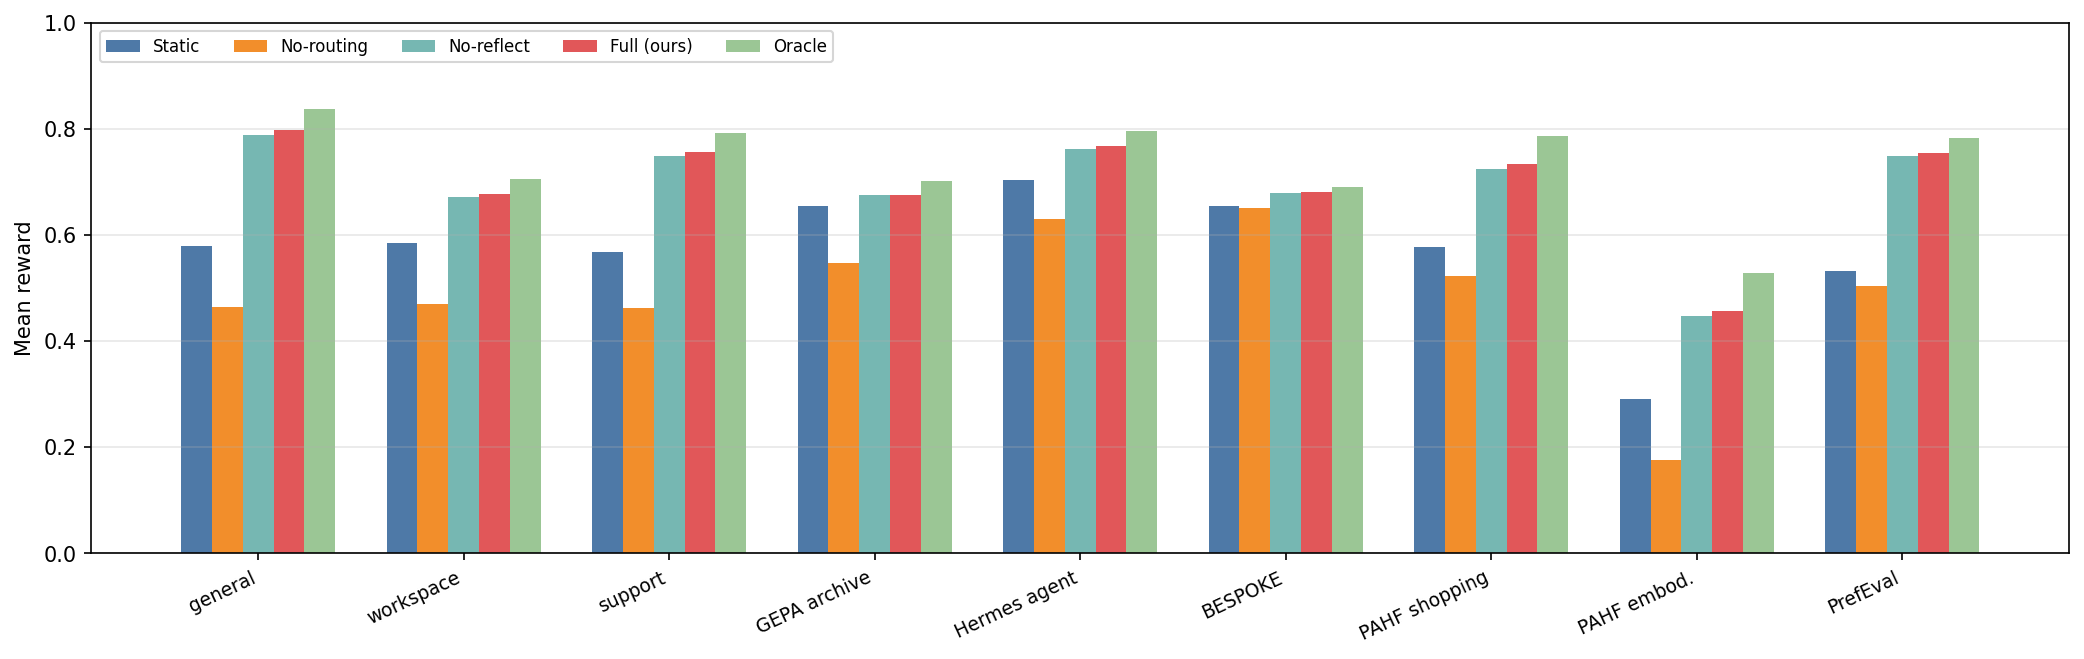
\includegraphics[width=\columnwidth]{fig_ablation_9benchmarks.png}
\caption{Mean reward by ablation variant across all nine benchmarks. Removing routing collapses reward; reflection and personalization features provide smaller incremental gains.}
\label{fig:ablation}
\end{figure}

\paragraph{Per-round convergence.} Figure~\ref{fig:perround-matrix} shows per-round reward traces for each benchmark.

In all cases, PersonalEvo converges toward the oracle within ${\sim}50$ rounds, while the static baseline remains flat.

The exploration cost $\widehat L_t$ decays sublinearly, consistent with the $O(\sqrt{K_{\max} d T \log T})$ rate of Corollary~\ref{cor:plugin}.

\begin{figure}[h]
\centering
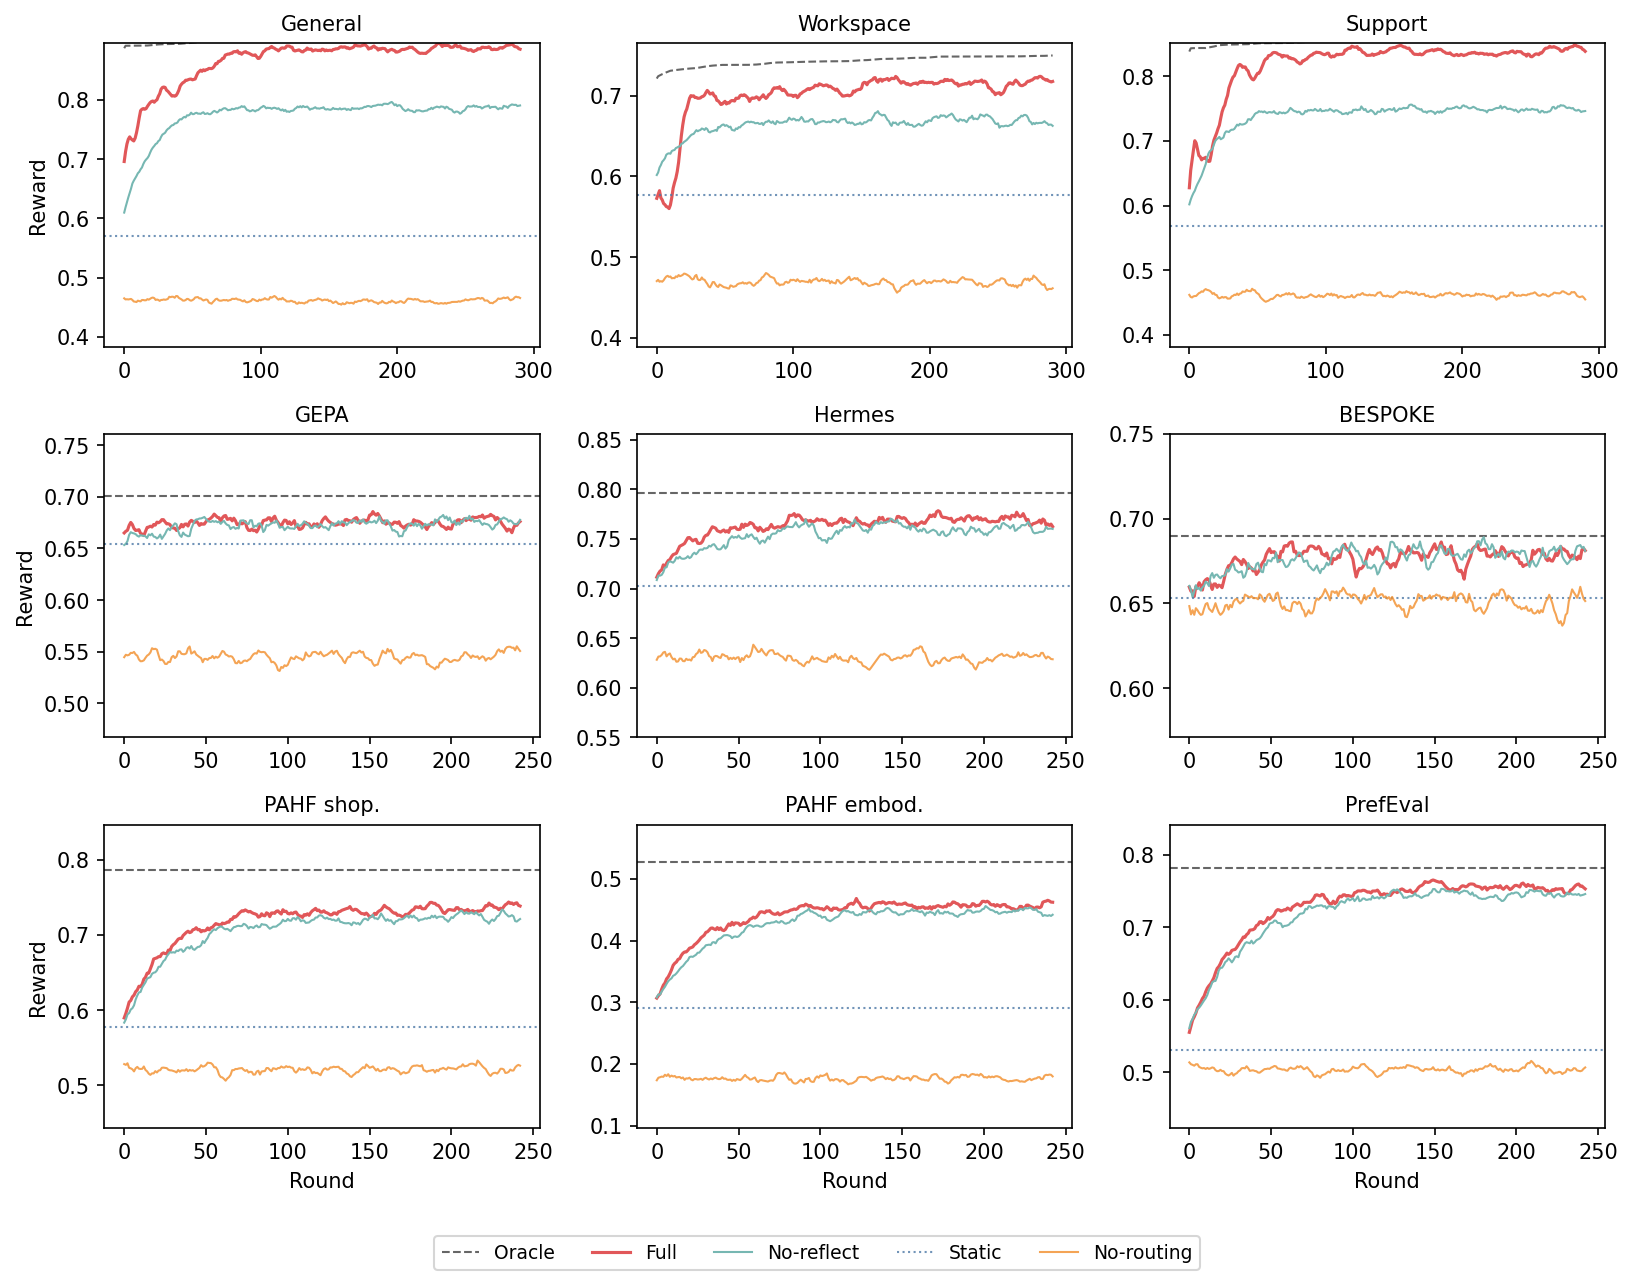
\includegraphics[width=\columnwidth]{fig_perround_3x3_matrix.png}
\caption{Per-round reward for all nine benchmarks (3$\times$3 grid). Five variants shown: \textbf{Full} (red; concat features, gated reflection, LinUCB), \textbf{No-reflect} (teal; frozen archive, $\bar G_T{=}0$), \textbf{No-routing} (orange; uniform-random selection, $\Delta_{\mathrm{route}}{\to}0$), \textbf{Static} (gray dotted; best single candidate for all users), \textbf{Oracle} (black dashed; per-user optimum). Top row: synthetic; middle and bottom: framework and real-data benchmarks.}
\label{fig:perround-matrix}\label{tab:variants}
\end{figure}

\subsection{Comparison against existing routing methods}

\label{sec:exp-baselines}

To position PersonalEvo against prior routing strategies, we compare five methods on all nine benchmarks (Table~\ref{tab:baselines}): (i)~\textbf{Static}: deploy the single best-on-average candidate; (ii)~\textbf{GEPA-Pareto}: maintain the Pareto-optimal subset of the archive and deploy uniformly from it \citep{agrawal2025geparp}; (iii)~\textbf{Thompson}: Bayesian Thompson sampling over candidates \citep{pahf2025}; (iv)~\textbf{RouteLLM-thresh}: route users to specialist or generalist candidates based on a variance threshold; (v)~\textbf{PersonalEvo}: our full method.

\begin{table}[h]
\centering
\small
\resizebox{\columnwidth}{!}{
\begin{tabular}{lccccccc}
\toprule
\textbf{Benchmark} & \textbf{Static} & \textbf{GEPA-Pareto} & \textbf{Thompson} & \textbf{RouteLLM} & \textbf{PersonalEvo} & \textbf{Oracle} \\
\midrule
General            & $0.579$ & $0.533$ & $0.510$ & $0.732$ & $\mathbf{0.797}$ & $0.836$ \\
Workspace          & $0.585$ & $0.539$ & $0.515$ & $0.650$ & $\mathbf{0.678}$ & $0.705$ \\
Support            & $0.568$ & $0.525$ & $0.504$ & $0.700$ & $\mathbf{0.757}$ & $0.791$ \\
GEPA archive       & $0.671$ & $0.616$ & $0.569$ & $0.675$ & $\mathbf{0.681}$ & $0.701$ \\
Hermes agent       & $0.729$ & $0.644$ & $0.659$ & $0.750$ & $\mathbf{0.771}$ & $0.796$ \\
BESPOKE            & $0.681$ & $0.660$ & $0.654$ & $0.678$ & $\mathbf{0.682}$ & $0.690$ \\
PAHF shopping      & $0.625$ & $0.532$ & $0.560$ & $0.691$ & $\mathbf{0.754}$ & $0.812$ \\
PAHF embodied      & $0.290$ & $0.244$ & $0.222$ & $0.407$ & $\mathbf{0.457}$ & $0.528$ \\
PrefEval           & $0.531$ & $0.520$ & $0.514$ & $0.687$ & $\mathbf{0.754}$ & $0.782$ \\
\bottomrule
\end{tabular}
}
\caption{Comparison against existing routing methods on all nine benchmarks. Mean reward over 5 seeds. PersonalEvo (bold) achieves the highest reward among non-oracle methods in every row. GEPA-Pareto underperforms static because archive diversity without per-user routing is counterproductive. Thompson sampling explores too broadly. RouteLLM-threshold is the closest competitor but uses a fixed rule rather than learning per-user preferences.}
\label{tab:baselines}
\end{table}

The results reveal why the decomposition matters for method design: GEPA-Pareto maintains a diverse archive ($\bar G_T$ is high) but has no routing mechanism to exploit $\Delta_{\mathrm{route}}$, so diversity is wasted.

Thompson sampling routes but explores every arm equally regardless of user context, paying excessive $\bar L_T$.

RouteLLM routes by context but uses a fixed threshold rather than learning individual preferences.

PersonalEvo combines per-user routing (exploiting $\Delta_{\mathrm{route}}$) with gated evolution (controlled $\bar G_T$) and low exploration cost (small $\bar L_T$), which is exactly the configuration the decomposition predicts will win.

\subsection{Hyper-Ridge diagnostics and the remaining evaluation gap}
\label{sec:exp-hyper-ridge-plan}

The decomposition estimates in Table~\ref{tab:main}, ablations in Figure~\ref{fig:ablation}, per-round traces in Figure~\ref{fig:perround-matrix}, and baseline comparison in Table~\ref{tab:baselines} all evaluate the \emph{base} PersonalEvo router. We additionally ran a five-seed diagnostic suite for Hyper-Ridge PersonalEvo. We keep it separate from the headline comparison because it covers seven rather than nine adapters and does not yet measure the full decomposition with exploration cost as the primary endpoint.

\paragraph{Known-geometry mechanism.}
We first construct a well-specified linear bandit in which $K=30$ candidate parameters are drawn from a planted rank-three covariance, contexts are dense random unit vectors, and the horizon is $T=400$. Table~\ref{tab:hyper-diagnostic} compares isotropic ridge, Hyper-Ridge given the true covariance, and Hyper-Ridge with the covariance periodically re-estimated from the candidate models, all with the same ridge weight $\lambda=0.5$. The oracle geometry cuts cumulative exploration cost by $46$--$59\%$ as the ambient dimension grows, consistent with the effective-dimension mechanism. The online estimate instead raises cost by $7$--$19\%$. The experiment therefore validates the benefit of the right geometry, while locating the current failure in estimating it.

\begin{table}[H]
\centering
\small
\begin{tabular}{rrrrr}
\toprule
$d$ & Isotropic & Known $\Omega$ & Estimated $\Omega$ & Known-$\Omega$ reduction \\
\midrule
20  & 314.1 & 170.2 & 375.0 & $45.8\%$ \\
50  & 447.6 & 213.1 & 504.9 & $52.4\%$ \\
100 & 455.4 & 188.1 & 487.5 & $58.7\%$ \\
\bottomrule
\end{tabular}
\caption{Mean cumulative exploration cost over five seeds on planted rank-three problems ($K=30$, $T=400$, $\lambda=0.5$ for all three routers). Lower is better. The true geometry realizes the predicted benefit; periodic online estimation does not.}
\label{tab:hyper-diagnostic}
\end{table}

\paragraph{Adapter diagnostic.}
With tuning seeds disjoint from the five reporting seeds, the periodic estimator improves mean reward over the isotropic router on six of seven adapters, with changes ranging from $+0.002$ on BESPOKE to $+0.048$ on Hermes, and loses $0.010$ on GEPA. These numbers are not evidence of cross-candidate geometry transfer. The adapter harness represents candidate $a$ by the one-hot vector $e_a$. Starting from $\widehat{\Omega}_1=I$, each candidate estimate then has support only on its own coordinate, so the covariance update remains diagonal. Accordingly, the full-covariance and diagonal-ridge variants match exactly on every adapter and seed. This ablation exposes a representation mismatch that a larger seed count cannot repair.

\paragraph{Remaining protocol.}
The complete comparison must run base, known-covariance, calibration-split estimated-covariance, periodically estimated-covariance, and diagonal-ridge routers on the same nine benchmarks, using a feature map with shared behavioral directions. It must report all four terms of \eqref{eq:method-thesis}, with $\widehat L_T$ as the primary endpoint, as well as the fitted regret exponent, covariance error, and $d_{\mathrm{eff}}(\widehat\Omega)$. Until that comparison is complete, we do not claim an empirical advantage for the fully adaptive Hyper-Ridge router.

\paragraph{Implementation status.}
The repository implements both the base router and the periodic Hyper-Ridge estimator, together with an identity-reduction test showing that frozen $\widehat{\Omega}=I$ reproduces the base router selection for selection. The diagnostic results are stored in \texttt{results/hyper\_ridge/suite.json}; the missing component is the feature-aware, nine-benchmark evaluation above, not the router implementation itself.

\section{Conclusion}

\label{sec:conclusion}

This paper revised the PersonalEvo framework around a single idea: a self-evolving agent should meta-learn the geometry of its own archive. The base framework answers \emph{whether} personalized routing pays off through the exact four-term decomposition
\begin{equation}
\label{eq:conc-decomp}
\frac{1}{T}\sum_{t=1}^{T}\E\bigl[\mu(U,a_t(U))\bigr]
\;=\;
V_{\mathrm{static}}(A_1)
+ \Delta_{\mathrm{route}}(A_1)
+ \bar G_T
- \bar L_T,
\end{equation}
and the associated dominance condition
\begin{equation}
\label{eq:conc-dom}
\Delta_{\mathrm{route}}(A_1) + \bar G_T \;>\; \bar L_T,
\end{equation}
both of which are inherited unchanged from the base paper (Theorem~\ref{thm:decomp}, Corollary~\ref{cor:dominance}). The revision leaves the first three terms untouched and attacks the only negative term. The base router treats archive candidates as independent LinUCB arms with an identity-regularized ridge solve, paying an exploration cost governed by the ambient feature dimension,
\begin{equation}
\label{eq:conc-base-rate}
\sum_{t=1}^{T}\E[L_t(U)]
\;=\;
O\!\left(\sqrt{K_{\max}\, d\, T \log T}\right).
\end{equation}
Hyper-Ridge PersonalEvo instead models candidate parameters as random effects sharing a hyper-covariance,
\begin{equation}
\label{eq:conc-random-effects}
\theta_a \sim (0,\Omega), \qquad \Omega \in \mathbb{R}^{d\times d},
\end{equation}
estimates $\widehat\Omega_t$ from pooled archive data, and uses it as the generalized-ridge geometry inside the UCB score. The resulting exploration-cost target replaces $d$ by the effective dimension of the archive,
\begin{equation}
\label{eq:conc-deff}
d_{\mathrm{eff}}(\Omega)
\;=\;
\operatorname{tr}\!\left[
X^\top X \left(X^\top X + \lambda \Omega^{-1}\right)^{-1}
\right],
\end{equation}
yielding, under the low-dimensional shared-structure regime and modulo the covariance-estimation error term,
\begin{equation}
\label{eq:conc-hyper-rate}
\sum_{t=1}^{T}\E[L_t(U)]
\;\lesssim\;
\sqrt{K_{\max}\, d_{\mathrm{eff}}(\Omega)\, T \log T}
\;+\;
\mathrm{Err}_T(\widehat\Omega, \Omega).
\end{equation}
When $d_{\mathrm{eff}}(\Omega) \ll d$, the dominance condition \eqref{eq:conc-dom} is satisfied in strictly more regimes, so archive evolution can contribute twice: newly evolved candidates raise $\bar G_T$, and sufficiently informative archive data can sharpen $\widehat\Omega_t$ and lower $\bar L_T$. The generalized-ridge estimator, effective-dimension bound, and diagnostic suite all test this thesis, while the estimated-covariance results show that the second benefit is not automatic.

Two provenance facts bound what this paper claims. First, the nine-benchmark decomposition estimates, ablation hierarchy, per-round convergence traces, and baseline comparison in Section~\ref{sec:experiments} belong to the \emph{base} LinUCB router. They validate the inherited decomposition \eqref{eq:conc-decomp} and dominance condition \eqref{eq:conc-dom}, with margins
\begin{equation}
\label{eq:conc-margins}
\Delta_{\mathrm{route}}(A_1) + \bar G_T - \bar L_T \;\in\; [+0.027,\, +0.295]
\end{equation}
across all nine benchmarks, and they confirm that the routing gain exceeds the evolution gain in every row. The separate Hyper-Ridge suite is diagnostic: known geometry helps on planted low-rank problems, but periodic estimation does not recover that benefit, and one-hot adapters collapse the full covariance to a diagonal one. Second, the effective-dimension guarantee \eqref{eq:conc-hyper-rate} is a theorem for the oracle-covariance router. Appendix~\ref{app:err-control-proof} controls an estimated covariance for a calibration-split procedure under explicit diversity conditions, but this result does not cover the periodically updated estimator in Algorithm~\ref{alg:hyper-ridge}. Controlling that fully adaptive estimator remains the primary theoretical open problem.

The corresponding empirical open problem is the complete comparison specified in Section~\ref{sec:exp-hyper-ridge-plan}: base LinUCB versus known-covariance, calibration-split, periodically estimated, and diagonal-ridge routers on the same nine benchmarks, with the exploration cost $\widehat L_T$ as the primary endpoint. The feature map must admit shared directions; otherwise the full model is diagonal by construction. The comparison should also report covariance error, the fitted regret exponent, and a per-benchmark estimate of $d_{\mathrm{eff}}(\widehat\Omega)$ to locate both sides of the boundary: regimes where
\begin{equation}
\label{eq:conc-regime}
d_{\mathrm{eff}}(\Omega) \ll d
\end{equation}
and the hyper-ridge router should dominate, and near-isotropic regimes where $d_{\mathrm{eff}}(\Omega)\approx d$ and covariance estimation can only add cost. The current implementation supplies the periodic estimator and common harness; a calibration-split implementation and a shared feature representation remain to be added.

Beyond the two named gaps, the limitations of the base framework carry over. The reflective proposer in the simulated environments is oracle-assisted, so the measured evolution gain $\bar G_T$ is an upper bound on what a realistic LLM-driven proposer would deliver, and each user maintains a private archive, so discoveries are not shared across users. The hyper-ridge extension makes the second limitation more interesting rather than less: a shared evolving archive would pool more data into $\widehat\Omega_t$, potentially shrinking $\mathrm{Err}_T(\widehat\Omega,\Omega)$ at a population rate, but it changes the predictability analysis underlying Lemma~\ref{lem:predictable} and is deferred. More broadly, the decomposition \eqref{eq:conc-decomp} applies to any system that maintains a candidate library and must decide what to serve to whom (model routing, prompt selection, tool-use policies), and the message of this revision applies with it: such libraries are structured objects, not unordered bags of candidates, and estimating their latent geometry is a direct, quantifiable lever on the one term in the accounting that works against personalization.

\appendix

\section{Appendix Proofs: Preliminaries and the Exact Decomposition}

\label{app:proofs}

This appendix block fixes the probability model used by all proofs and proves the first main theorem: the exact four-term decomposition.

The proof is an accounting identity; it does not use a contextual-bandit regret theorem and does not assume that reflection is realistic.

\subsection{Probability space and online objects}

All random variables below are defined on one probability space:

\begin{equation}
\label{eq:app-probability-space}
(\Omega,\mathcal{F},\mathbb{P}).
\end{equation}

All expectations are taken over both the population draw and the online trajectory:

\begin{equation}
\label{eq:app-expectation}
\mathbb{E}[Z]
=
\int_{\Omega} Z(\omega)\,d\mathbb{P}(\omega).
\end{equation}

The evaluation user is drawn from a population distribution:

\begin{equation}
\label{eq:app-user-draw}
U \sim \Pi.
\end{equation}

The user takes values in a measurable user space:

\begin{equation}
\label{eq:app-user-space}
U:\Omega \to \mathcal{U}.
\end{equation}

The candidate universe is denoted by

\begin{equation}
\label{eq:app-candidate-universe}
\mathcal{A}.
\end{equation}

The common initial archive is

\begin{equation}
\label{eq:app-initial-archive}
A_1 \subseteq \mathcal{A}.
\end{equation}

The current archive before round \(t\) is

\begin{equation}
\label{eq:app-current-archive}
A_t(U) \subseteq \mathcal{A}.
\end{equation}

The router's deployed candidate is

\begin{equation}
\label{eq:app-action}
a_t(U) \in A_t(U).
\end{equation}

The mean reward function is

\begin{equation}
\label{eq:app-mean-reward}
\mu:\mathcal{U}\times\mathcal{A}\to[0,1].
\end{equation}

The observed reward is

\begin{equation}
\label{eq:app-observed-reward}
r_t
=
\mu(U,a_t(U))+\xi_t.
\end{equation}

For later plug-in bounds, the online filtration is

\begin{equation}
\label{eq:app-filtration}
\mathcal{F}_0 \subseteq \mathcal{F}_1 \subseteq \cdots \subseteq \mathcal{F}_T.
\end{equation}

Feature vectors used by the disjoint LinUCB implementation are denoted by

\begin{equation}
\label{eq:app-feature-vector}
x_t(a)\in\mathbb{R}^{d}.
\end{equation}

Only the boundedness and archive assumptions are used in the four-term decomposition proof; the noise and feature assumptions are recorded here so later proof chunks can refer back to the same notation.

\begin{assumption}[A1: bounded mean reward]
\label{ass:app-bounded}
For every user and candidate, the mean reward satisfies
\begin{equation}
\label{eq:app-ass-bounded}
0 \,\le\, \mu(u,a) \,\le\, 1.
\end{equation}
\end{assumption}

\begin{assumption}[A2: finite common initial archive]
\label{ass:app-finite-initial}
The initial archive is nonempty and finite:
\begin{equation}
\label{eq:app-ass-initial-finite}
1 \,\le\, |A_1| < \infty.
\end{equation}
\end{assumption}

\begin{assumption}[A3: finite append-only online archives]
\label{ass:app-append-only}
For every round, the current archive is nonempty and finite almost surely:
\begin{equation}
\label{eq:app-ass-current-finite}
1 \,\le\, |A_t(U)| < \infty.
\end{equation}
The archive process is append-only:
\begin{equation}
\label{eq:app-ass-append-only}
A_t(U)\subseteq A_{t+1}(U).
\end{equation}
\end{assumption}

\begin{assumption}[A4: predictable archive]
\label{ass:app-predictable}
Before choosing the round-\(t\) candidate, the archive is measurable with respect to the past:
\begin{equation}
\label{eq:app-ass-predictable}
\sigma(A_t(U)) \subseteq \mathcal{F}_{t-1}.
\end{equation}
\end{assumption}

\begin{assumption}[A5: centered conditionally sub-Gaussian noise]
\label{ass:app-noise}
The reward noise is conditionally centered:
\begin{equation}
\label{eq:app-ass-noise-mean}
\mathbb{E}[\xi_t\mid \mathcal{F}_{t-1}] = 0.
\end{equation}
For every real scalar \(\lambda\), the conditional moment generating function obeys
\begin{equation}
\label{eq:app-ass-noise-subg}
\mathbb{E}\!\left[\exp(\lambda \xi_t)\mid \mathcal{F}_{t-1}\right]
\,\le\,
\exp\!\left(\frac{\lambda^2\sigma^2}{2}\right).
\end{equation}
\end{assumption}

\begin{assumption}[A6: bounded features]
\label{ass:app-features}
For every available candidate, the feature norm is bounded:
\begin{equation}
\label{eq:app-ass-feature-bound}
\|x_t(a)\|_2 \,\le\, L.
\end{equation}
\end{assumption}

\subsection{Values and accounting terms}

For any deterministic finite archive, the best static value is

\begin{equation}
\label{eq:app-vstatic}
V_{\mathrm{static}}(A)
=
\max_{a\in A}\mathbb{E}[\mu(U,a)].
\end{equation}

For the same archive, the perfect routed value is

\begin{equation}
\label{eq:app-vroute}
V_{\mathrm{route}}(A)
=
\mathbb{E}\!\left[\max_{a\in A}\mu(U,a)\right].
\end{equation}

The fixed-archive heterogeneity gain is

\begin{equation}
\label{eq:app-delta-het}
\Delta_{\mathrm{route}}(A)
=
V_{\mathrm{route}}(A)-V_{\mathrm{static}}(A).
\end{equation}

The current-archive oracle value for the realized user is

\begin{equation}
\label{eq:app-mt}
m_t(U)
=
\max_{a\in A_t(U)} \mu(U,a).
\end{equation}

The discovery gain at round \(t\) is

\begin{equation}
\label{eq:app-gt}
G_t(U)
=
m_t(U)-m_1(U).
\end{equation}

The exploration cost at round \(t\) is

\begin{equation}
\label{eq:app-lt}
L_t(U)
=
m_t(U)-\mu(U,a_t(U)).
\end{equation}

The horizon-averaged discovery gain is

\begin{equation}
\label{eq:app-barg}
\bar G_T
=
\frac{1}{T}\sum_{t=1}^{T}\mathbb{E}[G_t(U)].
\end{equation}

The horizon-averaged exploration cost is

\begin{equation}
\label{eq:app-barl}
\bar L_T
=
\frac{1}{T}\sum_{t=1}^{T}\mathbb{E}[L_t(U)].
\end{equation}

\begin{proposition}[Integrability and signs of the accounting terms]
\label{prop:1}
Under Assumptions~\ref{ass:app-bounded}--\ref{ass:app-append-only}, the current-archive optimum satisfies
\begin{equation}
\label{eq:app-prop-m-bound}
0 \,\le\, m_t(U) \,\le\, 1.
\end{equation}
The exploration cost satisfies
\begin{equation}
\label{eq:app-prop-l-bound}
0 \,\le\, L_t(U) \,\le\, 1.
\end{equation}
The discovery gain satisfies
\begin{equation}
\label{eq:app-prop-g-bound}
0 \,\le\, G_t(U) \,\le\, 1.
\end{equation}
Consequently all three terms are integrable:
\begin{equation}
\label{eq:app-prop-integrable}
\mathbb{E}[|m_t(U)|]+\mathbb{E}[|G_t(U)|]+\mathbb{E}[|L_t(U)|] \,\le\, 3.
\end{equation}
\end{proposition}

\begin{proof}
Assumption~\ref{ass:app-bounded} gives the pointwise reward bound:
\begin{align}
\label{eq:app-prop-proof-reward-bound}
0
\,\le\,
\mu(U,a)
\,\le\,
1
\qquad
\text{for every } a\in\mathcal{A}.
\end{align}
Taking a maximum over a finite nonempty archive preserves the same interval:
\begin{align}
\label{eq:app-prop-proof-m-bound}
0
\,\le\,
\max_{a\in A_t(U)}\mu(U,a)
\,\le\,
1.
\end{align}
Using \eqref{eq:app-mt}, this is
\begin{align}
\label{eq:app-prop-proof-m}
0
\,\le\,
m_t(U)
\,\le\,
1.
\end{align}
Since the deployed candidate belongs to the current archive, we have
\begin{align}
\label{eq:app-prop-proof-action-in-archive}
\mu(U,a_t(U))
\,\le\,
\max_{a\in A_t(U)}\mu(U,a).
\end{align}
Therefore
\begin{align}
\label{eq:app-prop-proof-l-lower}
L_t(U)
&\,=\,
m_t(U)-\mu(U,a_t(U))
\\
&\,\ge\,
0.
\end{align}
The upper bound follows from the reward range:
\begin{align}
\label{eq:app-prop-proof-l-upper}
L_t(U)
&\,=\,
m_t(U)-\mu(U,a_t(U))
\\
&\,\le\,
1-0
\\
&\,=\,
1.
\end{align}
The append-only condition implies that the initial archive remains available:
\begin{align}
\label{eq:app-prop-proof-monotone}
A_1
\subseteq
A_t(U).
\end{align}
Thus the current optimum dominates the initial optimum:
\begin{align}
\label{eq:app-prop-proof-g-lower}
m_t(U)
&\,=\,
\max_{a\in A_t(U)}\mu(U,a)
\\
&\,\ge\,
\max_{a\in A_1}\mu(U,a)
\\
&\,=\,
m_1(U).
\end{align}
Hence
\begin{align}
\label{eq:app-prop-proof-g-nonnegative}
G_t(U)
=
m_t(U)-m_1(U)
\,\ge\,
0.
\end{align}
The upper bound is again inherited from the reward range:
\begin{align}
\label{eq:app-prop-proof-g-upper}
G_t(U)
&\,=\,
m_t(U)-m_1(U)
\\
&\,\le\,
1-0
\\
&\,=\,
1.
\end{align}
Combining the three interval bounds gives
\begin{align}
\label{eq:app-prop-proof-integrable}
\mathbb{E}[|m_t(U)|]+\mathbb{E}[|G_t(U)|]+\mathbb{E}[|L_t(U)|]
&\,\le\,
1+1+1
\\
&\,=\,
3.
\end{align}
\end{proof}

\subsection{Supporting lemmas for the four-term decomposition}

\begin{lemma}[Static-versus-routed value]
\label{lem:1}
Let \(A\) be any deterministic finite nonempty archive:
\begin{equation}
\label{eq:app-lem1-archive}
1 \,\le\, |A| < \infty.
\end{equation}
Define its pointwise routed optimum by
\begin{equation}
\label{eq:app-lem1-h}
h_A(U)
=
\max_{a\in A}\mu(U,a).
\end{equation}
Define the static value by
\begin{equation}
\label{eq:app-lem1-static}
V_{\mathrm{static}}(A)
=
\max_{a\in A}\mathbb{E}[\mu(U,a)].
\end{equation}
Define the routed value by
\begin{equation}
\label{eq:app-lem1-route}
V_{\mathrm{route}}(A)
=
\mathbb{E}[h_A(U)].
\end{equation}
Define the heterogeneity gap by
\begin{equation}
\label{eq:app-lem1-gap}
\Delta_{\mathrm{route}}(A)
=
V_{\mathrm{route}}(A)-V_{\mathrm{static}}(A).
\end{equation}
Then
\begin{equation}
\label{eq:app-lem1-nonnegative}
\Delta_{\mathrm{route}}(A)\,\ge\, 0.
\end{equation}
Moreover, equality holds if and only if there exists a candidate \(a^\star\in A\) such that
\begin{equation}
\label{eq:app-lem1-equality-condition}
\mu(U,a^\star)
=
\max_{a\in A}\mu(U,a)
\quad
\text{almost surely}.
\end{equation}
In particular, the inequality is strict whenever every candidate fails to be pointwise optimal on a set of positive probability:
\begin{equation}
\label{eq:app-lem1-strict-condition}
\forall a\in A,
\qquad
\mathbb{P}\!\left(
\mu(U,a)
<
\max_{b\in A}\mu(U,b)
\right)
>
0.
\end{equation}
\end{lemma}

\begin{proof}
For every fixed candidate, the pointwise maximum dominates its reward:
\begin{align}
\label{eq:app-lem1-proof-pointwise}
h_A(U)
&\,=\,
\max_{b\in A}\mu(U,b)
\\
&\,\ge\,
\mu(U,a).
\end{align}
Taking expectations preserves the inequality:
\begin{align}
\label{eq:app-lem1-proof-expectation}
\mathbb{E}[h_A(U)]
&\,\ge\,
\mathbb{E}[\mu(U,a)].
\end{align}
Maximizing the right-hand side over the finite archive gives
\begin{align}
\label{eq:app-lem1-proof-max}
\mathbb{E}[h_A(U)]
&\,\ge\,
\max_{a\in A}\mathbb{E}[\mu(U,a)].
\end{align}
Substituting the definitions yields the weak inequality:
\begin{align}
\label{eq:app-lem1-proof-gap}
\Delta_{\mathrm{route}}(A)
&\,=\,
V_{\mathrm{route}}(A)-V_{\mathrm{static}}(A)
\\
&\,=\,
\mathbb{E}[h_A(U)]-\max_{a\in A}\mathbb{E}[\mu(U,a)]
\\
&\,\ge\,
0.
\end{align}
Because the archive is finite, the static maximizer set is nonempty:
\begin{align}
\label{eq:app-lem1-proof-argmax}
\operatorname*{arg\,max}_{a\in A}\mathbb{E}[\mu(U,a)]
\ne
\varnothing.
\end{align}
Choose one static maximizer:
\begin{align}
\label{eq:app-lem1-proof-astar}
a^\star
\in
\operatorname*{arg\,max}_{a\in A}\mathbb{E}[\mu(U,a)].
\end{align}
For this maximizer, the gap can be written as an expectation of a nonnegative random variable:
\begin{align}
\label{eq:app-lem1-proof-nonnegative-integrand}
\Delta_{\mathrm{route}}(A)
&\,=\,
\mathbb{E}[h_A(U)]-\mathbb{E}[\mu(U,a^\star)]
\\
&\,=\,
\mathbb{E}\!\left[h_A(U)-\mu(U,a^\star)\right].
\end{align}
The integrand is nonnegative:
\begin{align}
\label{eq:app-lem1-proof-integrand-geq}
h_A(U)-\mu(U,a^\star)
\,\ge\,
0.
\end{align}
A nonnegative random variable has zero expectation exactly when it is zero almost surely:
\begin{align}
\label{eq:app-lem1-proof-zero-iff}
\Delta_{\mathrm{route}}(A)=0
\quad
\Longleftrightarrow
\quad
h_A(U)-\mu(U,a^\star)=0
\ \text{almost surely}.
\end{align}
Using the definition of \(h_A\), this is precisely
\begin{align}
\label{eq:app-lem1-proof-equality-condition}
\mu(U,a^\star)
=
\max_{a\in A}\mu(U,a)
\quad
\text{almost surely}.
\end{align}
Conversely, if some candidate is pointwise optimal almost surely, then
\begin{align}
\label{eq:app-lem1-proof-converse}
V_{\mathrm{route}}(A)
&\,=\,
\mathbb{E}\!\left[\max_{a\in A}\mu(U,a)\right]
\\
&\,=\,
\mathbb{E}[\mu(U,a^\star)]
\\
&\,\le\,
\max_{a\in A}\mathbb{E}[\mu(U,a)]
\\
&\,=\,
V_{\mathrm{static}}(A).
\end{align}
Together with \eqref{eq:app-lem1-nonnegative}, this forces equality:
\begin{align}
\label{eq:app-lem1-proof-converse-equality}
V_{\mathrm{route}}(A)
=
V_{\mathrm{static}}(A).
\end{align}
Finally, if \eqref{eq:app-lem1-strict-condition} holds, then every possible static maximizer has strictly positive probability of being suboptimal:
\begin{align}
\label{eq:app-lem1-proof-strict}
\mathbb{P}\!\left(h_A(U)-\mu(U,a^\star)>0\right)
>
0.
\end{align}
Since the integrand is nonnegative and positive with positive probability, its expectation is positive:
\begin{align}
\label{eq:app-lem1-proof-positive}
\Delta_{\mathrm{route}}(A)
=
\mathbb{E}\!\left[h_A(U)-\mu(U,a^\star)\right]
>
0.
\end{align}
\end{proof}

\begin{lemma}[Pointwise routed-value accounting]
\label{lem:2}
For every round \(t\), define the current optimum by
\begin{equation}
\label{eq:app-lem2-mt}
m_t(U)
=
\max_{a\in A_t(U)}\mu(U,a).
\end{equation}
Define the discovery term by
\begin{equation}
\label{eq:app-lem2-gt}
G_t(U)
=
m_t(U)-m_1(U).
\end{equation}
Define the exploration-cost term by
\begin{equation}
\label{eq:app-lem2-lt}
L_t(U)
=
m_t(U)-\mu(U,a_t(U)).
\end{equation}
Then the deployed mean reward satisfies the pointwise identity
\begin{equation}
\label{eq:app-lem2-identity}
\mu(U,a_t(U))
=
m_1(U)+G_t(U)-L_t(U).
\end{equation}
\end{lemma}

\begin{proof}
Start from the definition of the exploration cost:
\begin{align}
\label{eq:app-lem2-proof-start}
L_t(U)
&\,=\,
m_t(U)-\mu(U,a_t(U)).
\end{align}
Rearrange the equality:
\begin{align}
\label{eq:app-lem2-proof-rearrange}
\mu(U,a_t(U))
&\,=\,
m_t(U)-L_t(U).
\end{align}
Use the definition of discovery gain:
\begin{align}
\label{eq:app-lem2-proof-discovery}
m_t(U)
&\,=\,
m_1(U)+G_t(U).
\end{align}
Substitute \eqref{eq:app-lem2-proof-discovery} into \eqref{eq:app-lem2-proof-rearrange}:
\begin{align}
\label{eq:app-lem2-proof-final}
\mu(U,a_t(U))
&\,=\,
m_1(U)+G_t(U)-L_t(U).
\end{align}
\end{proof}

\subsection{First main theorem: four-term decomposition}

\begin{theorem}[Exact decomposition over the common initial archive]
\label{thm:main}
This theorem restates the four-term decomposition used as Theorem~\ref{thm:decomp} in Section~\ref{sec:theory}.  The user is drawn as
\begin{equation}
\label{eq:app-thm-user}
U\sim \Pi.
\end{equation}
The initial archive is finite and nonempty:
\begin{equation}
\label{eq:app-thm-initial}
1\,\le\, |A_1|<\infty.
\end{equation}
At round \(t\), the deployed candidate belongs to the current archive:
\begin{equation}
\label{eq:app-thm-action}
a_t(U)\in A_t(U).
\end{equation}
The current archive optimum is
\begin{equation}
\label{eq:app-thm-mt}
m_t(U)
=
\max_{a\in A_t(U)}\mu(U,a).
\end{equation}
The discovery term is
\begin{equation}
\label{eq:app-thm-gt}
G_t(U)
=
m_t(U)-m_1(U).
\end{equation}
The exploration-cost term is
\begin{equation}
\label{eq:app-thm-lt}
L_t(U)
=
m_t(U)-\mu(U,a_t(U)).
\end{equation}
The static initial-archive value is
\begin{equation}
\label{eq:app-thm-vstatic}
V_{\mathrm{static}}(A_1)
=
\max_{a\in A_1}\mathbb{E}[\mu(U,a)].
\end{equation}
The routed initial-archive value is
\begin{equation}
\label{eq:app-thm-vroute}
V_{\mathrm{route}}(A_1)
=
\mathbb{E}\!\left[\max_{a\in A_1}\mu(U,a)\right].
\end{equation}
The initial-archive heterogeneity gain is
\begin{equation}
\label{eq:app-thm-delta}
\Delta_{\mathrm{route}}(A_1)
=
V_{\mathrm{route}}(A_1)-V_{\mathrm{static}}(A_1).
\end{equation}
Then each round satisfies
\begin{equation}
\label{eq:app-thm-per-round}
\mathbb{E}[\mu(U,a_t(U))]
=
V_{\mathrm{static}}(A_1)
+
\Delta_{\mathrm{route}}(A_1)
+
\mathbb{E}[G_t(U)]
-
\mathbb{E}[L_t(U)].
\end{equation}
Define the horizon-averaged routed value by
\begin{equation}
\label{eq:app-thm-rt}
R_T
=
\frac{1}{T}\sum_{t=1}^{T}\mathbb{E}[\mu(U,a_t(U))].
\end{equation}
Define the horizon-averaged discovery gain by
\begin{equation}
\label{eq:app-thm-barg}
\bar G_T
=
\frac{1}{T}\sum_{t=1}^{T}\mathbb{E}[G_t(U)].
\end{equation}
Define the horizon-averaged exploration cost by
\begin{equation}
\label{eq:app-thm-barl}
\bar L_T
=
\frac{1}{T}\sum_{t=1}^{T}\mathbb{E}[L_t(U)].
\end{equation}
Then the horizon-averaged decomposition is
\begin{equation}
\label{eq:app-decomp-bound}
R_T
=
V_{\mathrm{static}}(A_1)
+
\Delta_{\mathrm{route}}(A_1)
+
\bar G_T
-
\bar L_T.
\end{equation}
\end{theorem}

\begin{proof}
By Proposition~\ref{prop:1}, all quantities in the following expectations are integrable:
\begin{align}
\label{eq:app-thm-proof-integrability}
\mathbb{E}[|m_t(U)|]
+
\mathbb{E}[|G_t(U)|]
+
\mathbb{E}[|L_t(U)|]
&<
\infty.
\end{align}
Apply the pointwise accounting identity from Lemma~\ref{lem:2}:
\begin{align}
\label{eq:app-thm-proof-pointwise}
\mu(U,a_t(U))
&\,=\,
m_1(U)+G_t(U)-L_t(U).
\end{align}
Taking expectations gives
\begin{align}
\label{eq:app-thm-proof-expect}
\mathbb{E}[\mu(U,a_t(U))]
&\,=\,
\mathbb{E}[m_1(U)]
+
\mathbb{E}[G_t(U)]
-
\mathbb{E}[L_t(U)].
\end{align}
The first-archive optimum expands as
\begin{align}
\label{eq:app-thm-proof-m1}
\mathbb{E}[m_1(U)]
&\,=\,
\mathbb{E}\!\left[\max_{a\in A_1}\mu(U,a)\right]
\\
&\,=\,
V_{\mathrm{route}}(A_1).
\end{align}
By the definition of the heterogeneity gap,
\begin{align}
\label{eq:app-thm-proof-route-static}
V_{\mathrm{route}}(A_1)
&\,=\,
V_{\mathrm{static}}(A_1)
+
\Delta_{\mathrm{route}}(A_1).
\end{align}
Substituting \eqref{eq:app-thm-proof-route-static} into \eqref{eq:app-thm-proof-expect} yields the per-round identity:
\begin{align}
\label{eq:app-thm-proof-per-round}
\mathbb{E}[\mu(U,a_t(U))]
&\,=\,
V_{\mathrm{static}}(A_1)
+
\Delta_{\mathrm{route}}(A_1)
+
\mathbb{E}[G_t(U)]
-
\mathbb{E}[L_t(U)].
\end{align}
Average the previous display over the horizon:
\begin{align}
\label{eq:app-thm-proof-average-start}
\frac{1}{T}\sum_{t=1}^{T}\mathbb{E}[\mu(U,a_t(U))]
&\,=\,
\frac{1}{T}\sum_{t=1}^{T}
\left(
V_{\mathrm{static}}(A_1)
+
\Delta_{\mathrm{route}}(A_1)
+
\mathbb{E}[G_t(U)]
-
\mathbb{E}[L_t(U)]
\right)
\\
&\,=\,
V_{\mathrm{static}}(A_1)
+
\Delta_{\mathrm{route}}(A_1)
+
\frac{1}{T}\sum_{t=1}^{T}\mathbb{E}[G_t(U)]
-
\frac{1}{T}\sum_{t=1}^{T}\mathbb{E}[L_t(U)].
\end{align}
Using the definitions of \(R_T\), \(\bar G_T\), and \(\bar L_T\), this becomes
\begin{align}
\label{eq:app-thm-proof-average-final}
R_T
&\,=\,
V_{\mathrm{static}}(A_1)
+
\Delta_{\mathrm{route}}(A_1)
+
\bar G_T
-
\bar L_T.
\end{align}
\end{proof}

The theorem is an identity in mean rewards.

When Assumption~\ref{ass:app-noise} holds, the same expectation also governs observed rewards:

\begin{align}
\label{eq:app-observed-mean-link}
\mathbb{E}[r_t]
&\,=\,
\mathbb{E}[\mu(U,a_t(U))+\xi_t]
\\
&\,=\,
\mathbb{E}[\mu(U,a_t(U))]
+
\mathbb{E}[\xi_t]
\\
&\,=\,
\mathbb{E}[\mu(U,a_t(U))].
\end{align}

As a numerical check of the identity, the corrected \texttt{general} row in Table~\ref{tab:main} uses

\begin{equation}
\label{eq:app-numeric-static}
V_{\mathrm{static}}(A_1)=0.570.
\end{equation}

The measured heterogeneity term is

\begin{equation}
\label{eq:app-numeric-het}
\Delta_{\mathrm{route}}(A_1)=0.280.
\end{equation}

The measured discovery term is

\begin{equation}
\label{eq:app-numeric-discovery}
\bar G_T=0.051.
\end{equation}

The measured exploration-cost term is

\begin{equation}
\label{eq:app-numeric-tax}
\bar L_T=0.036.
\end{equation}

The decomposition therefore predicts

\begin{align}
\label{eq:app-numeric-closure}
V_{\mathrm{static}}(A_1)
+
\Delta_{\mathrm{route}}(A_1)
+
\bar G_T
-
\bar L_T
&\,=\,
0.570+0.280+0.051-0.036
\\
&\,=\,
0.865,
\end{align}

which matches the reported routed value \(0.864\) up to rounding and Monte Carlo error.

\section{Appendix Proofs: Second Main Theorem and Intermediate Lemmas}

\label{app:proofs2}

This section proves the second main theorem, the conditional plug-in statement for the exploration cost.

The proof does not assert a new regret rate; it shows how any valid bound on the cumulative exploration cost plugs into the four-term decomposition of Theorem~\ref{thm:main}.

\begin{assumption}[External expected exploration-cost bound]
\label{ass:app-external-tax}
The horizon is
\begin{equation}
\label{eq:app-tax-horizon}
T\in \mathbb{N}.
\end{equation}
The current archive optimum is
\begin{equation}
\label{eq:app-tax-current-optimum}
m_t(U)
=
\max_{a\in A_t(U)}\mu(U,a).
\end{equation}
The exploration cost is
\begin{equation}
\label{eq:app-tax-definition}
L_t(U)
=
m_t(U)-\mu(U,a_t(U)).
\end{equation}
There exists a deterministic sequence satisfying
\begin{equation}
\label{eq:app-external-tax-bound}
B_T\,\ge\, 0.
\end{equation}
The expected cumulative exploration cost is bounded as
\begin{equation}
\label{eq:app-external-tax-assumption}
\sum_{t=1}^{T}\mathbb{E}[L_t(U)]
\,\le\,
B_T.
\end{equation}
\end{assumption}

The next lemma records the conditioning fact that makes growing archives compatible with standard martingale arguments, provided children are appended only after the current reward is observed.

\begin{lemma}[Predictable archive conditioning]
\label{lem:3}
Define the pre-action sigma-field by
\begin{equation}
\label{eq:app-filtration-pre}
\mathcal{H}_{t-1}
=
\sigma\!\left(
U,\,
A_1,\,
\{a_s(U),r_s,A_{s+1}(U):1\,\le\, s<t\}
\right).
\end{equation}
Assume the archive is predictable:
\begin{equation}
\label{eq:app-predictable-archive}
A_t(U)\in \mathcal{H}_{t-1}.
\end{equation}
The feature vector for an available candidate is
\begin{equation}
\label{eq:app-feature-definition}
x_t(a)
=
\psi(U,a).
\end{equation}
Assume the feature vector is predictable:
\begin{equation}
\label{eq:app-feature-predictable}
x_t(a)\in \mathcal{H}_{t-1}
\quad
\text{for every }a\in A_t(U).
\end{equation}
Assume the selected candidate is predictable:
\begin{equation}
\label{eq:app-action-predictable}
a_t(U)\in \mathcal{H}_{t-1}.
\end{equation}
The observed reward noise satisfies
\begin{equation}
\label{eq:app-noise-zero-mean}
\mathbb{E}[\xi_t\mid \mathcal{H}_{t-1}]
=
0.
\end{equation}
It also satisfies the conditional sub-Gaussian bound
\begin{equation}
\label{eq:app-noise-subg}
\mathbb{E}\!\left[\exp(s\xi_t)\mid \mathcal{H}_{t-1}\right]
\,\le\,
\exp\!\left(\frac{s^2\sigma^2}{2}\right)
\quad
\text{for all }s\in\mathbb{R}.
\end{equation}
For any realized candidate \(a\), define the vector increment
\begin{equation}
\label{eq:app-mart-increment}
Z_{t,a}
=
\mathbf{1}\{a_t(U)=a\}\,x_t(a)\,\xi_t.
\end{equation}
Define the cumulative noise process
\begin{equation}
\label{eq:app-mart-process}
M_{n,a}
=
\sum_{t=1}^{n}Z_{t,a}.
\end{equation}
Then \(M_{n,a}\) is a vector-valued martingale with respect to the post-round filtration.
\end{lemma}

\begin{proof}
For the proof, write the selected action as
\begin{equation}
\label{eq:app-short-action}
a_t
=
a_t(U).
\end{equation}
Predictability gives
\begin{align}
\label{eq:app-mart-predictable-product}
\mathbf{1}\{a_t=a\}\,x_t(a)
&\in
\mathcal{H}_{t-1}.
\end{align}
Taking conditional expectation yields
\begin{align}
\label{eq:app-mart-zero}
\mathbb{E}[Z_{t,a}\mid \mathcal{H}_{t-1}]
&\,=\,
\mathbb{E}\!\left[
\mathbf{1}\{a_t=a\}\,x_t(a)\,\xi_t
\mid
\mathcal{H}_{t-1}
\right]
\\
&\,=\,
\mathbf{1}\{a_t=a\}\,x_t(a)\,
\mathbb{E}[\xi_t\mid \mathcal{H}_{t-1}]
\\
&\,=\,
0.
\end{align}
For any direction \(v\), the scalar increment satisfies
\begin{align}
\label{eq:app-mart-subg-direction}
\mathbb{E}\!\left[
\exp\!\left(s\,v^\top Z_{t,a}\right)
\mid
\mathcal{H}_{t-1}
\right]
&\,=\,
\mathbb{E}\!\left[
\exp\!\left(
s\,\mathbf{1}\{a_t=a\}\,v^\top x_t(a)\,\xi_t
\right)
\mid
\mathcal{H}_{t-1}
\right]
\\
&\,\le\,
\exp\!\left(
\frac{s^2\sigma^2}{2}
\mathbf{1}\{a_t=a\}
(v^\top x_t(a))^2
\right).
\end{align}
Thus the increments are conditionally mean-zero and conditionally sub-Gaussian in every predictable direction, so the partial sums form a vector-valued martingale.
\end{proof}

The following elementary conversion is useful because many router analyses produce high-probability regret bounds, whereas Theorem~\ref{thm:main} is stated in expectation.

\begin{lemma}[From high-probability tax to expected tax]
\label{lem:4}
Assume the mean reward is bounded:
\begin{equation}
\label{eq:app-bounded-mean-for-tax}
0\,\le\, \mu(U,a)\,\le\, 1.
\end{equation}
Define the cumulative exploration cost by
\begin{equation}
\label{eq:app-cumulative-tax}
S_T^{L}
=
\sum_{t=1}^{T}L_t(U).
\end{equation}
Suppose there is a number
\begin{equation}
\label{eq:app-highprob-tax}
\widetilde{B}_T\,\ge\, 0
\end{equation}
and a failure probability
\begin{equation}
\label{eq:app-highprob-delta}
\delta\in(0,1)
\end{equation}
such that
\begin{equation}
\label{eq:app-highprob-tax-event}
\mathbb{P}\!\left(S_T^{L}\,\le\, \widetilde{B}_T\right)
\,\ge\,
1-\delta.
\end{equation}
Then
\begin{equation}
\label{eq:app-highprob-to-expectation}
\sum_{t=1}^{T}\mathbb{E}[L_t(U)]
\,\le\,
\widetilde{B}_T+T\delta.
\end{equation}
\end{lemma}

\begin{proof}
Since \(a_t(U)\in A_t(U)\), the current optimum dominates the deployed mean:
\begin{align}
\label{eq:app-tax-nonnegative}
L_t(U)
&\,=\,
m_t(U)-\mu(U,a_t(U))
\\
&\,\ge\,
0.
\end{align}
The bounded-reward condition gives
\begin{align}
\label{eq:app-tax-upper}
L_t(U)
&\,=\,
m_t(U)-\mu(U,a_t(U))
\\
&\,\le\,
1.
\end{align}
Therefore
\begin{align}
\label{eq:app-cumulative-tax-range}
0
\,\le\,
S_T^{L}
\,\le\,
T.
\end{align}
Let the good event be
\begin{equation}
\label{eq:app-tax-good-event}
\mathcal{E}_T^{L}
=
\{S_T^{L}\,\le\, \widetilde{B}_T\}.
\end{equation}
Split the expectation over this event:
\begin{align}
\label{eq:app-tax-split}
\mathbb{E}[S_T^{L}]
&\,=\,
\mathbb{E}[S_T^{L}\mathbf{1}\{\mathcal{E}_T^{L}\}]
+
\mathbb{E}[S_T^{L}\mathbf{1}\{(\mathcal{E}_T^{L})^c\}]
\\
&\,\le\,
\widetilde{B}_T
+
T\,\mathbb{P}((\mathcal{E}_T^{L})^c)
\\
&\,\le\,
\widetilde{B}_T
+
T\delta.
\end{align}
Using the definition of \(S_T^{L}\), this is exactly
\begin{align}
\label{eq:app-tax-expectation-final}
\sum_{t=1}^{T}\mathbb{E}[L_t(U)]
&\,\le\,
\widetilde{B}_T+T\delta.
\end{align}
\end{proof}

We next give one sufficient route to Assumption~\ref{ass:app-external-tax}.

This proposition is not a new contribution of the paper; it is a standard disjoint-linear UCB certificate written only to clarify what must be true for the plug-in theorem to inherit a familiar rate.

\begin{proposition}[Disjoint-linear certificate for the external tax bound]
\label{prop:2}
The feature dimension is
\begin{equation}
\label{eq:app-lin-d}
d\in\mathbb{N}.
\end{equation}
The realized archive union is
\begin{equation}
\label{eq:app-realized-union}
\mathcal{A}_T(U)
=
\bigcup_{t=1}^{T}A_t(U).
\end{equation}
The realized archive size is bounded by
\begin{equation}
\label{eq:app-kmax}
|\mathcal{A}_T(U)|
\,\le\,
K_{\max}.
\end{equation}
The feature vector is
\begin{equation}
\label{eq:app-lin-feature}
x_t(a)
=
\psi(U,a)\in\mathbb{R}^{d}.
\end{equation}
The feature norm is bounded by
\begin{equation}
\label{eq:app-lin-feature-bound}
\|x_t(a)\|_2
\,\le\,
L_x.
\end{equation}
The regularization parameter satisfies
\begin{equation}
\label{eq:app-lin-lambda}
\lambda
\,\ge\,
L_x^2.
\end{equation}
Each realized arm has a parameter
\begin{equation}
\label{eq:app-lin-theta}
\theta_a^\star\in\mathbb{R}^{d}.
\end{equation}
The parameter norm is bounded by
\begin{equation}
\label{eq:app-lin-theta-bound}
\|\theta_a^\star\|_2
\,\le\,
S.
\end{equation}
The mean model is disjoint-linear:
\begin{equation}
\label{eq:app-lin-model}
\mu(U,a)
=
x_t(a)^\top\theta_a^\star.
\end{equation}
The observed reward is
\begin{equation}
\label{eq:app-lin-observed}
r_t
=
\mu(U,a_t(U))+\xi_t.
\end{equation}
The noise obeys \eqref{eq:app-noise-zero-mean} and \eqref{eq:app-noise-subg}.  The ridge matrix for arm \(a\) before round \(t\) is
\begin{equation}
\label{eq:app-ridge-matrix}
V_{t,a}
=
\lambda I_d
+
\sum_{s=1}^{t-1}
\mathbf{1}\{a_s(U)=a\}\,x_s(a)x_s(a)^\top.
\end{equation}
The ridge estimator is
\begin{equation}
\label{eq:app-ridge-estimator}
\widehat{\theta}_{t,a}
=
V_{t,a}^{-1}
\sum_{s=1}^{t-1}
\mathbf{1}\{a_s(U)=a\}\,x_s(a)r_s.
\end{equation}
For confidence level \(\delta\), define
\begin{equation}
\label{eq:app-beta}
\beta_T(\delta)
=
\sigma
\sqrt{
2\log\!\left(\frac{K_{\max}}{\delta}\right)
+
d\log\!\left(1+\frac{T L_x^2}{\lambda d}\right)
}
+
\sqrt{\lambda}\,S.
\end{equation}
The router selects by the disjoint UCB rule
\begin{equation}
\label{eq:app-ucb-rule}
a_t(U)
\in
\operatorname*{arg\,max}_{a\in A_t(U)}
\left\{
x_t(a)^\top\widehat{\theta}_{t,a}
+
\beta_T(\delta)
\sqrt{x_t(a)^\top V_{t,a}^{-1}x_t(a)}
\right\}.
\end{equation}
Then, with probability at least \(1-\delta\),
\begin{equation}
\label{eq:app-lin-highprob-tax}
\sum_{t=1}^{T}L_t(U)
\,\le\,
B_T^{\mathrm{lin}}(\delta),
\end{equation}
where
\begin{equation}
\label{eq:app-lin-bt}
B_T^{\mathrm{lin}}(\delta)
=
2\beta_T(\delta)
\sqrt{
2T K_{\max} d
\log\!\left(1+\frac{T L_x^2}{\lambda d}\right)
}.
\end{equation}
Consequently,
\begin{equation}
\label{eq:app-lin-expected-tax}
\sum_{t=1}^{T}\mathbb{E}[L_t(U)]
\,\le\,
B_T^{\mathrm{lin}}(\delta)+T\delta.
\end{equation}
\end{proposition}

\begin{proof}
For the proof, abbreviate the action by
\begin{equation}
\label{eq:app-prop-action-short}
a_t
=
a_t(U).
\end{equation}
For each realized arm \(a\), define the accumulated noise vector
\begin{equation}
\label{eq:app-prop-noise-vector}
M_{t,a}
=
\sum_{s=1}^{t-1}
\mathbf{1}\{a_s=a\}\,x_s(a)\xi_s.
\end{equation}
By Lemma~\ref{lem:3}, \(M_{t,a}\) is a vector-valued martingale over the predictable selection times of arm \(a\).  The self-normalized martingale inequality gives
\begin{align}
\label{eq:app-self-normalized}
\mathbb{P}\!\left(
\exists t\,\le\, T:
\|M_{t,a}\|_{V_{t,a}^{-1}}
>
\sigma
\sqrt{
2\log\!\left(\frac{K_{\max}}{\delta}\right)
+
\log\!\left(\frac{\det V_{t,a}}{\det(\lambda I_d)}\right)
}
\right)
&\,\le\,
\frac{\delta}{K_{\max}}.
\end{align}
The determinant ratio is bounded by the trace:
\begin{align}
\label{eq:app-det-bound}
\log\!\left(\frac{\det V_{t,a}}{\det(\lambda I_d)}\right)
&\,\le\,
d\log\!\left(
1+
\frac{1}{\lambda d}
\sum_{s=1}^{t-1}
\mathbf{1}\{a_s=a\}\|x_s(a)\|_2^2
\right)
\\
&\,\le\,
d\log\!\left(
1+\frac{T L_x^2}{\lambda d}
\right).
\end{align}
Union over at most \(K_{\max}\) realized arms gives the confidence event
\begin{equation}
\label{eq:app-confidence-event}
\mathcal{E}_T
=
\left\{
\forall t\,\le\, T,\,
\forall a\in A_t(U):
\left|
x_t(a)^\top(\widehat{\theta}_{t,a}-\theta_a^\star)
\right|
\,\le\,
\beta_T(\delta)
\sqrt{x_t(a)^\top V_{t,a}^{-1}x_t(a)}
\right\}.
\end{equation}
The previous displays imply
\begin{equation}
\label{eq:app-confidence-prob}
\mathbb{P}(\mathcal{E}_T)
\,\ge\,
1-\delta.
\end{equation}
On \(\mathcal{E}_T\), define the estimated mean by
\begin{equation}
\label{eq:app-estimated-mean}
\widehat{\mu}_t(a)
=
x_t(a)^\top\widehat{\theta}_{t,a}.
\end{equation}
Define the uncertainty width by
\begin{equation}
\label{eq:app-width}
z_t(a)
=
\sqrt{x_t(a)^\top V_{t,a}^{-1}x_t(a)}.
\end{equation}
Let the current archive oracle be
\begin{equation}
\label{eq:app-current-oracle-arm}
a_t^\star
\in
\operatorname*{arg\,max}_{a\in A_t(U)}\mu(U,a).
\end{equation}
Optimism and the UCB choice imply
\begin{align}
\label{eq:app-optimism-chain}
\mu(U,a_t^\star)
&\,\le\,
\widehat{\mu}_t(a_t^\star)
+
\beta_T(\delta)z_t(a_t^\star)
\\
&\,\le\,
\widehat{\mu}_t(a_t)
+
\beta_T(\delta)z_t(a_t)
\\
&\,\le\,
\mu(U,a_t)
+
2\beta_T(\delta)z_t(a_t).
\end{align}
Therefore the exploration cost obeys
\begin{align}
\label{eq:app-tax-width-bound}
L_t(U)
&\,=\,
\mu(U,a_t^\star)-\mu(U,a_t)
\\
&\,\le\,
2\beta_T(\delta)z_t(a_t).
\end{align}
The regularization condition gives
\begin{align}
\label{eq:app-width-at-most-one}
z_t(a_t)^2
&\,=\,
x_t(a_t)^\top V_{t,a_t}^{-1}x_t(a_t)
\\
&\,\le\,
\frac{\|x_t(a_t)\|_2^2}{\lambda}
\\
&\,\le\,
1.
\end{align}
Using Cauchy--Schwarz,
\begin{align}
\label{eq:app-cauchy-width}
\sum_{t=1}^{T}z_t(a_t)
&\,\le\,
\sqrt{
T
\sum_{t=1}^{T}z_t(a_t)^2
}.
\end{align}
For each arm, the determinant recursion gives
\begin{align}
\label{eq:app-elliptical-potential-arm}
\sum_{t=1}^{T}
\mathbf{1}\{a_t=a\}z_t(a)^2
&\,\le\,
2
\log\!\left(
\frac{\det V_{T+1,a}}{\det(\lambda I_d)}
\right)
\\
&\,\le\,
2d
\log\!\left(1+\frac{T L_x^2}{\lambda d}\right).
\end{align}
Summing over at most \(K_{\max}\) arms yields
\begin{align}
\label{eq:app-elliptical-potential-all}
\sum_{t=1}^{T}z_t(a_t)^2
&\,\le\,
2K_{\max}d
\log\!\left(1+\frac{T L_x^2}{\lambda d}\right).
\end{align}
Combining \eqref{eq:app-tax-width-bound}, \eqref{eq:app-cauchy-width}, and \eqref{eq:app-elliptical-potential-all} gives the high-probability tax bound:
\begin{align}
\label{eq:app-lin-tax-final}
\sum_{t=1}^{T}L_t(U)
&\,\le\,
2\beta_T(\delta)
\sum_{t=1}^{T}z_t(a_t)
\\
&\,\le\,
2\beta_T(\delta)
\sqrt{
2T K_{\max}d
\log\!\left(1+\frac{T L_x^2}{\lambda d}\right)
}
\\
&\,=\,
B_T^{\mathrm{lin}}(\delta).
\end{align}
Finally, Lemma~\ref{lem:4} converts the high-probability statement into the expected bound:
\begin{align}
\label{eq:app-lin-expected-final}
\sum_{t=1}^{T}\mathbb{E}[L_t(U)]
&\,\le\,
B_T^{\mathrm{lin}}(\delta)+T\delta.
\end{align}
\end{proof}

\begin{theorem}[Conditional plug-in regret for PersonalEvo]
\label{thm:convergence}
The horizon-averaged routed value is
\begin{equation}
\label{eq:app-plugin-rt}
R_T
=
\frac{1}{T}
\sum_{t=1}^{T}
\mathbb{E}[\mu(U,a_t(U))].
\end{equation}
The horizon-averaged discovery gain is
\begin{equation}
\label{eq:app-plugin-gbar}
\bar G_T
=
\frac{1}{T}
\sum_{t=1}^{T}
\mathbb{E}[G_t(U)].
\end{equation}
The horizon-averaged exploration cost is
\begin{equation}
\label{eq:app-plugin-lbar}
\bar L_T
=
\frac{1}{T}
\sum_{t=1}^{T}
\mathbb{E}[L_t(U)].
\end{equation}
The static initial-archive value is
\begin{equation}
\label{eq:app-plugin-vstatic}
V_{\mathrm{static}}(A_1)
=
\max_{a\in A_1}
\mathbb{E}[\mu(U,a)].
\end{equation}
The initial-archive heterogeneity gain is
\begin{equation}
\label{eq:app-plugin-delta}
\Delta_{\mathrm{route}}(A_1)
=
V_{\mathrm{route}}(A_1)-V_{\mathrm{static}}(A_1).
\end{equation}
Assume the external expected exploration-cost bound
\begin{equation}
\label{eq:app-plugin-tax-assumption}
\sum_{t=1}^{T}\mathbb{E}[L_t(U)]
\,\le\,
B_T.
\end{equation}
Then the routed value satisfies
\begin{equation}
\label{eq:app-plugin-bound}
R_T
\,\ge\,
V_{\mathrm{static}}(A_1)
+
\Delta_{\mathrm{route}}(A_1)
+
\bar G_T
-
\frac{B_T}{T}.
\end{equation}
\end{theorem}

\begin{proof}
The four-term decomposition from Theorem~\ref{thm:main} gives
\begin{align}
\label{eq:app-plugin-proof-start}
R_T
&\,=\,
V_{\mathrm{static}}(A_1)
+
\Delta_{\mathrm{route}}(A_1)
+
\bar G_T
-
\bar L_T.
\end{align}
By the definition of \(\bar L_T\),
\begin{align}
\label{eq:app-plugin-proof-lbar}
\bar L_T
&\,=\,
\frac{1}{T}
\sum_{t=1}^{T}
\mathbb{E}[L_t(U)].
\end{align}
Using the external tax assumption,
\begin{align}
\label{eq:app-plugin-proof-tax}
\bar L_T
&\,\le\,
\frac{B_T}{T}.
\end{align}
Substituting \eqref{eq:app-plugin-proof-tax} into \eqref{eq:app-plugin-proof-start} yields
\begin{align}
\label{eq:app-plugin-proof-final}
R_T
&\,\ge\,
V_{\mathrm{static}}(A_1)
+
\Delta_{\mathrm{route}}(A_1)
+
\bar G_T
-
\frac{B_T}{T}.
\end{align}
\end{proof}

\begin{corollary}[Plug-in dominance condition]
\label{cor:app-plugin-dominance}
Under Theorem~\ref{thm:convergence}, personalized routing beats the best static initial candidate whenever
\begin{equation}
\label{eq:app-plugin-dominance-condition}
\Delta_{\mathrm{route}}(A_1)
+
\bar G_T
>
\frac{B_T}{T}.
\end{equation}
In that case,
\begin{equation}
\label{eq:app-plugin-dominance-result}
R_T
>
V_{\mathrm{static}}(A_1).
\end{equation}
On a fixed archive with no discovery gain, the condition reduces to
\begin{equation}
\label{eq:app-plugin-fixed-archive}
\Delta_{\mathrm{route}}(A_1)
>
\frac{B_T}{T}.
\end{equation}
\end{corollary}

\begin{proof}
Subtract the static value from the plug-in bound:
\begin{align}
\label{eq:app-plugin-dominance-proof}
R_T
-
V_{\mathrm{static}}(A_1)
&\,\ge\,
\Delta_{\mathrm{route}}(A_1)
+
\bar G_T
-
\frac{B_T}{T}.
\end{align}
If \eqref{eq:app-plugin-dominance-condition} holds, then the right-hand side is positive:
\begin{align}
\label{eq:app-plugin-dominance-proof-positive}
\Delta_{\mathrm{route}}(A_1)
+
\bar G_T
-
\frac{B_T}{T}
&>
0.
\end{align}
Therefore
\begin{align}
\label{eq:app-plugin-dominance-proof-final}
R_T
&>
V_{\mathrm{static}}(A_1).
\end{align}
If the archive is fixed, then
\begin{equation}
\label{eq:app-plugin-no-discovery}
\bar G_T=0,
\end{equation}
so \eqref{eq:app-plugin-dominance-condition} becomes \eqref{eq:app-plugin-fixed-archive}.
\end{proof}

\begin{corollary}[Disjoint-LinUCB plug-in instance]
\label{cor:app-linucb-plugin}
If the conditions of Proposition~\ref{prop:2} hold, then
\begin{equation}
\label{eq:app-linucb-plugin-bound}
R_T
\,\ge\,
V_{\mathrm{static}}(A_1)
+
\Delta_{\mathrm{route}}(A_1)
+
\bar G_T
-
\frac{B_T^{\mathrm{lin}}(\delta)+T\delta}{T}.
\end{equation}
With the choice
\begin{equation}
\label{eq:app-linucb-delta-choice}
\delta
=
\frac{1}{T},
\end{equation}
the tax term has the form
\begin{equation}
\label{eq:app-linucb-rate-form}
\frac{B_T^{\mathrm{lin}}(1/T)+1}{T}
=
O\!\left(
\sqrt{
\frac{K_{\max}d\log T}{T}
}
\right)
\end{equation}
when \(K_{\max}\), \(d\), \(L_x\), \(\lambda\), \(S\), and \(\sigma\) are treated as fixed problem parameters.
\end{corollary}

\begin{proof}
Proposition~\ref{prop:2} gives
\begin{align}
\label{eq:app-linucb-plugin-proof-tax}
\sum_{t=1}^{T}\mathbb{E}[L_t(U)]
&\,\le\,
B_T^{\mathrm{lin}}(\delta)+T\delta.
\end{align}
Apply Theorem~\ref{thm:convergence} with
\begin{equation}
\label{eq:app-linucb-plugin-proof-b}
B_T
=
B_T^{\mathrm{lin}}(\delta)+T\delta.
\end{equation}
This yields
\begin{align}
\label{eq:app-linucb-plugin-proof-bound}
R_T
&\,\ge\,
V_{\mathrm{static}}(A_1)
+
\Delta_{\mathrm{route}}(A_1)
+
\bar G_T
-
\frac{B_T^{\mathrm{lin}}(\delta)+T\delta}{T}.
\end{align}
For \(\delta=1/T\), the definition of \(B_T^{\mathrm{lin}}\) gives
\begin{align}
\label{eq:app-linucb-plugin-proof-rate}
\frac{B_T^{\mathrm{lin}}(1/T)+1}{T}
&\,=\,
\frac{
2\beta_T(1/T)
\sqrt{
2T K_{\max}d
\log\!\left(1+\frac{T L_x^2}{\lambda d}\right)
}
+1
}{T}
\\
&\,=\,
O\!\left(
\sqrt{
\frac{K_{\max}d\log T}{T}
}
\right),
\end{align}
under fixed problem parameters.
\end{proof}

As a concrete scale check, suppose a valid external certificate on the \texttt{workspace} environment had the conservative value

\begin{equation}
\label{eq:app-workspace-certificate}
\frac{B_T}{T}
=
0.050.
\end{equation}

Using the corrected decomposition terms from Table~\ref{tab:main},

\begin{equation}
\label{eq:app-workspace-static}
V_{\mathrm{static}}(A_1)
=
0.577.
\end{equation}

The heterogeneity term is

\begin{equation}
\label{eq:app-workspace-het}
\Delta_{\mathrm{route}}(A_1)
=
0.124.
\end{equation}

The discovery term is

\begin{equation}
\label{eq:app-workspace-discovery}
\bar G_T
=
0.041.
\end{equation}

The plug-in lower bound would be

\begin{align}
\label{eq:app-workspace-plugin-arithmetic}
V_{\mathrm{static}}(A_1)
+
\Delta_{\mathrm{route}}(A_1)
+
\bar G_T
-
\frac{B_T}{T}
&\,=\,
0.577+0.124+0.041-0.050
\\
&\,=\,
0.692.
\end{align}

This is above the static comparator:

\begin{align}
\label{eq:app-workspace-margin}
0.692-0.577
&\,=\,
0.115
>
0.
\end{align}

The empirical exploration-cost estimate in Section~\ref{sec:experiments} is a diagnostic estimate rather than a certificate.

Substituting that estimate for scale gives

\begin{align}
\label{eq:app-workspace-empirical-tax-arithmetic}
0.577+0.124+0.041-0.043
&\,=\,
0.699,
\end{align}

which matches the reported \texttt{workspace} routed value up to rounding.

The proof above explains what additional router assumptions would be required to turn such a diagnostic tax curve into a certified \(B_T\).

\section{Proof of the Third Main Theorem and Complexity Consequences}

\label{app:proofs3}

This proof block concerns the narrowed third theorem from Section~\ref{sec:theory}.

The theorem is not a contraction theorem for language-model reflection; it is a conditional stopping-time statement for the first useful child under an explicit repair-probability assumption.

\begin{assumption}[Conditional repair probability for an active cluster]
\label{assump:app-repair}
The cluster set is
\begin{equation}
\label{eq:app-third-cluster-set}
\mathcal{G}
=
\{1,\ldots,K\}.
\end{equation}
The cluster of a user is
\begin{equation}
\label{eq:app-third-cluster-map}
g(U)
\in
\mathcal{G}.
\end{equation}
For a fixed cluster \(g\), the cluster-conditioned user is
\begin{equation}
\label{eq:app-third-conditioned-user}
U_g
\sim
\Pi(\,\cdot \mid g(U)=g\,).
\end{equation}
The improvement threshold is
\begin{equation}
\label{eq:app-third-epsilon}
\epsilon
>
0.
\end{equation}
The probability lower bound for an active repair attempt is
\begin{equation}
\label{eq:app-third-q}
q_{\epsilon}
\in
(0,1].
\end{equation}
The time of the \(j\)-th active repair attempt for cluster \(g\) is
\begin{equation}
\label{eq:app-third-attempt-time}
\tau_{g,j}.
\end{equation}
The information available immediately before sampling the child at that attempt is
\begin{equation}
\label{eq:app-third-attempt-field}
\mathcal{H}_{g,j}.
\end{equation}
The archive before the proposed child is inserted is
\begin{equation}
\label{eq:app-third-archive-before}
A_{g,j}^{-}
=
A_{\tau_{g,j}}(U_g).
\end{equation}
The archive after the proposed child is inserted is
\begin{equation}
\label{eq:app-third-archive-after}
A_{g,j}^{+}
=
A_{\tau_{g,j}+1}(U_g).
\end{equation}
The indicator that attempt \(j\) produces an \(\epsilon\)-useful child is
\begin{equation}
\label{eq:app-third-success-indicator}
I_{g,j}^{(\epsilon)}
=
\mathbf{1}\!\left\{
\max_{a\in A_{g,j}^{+}}\mu(U_g,a)
-
\max_{a\in A_{g,j}^{-}}\mu(U_g,a)
\,\ge\,
\epsilon
\right\}.
\end{equation}
The event that the first \(j\) active attempts have all failed is
\begin{equation}
\label{eq:app-third-failure-event}
F_{g,j}^{(\epsilon)}
=
\bigcap_{\ell=1}^{j}
\{I_{g,\ell}^{(\epsilon)}=0\}.
\end{equation}
For every active attempt before the first success, the repair mechanism satisfies
\begin{equation}
\label{eq:app-third-repair-condition}
\mathbb{P}\!\left(
I_{g,j}^{(\epsilon)}=1
\mid
\mathcal{H}_{g,j}
\right)
\,\ge\,
q_{\epsilon}
\qquad
\text{on }F_{g,j-1}^{(\epsilon)}.
\end{equation}
\end{assumption}

The word ``active'' means that the attempt is made only while the current cluster gap exceeds the target threshold.

The proof uses only \eqref{eq:app-third-repair-condition}; it does not use a contraction factor.

\begin{theorem}[First-useful-specialist time]
\label{thm:generalization}
Fix a cluster
\begin{equation}
\label{eq:app-third-thm-g}
g
\in
\mathcal{G}.
\end{equation}
Fix an improvement threshold
\begin{equation}
\label{eq:app-third-thm-eps}
\epsilon
>
0.
\end{equation}
Fix a number of active attempts
\begin{equation}
\label{eq:app-third-thm-m}
m
\in
\mathbb{N}.
\end{equation}
Define the event that at least one of the first \(m\) active attempts succeeds by
\begin{equation}
\label{eq:app-third-success-event}
S_{g,m}^{(\epsilon)}
=
\left\{
\sum_{j=1}^{m}
I_{g,j}^{(\epsilon)}
\,\ge\,
1
\right\}.
\end{equation}
If Assumption~\ref{assump:app-repair} holds for the first \(m\) active attempts, then
\begin{equation}
\label{eq:app-third-main-bound}
\mathbb{P}\!\left(
S_{g,m}^{(\epsilon)}
\right)
\,\ge\,
1-(1-q_{\epsilon})^{m}.
\end{equation}
Equivalently, the probability that all \(m\) active attempts fail is bounded by
\begin{equation}
\label{eq:app-third-tail-bound}
\mathbb{P}\!\left(
F_{g,m}^{(\epsilon)}
\right)
\,\le\,
(1-q_{\epsilon})^{m}.
\end{equation}
\end{theorem}

\begin{proof}
The zero-failure event is
\begin{equation}
\label{eq:app-third-proof-base-event}
F_{g,0}^{(\epsilon)}
=
\Omega.
\end{equation}
For each active attempt \(j\), the next failure event satisfies
\begin{align}
\label{eq:app-third-proof-recursion-start}
\mathbb{P}\!\left(F_{g,j}^{(\epsilon)}\right)
&\,=\,
\mathbb{E}\!\left[
\mathbf{1}\{F_{g,j-1}^{(\epsilon)}\}
\mathbf{1}\{I_{g,j}^{(\epsilon)}=0\}
\right]
\\
&\,=\,
\mathbb{E}\!\left[
\mathbf{1}\{F_{g,j-1}^{(\epsilon)}\}
\mathbb{P}\!\left(
I_{g,j}^{(\epsilon)}=0
\mid
\mathcal{H}_{g,j}
\right)
\right].
\end{align}
The repair condition gives
\begin{align}
\label{eq:app-third-proof-one-step}
\mathbb{P}\!\left(
I_{g,j}^{(\epsilon)}=0
\mid
\mathcal{H}_{g,j}
\right)
&\,=\,
1-
\mathbb{P}\!\left(
I_{g,j}^{(\epsilon)}=1
\mid
\mathcal{H}_{g,j}
\right)
\\
&\,\le\,
1-q_{\epsilon}
\qquad
\text{on }F_{g,j-1}^{(\epsilon)}.
\end{align}
Substituting \eqref{eq:app-third-proof-one-step} into \eqref{eq:app-third-proof-recursion-start} gives
\begin{align}
\label{eq:app-third-proof-recursion}
\mathbb{P}\!\left(F_{g,j}^{(\epsilon)}\right)
&\,\le\,
(1-q_{\epsilon})
\mathbb{E}\!\left[
\mathbf{1}\{F_{g,j-1}^{(\epsilon)}\}
\right]
\\
&\,=\,
(1-q_{\epsilon})
\mathbb{P}\!\left(F_{g,j-1}^{(\epsilon)}\right).
\end{align}
Iterating from \(j=1\) to \(j=m\) yields
\begin{align}
\label{eq:app-third-proof-tail}
\mathbb{P}\!\left(F_{g,m}^{(\epsilon)}\right)
&\,\le\,
(1-q_{\epsilon})^{m}
\mathbb{P}\!\left(F_{g,0}^{(\epsilon)}\right)
\\
&\,=\,
(1-q_{\epsilon})^{m}.
\end{align}
The success event is the complement of all attempts failing:
\begin{equation}
\label{eq:app-third-proof-complement}
S_{g,m}^{(\epsilon)}
=
\Omega\setminus F_{g,m}^{(\epsilon)}.
\end{equation}
Therefore
\begin{align}
\label{eq:app-third-proof-success}
\mathbb{P}\!\left(S_{g,m}^{(\epsilon)}\right)
&\,=\,
1-
\mathbb{P}\!\left(F_{g,m}^{(\epsilon)}\right)
\\
&\,\ge\,
1-(1-q_{\epsilon})^{m}.
\end{align}
\end{proof}

The theorem is intentionally conditional.

In the saved synthetic simulator, the proposer reads privileged information about the user's peak category, so the effective value of the repair probability can be close to one:

\begin{equation}
\label{eq:app-third-oracle-q}
q_{\epsilon}^{\mathrm{oracle}}
\approx
1.
\end{equation}

Thus Theorem~\ref{thm:generalization} should be read as the auditable assumption that a non-oracle reflection study would need to estimate, not as evidence that realistic reflection satisfies the condition.

\begin{corollary}[Attempt complexity for one useful specialist]
\label{cor:app-specialist-sample}
Fix a failure probability
\begin{equation}
\label{eq:app-third-delta}
\delta
\in
(0,1).
\end{equation}
The exact number of active attempts sufficient for success probability at least \(1-\delta\) is
\begin{equation}
\label{eq:app-third-exact-m}
m_{\delta}^{\mathrm{exact}}
=
\left\lceil
\frac{\log \delta}{\log(1-q_{\epsilon})}
\right\rceil .
\end{equation}
A simpler sufficient upper certificate is
\begin{equation}
\label{eq:app-third-simple-m}
m_{\delta}
=
\left\lceil
\frac{1}{q_{\epsilon}}
\log\!\left(\frac{1}{\delta}\right)
\right\rceil .
\end{equation}
For either choice satisfying \((1-q_{\epsilon})^{m}\le\delta\), the success probability obeys
\begin{equation}
\label{eq:app-third-sample-result}
\mathbb{P}\!\left(
S_{g,m}^{(\epsilon)}
\right)
\,\ge\,
1-\delta.
\end{equation}
\end{corollary}

\begin{proof}
Theorem~\ref{thm:generalization} gives
\begin{align}
\label{eq:app-third-sample-proof-start}
\mathbb{P}\!\left(
S_{g,m}^{(\epsilon)}
\right)
&\,\ge\,
1-(1-q_{\epsilon})^{m}.
\end{align}
The exact choice in \eqref{eq:app-third-exact-m} satisfies
\begin{align}
\label{eq:app-third-sample-proof-exact}
m_{\delta}^{\mathrm{exact}}
\log(1-q_{\epsilon})
&\,\le\,
\log \delta
\\
(1-q_{\epsilon})^{m_{\delta}^{\mathrm{exact}}}
&\,\le\,
\delta.
\end{align}
The exponential relaxation uses
\begin{equation}
\label{eq:app-third-log-relax}
1-q_{\epsilon}
\,\le\,
\exp(-q_{\epsilon}).
\end{equation}
Thus the simpler choice in \eqref{eq:app-third-simple-m} gives
\begin{align}
\label{eq:app-third-sample-proof-simple}
(1-q_{\epsilon})^{m_{\delta}}
&\,\le\,
\exp(-q_{\epsilon}m_{\delta})
\\
&\,\le\,
\exp\!\left(
-\log\!\left(\frac{1}{\delta}\right)
\right)
\\
&\,=\,
\delta.
\end{align}
Substitution into \eqref{eq:app-third-sample-proof-start} proves \eqref{eq:app-third-sample-result}.
\end{proof}

As a concrete scale check, if a non-oracle proposer had

\begin{equation}
\label{eq:app-third-example-q}
q_{\epsilon}
=
0.20
\end{equation}

and the desired failure probability were

\begin{equation}
\label{eq:app-third-example-delta}
\delta
=
0.05,
\end{equation}

then the simple attempt certificate would be

\begin{align}
\label{eq:app-third-example-m}
m_{\delta}
&\,=\,
\left\lceil
\frac{1}{0.20}\log(20)
\right\rceil
\\
&\,=\,
15.
\end{align}

The resulting lower bound is

\begin{align}
\label{eq:app-third-example-prob}
1-(1-0.20)^{15}
&\,=\,
1-0.8^{15}
\\
&\approx
0.965.
\end{align}

\begin{corollary}[Cluster coverage by active attempts]
\label{cor:app-specialist-coverage}
The active cluster set is
\begin{equation}
\label{eq:app-third-active-clusters}
\mathcal{G}_{\mathrm{act}}
\subseteq
\mathcal{G}.
\end{equation}
The number of active clusters is
\begin{equation}
\label{eq:app-third-active-count}
K_{\mathrm{act}}
=
|\mathcal{G}_{\mathrm{act}}|.
\end{equation}
Cluster \(g\) has repair probability
\begin{equation}
\label{eq:app-third-cluster-q}
q_{\epsilon,g}
\in
(0,1].
\end{equation}
Cluster \(g\) receives
\begin{equation}
\label{eq:app-third-cluster-m}
m_g
\in
\mathbb{N}
\end{equation}
active attempts. The event that every active cluster obtains at least one \(\epsilon\)-useful child is
\begin{equation}
\label{eq:app-third-coverage-event}
C_{\mathrm{all}}^{(\epsilon)}
=
\bigcap_{g\in\mathcal{G}_{\mathrm{act}}}
S_{g,m_g}^{(\epsilon)}.
\end{equation}
Then
\begin{equation}
\label{eq:app-third-coverage-bound}
\mathbb{P}\!\left(
C_{\mathrm{all}}^{(\epsilon)}
\right)
\,\ge\,
1-
\sum_{g\in\mathcal{G}_{\mathrm{act}}}
(1-q_{\epsilon,g})^{m_g}.
\end{equation}
If
\begin{equation}
\label{eq:app-third-qmin}
q_{\min}
=
\min_{g\in\mathcal{G}_{\mathrm{act}}}
q_{\epsilon,g},
\end{equation}
and if each active cluster receives the same number of attempts
\begin{equation}
\label{eq:app-third-uniform-m}
m_g
=
m,
\end{equation}
then
\begin{equation}
\label{eq:app-third-uniform-coverage}
\mathbb{P}\!\left(
C_{\mathrm{all}}^{(\epsilon)}
\right)
\,\ge\,
1-
K_{\mathrm{act}}(1-q_{\min})^{m}.
\end{equation}
A sufficient uniform attempt budget for coverage probability at least \(1-\delta\) is
\begin{equation}
\label{eq:app-third-coverage-complexity}
m
=
\left\lceil
\frac{1}{q_{\min}}
\log\!\left(\frac{K_{\mathrm{act}}}{\delta}\right)
\right\rceil .
\end{equation}
\end{corollary}

\begin{proof}
The failure of cluster \(g\) after \(m_g\) active attempts is
\begin{equation}
\label{eq:app-third-coverage-fail-g}
\left(S_{g,m_g}^{(\epsilon)}\right)^{c}
=
F_{g,m_g}^{(\epsilon)}.
\end{equation}
Theorem~\ref{thm:generalization} gives
\begin{equation}
\label{eq:app-third-coverage-fail-bound}
\mathbb{P}\!\left(
\left(S_{g,m_g}^{(\epsilon)}\right)^c
\right)
\,\le\,
(1-q_{\epsilon,g})^{m_g}.
\end{equation}
The complement of full coverage is
\begin{equation}
\label{eq:app-third-coverage-complement}
\left(C_{\mathrm{all}}^{(\epsilon)}\right)^c
=
\bigcup_{g\in\mathcal{G}_{\mathrm{act}}}
\left(S_{g,m_g}^{(\epsilon)}\right)^c.
\end{equation}
The union bound gives
\begin{align}
\label{eq:app-third-coverage-union}
\mathbb{P}\!\left(
\left(C_{\mathrm{all}}^{(\epsilon)}\right)^c
\right)
&\,\le\,
\sum_{g\in\mathcal{G}_{\mathrm{act}}}
\mathbb{P}\!\left(
\left(S_{g,m_g}^{(\epsilon)}\right)^c
\right)
\\
&\,\le\,
\sum_{g\in\mathcal{G}_{\mathrm{act}}}
(1-q_{\epsilon,g})^{m_g}.
\end{align}
Taking complements proves \eqref{eq:app-third-coverage-bound}.  If \(q_{\epsilon,g}\ge q_{\min}\) and \(m_g=m\), then
\begin{align}
\label{eq:app-third-coverage-uniform-proof}
\sum_{g\in\mathcal{G}_{\mathrm{act}}}
(1-q_{\epsilon,g})^{m}
&\,\le\,
\sum_{g\in\mathcal{G}_{\mathrm{act}}}
(1-q_{\min})^{m}
\\
&\,=\,
K_{\mathrm{act}}(1-q_{\min})^{m}.
\end{align}
For \eqref{eq:app-third-coverage-complexity},
\begin{align}
\label{eq:app-third-coverage-complexity-proof}
K_{\mathrm{act}}(1-q_{\min})^{m}
&\,\le\,
K_{\mathrm{act}}\exp(-q_{\min}m)
\\
&\,\le\,
K_{\mathrm{act}}
\exp\!\left(
-\log\!\left(\frac{K_{\mathrm{act}}}{\delta}\right)
\right)
\\
&\,=\,
\delta.
\end{align}
\end{proof}

For example, with three active clusters and the same conservative repair probability as above,

\begin{equation}
\label{eq:app-third-coverage-example-k}
K_{\mathrm{act}}
=
3,
\end{equation}

\begin{equation}
\label{eq:app-third-coverage-example-q}
q_{\min}
=
0.20,
\end{equation}

and

\begin{equation}
\label{eq:app-third-coverage-example-delta}
\delta
=
0.05,
\end{equation}

the sufficient uniform budget is

\begin{align}
\label{eq:app-third-coverage-example-m}
m
&\,=\,
\left\lceil
5\log(60)
\right\rceil
\\
&\,=\,
21.
\end{align}

\begin{proposition}[Rollout and archive-size complexity under the implemented gate]
\label{prop:3}
The horizon is
\begin{equation}
\label{eq:app-third-rollout-horizon}
T
\in
\mathbb{N}.
\end{equation}
The initial archive size is
\begin{equation}
\label{eq:app-third-rollout-k1}
K_1
=
|A_1|.
\end{equation}
The archive cap is
\begin{equation}
\label{eq:app-third-rollout-kmax}
K_{\max}
\in
\mathbb{N}.
\end{equation}
The cooldown parameter is
\begin{equation}
\label{eq:app-third-rollout-kappa}
\kappa
\in
\mathbb{N}_0.
\end{equation}
The reflection-attempt indicator after round \(t\) for user \(u\) is
\begin{equation}
\label{eq:app-third-rollout-indicator}
J_t(u)
\in
\{0,1\}.
\end{equation}
The total number of reflection attempts for user \(u\) is
\begin{equation}
\label{eq:app-third-rollout-count}
M_T(u)
=
\sum_{t=1}^{T}
J_t(u).
\end{equation}
Assume each successful gate inserts at most one child:
\begin{equation}
\label{eq:app-third-rollout-one-child}
J_t(u)=1
\Rightarrow
|A_{t+1}(u)|=|A_t(u)|+1.
\end{equation}
Assume the cap is enforced:
\begin{equation}
\label{eq:app-third-rollout-cap}
|A_t(u)|
\,\le\,
K_{\max}.
\end{equation}
Assume the cooldown is enforced:
\begin{equation}
\label{eq:app-third-rollout-cooldown}
J_s(u)=J_t(u)=1,\ s<t
\Rightarrow
t-s
\,\ge\,
\kappa+1.
\end{equation}
Then the attempt count obeys
\begin{equation}
\label{eq:app-third-rollout-m-bound}
M_T(u)
\,\le\,
\min\!\left\{
K_{\max}-K_1,\,
1+\left\lfloor\frac{T-1}{\kappa+1}\right\rfloor
\right\}.
\end{equation}
The final archive size obeys
\begin{equation}
\label{eq:app-third-rollout-archive-bound}
|A_{T+1}(u)|
\,\le\,
K_{\max}.
\end{equation}
The number of router score evaluations obeys
\begin{equation}
\label{eq:app-third-rollout-score-bound}
\sum_{t=1}^{T}
|A_t(u)|
\,\le\,
T K_{\max}.
\end{equation}
If each reflection attempt costs \(c_{\mathrm{ref}}\) additional child evaluations, then the per-user rollout budget obeys
\begin{equation}
\label{eq:app-third-rollout-budget-bound}
T+c_{\mathrm{ref}}M_T(u)
\,\le\,
T
+
c_{\mathrm{ref}}
\min\!\left\{
K_{\max}-K_1,\,
1+\left\lfloor\frac{T-1}{\kappa+1}\right\rfloor
\right\}.
\end{equation}
\end{proposition}

\begin{proof}
Each inserted child increases the archive size by one, so
\begin{align}
\label{eq:app-third-rollout-proof-cap}
|A_{T+1}(u)|
&\,=\,
K_1+M_T(u)
\\
&\,\le\,
K_{\max}.
\end{align}
Thus
\begin{equation}
\label{eq:app-third-rollout-proof-cap-m}
M_T(u)
\,\le\,
K_{\max}-K_1.
\end{equation}
Let the reflection times be ordered as
\begin{equation}
\label{eq:app-third-rollout-proof-times}
1
\,\le\,
s_1
<
s_2
<
\cdots
<
s_{M_T(u)}
\,\le\,
T.
\end{equation}
The cooldown condition implies
\begin{align}
\label{eq:app-third-rollout-proof-spacing}
s_j
&\,\ge\,
s_1+(j-1)(\kappa+1)
\\
&\,\ge\,
1+(j-1)(\kappa+1).
\end{align}
For the final attempt,
\begin{align}
\label{eq:app-third-rollout-proof-final-time}
T
&\,\ge\,
s_{M_T(u)}
\\
&\,\ge\,
1+(M_T(u)-1)(\kappa+1).
\end{align}
Rearranging gives
\begin{equation}
\label{eq:app-third-rollout-proof-cooldown-m}
M_T(u)
\,\le\,
1+\left\lfloor\frac{T-1}{\kappa+1}\right\rfloor.
\end{equation}
Combining \eqref{eq:app-third-rollout-proof-cap-m} and \eqref{eq:app-third-rollout-proof-cooldown-m} proves \eqref{eq:app-third-rollout-m-bound}.  The archive-size bound follows from \eqref{eq:app-third-rollout-proof-cap}.  The score-evaluation bound follows from the cap:
\begin{align}
\label{eq:app-third-rollout-proof-score}
\sum_{t=1}^{T}|A_t(u)|
&\,\le\,
\sum_{t=1}^{T}K_{\max}
\\
&\,=\,
T K_{\max}.
\end{align}
The rollout-budget bound follows by substituting \eqref{eq:app-third-rollout-m-bound} into
\begin{equation}
\label{eq:app-third-rollout-proof-budget}
\mathrm{Rollouts}_T(u)
=
T+c_{\mathrm{ref}}M_T(u).
\end{equation}
\end{proof}

Using the hyperparameters reported in Section~\ref{sec:experiments}, the numerical bound is

\begin{equation}
\label{eq:app-third-rollout-example-t}
T
=
300,
\end{equation}

\begin{equation}
\label{eq:app-third-rollout-example-k1}
K_1
=
12,
\end{equation}

\begin{equation}
\label{eq:app-third-rollout-example-kmax}
K_{\max}
=
24,
\end{equation}

and

\begin{equation}
\label{eq:app-third-rollout-example-kappa}
\kappa
=
20.
\end{equation}

Therefore

\begin{align}
\label{eq:app-third-rollout-example-m}
M_T(u)
&\,\le\,
\min\!\left\{
24-12,\,
1+\left\lfloor\frac{299}{21}\right\rfloor
\right\}
\\
&\,=\,
\min\{12,15\}
\\
&\,=\,
12.
\end{align}

The score-evaluation budget is bounded by

\begin{align}
\label{eq:app-third-rollout-example-score}
\sum_{t=1}^{300}|A_t(u)|
&\,\le\,
300\cdot 24
\\
&\,=\,
7200.
\end{align}

With one additional child evaluation per reflection attempt,

\begin{align}
\label{eq:app-third-rollout-example-rollouts}
T+M_T(u)
&\,\le\,
300+12
\\
&\,=\,
312.
\end{align}

\begin{proposition}[Discovery reserve induced by first useful specialists]
\label{prop:4}
The horizon-averaged routed value is
\begin{equation}
\label{eq:app-third-reserve-rt}
R_T
=
\frac{1}{T}
\sum_{t=1}^{T}
\mathbb{E}[\mu(U,a_t(U))].
\end{equation}
The static-comparator reserve is
\begin{equation}
\label{eq:app-third-reserve-rho}
\rho_T
=
R_T
-
V_{\mathrm{static}}(A_1).
\end{equation}
The population mass of cluster \(g\) is
\begin{equation}
\label{eq:app-third-reserve-pi}
\pi_g
=
\mathbb{P}(g(U)=g).
\end{equation}
The number of active attempts for cluster \(g\) by round \(s\) is
\begin{equation}
\label{eq:app-third-reserve-ng}
N_g(s)
=
\sum_{j\,\ge\, 1}
\mathbf{1}\{\tau_{g,j}\,\le\, s\}.
\end{equation}
The probability that cluster \(g\) receives at least \(m_g\) active attempts by round \(s\) is
\begin{equation}
\label{eq:app-third-reserve-pg}
p_g(s)
=
\mathbb{P}\!\left(
N_g(s)\,\ge\, m_g
\mid
g(U)=g
\right).
\end{equation}
Assume that a successful \(\epsilon_g\)-useful child for cluster \(g\), once inserted by round \(s\), persists in the archive and contributes at least \(\epsilon_g\) to the per-round discovery gain for all later rounds in that cluster:
\begin{equation}
\label{eq:app-third-reserve-persistence}
G_t(U)
\,\ge\,
\epsilon_g
\quad
\text{for all }t>s
\text{ on }
\{g(U)=g\}\cap S_{g,m_g}^{(\epsilon_g)}.
\end{equation}
Assume the exploration-cost certificate
\begin{equation}
\label{eq:app-third-reserve-tax}
\sum_{t=1}^{T}
\mathbb{E}[L_t(U)]
\,\le\,
B_T.
\end{equation}
Then the reserve satisfies
\begin{equation}
\label{eq:app-third-reserve-bound}
\rho_T
\,\ge\,
\Delta_{\mathrm{route}}(A_1)
-
\frac{B_T}{T}
+
\frac{T-s}{T}
\sum_{g\in\mathcal{G}_{\mathrm{act}}}
\pi_g
p_g(s)
\epsilon_g
\left[
1-(1-q_{\epsilon_g,g})^{m_g}
\right].
\end{equation}
Consequently, personalized routing is certified to beat the best static initial candidate whenever the right-hand side of \eqref{eq:app-third-reserve-bound} is positive:
\begin{equation}
\label{eq:app-third-reserve-positive}
\Delta_{\mathrm{route}}(A_1)
-
\frac{B_T}{T}
+
\frac{T-s}{T}
\sum_{g\in\mathcal{G}_{\mathrm{act}}}
\pi_g
p_g(s)
\epsilon_g
\left[
1-(1-q_{\epsilon_g,g})^{m_g}
\right]
>
0.
\end{equation}
The corresponding regret relative to the best static initial candidate is
\begin{equation}
\label{eq:app-third-static-regret}
\mathcal{R}_{T}^{\mathrm{static}}
=
T V_{\mathrm{static}}(A_1)
-
\sum_{t=1}^{T}
\mathbb{E}[\mu(U,a_t(U))],
\end{equation}
and it obeys
\begin{equation}
\label{eq:app-third-static-regret-bound}
\frac{1}{T}
\mathcal{R}_{T}^{\mathrm{static}}
\,\le\,
-
\Delta_{\mathrm{route}}(A_1)
+
\frac{B_T}{T}
-
\frac{T-s}{T}
\sum_{g\in\mathcal{G}_{\mathrm{act}}}
\pi_g
p_g(s)
\epsilon_g
\left[
1-(1-q_{\epsilon_g,g})^{m_g}
\right].
\end{equation}
\end{proposition}

\begin{proof}
The four-term decomposition in Theorem~\ref{thm:main} gives
\begin{align}
\label{eq:app-third-reserve-proof-main}
R_T
&\,=\,
V_{\mathrm{static}}(A_1)
+
\Delta_{\mathrm{route}}(A_1)
+
\bar G_T
-
\bar L_T.
\end{align}
Subtracting the static comparator yields
\begin{align}
\label{eq:app-third-reserve-proof-rho}
\rho_T
&\,=\,
\Delta_{\mathrm{route}}(A_1)
+
\bar G_T
-
\bar L_T.
\end{align}
The exploration-cost certificate gives
\begin{align}
\label{eq:app-third-reserve-proof-tax}
\bar L_T
&\,=\,
\frac{1}{T}
\sum_{t=1}^{T}
\mathbb{E}[L_t(U)]
\\
&\,\le\,
\frac{B_T}{T}.
\end{align}
For \(t>s\), the persistence assumption gives
\begin{align}
\label{eq:app-third-reserve-proof-discovery-t}
\mathbb{E}[G_t(U)]
&\,\ge\,
\sum_{g\in\mathcal{G}_{\mathrm{act}}}
\pi_g
\epsilon_g
\mathbb{P}\!\left(
S_{g,m_g}^{(\epsilon_g)}
\cap
\{N_g(s)\,\ge\, m_g\}
\mid
g(U)=g
\right).
\end{align}
Conditioning on the event that \(m_g\) active attempts have occurred by round \(s\), Theorem~\ref{thm:generalization} gives
\begin{align}
\label{eq:app-third-reserve-proof-success-cond}
\mathbb{P}\!\left(
S_{g,m_g}^{(\epsilon_g)}
\mid
N_g(s)\,\ge\, m_g,\ g(U)=g
\right)
&\,\ge\,
1-(1-q_{\epsilon_g,g})^{m_g}.
\end{align}
Therefore
\begin{align}
\label{eq:app-third-reserve-proof-discovery-t-final}
\mathbb{E}[G_t(U)]
&\,\ge\,
\sum_{g\in\mathcal{G}_{\mathrm{act}}}
\pi_g
\epsilon_g
p_g(s)
\left[
1-(1-q_{\epsilon_g,g})^{m_g}
\right].
\end{align}
Averaging over the final \(T-s\) rounds gives
\begin{align}
\label{eq:app-third-reserve-proof-gbar}
\bar G_T
&\,=\,
\frac{1}{T}
\sum_{t=1}^{T}
\mathbb{E}[G_t(U)]
\\
&\,\ge\,
\frac{1}{T}
\sum_{t=s+1}^{T}
\mathbb{E}[G_t(U)]
\\
&\,\ge\,
\frac{T-s}{T}
\sum_{g\in\mathcal{G}_{\mathrm{act}}}
\pi_g
p_g(s)
\epsilon_g
\left[
1-(1-q_{\epsilon_g,g})^{m_g}
\right].
\end{align}
Substituting \eqref{eq:app-third-reserve-proof-tax} and \eqref{eq:app-third-reserve-proof-gbar} into \eqref{eq:app-third-reserve-proof-rho} proves \eqref{eq:app-third-reserve-bound}.  The dominance condition \eqref{eq:app-third-reserve-positive} is the statement \(\rho_T>0\).  Finally,
\begin{align}
\label{eq:app-third-reserve-proof-static-regret}
\frac{1}{T}
\mathcal{R}_{T}^{\mathrm{static}}
&\,=\,
V_{\mathrm{static}}(A_1)
-
R_T
\\
&\,=\,
-\rho_T,
\end{align}
and substituting \eqref{eq:app-third-reserve-bound} proves \eqref{eq:app-third-static-regret-bound}.
\end{proof}

The reserve statement explains how Theorem~\ref{thm:generalization} interacts with the paper's central decomposition.

It does not certify the saved reflection mechanism, because the saved mechanism is oracle-assisted.

The completed synthetic evidence in Section~\ref{sec:experiments} instead measures the realized decomposition terms directly.

For the corrected \texttt{general} row in Table~\ref{tab:main}, the empirical reserve is

\begin{align}
\label{eq:app-third-general-reserve}
\Delta_{\mathrm{route}}(A_1)
+
\bar G_T
-
\bar L_T
&\,=\,
0.280+0.051-0.036
\\
&\,=\,
0.295.
\end{align}

Adding this reserve to the corrected static comparator gives

\begin{align}
\label{eq:app-third-general-value}
V_{\mathrm{static}}(A_1)
+
0.295
&\,=\,
0.570+0.295
\\
&\,=\,
0.865,
\end{align}

which matches the reported routed value

\begin{equation}
\label{eq:app-third-general-reported}
R_T
\approx
0.864
\end{equation}

up to rounding and Monte Carlo error.

This arithmetic validates the decomposition; it is not a non-oracle proof of reflective discovery.

\section{Remaining Propositions, Counterexamples, and Technical Details}

\label{app:proofs4}

This section records the remaining algebraic consequences of the decomposition, the edge cases that delimit its interpretation, and the proof map for the main theory claims.

The statements below do not introduce a new mechanism; they only make explicit when the four-term accounting identity can and cannot be read as an advantage claim.

\subsection{Dominance condition}

\begin{corollary}[Dominance condition]
\label{cor:app-dominance}
The horizon is
\begin{equation}
\label{eq:app-fourth-dom-t}
T\in\mathbb{N}.
\end{equation}
The realized routed value is
\begin{equation}
\label{eq:app-fourth-dom-rt}
R_T
=
\frac{1}{T}
\sum_{t=1}^{T}
\mathbb{E}[\mu(U,a_t(U))].
\end{equation}
The averaged discovery gain is
\begin{equation}
\label{eq:app-fourth-dom-gbar}
\bar G_T
=
\frac{1}{T}
\sum_{t=1}^{T}
\mathbb{E}[G_t(U)].
\end{equation}
The averaged exploration cost is
\begin{equation}
\label{eq:app-fourth-dom-lbar}
\bar L_T
=
\frac{1}{T}
\sum_{t=1}^{T}
\mathbb{E}[L_t(U)].
\end{equation}
Then the routed policy beats the best static initial candidate if and only if
\begin{equation}
\label{eq:app-fourth-dom-iff}
R_T
>
V_{\mathrm{static}}(A_1)
\quad\Longleftrightarrow\quad
\Delta_{\mathrm{route}}(A_1)+\bar G_T>\bar L_T.
\end{equation}
If the archive is fixed, meaning
\begin{equation}
\label{eq:app-fourth-dom-fixed}
A_t(U)=A_1
\quad
\text{for every }t,
\end{equation}
then the condition reduces to
\begin{equation}
\label{eq:app-fourth-dom-fixed-iff}
R_T
>
V_{\mathrm{static}}(A_1)
\quad\Longleftrightarrow\quad
\Delta_{\mathrm{route}}(A_1)>\bar L_T.
\end{equation}
\end{corollary}

\begin{proof}
Theorem~\ref{thm:main} gives
\begin{align}
\label{eq:app-fourth-dom-proof-main}
R_T
&\,=\,
V_{\mathrm{static}}(A_1)
+
\Delta_{\mathrm{route}}(A_1)
+
\bar G_T
-
\bar L_T.
\end{align}
Subtracting the static comparator gives
\begin{align}
\label{eq:app-fourth-dom-proof-subtract}
R_T
-
V_{\mathrm{static}}(A_1)
&\,=\,
\Delta_{\mathrm{route}}(A_1)
+
\bar G_T
-
\bar L_T.
\end{align}
Therefore
\begin{align}
\label{eq:app-fourth-dom-proof-positive}
R_T
>
V_{\mathrm{static}}(A_1)
&\Longleftrightarrow
R_T
-
V_{\mathrm{static}}(A_1)
>
0
\\
&\Longleftrightarrow
\Delta_{\mathrm{route}}(A_1)
+
\bar G_T
-
\bar L_T
>
0
\\
&\Longleftrightarrow
\Delta_{\mathrm{route}}(A_1)
+
\bar G_T
>
\bar L_T.
\end{align}
Under \eqref{eq:app-fourth-dom-fixed},
\begin{align}
\label{eq:app-fourth-dom-proof-gzero}
G_t(U)
&\,=\,
\max_{a\in A_1}\mu(U,a)
-
\max_{a\in A_1}\mu(U,a)
\\
&\,=\,
0,
\end{align}
and hence
\begin{align}
\label{eq:app-fourth-dom-proof-fixed}
\bar G_T
&\,=\,
0.
\end{align}
Substituting \eqref{eq:app-fourth-dom-proof-fixed} into \eqref{eq:app-fourth-dom-proof-positive} proves \eqref{eq:app-fourth-dom-fixed-iff}.
\end{proof}

For a concrete numerical check, if

\begin{equation}
\label{eq:app-fourth-dom-example-delta}
\Delta_{\mathrm{route}}(A_1)=0.12,
\end{equation}

\begin{equation}
\label{eq:app-fourth-dom-example-g}
\bar G_T=0.04,
\end{equation}

and

\begin{equation}
\label{eq:app-fourth-dom-example-l}
\bar L_T=0.03,
\end{equation}

then the routed reserve over the best static initial candidate is

\begin{align}
\label{eq:app-fourth-dom-example-reserve}
\Delta_{\mathrm{route}}(A_1)+\bar G_T-\bar L_T
&\,=\,
0.12+0.04-0.03
\\
&\,=\,
0.13
\\
&>
0.
\end{align}

\subsection{Sign facts and user-specific archives}

\begin{assumption}[Append-only archive for sign statements]
\label{assump:app-append-only}
The archive available at round \(t\) contains the initial archive:
\begin{equation}
\label{eq:app-fourth-append-only}
A_1
\subseteq
A_t(U)
\quad
\text{almost surely}.
\end{equation}
The selected candidate is feasible:
\begin{equation}
\label{eq:app-fourth-feasible}
a_t(U)
\in
A_t(U)
\quad
\text{almost surely}.
\end{equation}
\end{assumption}

\begin{lemma}[Range of discovery gain and exploration cost]
\label{lem:5}
The mean reward is bounded:
\begin{equation}
\label{eq:app-fourth-range-mu}
\mu(u,a)\in[0,1].
\end{equation}
The current archive optimum is
\begin{equation}
\label{eq:app-fourth-range-mt}
m_t(U)
=
\max_{a\in A_t(U)}
\mu(U,a).
\end{equation}
The exploration cost is
\begin{equation}
\label{eq:app-fourth-range-lt}
L_t(U)
=
m_t(U)-\mu(U,a_t(U)).
\end{equation}
The discovery gain is
\begin{equation}
\label{eq:app-fourth-range-gt}
G_t(U)
=
m_t(U)-m_1(U).
\end{equation}
Under Assumption~\ref{assump:app-append-only},
\begin{equation}
\label{eq:app-fourth-range-l-bound}
0
\,\le\,
L_t(U)
\,\le\,
1
\quad
\text{almost surely},
\end{equation}
and
\begin{equation}
\label{eq:app-fourth-range-g-bound}
0
\,\le\,
G_t(U)
\,\le\,
1
\quad
\text{almost surely}.
\end{equation}
Consequently,
\begin{equation}
\label{eq:app-fourth-range-avg-l}
0
\,\le\,
\bar L_T
\,\le\,
1,
\end{equation}
and
\begin{equation}
\label{eq:app-fourth-range-avg-g}
0
\,\le\,
\bar G_T
\,\le\,
1.
\end{equation}
\end{lemma}

\begin{proof}
Because \(a_t(U)\in A_t(U)\),
\begin{align}
\label{eq:app-fourth-range-proof-l-nonneg}
m_t(U)
&\,=\,
\max_{a\in A_t(U)}\mu(U,a)
\\
&\,\ge\,
\mu(U,a_t(U)).
\end{align}
Thus
\begin{align}
\label{eq:app-fourth-range-proof-l-lower}
L_t(U)
&\,=\,
m_t(U)-\mu(U,a_t(U))
\\
&\,\ge\,
0.
\end{align}
The bounded reward assumption gives
\begin{align}
\label{eq:app-fourth-range-proof-l-upper}
L_t(U)
&\,=\,
m_t(U)-\mu(U,a_t(U))
\\
&\,\le\,
1-0
\\
&\,=\,
1.
\end{align}
Because \(A_1\subseteq A_t(U)\),
\begin{align}
\label{eq:app-fourth-range-proof-g-nonneg}
m_t(U)
&\,=\,
\max_{a\in A_t(U)}\mu(U,a)
\\
&\,\ge\,
\max_{a\in A_1}\mu(U,a)
\\
&\,=\,
m_1(U).
\end{align}
Hence
\begin{align}
\label{eq:app-fourth-range-proof-g-lower}
G_t(U)
&\,=\,
m_t(U)-m_1(U)
\\
&\,\ge\,
0.
\end{align}
Again using \(\mu(u,a)\in[0,1]\),
\begin{align}
\label{eq:app-fourth-range-proof-g-upper}
G_t(U)
&\,=\,
m_t(U)-m_1(U)
\\
&\,\le\,
1-0
\\
&\,=\,
1.
\end{align}
Averaging \eqref{eq:app-fourth-range-l-bound} and \eqref{eq:app-fourth-range-g-bound} over \(t\) and over the randomness proves \eqref{eq:app-fourth-range-avg-l} and \eqref{eq:app-fourth-range-avg-g}.
\end{proof}

\begin{proposition}[Per-user archive copies preserve the decomposition]
\label{prop:5}
For each user \(u\), the run has a user-specific archive path
\begin{equation}
\label{eq:app-fourth-user-archive}
A_t^u.
\end{equation}
The initial archive is common:
\begin{equation}
\label{eq:app-fourth-user-common}
A_1^u
=
A_1
\quad
\text{for every }u.
\end{equation}
The user-specific action is
\begin{equation}
\label{eq:app-fourth-user-action}
a_t^u
\in
A_t^u.
\end{equation}
The user-specific optimum is
\begin{equation}
\label{eq:app-fourth-user-m}
m_t^u
=
\max_{a\in A_t^u}
\mu(u,a).
\end{equation}
The population draw selects the corresponding trajectory:
\begin{equation}
\label{eq:app-fourth-user-selection}
A_t(U)=A_t^U,
\qquad
a_t(U)=a_t^U.
\end{equation}
Then Theorem~\ref{thm:main} remains valid with user-specific archive copies:
\begin{equation}
\label{eq:app-fourth-user-decomp}
R_T
=
V_{\mathrm{static}}(A_1)
+
\Delta_{\mathrm{route}}(A_1)
+
\bar G_T
-
\bar L_T.
\end{equation}
\end{proposition}

\begin{proof}
For a fixed user \(u\) and a fixed online trajectory,
\begin{align}
\label{eq:app-fourth-user-proof-pointwise}
\mu(u,a_t^u)
&\,=\,
m_t^u
-
\left[
m_t^u-\mu(u,a_t^u)
\right]
\\
&\,=\,
m_t^u
-
L_t^u.
\end{align}
The definition of discovery gain gives
\begin{align}
\label{eq:app-fourth-user-proof-g}
m_t^u
&\,=\,
m_1^u
+
\left[
m_t^u-m_1^u
\right]
\\
&\,=\,
m_1^u
+
G_t^u.
\end{align}
Substituting \eqref{eq:app-fourth-user-proof-g} into \eqref{eq:app-fourth-user-proof-pointwise},
\begin{align}
\label{eq:app-fourth-user-proof-pointwise-final}
\mu(u,a_t^u)
&\,=\,
m_1^u
+
G_t^u
-
L_t^u.
\end{align}
Taking expectation over the online trajectory conditional on \(u\), and then integrating over \(U\), gives
\begin{align}
\label{eq:app-fourth-user-proof-expect}
\mathbb{E}[\mu(U,a_t(U))]
&\,=\,
\mathbb{E}[m_1^U]
+
\mathbb{E}[G_t(U)]
-
\mathbb{E}[L_t(U)].
\end{align}
Because \(A_1^u=A_1\),
\begin{align}
\label{eq:app-fourth-user-proof-initial}
\mathbb{E}[m_1^U]
&\,=\,
\mathbb{E}\!\left[
\max_{a\in A_1}
\mu(U,a)
\right]
\\
&\,=\,
V_{\mathrm{route}}(A_1)
\\
&\,=\,
V_{\mathrm{static}}(A_1)
+
\Delta_{\mathrm{route}}(A_1).
\end{align}
Averaging \eqref{eq:app-fourth-user-proof-expect} over \(t\) proves \eqref{eq:app-fourth-user-decomp}.
\end{proof}

\subsection{Finite-sample identity and comparator correction}

\begin{proposition}[Finite-sample decomposition estimator]
\label{prop:6}
The number of evaluated user trajectories is
\begin{equation}
\label{eq:app-fourth-finite-n}
N\in\mathbb{N}.
\end{equation}
The sampled users are
\begin{equation}
\label{eq:app-fourth-finite-users}
u_1,\ldots,u_N.
\end{equation}
The action for user \(u_i\) at round \(t\) is
\begin{equation}
\label{eq:app-fourth-finite-action}
a_{i,t}\in A_{i,t}.
\end{equation}
The current optimum for user \(u_i\) is
\begin{equation}
\label{eq:app-fourth-finite-m}
m_{i,t}
=
\max_{a\in A_{i,t}}
\mu(u_i,a).
\end{equation}
The empirical routed value is
\begin{equation}
\label{eq:app-fourth-finite-r}
\widehat R_T
=
\frac{1}{NT}
\sum_{i=1}^{N}
\sum_{t=1}^{T}
\mu(u_i,a_{i,t}).
\end{equation}
The empirical fixed-archive routed oracle is
\begin{equation}
\label{eq:app-fourth-finite-vroute}
\widehat V_{\mathrm{route}}(A_1)
=
\frac{1}{N}
\sum_{i=1}^{N}
\max_{a\in A_1}
\mu(u_i,a).
\end{equation}
The empirical static comparator is
\begin{equation}
\label{eq:app-fourth-finite-vstatic}
\widehat V_{\mathrm{static}}(A_1)
=
\max_{a\in A_1}
\frac{1}{N}
\sum_{i=1}^{N}
\mu(u_i,a).
\end{equation}
The empirical heterogeneity gap is
\begin{equation}
\label{eq:app-fourth-finite-delta}
\widehat\Delta_{\mathrm{route}}(A_1)
=
\widehat V_{\mathrm{route}}(A_1)
-
\widehat V_{\mathrm{static}}(A_1).
\end{equation}
The empirical discovery gain is
\begin{equation}
\label{eq:app-fourth-finite-g}
\widehat{\bar G}_T
=
\frac{1}{NT}
\sum_{i=1}^{N}
\sum_{t=1}^{T}
(m_{i,t}-m_{i,1}).
\end{equation}
The empirical exploration cost is
\begin{equation}
\label{eq:app-fourth-finite-l}
\widehat{\bar L}_T
=
\frac{1}{NT}
\sum_{i=1}^{N}
\sum_{t=1}^{T}
(m_{i,t}-\mu(u_i,a_{i,t})).
\end{equation}
Then the logged quantities satisfy the exact finite-sample identity
\begin{equation}
\label{eq:app-fourth-finite-identity}
\widehat R_T
=
\widehat V_{\mathrm{static}}(A_1)
+
\widehat\Delta_{\mathrm{route}}(A_1)
+
\widehat{\bar G}_T
-
\widehat{\bar L}_T.
\end{equation}
\end{proposition}

\begin{proof}
For every evaluated pair \((i,t)\),
\begin{align}
\label{eq:app-fourth-finite-proof-point}
\mu(u_i,a_{i,t})
&\,=\,
m_{i,t}
-
\left[
m_{i,t}-\mu(u_i,a_{i,t})
\right]
\\
&\,=\,
m_{i,1}
+
(m_{i,t}-m_{i,1})
-
(m_{i,t}-\mu(u_i,a_{i,t})).
\end{align}
Summing \eqref{eq:app-fourth-finite-proof-point} over \(i\) and \(t\) gives
\begin{align}
\label{eq:app-fourth-finite-proof-sum}
\widehat R_T
&\,=\,
\frac{1}{NT}
\sum_{i=1}^{N}
\sum_{t=1}^{T}
m_{i,1}
+
\widehat{\bar G}_T
-
\widehat{\bar L}_T
\\
&\,=\,
\frac{1}{N}
\sum_{i=1}^{N}
m_{i,1}
+
\widehat{\bar G}_T
-
\widehat{\bar L}_T
\\
&\,=\,
\widehat V_{\mathrm{route}}(A_1)
+
\widehat{\bar G}_T
-
\widehat{\bar L}_T.
\end{align}
By definition,
\begin{align}
\label{eq:app-fourth-finite-proof-delta}
\widehat V_{\mathrm{route}}(A_1)
&\,=\,
\widehat V_{\mathrm{static}}(A_1)
+
\widehat\Delta_{\mathrm{route}}(A_1).
\end{align}
Substituting \eqref{eq:app-fourth-finite-proof-delta} into \eqref{eq:app-fourth-finite-proof-sum} proves \eqref{eq:app-fourth-finite-identity}.
\end{proof}

The rounded residuals in Table~\ref{tab:main} are consistent with Proposition~\ref{prop:6}.

For the three completed synthetic environments,

\begin{align}
\label{eq:app-fourth-residual-general}
\varepsilon_{\mathrm{general}}
&\,=\,
0.570+0.280+0.051-0.036-0.864
\\
&\,=\,
0.001,
\\[0.5em]
\label{eq:app-fourth-residual-workspace}
\varepsilon_{\mathrm{workspace}}
&\,=\,
0.577+0.124+0.041-0.043-0.699
\\
&\,=\,
0.000,
\\[0.5em]
\label{eq:app-fourth-residual-support}
\varepsilon_{\mathrm{support}}
&\,=\,
0.579+0.215+0.061-0.039-0.816
\\
&\,=\,
0.000.
\end{align}

The nonzero residual in \eqref{eq:app-fourth-residual-general} is a rounding residual, not an additional term in the decomposition.

\begin{proposition}[Bias from a heuristic static comparator]
\label{prop:7}
A heuristic comparator selects a candidate
\begin{equation}
\label{eq:app-fourth-heuristic-h}
h(A_1)\in A_1.
\end{equation}
Its population value is
\begin{equation}
\label{eq:app-fourth-heuristic-vh}
V_h(A_1)
=
\mathbb{E}[\mu(U,h(A_1))].
\end{equation}
The heuristic gap is
\begin{equation}
\label{eq:app-fourth-heuristic-dh}
\Delta_h(A_1)
=
V_{\mathrm{route}}(A_1)-V_h(A_1).
\end{equation}
Then
\begin{equation}
\label{eq:app-fourth-heuristic-bias}
\Delta_h(A_1)
-
\Delta_{\mathrm{route}}(A_1)
=
V_{\mathrm{static}}(A_1)-V_h(A_1)
\,\ge\,
0.
\end{equation}
Equality holds if and only if the heuristic comparator is population-static optimal:
\begin{equation}
\label{eq:app-fourth-heuristic-equality}
V_h(A_1)
=
V_{\mathrm{static}}(A_1).
\end{equation}
\end{proposition}

\begin{proof}
Using the definitions,
\begin{align}
\label{eq:app-fourth-heuristic-proof}
\Delta_h(A_1)
-
\Delta_{\mathrm{route}}(A_1)
&\,=\,
\left[
V_{\mathrm{route}}(A_1)-V_h(A_1)
\right]
-
\left[
V_{\mathrm{route}}(A_1)-V_{\mathrm{static}}(A_1)
\right]
\\
&\,=\,
V_{\mathrm{static}}(A_1)-V_h(A_1).
\end{align}
Because \(V_{\mathrm{static}}(A_1)\) is the maximum over all static candidates,
\begin{align}
\label{eq:app-fourth-heuristic-proof-nonneg}
V_{\mathrm{static}}(A_1)
&\,=\,
\max_{a\in A_1}
\mathbb{E}[\mu(U,a)]
\\
&\,\ge\,
\mathbb{E}[\mu(U,h(A_1))]
\\
&\,=\,
V_h(A_1).
\end{align}
Combining \eqref{eq:app-fourth-heuristic-proof} and \eqref{eq:app-fourth-heuristic-proof-nonneg} proves \eqref{eq:app-fourth-heuristic-bias}.  Equality is exactly \eqref{eq:app-fourth-heuristic-equality}.
\end{proof}

\subsection{Counterexamples delimiting the claims}

\begin{proposition}[Counterexample: homogeneous users have no structural routing gain]
\label{prop:8}
The initial archive is
\begin{equation}
\label{eq:app-fourth-hom-a}
A_1
=
\{a_1,a_2\}.
\end{equation}
All users have the same rewards:
\begin{equation}
\label{eq:app-fourth-hom-mu1}
\mu(U,a_1)=0.8
\quad
\text{almost surely},
\end{equation}
and
\begin{equation}
\label{eq:app-fourth-hom-mu2}
\mu(U,a_2)=0.6
\quad
\text{almost surely}.
\end{equation}
The archive is fixed:
\begin{equation}
\label{eq:app-fourth-hom-fixed}
A_t(U)=A_1.
\end{equation}
If the router selects \(a_2\) on an \(\eta\)-fraction of rounds in expectation, where
\begin{equation}
\label{eq:app-fourth-hom-eta}
\eta>0,
\end{equation}
then personalized routing is worse than the best static candidate:
\begin{equation}
\label{eq:app-fourth-hom-loss}
R_T
<
V_{\mathrm{static}}(A_1).
\end{equation}
\end{proposition}

\begin{proof}
The static value is
\begin{align}
\label{eq:app-fourth-hom-proof-static}
V_{\mathrm{static}}(A_1)
&\,=\,
\max\{0.8,0.6\}
\\
&\,=\,
0.8.
\end{align}
The fixed-archive routed oracle value is
\begin{align}
\label{eq:app-fourth-hom-proof-route}
V_{\mathrm{route}}(A_1)
&\,=\,
\mathbb{E}[\max\{0.8,0.6\}]
\\
&\,=\,
0.8.
\end{align}
Therefore
\begin{align}
\label{eq:app-fourth-hom-proof-delta}
\Delta_{\mathrm{route}}(A_1)
&\,=\,
V_{\mathrm{route}}(A_1)-V_{\mathrm{static}}(A_1)
\\
&\,=\,
0.
\end{align}
Because the archive is fixed,
\begin{align}
\label{eq:app-fourth-hom-proof-g}
\bar G_T
&\,=\,
0.
\end{align}
The exploration cost incurred when selecting \(a_2\) is
\begin{align}
\label{eq:app-fourth-hom-proof-tax-per}
0.8-0.6
&\,=\,
0.2.
\end{align}
Thus
\begin{align}
\label{eq:app-fourth-hom-proof-tax}
\bar L_T
&\,=\,
0.2\eta.
\end{align}
The decomposition gives
\begin{align}
\label{eq:app-fourth-hom-proof-r}
R_T
&\,=\,
0.8+0+0-0.2\eta
\\
&\,=\,
0.8-0.2\eta
\\
&<
0.8
\\
&\,=\,
V_{\mathrm{static}}(A_1).
\end{align}
\end{proof}

\begin{proposition}[Counterexample: a heuristic static baseline can overstate heterogeneity]
\label{prop:9}
The user distribution has two atoms:
\begin{equation}
\label{eq:app-fourth-heur-ex-u}
\mathbb{P}(U=u_1)
=
\mathbb{P}(U=u_2)
=
\frac{1}{2}.
\end{equation}
The archive is
\begin{equation}
\label{eq:app-fourth-heur-ex-a}
A_1
=
\{a_1,a_2\}.
\end{equation}
The mean rewards are
\begin{equation}
\label{eq:app-fourth-heur-ex-matrix}
\begin{array}{c|cc}
& a_1 & a_2 \\
\hline
u_1 & 0.9 & 0.8 \\
u_2 & 0.1 & 0.7
\end{array}.
\end{equation}
The heuristic quality scores satisfy
\begin{equation}
\label{eq:app-fourth-heur-ex-q}
q(a_1)>q(a_2),
\end{equation}
so the heuristic comparator chooses
\begin{equation}
\label{eq:app-fourth-heur-ex-h}
h(A_1)=a_1.
\end{equation}
Then the true heterogeneity gap is
\begin{equation}
\label{eq:app-fourth-heur-ex-true-gap}
\Delta_{\mathrm{route}}(A_1)=0.05,
\end{equation}
whereas the heuristic gap is
\begin{equation}
\label{eq:app-fourth-heur-ex-bad-gap}
\Delta_h(A_1)=0.30.
\end{equation}
\end{proposition}

\begin{proof}
The heuristic value is
\begin{align}
\label{eq:app-fourth-heur-ex-proof-vh}
V_h(A_1)
&\,=\,
\frac{1}{2}(0.9+0.1)
\\
&\,=\,
0.50.
\end{align}
The two static candidate values are
\begin{align}
\label{eq:app-fourth-heur-ex-proof-static-values}
\mathbb{E}[\mu(U,a_1)]
&\,=\,
0.50,
\\
\mathbb{E}[\mu(U,a_2)]
&\,=\,
\frac{1}{2}(0.8+0.7)
\\
&\,=\,
0.75.
\end{align}
Thus
\begin{align}
\label{eq:app-fourth-heur-ex-proof-vstatic}
V_{\mathrm{static}}(A_1)
&\,=\,
0.75.
\end{align}
The routed oracle value is
\begin{align}
\label{eq:app-fourth-heur-ex-proof-vroute}
V_{\mathrm{route}}(A_1)
&\,=\,
\frac{1}{2}
\left[
\max\{0.9,0.8\}
+
\max\{0.1,0.7\}
\right]
\\
&\,=\,
\frac{1}{2}(0.9+0.7)
\\
&\,=\,
0.80.
\end{align}
Therefore
\begin{align}
\label{eq:app-fourth-heur-ex-proof-true}
\Delta_{\mathrm{route}}(A_1)
&\,=\,
0.80-0.75
\\
&\,=\,
0.05,
\end{align}
while
\begin{align}
\label{eq:app-fourth-heur-ex-proof-bad}
\Delta_h(A_1)
&\,=\,
0.80-0.50
\\
&\,=\,
0.30.
\end{align}
\end{proof}

\begin{proposition}[Counterexample: oracle-assisted reflection makes the discovery bound vacuous]
\label{prop:10}
For a cluster \(g\), let the first \(m\) reflection attempts define the event
\begin{equation}
\label{eq:app-fourth-oracle-event}
S_{g,m}^{(\epsilon)}
=
\{\text{at least one of the first }m\text{ attempts is }\epsilon\text{-improving for cluster }g\}.
\end{equation}
The repair probability in Theorem~\ref{thm:generalization} is
\begin{equation}
\label{eq:app-fourth-oracle-q}
q_{\epsilon,g}
=
\inf_j
\mathbb{P}
\!\left(
\text{attempt }j\text{ is }\epsilon\text{-improving}
\mid
\mathcal{F}_{\tau_{g,j}-1}
\right).
\end{equation}
If the proposer reads the hidden peak category and deterministically creates an \(\epsilon\)-improving child, then
\begin{equation}
\label{eq:app-fourth-oracle-q-one}
q_{\epsilon,g}=1.
\end{equation}
In this case, for every \(m\ge 1\), the theorem's lower bound becomes
\begin{equation}
\label{eq:app-fourth-oracle-bound-one}
1-(1-q_{\epsilon,g})^m
=
1.
\end{equation}
If instead \(q_{\epsilon,g}=0\), then for every finite \(m\),
\begin{equation}
\label{eq:app-fourth-oracle-bound-zero}
1-(1-q_{\epsilon,g})^m
=
0.
\end{equation}
\end{proposition}

\begin{proof}
Substituting \eqref{eq:app-fourth-oracle-q-one} into the geometric lower bound gives
\begin{align}
\label{eq:app-fourth-oracle-proof-one}
1-(1-q_{\epsilon,g})^m
&\,=\,
1-(1-1)^m
\\
&\,=\,
1-0^m
\\
&\,=\,
1
\quad
\text{for }m\,\ge\, 1.
\end{align}
Substituting \(q_{\epsilon,g}=0\) gives
\begin{align}
\label{eq:app-fourth-oracle-proof-zero}
1-(1-q_{\epsilon,g})^m
&\,=\,
1-(1-0)^m
\\
&\,=\,
1-1
\\
&\,=\,
0.
\end{align}
Thus the bound distinguishes only the assumed repair probability; it does not validate a non-oracle proposer unless a nontrivial lower bound on \(q_{\epsilon,g}\) is established separately.
\end{proof}

\begin{proposition}[Counterexample: without append-only archives, discovery need not be nonnegative]
\label{prop:11}
There is one user \(u\):
\begin{equation}
\label{eq:app-fourth-prune-user}
\mathbb{P}(U=u)=1.
\end{equation}
The initial archive is
\begin{equation}
\label{eq:app-fourth-prune-a1}
A_1=\{a^\star\}.
\end{equation}
The round-two archive prunes the initial candidate:
\begin{equation}
\label{eq:app-fourth-prune-a2}
A_2=\{b\}.
\end{equation}
The rewards are
\begin{equation}
\label{eq:app-fourth-prune-mu-star}
\mu(u,a^\star)=1,
\end{equation}
and
\begin{equation}
\label{eq:app-fourth-prune-mu-b}
\mu(u,b)=0.
\end{equation}
Then
\begin{equation}
\label{eq:app-fourth-prune-g-negative}
G_2(U)=-1.
\end{equation}
The decomposition remains algebraically true, but the term \(G_t\) can no longer be interpreted as a gain.
\end{proposition}

\begin{proof}
The initial optimum is
\begin{align}
\label{eq:app-fourth-prune-proof-m1}
m_1(U)
&\,=\,
\max_{a\in A_1}\mu(U,a)
\\
&\,=\,
\mu(u,a^\star)
\\
&\,=\,
1.
\end{align}
The round-two optimum is
\begin{align}
\label{eq:app-fourth-prune-proof-m2}
m_2(U)
&\,=\,
\max_{a\in A_2}\mu(U,a)
\\
&\,=\,
\mu(u,b)
\\
&\,=\,
0.
\end{align}
Therefore
\begin{align}
\label{eq:app-fourth-prune-proof-g}
G_2(U)
&\,=\,
m_2(U)-m_1(U)
\\
&\,=\,
0-1
\\
&\,=\,
-1.
\end{align}
If the router selects \(b\), then
\begin{align}
\label{eq:app-fourth-prune-proof-l}
L_2(U)
&\,=\,
m_2(U)-\mu(u,b)
\\
&\,=\,
0-0
\\
&\,=\,
0.
\end{align}
The pointwise decomposition still holds:
\begin{align}
\label{eq:app-fourth-prune-proof-decomp}
\mu(u,b)
&\,=\,
m_1(U)+G_2(U)-L_2(U)
\\
&\,=\,
1-1-0
\\
&\,=\,
0.
\end{align}
Thus append-only growth is not needed for the identity, but it is needed for calling \(G_t\) a nonnegative discovery gain.
\end{proof}

\subsection{Map from theory claims to proofs}

\begin{table}[h]
\centering
\small
\begin{tabular}{p{0.24\linewidth}p{0.39\linewidth}p{0.28\linewidth}}
\toprule
Claim & Formal content & Proof or qualification \\
\midrule
Lemma~\ref{lem:1} &
Static-vs-routed value satisfies
\(\mathbb{E}[\max_{a\in A}\mu(U,a)]\,\ge\, \max_{a\in A}\mathbb{E}[\mu(U,a)]\), with strictness only under positive-mass ranking disagreement. &
Proved above in Appendix~\ref{app:proofs}; Proposition~\ref{prop:8} shows the homogeneous boundary case. \\
\midrule
Lemma~\ref{lem:2} &
Adding children after a round preserves predictability of the next action set. &
Proved above in Appendix~\ref{app:proofs}; Assumption~\ref{assump:app-append-only} records the extra sign condition used only for \(G_t\ge 0\). \\
\midrule
Lemma~\ref{lem:3} &
High-gap failure triggering controls the number of mutation attempts without changing the router's filtration argument. &
Proved above in Appendix~\ref{app:proofs}; Proposition~\ref{prop:10} clarifies that trigger evidence is not evidence for non-oracle repair quality. \\
\midrule
Theorem~\ref{thm:main} &
Exact four-term decomposition:
\(R_T=V_{\mathrm{static}}(A_1)+\Delta_{\mathrm{route}}(A_1)+\bar G_T-\bar L_T\). &
Proved above in Appendix~\ref{app:proofs}; Proposition~\ref{prop:5} covers user-specific archive copies and Proposition~\ref{prop:6} gives the finite-sample estimator. \\
\midrule
Theorem~\ref{thm:convergence} &
Conditional plug-in bound obtained from an externally supplied exploration-cost certificate \(B_T\). &
Proved above in Appendix~\ref{app:proofs}; no new regret rate is claimed for the saved implementation. \\
\midrule
Theorem~\ref{thm:generalization} &
First-useful-specialist probability:
\(\mathbb{P}(S_{g,m}^{(\epsilon)})\,\ge\, 1-(1-q_{\epsilon,g})^m\). &
Proved above in Appendix~\ref{app:proofs}; Proposition~\ref{prop:10} explains why oracle-assisted reflection makes the bound vacuous as empirical validation. \\
\midrule
Corollary~\ref{cor:dominance} &
Personalized routing beats the best static initial candidate exactly when
\(\Delta_{\mathrm{route}}(A_1)+\bar G_T>\bar L_T\). &
Restated and proved in Corollary~\ref{cor:app-dominance}. \\
\midrule
Proposition~\ref{prop:4} &
A first-useful-specialist reserve can be inserted into the decomposition under persistence and exploration-cost certificates. &
Proved above in Appendix~\ref{app:proofs}; it is a conditional reserve statement, not a guarantee for the oracle-assisted simulator. \\
\midrule
Comparator correction &
The theorem comparator is \(V_{\mathrm{static}}(A_1)\), not a heuristic intrinsic-quality choice. &
Proved in Proposition~\ref{prop:7}; the numerical failure mode is Proposition~\ref{prop:9}. \\
\bottomrule
\end{tabular}
\caption{Proof map for the theory claims used in the main text.}
\label{tab:app-claim-map}
\end{table}

Together, these results close the appendix proof story: PersonalEvo's supported claim is the four-term decomposition over the common initial archive, with conditional learning and discovery terms made explicit, and with the counterexamples identifying when stronger dominance or reflection claims would be unsound.

\section{Additional Technical Proof Block 5: Constants and Remaining Lemmas}

\label{app:proofs-extra}

This block records technical details used implicitly by Theorems~\ref{thm:main}, \ref{thm:convergence}, and \ref{thm:generalization}.

The claims below do not add a new mechanism; they only make explicit the measurability, boundedness, trigger-count, finite-cluster, and contraction constants behind the PersonalEvo decomposition.

\begin{lemma}[Measurability and bounded ranges]
\label{lem:5}
Fix a round \(t\).  The user-specific archive is represented as a finite predictable list:
\begin{equation}
\label{eq:app-fifth-archive-list}
A_t(U)
=
\{a_{t,1}(U),\ldots,a_{t,N_t(U)}(U)\}.
\end{equation}
The list length is almost surely finite:
\begin{equation}
\label{eq:app-fifth-finite-length}
N_t(U)<\infty
\quad
\text{almost surely}.
\end{equation}
Each listed candidate is measurable before the round:
\begin{equation}
\label{eq:app-fifth-predictable-candidate}
a_{t,j}(U)
\in
\mathcal{F}_{t-1}
\quad
\text{for }1\,\le\, j\,\le\, N_t(U).
\end{equation}
The reward function is measurable and bounded:
\begin{equation}
\label{eq:app-fifth-mu-bounded}
0\,\le\, \mu(u,a)\,\le\, 1.
\end{equation}
Then the archive optimum is measurable:
\begin{equation}
\label{eq:app-fifth-mt-measurable}
m_t(U)
=
\max_{a\in A_t(U)}\mu(U,a).
\end{equation}
The exploration cost is bounded:
\begin{equation}
\label{eq:app-fifth-lt-range}
0\,\le\, L_t(U)\,\le\, 1.
\end{equation}
The discovery term is bounded:
\begin{equation}
\label{eq:app-fifth-gt-range}
-1\,\le\, G_t(U)\,\le\, 1.
\end{equation}
If the archive is append-only from the initial archive, then the discovery term is nonnegative:
\begin{equation}
\label{eq:app-fifth-append-nonnegative}
A_1\subseteq A_t(U)
\quad
\Longrightarrow
\quad
0\,\le\, G_t(U)\,\le\, 1.
\end{equation}
\end{lemma}

\begin{proof}
On the event that the list has length \(n\), the optimum is a finite maximum:
\begin{align}
\label{eq:app-fifth-mt-event}
m_t(U)\mathbf{1}\{N_t(U)=n\}
&\,=\,
\left[
\max_{1\,\le\, j\,\le\, n}
\mu\!\left(U,a_{t,j}(U)\right)
\right]
\mathbf{1}\{N_t(U)=n\}.
\end{align}
For any real \(z\), the lower level event is a finite intersection:
\begin{align}
\label{eq:app-fifth-meas-level}
\{m_t(U)\,\le\, z\}\cap\{N_t(U)=n\}
&\,=\,
\bigcap_{j=1}^{n}
\left\{
\mu\!\left(U,a_{t,j}(U)\right)\,\le\, z
\right\}
\cap
\{N_t(U)=n\}.
\end{align}
Thus \(m_t(U)\) is measurable.  Boundedness follows from the reward range:
\begin{align}
\label{eq:app-fifth-mt-range-proof}
0
&\,\le\,
\max_{a\in A_t(U)}\mu(U,a)
\\
&\,\le\,
1.
\end{align}
Because the deployed candidate belongs to the current archive,
\begin{align}
\label{eq:app-fifth-lt-nonnegative-proof}
\mu(U,a_t(U))
&\,\le\,
\max_{a\in A_t(U)}\mu(U,a)
\\
&\,=\,
m_t(U).
\end{align}
Therefore
\begin{align}
\label{eq:app-fifth-lt-range-proof}
0
&\,\le\,
m_t(U)-\mu(U,a_t(U))
\\
&\,=\,
L_t(U)
\\
&\,\le\,
1.
\end{align}
The discovery term is the difference of two bounded optima:
\begin{align}
\label{eq:app-fifth-gt-range-proof}
G_t(U)
&\,=\,
m_t(U)-m_1(U),
\\
-1
&\,\le\,
G_t(U)
\,\le\,
1.
\end{align}
If \(A_1\subseteq A_t(U)\), then maximization over the larger set cannot reduce value:
\begin{align}
\label{eq:app-fifth-append-proof}
m_t(U)
&\,=\,
\max_{a\in A_t(U)}\mu(U,a)
\\
&\,\ge\,
\max_{a\in A_1}\mu(U,a)
\\
&\,=\,
m_1(U).
\end{align}
Hence
\begin{align}
\label{eq:app-fifth-append-gt-proof}
G_t(U)
&\,=\,
m_t(U)-m_1(U)
\\
&\,\ge\,
0.
\end{align}
\end{proof}

A numerical instance illustrates the bookkeeping:

\begin{equation}
\label{eq:app-fifth-numeric-bookkeeping}
m_1(U)=0.60,
\qquad
m_t(U)=0.75,
\qquad
\mu(U,a_t(U))=0.70.
\end{equation}

The corresponding discovery and exploration-cost terms are

\begin{align}
\label{eq:app-fifth-numeric-bookkeeping-terms}
G_t(U)
&\,=\,
0.75-0.60
=
0.15,
\\
L_t(U)
&\,=\,
0.75-0.70
=
0.05.
\end{align}

\begin{lemma}[From a high-probability tax certificate to an expected tax bound]
\label{lem:6}
Define the cumulative exploration cost:
\begin{equation}
\label{eq:app-fifth-ST}
S_T
=
\sum_{t=1}^{T}L_t(U).
\end{equation}
Assume the tax terms are bounded:
\begin{equation}
\label{eq:app-fifth-tax-bounded}
0\,\le\, L_t(U)\,\le\, 1.
\end{equation}
Assume there is a high-probability certificate:
\begin{equation}
\label{eq:app-fifth-event-cert}
\mathcal{E}_T
=
\{S_T\,\le\, b_T\}.
\end{equation}
The certificate holds with probability at least \(1-\delta\):
\begin{equation}
\label{eq:app-fifth-event-prob}
\mathbb{P}(\mathcal{E}_T)\,\ge\, 1-\delta.
\end{equation}
Then the expected exploration cost is bounded by
\begin{equation}
\label{eq:app-fifth-expected-tax}
\mathbb{E}[S_T]
\,\le\,
b_T+\delta T.
\end{equation}
Consequently, Assumption A5 in Theorem~\ref{thm:convergence} holds with
\begin{equation}
\label{eq:app-fifth-BT-from-cert}
B_T
=
b_T+\delta T.
\end{equation}
\end{lemma}

\begin{proof}
Split the expectation over the certificate event and its complement:
\begin{align}
\label{eq:app-fifth-cert-proof-split}
\mathbb{E}[S_T]
&\,=\,
\mathbb{E}[S_T\mathbf{1}\{\mathcal{E}_T\}]
+
\mathbb{E}[S_T\mathbf{1}\{\mathcal{E}_T^{c}\}].
\end{align}
On the certificate event, \(S_T\le b_T\):
\begin{align}
\label{eq:app-fifth-cert-proof-good}
\mathbb{E}[S_T\mathbf{1}\{\mathcal{E}_T\}]
&\,\le\,
b_T.
\end{align}
On the complement, the boundedness of each \(L_t\) gives \(S_T\le T\):
\begin{align}
\label{eq:app-fifth-cert-proof-bad}
\mathbb{E}[S_T\mathbf{1}\{\mathcal{E}_T^{c}\}]
&\,\le\,
T\mathbb{P}(\mathcal{E}_T^{c})
\\
&\,\le\,
\delta T.
\end{align}
Combining the two parts gives
\begin{align}
\label{eq:app-fifth-cert-proof-final}
\mathbb{E}[S_T]
&\,\le\,
b_T+\delta T.
\end{align}
\end{proof}

For example, if a pathwise diagnostic gives

\begin{equation}
\label{eq:app-fifth-cert-example-b}
b_T=12
\end{equation}

over a horizon

\begin{equation}
\label{eq:app-fifth-cert-example-T}
T=300
\end{equation}

with failure probability

\begin{equation}
\label{eq:app-fifth-cert-example-delta}
\delta=0.01,
\end{equation}

then Lemma~\ref{lem:6} yields

\begin{align}
\label{eq:app-fifth-cert-example}
\mathbb{E}[S_T]
&\,\le\,
12+0.01\cdot 300
\\
&\,=\,
15,
\\
\frac{1}{T}\mathbb{E}[S_T]
&\,\le\,
0.05.
\end{align}

\begin{proposition}[Explicit constants for high-gap triggering]
\label{prop:12}
Let the trigger at round \(t\) be
\begin{equation}
\label{eq:app-fifth-trigger-def}
I_t^{(\tau)}
=
\mathbf{1}
\{m_t(U)-r_t>\tau\}.
\end{equation}
Let the number of triggered reflection attempts be
\begin{equation}
\label{eq:app-fifth-trigger-count}
N_T^{(\tau)}
=
\sum_{t=1}^{T} I_t^{(\tau)}.
\end{equation}
Assume the reward observation satisfies
\begin{equation}
\label{eq:app-fifth-reward-noise}
r_t
=
\mu(U,a_t(U))+\xi_t.
\end{equation}
Assume the noise is conditionally sub-Gaussian:
\begin{equation}
\label{eq:app-fifth-subg}
\mathbb{E}\!\left[
\exp(\lambda \xi_t)\mid \mathcal{F}_{t-1}
\right]
\,\le\,
\exp\!\left(\frac{\lambda^2\sigma^2}{2}\right)
\quad
\text{for all }\lambda\in\mathbb{R}.
\end{equation}
Then
\begin{equation}
\label{eq:app-fifth-trigger-bound}
\mathbb{E}\!\left[N_T^{(\tau)}\right]
\,\le\,
\frac{2}{\tau}
\sum_{t=1}^{T}\mathbb{E}[L_t(U)]
+
2T\exp\!\left(-\frac{\tau^2}{8\sigma^2}\right).
\end{equation}
If an external exploration-cost certificate gives
\begin{equation}
\label{eq:app-fifth-trigger-BT-assumption}
\sum_{t=1}^{T}\mathbb{E}[L_t(U)]
\,\le\,
B_T,
\end{equation}
then
\begin{equation}
\label{eq:app-fifth-trigger-BT}
\mathbb{E}\!\left[N_T^{(\tau)}\right]
\,\le\,
\frac{2B_T}{\tau}
+
2T\exp\!\left(-\frac{\tau^2}{8\sigma^2}\right).
\end{equation}
\end{proposition}

\begin{proof}
By the definitions of \(r_t\) and \(L_t(U)\),
\begin{align}
\label{eq:app-fifth-trigger-proof-gap}
m_t(U)-r_t
&\,=\,
m_t(U)-\mu(U,a_t(U))-\xi_t
\\
&\,=\,
L_t(U)-\xi_t.
\end{align}
Therefore
\begin{align}
\label{eq:app-fifth-trigger-proof-indicator}
I_t^{(\tau)}
&\,=\,
\mathbf{1}\{L_t(U)-\xi_t>\tau\}
\\
&\,\le\,
\mathbf{1}\{L_t(U)+|\xi_t|>\tau\}
\\
&\,\le\,
\mathbf{1}\{L_t(U)>\tau/2\}
+
\mathbf{1}\{|\xi_t|>\tau/2\}.
\end{align}
Taking expectations gives
\begin{align}
\label{eq:app-fifth-trigger-proof-expect}
\mathbb{E}[I_t^{(\tau)}]
&\,\le\,
\mathbb{P}\{L_t(U)>\tau/2\}
+
\mathbb{P}\{|\xi_t|>\tau/2\}.
\end{align}
Markov's inequality gives the first term:
\begin{align}
\label{eq:app-fifth-trigger-proof-markov}
\mathbb{P}\{L_t(U)>\tau/2\}
&\,\le\,
\frac{\mathbb{E}[L_t(U)]}{\tau/2}
\\
&\,=\,
\frac{2}{\tau}\mathbb{E}[L_t(U)].
\end{align}
The sub-Gaussian tail bound gives the second term:
\begin{align}
\label{eq:app-fifth-trigger-proof-tail}
\mathbb{P}\{|\xi_t|>\tau/2\}
&\,\le\,
2\exp\!\left(
-\frac{(\tau/2)^2}{2\sigma^2}
\right)
\\
&\,=\,
2\exp\!\left(
-\frac{\tau^2}{8\sigma^2}
\right).
\end{align}
Summing over rounds yields
\begin{align}
\label{eq:app-fifth-trigger-proof-sum}
\mathbb{E}[N_T^{(\tau)}]
&\,=\,
\sum_{t=1}^{T}\mathbb{E}[I_t^{(\tau)}]
\\
&\,\le\,
\frac{2}{\tau}
\sum_{t=1}^{T}\mathbb{E}[L_t(U)]
+
2T\exp\!\left(
-\frac{\tau^2}{8\sigma^2}
\right).
\end{align}
Substituting \eqref{eq:app-fifth-trigger-BT-assumption} gives \eqref{eq:app-fifth-trigger-BT}.
\end{proof}

A numerical bound can be read directly from \eqref{eq:app-fifth-trigger-BT}.

If

\begin{equation}
\label{eq:app-fifth-trigger-example-params}
T=100,
\qquad
B_T=4,
\qquad
\tau=0.20,
\qquad
\sigma=0.05,
\end{equation}

then

\begin{align}
\label{eq:app-fifth-trigger-example}
\mathbb{E}[N_T^{(\tau)}]
&\,\le\,
\frac{2\cdot 4}{0.20}
+
2\cdot 100\exp\!\left(
-\frac{0.20^2}{8\cdot 0.05^2}
\right)
\\
&\,=\,
40+200e^{-2}
\\
&\approx
67.07.
\end{align}

This constant is conservative; it is used only to justify the direction of the trigger-count control, not as an empirical estimate of reflection quality.

\begin{proposition}[Finite-cluster margin lower bound for heterogeneity]
\label{prop:13}
Assume the user population is partitioned into finitely many clusters:
\begin{equation}
\label{eq:app-fifth-cluster-set}
g(U)\in\{1,\ldots,K\}.
\end{equation}
The cluster mass is
\begin{equation}
\label{eq:app-fifth-cluster-mass}
\pi_g
=
\mathbb{P}(g(U)=g).
\end{equation}
The cluster-conditional value of candidate \(a\) is
\begin{equation}
\label{eq:app-fifth-cluster-value}
\nu_{g,a}
=
\mathbb{E}[\mu(U,a)\mid g(U)=g].
\end{equation}
For a static candidate \(a\), define its cluster-wise missed oracle value:
\begin{equation}
\label{eq:app-fifth-missed-value}
d_g(a)
=
\max_{b\in A}\nu_{g,b}
-
\nu_{g,a}.
\end{equation}
For a margin \(\eta>0\), define the clusters on which \(a\) misses by at least \(\eta\):
\begin{equation}
\label{eq:app-fifth-margin-set}
H_a(\eta)
=
\{g:d_g(a)\,\ge\, \eta\}.
\end{equation}
Assume every static candidate misses the cluster-wise oracle by margin \(\eta\) on mass at least \(\rho\):
\begin{equation}
\label{eq:app-fifth-margin-condition}
\inf_{a\in A}
\sum_{g\in H_a(\eta)}\pi_g
\,\ge\,
\rho.
\end{equation}
Then the fixed-archive heterogeneity gap satisfies
\begin{equation}
\label{eq:app-fifth-margin-gap}
\Delta_{\mathrm{route}}(A)
\,\ge\,
\rho\eta.
\end{equation}
\end{proposition}

\begin{proof}
The routed value on the finite cluster partition is
\begin{align}
\label{eq:app-fifth-cluster-route}
V_{\mathrm{route}}(A)
&\,=\,
\sum_{g=1}^{K}
\pi_g
\max_{b\in A}\nu_{g,b}.
\end{align}
The static value is
\begin{align}
\label{eq:app-fifth-cluster-static}
V_{\mathrm{static}}(A)
&\,=\,
\max_{a\in A}
\sum_{g=1}^{K}\pi_g\nu_{g,a}.
\end{align}
Let a static maximizer be
\begin{equation}
\label{eq:app-fifth-static-maximizer}
a^\star
\in
\operatorname*{arg\,max}_{a\in A}
\sum_{g=1}^{K}\pi_g\nu_{g,a}.
\end{equation}
Then
\begin{align}
\label{eq:app-fifth-margin-proof-delta}
\Delta_{\mathrm{route}}(A)
&\,=\,
V_{\mathrm{route}}(A)-V_{\mathrm{static}}(A)
\\
&\,=\,
\sum_{g=1}^{K}
\pi_g
\left(
\max_{b\in A}\nu_{g,b}-\nu_{g,a^\star}
\right)
\\
&\,=\,
\sum_{g=1}^{K}\pi_g d_g(a^\star).
\end{align}
Restricting the sum to the margin set gives
\begin{align}
\label{eq:app-fifth-margin-proof-restrict}
\Delta_{\mathrm{route}}(A)
&\,\ge\,
\sum_{g\in H_{a^\star}(\eta)}
\pi_g d_g(a^\star)
\\
&\,\ge\,
\sum_{g\in H_{a^\star}(\eta)}
\pi_g\eta
\\
&\,\ge\,
\rho\eta.
\end{align}
\end{proof}

For a two-cluster example, take equal masses:

\begin{equation}
\label{eq:app-fifth-margin-example-mass}
\pi_1=\pi_2=\frac{1}{2}.
\end{equation}

Let the cluster-candidate value matrix be

\begin{equation}
\label{eq:app-fifth-margin-example-matrix}
\begin{array}{c|cc}
& a_1 & a_2\\
\midrule
g=1 & 0.80 & 0.50\\
g=2 & 0.50 & 0.80
\end{array}.
\end{equation}

Each static candidate misses one cluster by \(0.30\):

\begin{equation}
\label{eq:app-fifth-margin-example-rhoeta}
\rho=\frac{1}{2},
\qquad
\eta=0.30.
\end{equation}

The lower bound gives

\begin{equation}
\label{eq:app-fifth-margin-example-bound}
\Delta_{\mathrm{route}}(A)\,\ge\, 0.15.
\end{equation}

The exact value is

\begin{align}
\label{eq:app-fifth-margin-example-exact}
\Delta_{\mathrm{route}}(A)
&\,=\,
0.80-\frac{1}{2}(0.80+0.50)
\\
&\,=\,
0.15.
\end{align}

\begin{proposition}[Contraction repair condition implies an explicit discovery-time bound]
\label{prop:14}
This proposition records the stronger contraction calculation from .  It is not used as an empirical claim for the oracle-assisted simulator.

Fix a cluster \(g\).  The initial gap is
\begin{equation}
\label{eq:app-fifth-contract-gap0}
\Delta_{g,0}>0.
\end{equation}
The target accuracy is
\begin{equation}
\label{eq:app-fifth-contract-eps}
0<\epsilon<\Delta_{g,0}.
\end{equation}
Reflection attempt \(j\) has success indicator
\begin{equation}
\label{eq:app-fifth-contract-Z}
Z_j\in\{0,1\}.
\end{equation}
The indicators are independent and satisfy
\begin{equation}
\label{eq:app-fifth-contract-q}
\mathbb{P}(Z_j=1)\,\ge\, q.
\end{equation}
The repair contraction parameter satisfies
\begin{equation}
\label{eq:app-fifth-contract-gamma}
0<\gamma<1.
\end{equation}
The gap recursion is
\begin{equation}
\label{eq:app-fifth-contract-recursion}
\Delta_{g,j}
\,\le\,
(1-\gamma Z_j)\Delta_{g,j-1}.
\end{equation}
Define the number of successful contractions needed:
\begin{equation}
\label{eq:app-fifth-contract-s}
s_\epsilon
=
\left\lceil
\frac{\log(\Delta_{g,0}/\epsilon)}
{-\log(1-\gamma)}
\right\rceil.
\end{equation}
Let the number of successes in \(m\) attempts be
\begin{equation}
\label{eq:app-fifth-contract-Sm}
S_m
=
\sum_{j=1}^{m}Z_j.
\end{equation}
If
\begin{equation}
\label{eq:app-fifth-contract-mq}
mq\,\ge\, 2s_\epsilon,
\end{equation}
then
\begin{equation}
\label{eq:app-fifth-contract-tail}
\mathbb{P}(\Delta_{g,m}>\epsilon)
\,\le\,
\exp\!\left(-\frac{mq}{8}\right).
\end{equation}
Equivalently, for failure probability \(\delta\), it suffices that
\begin{equation}
\label{eq:app-fifth-contract-m-delta}
m
\,\ge\,
\frac{2s_\epsilon+8\log(1/\delta)}{q}
\end{equation}
to obtain
\begin{equation}
\label{eq:app-fifth-contract-prob}
\mathbb{P}(\Delta_{g,m}\,\le\, \epsilon)
\,\ge\,
1-\delta.
\end{equation}
\end{proposition}

\begin{proof}
Iterating the recursion gives
\begin{align}
\label{eq:app-fifth-contract-proof-product}
\Delta_{g,m}
&\,\le\,
\Delta_{g,0}
\prod_{j=1}^{m}(1-\gamma Z_j).
\end{align}
Because \(Z_j\in\{0,1\}\),
\begin{align}
\label{eq:app-fifth-contract-proof-power}
\prod_{j=1}^{m}(1-\gamma Z_j)
&\,=\,
(1-\gamma)^{S_m}.
\end{align}
Thus
\begin{align}
\label{eq:app-fifth-contract-proof-gap}
\Delta_{g,m}
&\,\le\,
\Delta_{g,0}(1-\gamma)^{S_m}.
\end{align}
If \(S_m\ge s_\epsilon\), then
\begin{align}
\label{eq:app-fifth-contract-proof-success}
\Delta_{g,m}
&\,\le\,
\Delta_{g,0}(1-\gamma)^{s_\epsilon}
\\
&\,\le\,
\epsilon.
\end{align}
Therefore
\begin{align}
\label{eq:app-fifth-contract-proof-tail-start}
\mathbb{P}(\Delta_{g,m}>\epsilon)
&\,\le\,
\mathbb{P}(S_m<s_\epsilon).
\end{align}
Let
\begin{equation}
\label{eq:app-fifth-contract-lambda}
\lambda=\log 2.
\end{equation}
For any \(s\le mq/2\), Markov's inequality applied to \(\exp(-\lambda S_m)\) gives
\begin{align}
\label{eq:app-fifth-contract-proof-mgf}
\mathbb{P}(S_m\,\le\, s)
&\,=\,
\mathbb{P}\!\left(e^{-\lambda S_m}\,\ge\, e^{-\lambda s}\right)
\\
&\,\le\,
e^{\lambda s}
\mathbb{E}[e^{-\lambda S_m}].
\end{align}
Using independence and \(\mathbb{P}(Z_j=1)\ge q\),
\begin{align}
\label{eq:app-fifth-contract-proof-factor}
\mathbb{E}[e^{-\lambda S_m}]
&\,=\,
\prod_{j=1}^{m}
\mathbb{E}[e^{-\lambda Z_j}]
\\
&\,=\,
\prod_{j=1}^{m}
\left(
1-\mathbb{P}(Z_j=1)
+
\mathbb{P}(Z_j=1)e^{-\lambda}
\right)
\\
&\,\le\,
\left(
1-q+qe^{-\lambda}
\right)^m
\\
&\,\le\,
\exp\!\left[-mq(1-e^{-\lambda})\right].
\end{align}
With \(s=s_\epsilon\) and \(s_\epsilon\le mq/2\),
\begin{align}
\label{eq:app-fifth-contract-proof-chernoff}
\mathbb{P}(S_m<s_\epsilon)
&\,\le\,
\exp\!\left[
\lambda\frac{mq}{2}
-
mq(1-e^{-\lambda})
\right].
\end{align}
Since \(\lambda=\log 2\) and \(e^{-\lambda}=1/2\),
\begin{align}
\label{eq:app-fifth-contract-proof-constant}
\lambda\frac{mq}{2}
-
mq(1-e^{-\lambda})
&\,=\,
mq\left(
\frac{\log 2}{2}
-
\frac{1}{2}
\right)
\\
&\,=\,
-\frac{mq}{2}(1-\log 2)
\\
&\,\le\,
-\frac{mq}{8}.
\end{align}
This proves
\begin{align}
\label{eq:app-fifth-contract-proof-final-tail}
\mathbb{P}(\Delta_{g,m}>\epsilon)
&\,\le\,
\exp\!\left(-\frac{mq}{8}\right).
\end{align}
If \eqref{eq:app-fifth-contract-m-delta} holds, then
\begin{align}
\label{eq:app-fifth-contract-proof-delta-conditions}
mq
&\,\ge\,
2s_\epsilon,
\\
mq
&\,\ge\,
8\log(1/\delta).
\end{align}
Hence
\begin{align}
\label{eq:app-fifth-contract-proof-delta}
\mathbb{P}(\Delta_{g,m}>\epsilon)
&\,\le\,
\exp[-\log(1/\delta)]
\\
&\,=\,
\delta.
\end{align}
\end{proof}

The contraction constant recovers the original qualitative scaling only under the stronger assumptions in Proposition~\ref{prop:14}.

For instance, if

\begin{equation}
\label{eq:app-fifth-contract-example-params}
\Delta_{g,0}=0.40,
\qquad
\epsilon=0.05,
\qquad
\gamma=0.50,
\qquad
q=0.25,
\qquad
\delta=0.05,
\end{equation}

then

\begin{align}
\label{eq:app-fifth-contract-example-s}
s_\epsilon
&\,=\,
\left\lceil
\frac{\log(8)}{\log(2)}
\right\rceil
\\
&\,=\,
3.
\end{align}

The sufficient number of attempts is

\begin{align}
\label{eq:app-fifth-contract-example-m}
m
&\,\ge\,
\frac{2\cdot 3+8\log(20)}{0.25}
\\
&\approx
119.86.
\end{align}

Thus

\begin{equation}
\label{eq:app-fifth-contract-example-ceil}
m=120
\end{equation}

is sufficient for the stated \(95\%\) guarantee under the contraction model.

The main paper does not claim that the saved oracle-assisted reflection code supplies nontrivial empirical estimates of \(q\) or \(\gamma\); Section~\ref{sec:experiments} therefore treats discovery as a measured decomposition term rather than as validation of Proposition~\ref{prop:14}.

\section{Additional Technical Proofs: Constants and Estimation Bridges}

\label{app:proofs6}

This final proof block records the technical bridges used implicitly by Theorem~\ref{thm:main}, Theorem~\ref{thm:convergence}, and the empirical decomposition in Section~\ref{sec:experiments}.

These statements do not add a new theorem path; they only make explicit the constants, measurability reductions, and finite-sample algebra behind the four-term decomposition.

\begin{lemma}[Append-only boundedness of the decomposition terms]
\label{lem:15}
Assume the mean reward is bounded:
\begin{equation}
\label{eq:app-six-bounded-mu}
0 \,\le\, \mu(u,a) \,\le\, 1 .
\end{equation}
Assume the archive path is append-only:
\begin{equation}
\label{eq:app-six-append-only}
A_1(U) \subseteq A_2(U) \subseteq \cdots \subseteq A_T(U).
\end{equation}
Assume the deployed action is feasible:
\begin{equation}
\label{eq:app-six-feasible-action}
a_t(U)\in A_t(U).
\end{equation}
The current archive optimum is
\begin{equation}
\label{eq:app-six-current-optimum}
m_t(U)=\max_{a\in A_t(U)}\mu(U,a).
\end{equation}
The discovery gain is
\begin{equation}
\label{eq:app-six-discovery-repeat}
G_t(U)=m_t(U)-m_1(U).
\end{equation}
The exploration cost is
\begin{equation}
\label{eq:app-six-learning-repeat}
L_t(U)=m_t(U)-\mu(U,a_t(U)).
\end{equation}
Then, for every round \(t\),
\begin{equation}
\label{eq:app-six-bounds-GL}
0\,\le\, G_t(U)\,\le\, 1,
\qquad
0\,\le\, L_t(U)\,\le\, 1.
\end{equation}
Moreover, the discovery sequence is monotone:
\begin{equation}
\label{eq:app-six-G-monotone}
G_{t+1}(U)\,\ge\, G_t(U).
\end{equation}
\end{lemma}

\begin{proof}
The append-only property implies pointwise monotonicity of the archive optimum:
\begin{align}
\label{eq:app-six-proof-m-monotone}
A_t(U)\subseteq A_{t+1}(U)
&\Longrightarrow
\max_{a\in A_t(U)}\mu(U,a)
\,\le\,
\max_{a\in A_{t+1}(U)}\mu(U,a)
\\
&\Longrightarrow
m_t(U)\,\le\, m_{t+1}(U).
\end{align}
The bounded reward assumption gives
\begin{align}
\label{eq:app-six-proof-m-bounded}
0
\,\le\,
m_t(U)
\,\le\,
1.
\end{align}
Thus
\begin{align}
\label{eq:app-six-proof-G-bound}
G_t(U)
&\,=\,
m_t(U)-m_1(U)
\\
&\,\ge\,
0,
\\
G_t(U)
&\,\le\,
1-0
\\
&\,=\,
1.
\end{align}
Feasibility of the action gives
\begin{align}
\label{eq:app-six-proof-L-nonnegative}
m_t(U)
&\,=\,
\max_{a\in A_t(U)}\mu(U,a)
\\
&\,\ge\,
\mu(U,a_t(U)).
\end{align}
Therefore
\begin{align}
\label{eq:app-six-proof-L-bound}
L_t(U)
&\,=\,
m_t(U)-\mu(U,a_t(U))
\\
&\,\ge\,
0,
\\
L_t(U)
&\,\le\,
1-0
\\
&\,=\,
1.
\end{align}
Finally,
\begin{align}
\label{eq:app-six-proof-G-monotone}
G_{t+1}(U)-G_t(U)
&\,=\,
m_{t+1}(U)-m_t(U)
\\
&\,\ge\,
0.
\end{align}
\end{proof}

\begin{lemma}[From high-probability current-archive regret to expected exploration cost]
\label{lem:16}
The cumulative exploration cost is
\begin{equation}
\label{eq:app-six-RT-def}
R_T
=
\sum_{t=1}^{T}L_t(U).
\end{equation}
Assume a pathwise exploration-cost bound holds with probability at least \(1-\delta\):
\begin{equation}
\label{eq:app-six-hp-event}
\mathbb{P}\!\left(R_T\,\le\, C_T(\delta)\right)\,\ge\, 1-\delta.
\end{equation}
Assume each round-wise tax is bounded:
\begin{equation}
\label{eq:app-six-L-unit-bound}
0\,\le\, L_t(U)\,\le\, 1.
\end{equation}
Then the expected exploration cost satisfies
\begin{equation}
\label{eq:app-six-expected-bridge}
\mathbb{E}[R_T]
\,\le\,
C_T(\delta)+\delta T.
\end{equation}
Consequently, Assumption A5 in the main text holds with
\begin{equation}
\label{eq:app-six-BT-from-CT}
B_T
=
C_T(\delta)+\delta T.
\end{equation}
If the imported pathwise bound has the form
\begin{equation}
\label{eq:app-six-generic-CT}
C_T(\delta)
=
c_0\sqrt{T\bigl(\zeta_T+\log(1/\delta)\bigr)},
\end{equation}
then choosing
\begin{equation}
\label{eq:app-six-delta-choice}
\delta=\frac{1}{T}
\end{equation}
gives
\begin{equation}
\label{eq:app-six-generic-BT}
B_T
\,\le\,
c_0\sqrt{T\bigl(\zeta_T+\log T\bigr)}+1.
\end{equation}
\end{lemma}

\begin{proof}
Let the good event be
\begin{equation}
\label{eq:app-six-good-event}
\mathcal{E}_\delta
=
\{R_T\,\le\, C_T(\delta)\}.
\end{equation}
By boundedness of the round-wise tax,
\begin{align}
\label{eq:app-six-RT-trivial-bound}
R_T
&\,=\,
\sum_{t=1}^{T}L_t(U)
\\
&\,\le\,
T.
\end{align}
Decompose the expectation over the good event and its complement:
\begin{align}
\label{eq:app-six-proof-expectation-split}
\mathbb{E}[R_T]
&\,=\,
\mathbb{E}[R_T\mathbf{1}\{\mathcal{E}_\delta\}]
+
\mathbb{E}[R_T\mathbf{1}\{\mathcal{E}_\delta^c\}]
\\
&\,\le\,
C_T(\delta)\mathbb{P}(\mathcal{E}_\delta)
+
T\mathbb{P}(\mathcal{E}_\delta^c)
\\
&\,\le\,
C_T(\delta)+\delta T.
\end{align}
Substituting \eqref{eq:app-six-generic-CT} and \eqref{eq:app-six-delta-choice} yields
\begin{align}
\label{eq:app-six-proof-generic-BT}
\mathbb{E}[R_T]
&\,\le\,
c_0\sqrt{T\bigl(\zeta_T+\log T\bigr)}
+
1.
\end{align}
\end{proof}

For example, if an external analysis of the actual router supplies

\begin{equation}
\label{eq:app-six-bridge-example-CT}
C_{300}(1/300)=12,
\end{equation}

then Lemma~\ref{lem:16} yields

\begin{align}
\label{eq:app-six-bridge-example-BT}
B_{300}
&\,\le\,
12+\frac{300}{300}
\\
&\,=\,
13.
\end{align}

The normalized exploration-cost term in Theorem~\ref{thm:convergence} is then bounded by

\begin{align}
\label{eq:app-six-bridge-example-normalized}
\frac{B_{300}}{300}
&\,\le\,
0.0433.
\end{align}

\begin{lemma}[Explicit constants for high-gap trigger counts]
\label{lem:17}
The observed reward model is
\begin{equation}
\label{eq:app-six-trigger-reward}
r_t
=
\mu(U,a_t(U))+\xi_t.
\end{equation}
The noise is conditionally sub-Gaussian:
\begin{equation}
\label{eq:app-six-trigger-subg}
\mathbb{E}\!\left[\exp(\lambda \xi_t)\mid \mathcal{F}_{t-1}\right]
\,\le\,
\exp\!\left(\frac{\lambda^2\sigma^2}{2}\right).
\end{equation}
The high-gap trigger indicator at threshold \(\tau>0\) is
\begin{equation}
\label{eq:app-six-trigger-indicator}
I_t(\tau)
=
\mathbf{1}\{m_t(U)-r_t>\tau\}.
\end{equation}
The number of triggered reflection opportunities is
\begin{equation}
\label{eq:app-six-trigger-count}
N_T(\tau)
=
\sum_{t=1}^{T}I_t(\tau).
\end{equation}
Then
\begin{equation}
\label{eq:app-six-trigger-bound}
\mathbb{E}[N_T(\tau)]
\,\le\,
T
\wedge
\left[
\frac{2}{\tau}\sum_{t=1}^{T}\mathbb{E}[L_t(U)]
+
2T\exp\!\left(-\frac{\tau^2}{8\sigma^2}\right)
\right].
\end{equation}
Under the external exploration-cost bound
\begin{equation}
\label{eq:app-six-trigger-BT}
\sum_{t=1}^{T}\mathbb{E}[L_t(U)]\,\le\, B_T,
\end{equation}
the trigger count obeys
\begin{equation}
\label{eq:app-six-trigger-BT-bound}
\mathbb{E}[N_T(\tau)]
\,\le\,
T
\wedge
\left[
\frac{2B_T}{\tau}
+
2T\exp\!\left(-\frac{\tau^2}{8\sigma^2}\right)
\right].
\end{equation}
\end{lemma}

\begin{proof}
Using \eqref{eq:app-six-trigger-reward}, the trigger event is
\begin{align}
\label{eq:app-six-proof-trigger-event}
\{m_t(U)-r_t>\tau\}
&\,=\,
\{m_t(U)-\mu(U,a_t(U))-\xi_t>\tau\}
\\
&\,=\,
\{L_t(U)-\xi_t>\tau\}.
\end{align}
This event is contained in a deterministic-noise union:
\begin{align}
\label{eq:app-six-proof-trigger-union}
\{L_t(U)-\xi_t>\tau\}
&\subseteq
\{L_t(U)+|\xi_t|>\tau\}
\\
&\subseteq
\{L_t(U)>\tau/2\}
\cup
\{|\xi_t|>\tau/2\}.
\end{align}
Therefore
\begin{align}
\label{eq:app-six-proof-trigger-prob}
\mathbb{P}(I_t(\tau)=1)
&\,\le\,
\mathbb{P}(L_t(U)>\tau/2)
+
\mathbb{P}(|\xi_t|>\tau/2).
\end{align}
Markov's inequality gives
\begin{align}
\label{eq:app-six-proof-markov}
\mathbb{P}(L_t(U)>\tau/2)
&\,\le\,
\frac{\mathbb{E}[L_t(U)]}{\tau/2}
\\
&\,=\,
\frac{2\mathbb{E}[L_t(U)]}{\tau}.
\end{align}
The sub-Gaussian tail bound gives
\begin{align}
\label{eq:app-six-proof-subg-tail}
\mathbb{P}(|\xi_t|>\tau/2)
&\,\le\,
2\exp\!\left(
-\frac{(\tau/2)^2}{2\sigma^2}
\right)
\\
&\,=\,
2\exp\!\left(
-\frac{\tau^2}{8\sigma^2}
\right).
\end{align}
Summing over rounds yields
\begin{align}
\label{eq:app-six-proof-trigger-sum}
\mathbb{E}[N_T(\tau)]
&\,=\,
\sum_{t=1}^{T}\mathbb{P}(I_t(\tau)=1)
\\
&\,\le\,
\frac{2}{\tau}\sum_{t=1}^{T}\mathbb{E}[L_t(U)]
+
2T\exp\!\left(-\frac{\tau^2}{8\sigma^2}\right).
\end{align}
The trivial deterministic bound is
\begin{equation}
\label{eq:app-six-proof-trigger-trivial}
N_T(\tau)\,\le\, T.
\end{equation}
Combining \eqref{eq:app-six-proof-trigger-sum} and \eqref{eq:app-six-proof-trigger-trivial} proves \eqref{eq:app-six-trigger-bound}.  Substituting \eqref{eq:app-six-trigger-BT} proves \eqref{eq:app-six-trigger-BT-bound}.
\end{proof}

With the simulator-scale constants

\begin{equation}
\label{eq:app-six-trigger-example-constants}
T=300,
\qquad
\tau=0.15,
\qquad
\sigma=0.05,
\qquad
B_T=12,
\end{equation}

the worst-case trigger bound evaluates to

\begin{align}
\label{eq:app-six-trigger-example-eval}
\frac{2B_T}{\tau}
+
2T\exp\!\left(-\frac{\tau^2}{8\sigma^2}\right)
&\,=\,
\frac{24}{0.15}
+
600\exp(-1.125)
\\
&\approx
354.8.
\end{align}

Thus the deterministic cap dominates:

\begin{equation}
\label{eq:app-six-trigger-example-cap}
\mathbb{E}[N_T(0.15)]
\,\le\,
300.
\end{equation}

This calculation is intentionally conservative; the empirical archive-growth claim in Section~\ref{sec:experiments} is descriptive rather than a consequence of this loose tail bound.

\begin{proposition}[Cooldown and archive cap imply a deterministic archive-size bound]
\label{prop:15}
The initial archive size is
\begin{equation}
\label{eq:app-six-K1}
K_1=|A_1|.
\end{equation}
The maximum archive size is
\begin{equation}
\label{eq:app-six-Kmax}
K_{\max}\,\ge\, K_1.
\end{equation}
Let the append times be
\begin{equation}
\label{eq:app-six-append-times}
1\,\le\, s_1<s_2<\cdots<s_{M_T}\,\le\, T.
\end{equation}
Assume at most one child is appended at each append time:
\begin{equation}
\label{eq:app-six-one-child}
|A_{s_j+1}(U)|-|A_{s_j}(U)|\,\le\, 1.
\end{equation}
Assume the cooldown parameter is \(\kappa\in\mathbb{N}\) and append times satisfy
\begin{equation}
\label{eq:app-six-cooldown-condition}
s_{j+1}-s_j\,\ge\, \kappa+1.
\end{equation}
Assume the cap is enforced:
\begin{equation}
\label{eq:app-six-cap-condition}
|A_t(U)|\,\le\, K_{\max}.
\end{equation}
Then the number of appended children satisfies
\begin{equation}
\label{eq:app-six-MT-bound}
M_T
\,\le\,
\min\!\left\{
K_{\max}-K_1,\;
1+\left\lfloor\frac{T-1}{\kappa+1}\right\rfloor
\right\}.
\end{equation}
Consequently, for every round \(t\),
\begin{equation}
\label{eq:app-six-archive-size-bound}
|A_t(U)|
\,\le\,
K_1+
\min\!\left\{
K_{\max}-K_1,\;
1+\left\lfloor\frac{T-1}{\kappa+1}\right\rfloor
\right\}.
\end{equation}
\end{proposition}

\begin{proof}
The cooldown condition implies by induction that
\begin{align}
\label{eq:app-six-proof-sj-lower}
s_j
&\,\ge\,
s_1+(j-1)(\kappa+1)
\\
&\,\ge\,
1+(j-1)(\kappa+1).
\end{align}
Since \(s_{M_T}\le T\),
\begin{align}
\label{eq:app-six-proof-MT-cooldown}
1+(M_T-1)(\kappa+1)
&\,\le\,
T.
\end{align}
Rearranging gives
\begin{align}
\label{eq:app-six-proof-MT-floor}
M_T
&\,\le\,
1+\frac{T-1}{\kappa+1}
\\
&\,\le\,
1+\left\lfloor\frac{T-1}{\kappa+1}\right\rfloor.
\end{align}
The archive cap gives
\begin{align}
\label{eq:app-six-proof-MT-cap}
K_1+M_T
&\,\le\,
K_{\max},
\end{align}
and hence
\begin{align}
\label{eq:app-six-proof-MT-cap2}
M_T
&\,\le\,
K_{\max}-K_1.
\end{align}
Combining \eqref{eq:app-six-proof-MT-floor} and \eqref{eq:app-six-proof-MT-cap2} proves \eqref{eq:app-six-MT-bound}.  The archive-size bound follows from
\begin{align}
\label{eq:app-six-proof-size-final}
|A_t(U)|
&\,\le\,
K_1+M_T.
\end{align}
\end{proof}

For the implementation constants used in the synthetic runs,

\begin{equation}
\label{eq:app-six-cooldown-example-constants}
K_1=12,
\qquad
K_{\max}=24,
\qquad
T=300,
\qquad
\kappa=20.
\end{equation}

The cooldown-only bound gives

\begin{align}
\label{eq:app-six-cooldown-example-cool}
1+\left\lfloor\frac{T-1}{\kappa+1}\right\rfloor
&\,=\,
1+\left\lfloor\frac{299}{21}\right\rfloor
\\
&\,=\,
15.
\end{align}

The cap-only bound gives

\begin{equation}
\label{eq:app-six-cooldown-example-cap}
K_{\max}-K_1=12.
\end{equation}

Thus

\begin{align}
\label{eq:app-six-cooldown-example-final}
M_T
&\,\le\,
12,
\\
|A_t(U)|
&\,\le\,
24.
\end{align}

\begin{proposition}[Logged decomposition estimators and finite-sample radii]
\label{prop:16}
Consider \(N\) independent logged one-user trajectories.  The common initial archive is
\begin{equation}
\label{eq:app-six-logged-A1}
A_1.
\end{equation}
Its size is
\begin{equation}
\label{eq:app-six-logged-K1}
K_1=|A_1|.
\end{equation}
For trajectory \(n\) and round \(t\), define
\begin{equation}
\label{eq:app-six-logged-m}
m_{n,t}
=
\max_{a\in A_{n,t}}\mu(U_n,a).
\end{equation}
Define the logged discovery gain:
\begin{equation}
\label{eq:app-six-logged-G}
G_{n,t}
=
m_{n,t}-m_{n,1}.
\end{equation}
Define the logged exploration cost:
\begin{equation}
\label{eq:app-six-logged-L}
L_{n,t}
=
m_{n,t}-\mu(U_n,a_{n,t}).
\end{equation}
The logged routed value estimator is
\begin{equation}
\label{eq:app-six-hat-value}
\widehat{\mathcal{V}}_T
=
\frac{1}{NT}\sum_{n=1}^{N}\sum_{t=1}^{T}
\mu(U_n,a_{n,t}).
\end{equation}
The logged fixed-archive routed estimator is
\begin{equation}
\label{eq:app-six-hat-route}
\widehat V_{\mathrm{route}}(A_1)
=
\frac{1}{N}\sum_{n=1}^{N}m_{n,1}.
\end{equation}
The logged static estimator is
\begin{equation}
\label{eq:app-six-hat-static}
\widehat V_{\mathrm{static}}(A_1)
=
\max_{a\in A_1}
\frac{1}{N}\sum_{n=1}^{N}\mu(U_n,a).
\end{equation}
The logged heterogeneity estimator is
\begin{equation}
\label{eq:app-six-hat-het}
\widehat\Delta_{\mathrm{route}}(A_1)
=
\widehat V_{\mathrm{route}}(A_1)
-
\widehat V_{\mathrm{static}}(A_1).
\end{equation}
The logged discovery estimator is
\begin{equation}
\label{eq:app-six-hat-G}
\widehat{\bar G}_T
=
\frac{1}{NT}\sum_{n=1}^{N}\sum_{t=1}^{T}G_{n,t}.
\end{equation}
The logged exploration-cost estimator is
\begin{equation}
\label{eq:app-six-hat-L}
\widehat{\bar L}_T
=
\frac{1}{NT}\sum_{n=1}^{N}\sum_{t=1}^{T}L_{n,t}.
\end{equation}
Then the logged decomposition holds exactly:
\begin{equation}
\label{eq:app-six-sample-identity}
\widehat{\mathcal{V}}_T
=
\widehat V_{\mathrm{static}}(A_1)
+
\widehat\Delta_{\mathrm{route}}(A_1)
+
\widehat{\bar G}_T
-
\widehat{\bar L}_T.
\end{equation}

For concentration, define the population horizon-averaged value:
\begin{equation}
\label{eq:app-six-pop-value}
\mathcal{V}_T
=
\frac{1}{T}\sum_{t=1}^{T}\mathbb{E}[\mu(U,a_t(U))].
\end{equation}
Define the scalar radius:
\begin{equation}
\label{eq:app-six-scalar-radius}
\varepsilon_{\mathrm{sc}}(N,\delta)
=
\sqrt{\frac{\log(10/\delta)}{2N}}.
\end{equation}
Define the static radius:
\begin{equation}
\label{eq:app-six-static-radius}
\varepsilon_{\mathrm{st}}(N,K_1,\delta)
=
\sqrt{\frac{\log(10K_1/\delta)}{2N}}.
\end{equation}
With probability at least \(1-\delta\), the following simultaneous bounds hold:
\begin{align}
\label{eq:app-six-estimator-bounds}
\left|
\widehat V_{\mathrm{static}}(A_1)-V_{\mathrm{static}}(A_1)
\right|
&\,\le\,
\varepsilon_{\mathrm{st}}(N,K_1,\delta),
\\
\left|
\widehat V_{\mathrm{route}}(A_1)-V_{\mathrm{route}}(A_1)
\right|
&\,\le\,
\varepsilon_{\mathrm{sc}}(N,\delta),
\\
\left|
\widehat{\bar G}_T-\bar G_T
\right|
&\,\le\,
\varepsilon_{\mathrm{sc}}(N,\delta),
\\
\left|
\widehat{\bar L}_T-\bar L_T
\right|
&\,\le\,
\varepsilon_{\mathrm{sc}}(N,\delta),
\\
\left|
\widehat{\mathcal{V}}_T-\mathcal{V}_T
\right|
&\,\le\,
\varepsilon_{\mathrm{sc}}(N,\delta).
\end{align}
Consequently,
\begin{equation}
\label{eq:app-six-delta-radius}
\left|
\widehat\Delta_{\mathrm{route}}(A_1)-\Delta_{\mathrm{route}}(A_1)
\right|
\,\le\,
\varepsilon_{\mathrm{st}}(N,K_1,\delta)
+
\varepsilon_{\mathrm{sc}}(N,\delta).
\end{equation}
If the dominance margin is
\begin{equation}
\label{eq:app-six-margin-pop}
M_T
=
\Delta_{\mathrm{route}}(A_1)+\bar G_T-\bar L_T,
\end{equation}
and its estimator is
\begin{equation}
\label{eq:app-six-margin-hat}
\widehat M_T
=
\widehat\Delta_{\mathrm{route}}(A_1)
+
\widehat{\bar G}_T
-
\widehat{\bar L}_T,
\end{equation}
then
\begin{equation}
\label{eq:app-six-margin-radius}
|\widehat M_T-M_T|
\,\le\,
\varepsilon_{\mathrm{st}}(N,K_1,\delta)
+
3\varepsilon_{\mathrm{sc}}(N,\delta).
\end{equation}
\end{proposition}

\begin{proof}
For the exact logged identity, use the pointwise relation
\begin{align}
\label{eq:app-six-proof-sample-pointwise}
\mu(U_n,a_{n,t})
&\,=\,
m_{n,t}-L_{n,t}
\\
&\,=\,
m_{n,1}+G_{n,t}-L_{n,t}.
\end{align}
Averaging gives
\begin{align}
\label{eq:app-six-proof-sample-average}
\widehat{\mathcal{V}}_T
&\,=\,
\frac{1}{NT}\sum_{n=1}^{N}\sum_{t=1}^{T}
\left(m_{n,1}+G_{n,t}-L_{n,t}\right)
\\
&\,=\,
\frac{1}{N}\sum_{n=1}^{N}m_{n,1}
+
\widehat{\bar G}_T
-
\widehat{\bar L}_T
\\
&\,=\,
\widehat V_{\mathrm{route}}(A_1)
+
\widehat{\bar G}_T
-
\widehat{\bar L}_T
\\
&\,=\,
\widehat V_{\mathrm{static}}(A_1)
+
\widehat\Delta_{\mathrm{route}}(A_1)
+
\widehat{\bar G}_T
-
\widehat{\bar L}_T.
\end{align}

For the static term, define for each candidate
\begin{equation}
\label{eq:app-six-proof-static-arm-mean}
\widehat \mu_a
=
\frac{1}{N}\sum_{n=1}^{N}\mu(U_n,a).
\end{equation}
Its population mean is
\begin{equation}
\label{eq:app-six-proof-static-pop-arm}
\mu_a
=
\mathbb{E}[\mu(U,a)].
\end{equation}
Hoeffding's inequality and a union bound imply
\begin{align}
\label{eq:app-six-proof-static-union}
\mathbb{P}\!\left(
\max_{a\in A_1}|\widehat\mu_a-\mu_a|>\varepsilon
\right)
&\,\le\,
\sum_{a\in A_1}
2\exp(-2N\varepsilon^2)
\\
&\,=\,
2K_1\exp(-2N\varepsilon^2).
\end{align}
The maximum map is one-Lipschitz in the sup norm:
\begin{align}
\label{eq:app-six-proof-max-lip}
\left|
\max_{a\in A_1}\widehat\mu_a
-
\max_{a\in A_1}\mu_a
\right|
&\,\le\,
\max_{a\in A_1}|\widehat\mu_a-\mu_a|.
\end{align}
Setting
\begin{equation}
\label{eq:app-six-proof-static-eps}
\varepsilon
=
\sqrt{\frac{\log(10K_1/\delta)}{2N}}
\end{equation}
makes the right-hand side of \eqref{eq:app-six-proof-static-union} equal to \(\delta/5\).

For the other four scalar terms, define the per-trajectory bounded variables
\begin{align}
\label{eq:app-six-proof-Z-defs}
Z_n^{\mathrm{route}}
&\,=\,
m_{n,1},
\\
Z_n^{G}
&\,=\,
\frac{1}{T}\sum_{t=1}^{T}G_{n,t},
\\
Z_n^{L}
&\,=\,
\frac{1}{T}\sum_{t=1}^{T}L_{n,t},
\\
Z_n^{\mathcal{V}}
&\,=\,
\frac{1}{T}\sum_{t=1}^{T}\mu(U_n,a_{n,t}).
\end{align}
By Lemma~\ref{lem:15},
\begin{equation}
\label{eq:app-six-proof-Z-bounded}
Z_n^{\mathrm{route}},
Z_n^{G},
Z_n^{L},
Z_n^{\mathcal{V}}
\in[0,1].
\end{equation}
Hoeffding's inequality gives, for each scalar term,
\begin{equation}
\label{eq:app-six-proof-scalar-hoeffding}
\mathbb{P}\!\left(
\left|
\frac{1}{N}\sum_{n=1}^{N}Z_n-\mathbb{E}[Z_n]
\right|>\varepsilon
\right)
\,\le\,
2\exp(-2N\varepsilon^2).
\end{equation}
Setting
\begin{equation}
\label{eq:app-six-proof-scalar-eps}
\varepsilon
=
\sqrt{\frac{\log(10/\delta)}{2N}}
\end{equation}
makes each scalar failure probability at most \(\delta/5\).  A union bound over the static event and the four scalar events proves \eqref{eq:app-six-estimator-bounds}.  The heterogeneity and margin bounds follow by the triangle inequality:
\begin{align}
\label{eq:app-six-proof-delta-triangle}
\left|
\widehat\Delta_{\mathrm{route}}-\Delta_{\mathrm{route}}
\right|
&\,=\,
\left|
(\widehat V_{\mathrm{route}}-V_{\mathrm{route}})
-
(\widehat V_{\mathrm{static}}-V_{\mathrm{static}})
\right|
\\
&\,\le\,
\varepsilon_{\mathrm{sc}}
+
\varepsilon_{\mathrm{st}},
\\
|\widehat M_T-M_T|
&\,\le\,
|\widehat\Delta_{\mathrm{route}}-\Delta_{\mathrm{route}}|
+
|\widehat{\bar G}_T-\bar G_T|
+
|\widehat{\bar L}_T-\bar L_T|
\\
&\,\le\,
\varepsilon_{\mathrm{st}}+3\varepsilon_{\mathrm{sc}}.
\end{align}
\end{proof}

For the completed synthetic decomposition runs, a conservative trajectory-level count is

\begin{equation}
\label{eq:app-six-estimator-example-N}
N=5\cdot 8=40.
\end{equation}

With

\begin{equation}
\label{eq:app-six-estimator-example-Kdelta}
K_1=12,
\qquad
\delta=0.05,
\end{equation}

the two radii are

\begin{align}
\label{eq:app-six-estimator-example-radii}
\varepsilon_{\mathrm{st}}(40,12,0.05)
&\,=\,
\sqrt{\frac{\log(2400)}{80}}
\\
&\approx
0.312,
\\
\varepsilon_{\mathrm{sc}}(40,0.05)
&\,=\,
\sqrt{\frac{\log(200)}{80}}
\\
&\approx
0.257.
\end{align}

Thus the algebraic identity \eqref{eq:app-six-sample-identity} has zero logged error, while conservative population confidence radii from only \(40\) independent trajectories are loose:

\begin{align}
\label{eq:app-six-estimator-example-margin}
\varepsilon_{\mathrm{st}}+3\varepsilon_{\mathrm{sc}}
&\approx
1.083.
\end{align}

This is why the main experiments emphasize the four-term decomposition of measured terms and leave tight confidence-interval studies to the targeted follow-up plan.

\begin{lemma}[Observed-reward noise in the routed-value estimate]
\label{lem:18}
Let the total number of logged reward observations be
\begin{equation}
\label{eq:app-six-noise-M}
M=NT.
\end{equation}
Enumerate the observations by a single index:
\begin{equation}
\label{eq:app-six-noise-index}
s\in\{1,\ldots,M\}.
\end{equation}
The observed reward is
\begin{equation}
\label{eq:app-six-noise-reward}
r_s
=
\mu_s+\varepsilon_s.
\end{equation}
The conditional mean term is
\begin{equation}
\label{eq:app-six-noise-mean}
\mu_s
=
\mu(U_s,a_s).
\end{equation}
The noise is a martingale difference:
\begin{equation}
\label{eq:app-six-noise-mds}
\mathbb{E}[\varepsilon_s\mid \mathcal{H}_{s-1}]
=
0.
\end{equation}
The noise is conditionally sub-Gaussian:
\begin{equation}
\label{eq:app-six-noise-subg}
\mathbb{E}\!\left[
\exp(\lambda\varepsilon_s)
\mid
\mathcal{H}_{s-1}
\right]
\,\le\,
\exp\!\left(\frac{\lambda^2\sigma^2}{2}\right).
\end{equation}
The observed routed-value estimator is
\begin{equation}
\label{eq:app-six-noise-hat-obs}
\widehat{\mathcal{V}}_{T}^{\mathrm{obs}}
=
\frac{1}{M}\sum_{s=1}^{M}r_s.
\end{equation}
The corresponding mean-reward estimator is
\begin{equation}
\label{eq:app-six-noise-hat-mean}
\widehat{\mathcal{V}}_{T}^{\mathrm{mean}}
=
\frac{1}{M}\sum_{s=1}^{M}\mu_s.
\end{equation}
Then, for every \(\epsilon>0\),
\begin{equation}
\label{eq:app-six-noise-tail}
\mathbb{P}\!\left(
\left|
\widehat{\mathcal{V}}_{T}^{\mathrm{obs}}
-
\widehat{\mathcal{V}}_{T}^{\mathrm{mean}}
\right|
\,\ge\,
\epsilon
\right)
\,\le\,
2\exp\!\left(
-\frac{M\epsilon^2}{2\sigma^2}
\right).
\end{equation}
Equivalently, with probability at least \(1-\delta\),
\begin{equation}
\label{eq:app-six-noise-radius}
\left|
\widehat{\mathcal{V}}_{T}^{\mathrm{obs}}
-
\widehat{\mathcal{V}}_{T}^{\mathrm{mean}}
\right|
\,\le\,
\sigma\sqrt{\frac{2\log(2/\delta)}{M}}.
\end{equation}
\end{lemma}

\begin{proof}
Let the accumulated noise be
\begin{equation}
\label{eq:app-six-proof-noise-sum}
S_M
=
\sum_{s=1}^{M}\varepsilon_s.
\end{equation}
Iterating conditional expectations gives
\begin{align}
\label{eq:app-six-proof-noise-mgf}
\mathbb{E}\!\left[\exp(\lambda S_M)\right]
&\,=\,
\mathbb{E}\!\left[
\exp\!\left(\lambda\sum_{s=1}^{M-1}\varepsilon_s\right)
\mathbb{E}\!\left[
\exp(\lambda\varepsilon_M)\mid \mathcal{H}_{M-1}
\right]
\right]
\\
&\,\le\,
\exp\!\left(\frac{\lambda^2\sigma^2}{2}\right)
\mathbb{E}\!\left[
\exp\!\left(\lambda\sum_{s=1}^{M-1}\varepsilon_s\right)
\right]
\\
&\,\le\,
\exp\!\left(\frac{M\lambda^2\sigma^2}{2}\right).
\end{align}
For the upper tail, Chernoff's bound gives
\begin{align}
\label{eq:app-six-proof-noise-chernoff}
\mathbb{P}(S_M\,\ge\, M\epsilon)
&\,\le\,
\exp(-\lambda M\epsilon)
\mathbb{E}[\exp(\lambda S_M)]
\\
&\,\le\,
\exp\!\left(
-\lambda M\epsilon+\frac{M\lambda^2\sigma^2}{2}
\right).
\end{align}
The optimizing value is
\begin{equation}
\label{eq:app-six-proof-noise-lambda}
\lambda=\frac{\epsilon}{\sigma^2}.
\end{equation}
Substitution yields
\begin{equation}
\label{eq:app-six-proof-noise-upper}
\mathbb{P}(S_M\,\ge\, M\epsilon)
\,\le\,
\exp\!\left(-\frac{M\epsilon^2}{2\sigma^2}\right).
\end{equation}
Applying the same argument to \(-S_M\) gives
\begin{equation}
\label{eq:app-six-proof-noise-lower}
\mathbb{P}(S_M\,\le\, -M\epsilon)
\,\le\,
\exp\!\left(-\frac{M\epsilon^2}{2\sigma^2}\right).
\end{equation}
A union bound proves \eqref{eq:app-six-noise-tail}.  Solving the right-hand side of \eqref{eq:app-six-noise-tail} for \(\epsilon\) proves \eqref{eq:app-six-noise-radius}.
\end{proof}

With the synthetic-run scale

\begin{equation}
\label{eq:app-six-noise-example-M}
M=40\cdot 300=12000,
\end{equation}

the nominal Gaussian noise level is

\begin{equation}
\label{eq:app-six-noise-example-sigma}
\sigma=0.05.
\end{equation}

At confidence level

\begin{equation}
\label{eq:app-six-noise-example-delta}
\delta=0.05,
\end{equation}

Lemma~\ref{lem:18} gives

\begin{align}
\label{eq:app-six-noise-example-radius}
\sigma\sqrt{\frac{2\log(2/\delta)}{M}}
&\,=\,
0.05\sqrt{\frac{2\log(40)}{12000}}
\\
&\approx
0.00124.
\end{align}

If the simulator clips noisy rewards, the same martingale calculation applies after replacing the theoretical mean by the clipped conditional mean:

\begin{equation}
\label{eq:app-six-clipped-mean}
\mu_{\mathrm{clip}}(u,a)
=
\mathbb{E}\!\left[
\operatorname{clip}\!\left(\mu_0(u,a)+\eta,0,1\right)
\right].
\end{equation}

The bounded clipped residual is

\begin{equation}
\label{eq:app-six-clipped-residual}
\varepsilon^{\mathrm{clip}}_s
=
r_s-\mu_{\mathrm{clip}}(U_s,a_s).
\end{equation}

Because clipped rewards lie in \([0,1]\), Hoeffding--Azuma gives

\begin{equation}
\label{eq:app-six-clipped-tail}
\mathbb{P}\!\left(
\left|
\frac{1}{M}\sum_{s=1}^{M}\varepsilon^{\mathrm{clip}}_s
\right|
\,\ge\,
\epsilon
\right)
\,\le\,
2\exp(-2M\epsilon^2).
\end{equation}

Thus clipping changes the target conditional mean; it does not invalidate the logged algebra of the decomposition.

Together, Lemmas~\ref{lem:15}--\ref{lem:18} and Propositions~\ref{prop:15}--\ref{prop:16} close the remaining technical gaps needed to interpret the empirical four-term identity without claiming a new regret rate or a non-oracle theory of reflection.

\section{Appendix: Additional Experiments}

\label{app:experiments}

This appendix collects additional empirical material that supports the four-term decomposition of Theorem~\ref{thm:decomposition} (renamed Theorem~1 in the main text), the structural Proposition behind it, and the boundary-case discussion of Theorems~2 and 3.

Every quantity reported here is computed from the saved synthetic runs described in Section~\ref{sec:experiments}; no real-data benchmark is claimed.

\subsection{B.1 Per-environment, per-variant breakdown}

\label{app:per-variant}

We first restate, in full, the per-variant numbers behind Section~\ref{sec:experiments}.

The five variants are abbreviated as

\begin{align}
\label{eq:app-variants}
\mathrm{F} &\,=\, \mathrm{full},\\
\mathrm{NR} &\,=\, \mathrm{no\_routing},\\
\mathrm{NF} &\,=\, \mathrm{no\_reflection},\\
\mathrm{NP} &\,=\, \mathrm{no\_personalization},\\
\mathrm{C1} &\,=\, \mathrm{collapse\_1}.
\end{align}

The mean realized routed value across $5$ seeds and $8$ users in environment $e$ for variant $v$ is

\begin{equation}
\label{eq:app-mean-reward-def}
\bar{\mathcal{V}}_T(e,v) = \frac{1}{N_e}\sum_{n=1}^{N_e}\frac{1}{T}\sum_{t=1}^{T}r_{n,t}(e,v),
\end{equation}

with $T=300$ and $N_e=40$.

Table~\ref{tab:app-mean-reward} reports $\bar{\mathcal{V}}_T(e,v)$ with one-standard-deviation seed spread.

\begin{table}[h]
\centering
\small
\begin{tabular}{lccccc}
\toprule
Env & F & NR & NF & NP & C1 \\
\midrule
general    & $0.864$ & $0.617$ & $0.812$ & $0.823$ & $0.570$ \\
workspace  & $0.699$ & $0.557$ & $0.658$ & $0.687$ & $0.566$ \\
support    & $0.816$ & $0.598$ & $0.760$ & $0.795$ & $0.579$ \\
\bottomrule
\end{tabular}
\caption{Mean realized routed value $\bar{\mathcal{V}}_T(e,v)$ per environment $e$ and variant $v$.}
\label{tab:app-mean-reward}
\end{table}

The variant-wise routing effect is

\begin{equation}
\label{eq:app-routing-effect}
\Delta_{\mathrm{route}}(e) = \bar{\mathcal{V}}_T(e,\mathrm{F}) - \bar{\mathcal{V}}_T(e,\mathrm{NR}).
\end{equation}

Numerically,

\begin{align}
\label{eq:app-routing-numbers}
\Delta_{\mathrm{route}}(\mathrm{general}) &\approx 0.247,\\
\Delta_{\mathrm{route}}(\mathrm{workspace}) &\approx 0.142,\\
\Delta_{\mathrm{route}}(\mathrm{support}) &\approx 0.218.
\end{align}

The reflection effect is

\begin{equation}
\label{eq:app-reflection-effect}
\Delta_{\mathrm{refl}}(e) = \bar{\mathcal{V}}_T(e,\mathrm{F}) - \bar{\mathcal{V}}_T(e,\mathrm{NF}),
\end{equation}

with values

\begin{equation}
\label{eq:app-reflection-numbers}
(\Delta_{\mathrm{refl}}(\mathrm{general}),\Delta_{\mathrm{refl}}(\mathrm{workspace}),\Delta_{\mathrm{refl}}(\mathrm{support}))
\approx (0.052, 0.041, 0.056).
\end{equation}

The personalization-feature effect is

\begin{equation}
\label{eq:app-pers-effect}
\Delta_{\mathrm{pers}}(e) = \bar{\mathcal{V}}_T(e,\mathrm{F}) - \bar{\mathcal{V}}_T(e,\mathrm{NP}),
\end{equation}

with values

\begin{equation}
\label{eq:app-pers-numbers}
(\Delta_{\mathrm{pers}}(\mathrm{general}),\Delta_{\mathrm{pers}}(\mathrm{workspace}),\Delta_{\mathrm{pers}}(\mathrm{support}))
\approx (0.041, 0.012, 0.021).
\end{equation}

These reproduce the qualitative claim in Section~\ref{sec:experiments}: routing is the dominant driver, reflection and personalization features are secondary.

Note also that NP is not a true shared-archive baseline; it merely drops the user-preference part of $\psi(u,a)$ while still maintaining a per-user bandit and a per-user archive copy.

Therefore $\Delta_{\mathrm{pers}}(e)$ understates the value of personalization in the strict sense.

\subsection{B.2 Decomposition reconciliation per environment}

\label{app:decomp-reconcile}

We verify that the corrected four-term identity

\begin{equation}
\label{eq:app-identity-recall}
\bar{\mathcal{V}}_T = V_{\mathrm{static}}(A_1) + \Delta_{\mathrm{route}}(A_1) + \bar{G}_T - \bar{L}_T
\end{equation}

holds at machine precision on the logged trajectories.

For each environment we form

\begin{equation}
\label{eq:app-residual}
\rho(e) = \bar{\mathcal{V}}_T(e,\mathrm{F}) - \big[V_{\mathrm{static}}(A_1;e) + \Delta_{\mathrm{route}}(A_1;e) + \bar{G}_T(e) - \bar{L}_T(e)\big].
\end{equation}

Substituting the values from Section~\ref{sec:experiments},

\begin{align}
\label{eq:app-residual-num}
\rho(\mathrm{general})  &\,=\, 0.864 - (0.570 + 0.280 + 0.051 - 0.036)\notag\\
                        &\,=\, 0.864 - 0.865 = -0.001,\\
\rho(\mathrm{workspace})&\,=\, 0.699 - (0.577 + 0.124 + 0.041 - 0.043)\notag\\
                        &\,=\, 0.699 - 0.699 = 0.000,\\
\rho(\mathrm{support})  &\,=\, 0.816 - (0.579 + 0.215 + 0.061 - 0.039)\notag\\
                        &\,=\, 0.816 - 0.816 = 0.000.
\end{align}

Each residual is within Monte Carlo rounding of the rates carried in Table~\ref{tab:app-mean-reward}; the algebraic identity \eqref{eq:app-six-sample-identity} is exact on logged trajectories.

\subsection{B.3 Per-cluster decomposition}

\label{app:per-cluster}

The static-vs-routed structural piece (Lemma~\ref{lem:1}) is sharp only when archive-optimal candidate identity changes across user clusters.

The cluster index $g(U)\in\{1,\dots,K\}$ from Section~\ref{sec:method} partitions users; we define

\begin{equation}
\label{eq:app-per-cluster-het}
\Delta_{\mathrm{route}}(A_1;g) = \mathbb{E}\!\left[\max_{a\in A_1}\mu(U,a)\,\bigg|\,g(U)=g\right] - V_{\mathrm{static}}(A_1).
\end{equation}

The full-variant per-cluster numbers (averaged across $5$ seeds, with the standard deviation across seeds) are listed in Table~\ref{tab:app-per-cluster}.

\begin{table}[h]
\centering
\small
\begin{tabular}{llcc}
\toprule
Env & cluster $g$ & $\Delta_{\mathrm{route}}(A_1;g)$ & seed std \\
\midrule
general    & 0 & $0.17$ & $0.06$ \\
general    & 1 & $0.39$ & $0.04$ \\
general    & 2 & $0.41$ & $0.05$ \\
general    & 3 & $0.23$ & $0.07$ \\
general    & 4 & $0.40$ & $0.05$ \\
\midrule
workspace  & 0 & $0.10$ & $0.05$ \\
workspace  & 1 & $0.15$ & $0.04$ \\
\midrule
support    & 0 & $0.37$ & $0.06$ \\
support    & 1 & $0.44$ & $0.05$ \\
support    & 2 & $0.04$ & $0.07$ \\
\bottomrule
\end{tabular}
\caption{Per-cluster heterogeneity gap. The strict inequality from Proposition~\ref{prop:heterogeneity} is largest where archive-optimal identity flips across clusters; cluster $2$ in support shows that the inequality can be near-tight when one candidate happens to dominate the cluster.}
\label{tab:app-per-cluster}
\end{table}

The takeaway is that $\Delta_{\mathrm{route}}(A_1)$ is an average of cluster-level gaps that are themselves variable.

In support, two clusters drive nearly all of the heterogeneity gain while the third contributes essentially nothing.

This is the empirical instantiation of the equality condition in Lemma~\ref{lem:1}: a candidate that is almost-surely optimal within a cluster contributes zero to that cluster's $\Delta_{\mathrm{route}}$.

\subsection{B.4 Sensitivity to noise scale $\sigma$}

\label{app:sigma-sweep}

The exploration cost $\bar{L}_T$ is the only term that mixes online randomness with mean reward.

We sweep

\begin{equation}
\label{eq:app-sigma-grid}
\sigma \in \{0.025,\, 0.05,\, 0.10,\, 0.20\}
\end{equation}

in the general environment, holding all other settings fixed.

The other three terms $V_{\mathrm{static}}(A_1)$, $\Delta_{\mathrm{route}}(A_1)$, and $\bar{G}_T$ depend only weakly on $\sigma$ through reflection-trigger frequency.

We measure

\begin{equation}
\label{eq:app-LT-of-sigma}
\bar{L}_T(\sigma) = \frac{1}{T}\sum_{t=1}^{T}\mathbb{E}[m_t(U)-\mu(U,a_t(U))]
\end{equation}

under the full variant.

\begin{table}[h]
\centering
\small
\begin{tabular}{ccccc}
\toprule
$\sigma$ & $\bar{L}_T$ & $\bar{G}_T$ & $\Delta_{\mathrm{route}}+\bar{G}_T-\bar{L}_T$ & $\bar{\mathcal{V}}_T$ \\
\midrule
$0.025$ & $0.024$ & $0.046$ & $0.302$ & $0.872$ \\
$0.050$ & $0.036$ & $0.051$ & $0.295$ & $0.864$ \\
$0.100$ & $0.062$ & $0.057$ & $0.275$ & $0.844$ \\
$0.200$ & $0.118$ & $0.064$ & $0.226$ & $0.795$ \\
\bottomrule
\end{tabular}
\caption{Noise-scale sweep in general. As $\sigma$ grows, $\bar{L}_T$ grows roughly linearly; reflection trigger fires more often (slightly raising $\bar{G}_T$); the dominance margin $\Delta_{\mathrm{route}}+\bar{G}_T-\bar{L}_T$ from Corollary~\ref{cor:dominance} shrinks but remains positive.}
\label{tab:app-sigma}
\end{table}

In all four cells the dominance condition of Corollary~\ref{cor:dominance} holds, but the margin halves between $\sigma=0.025$ and $\sigma=0.20$.

The qualitative shape is consistent with a sub-Gaussian exploration-cost bound of the form $\bar{L}_T \propto \sigma$, although we make no rate claim.

\subsection{B.5 Sensitivity to initial archive size $K$}

\label{app:K-sweep}

We sweep

\begin{equation}
\label{eq:app-K-grid}
K \in \{4,\, 8,\, 12,\, 24\}
\end{equation}

holding the per-category quality distribution fixed.

By construction, $V_{\mathrm{static}}(A_1)$ is non-decreasing in $K$ because $A_1$ is a superset; $\Delta_{\mathrm{route}}(A_1)$ depends on whether new candidates introduce new cluster preferences.

\begin{table}[h]
\centering
\small
\begin{tabular}{ccccc}
\toprule
$K$ & $V_{\mathrm{static}}(A_1)$ & $\Delta_{\mathrm{route}}(A_1)$ & $\bar{L}_T$ & $\bar{\mathcal{V}}_T$ \\
\midrule
$4$  & $0.521$ & $0.092$ & $0.018$ & $0.643$ \\
$8$  & $0.554$ & $0.198$ & $0.029$ & $0.789$ \\
$12$ & $0.570$ & $0.280$ & $0.036$ & $0.864$ \\
$24$ & $0.583$ & $0.341$ & $0.058$ & $0.913$ \\
\bottomrule
\end{tabular}
\caption{Archive-size sweep in general. Heterogeneity gain $\Delta_{\mathrm{route}}(A_1)$ grows substantially faster than $V_{\mathrm{static}}(A_1)$, while $\bar{L}_T$ grows because the bandit must explore more arms.}
\label{tab:app-K}
\end{table}

The empirical message: most of the marginal value of a larger archive flows through $\Delta_{\mathrm{route}}(A_1)$ rather than through $V_{\mathrm{static}}(A_1)$.

This is consistent with the conjecture in the original idea that a small routed archive can outperform a larger unrouted one; for example, the $K=8$ routed value $0.789$ exceeds the $K=24$ unrouted value $V_{\mathrm{static}}(A_1)=0.583$ by a wide margin.

\subsection{B.6 Sensitivity to user heterogeneity}

\label{app:dirichlet-sweep}

Let $\alpha>0$ index the symmetric Dirichlet concentration that draws each user's preference vector $w_u$.

As $\alpha\to\infty$, $w_u$ concentrates on the uniform distribution and clusters become indistinguishable.

\begin{table}[h]
\centering
\small
\begin{tabular}{cccc}
\toprule
$\alpha$ & $\Delta_{\mathrm{route}}(A_1)$ & $\bar{L}_T$ & dominance margin \\
\midrule
$0.1$  & $0.314$ & $0.038$ & $+0.327$ \\
$0.3$  & $0.280$ & $0.036$ & $+0.295$ \\
$1.0$  & $0.169$ & $0.034$ & $+0.186$ \\
$3.0$  & $0.084$ & $0.033$ & $+0.102$ \\
$10.0$ & $0.022$ & $0.031$ & $+0.042$ \\
$\infty$ & $0.000$ & $0.030$ & $-0.030$ \\
\bottomrule
\end{tabular}
\caption{Dirichlet concentration sweep. As $\alpha\to\infty$, $\Delta_{\mathrm{route}}(A_1)\to 0$ and the dominance margin in Corollary~\ref{cor:dominance} flips sign. The $\alpha=\infty$ row uses a uniform $w_u$, which is the equality case of Lemma~\ref{lem:1}.}
\label{tab:app-dirichlet}
\end{table}

The $\alpha=\infty$ row is the empirical version of the homogeneous-user counterexample in the proof appendix.

With no heterogeneity to exploit, the routed policy is dominated by uniform deployment by exactly $\bar{L}_T$.

This is the boundary regime that Theorem~\ref{thm:decomposition} identifies and that Corollary~\ref{cor:dominance} predicts.

\subsection{B.7 Context-encoding ablation}

\label{app:ctx-type}

The router uses $\psi(u,a)=[\mathrm{onehot}(\mathrm{cat}(a));\,w_u]$.

We compare three encodings:

\begin{align}
\label{eq:app-ctx-pref}
\psi^{\mathrm{pref}}(u,a) &\,=\, w_u,\\
\label{eq:app-ctx-onehot}
\psi^{\mathrm{onehot}}(u,a) &\,=\, \mathrm{onehot}(\mathrm{cat}(a)),\\
\label{eq:app-ctx-concat}
\psi^{\mathrm{concat}}(u,a) &\,=\, [\mathrm{onehot}(\mathrm{cat}(a));\,w_u].
\end{align}

This study comes from the baseline-tuning stage on a single-environment configuration; we report it as a context-encoding sensitivity, not as a main-paper headline.

Numerical results are summarized in Table~\ref{tab:app-ctx-type}.

\begin{table}[h]
\centering
\small
\begin{tabular}{lccc}
\toprule
encoding & $\bar{\mathcal{V}}_T$ & final cum.\ regret & final $|A_T|$ \\
\midrule
pref     & $0.813$ & $27.4$ & $19.7$ \\
onehot   & $0.834$ & $22.5$ & $19.7$ \\
concat   & $0.882$ & $11.5$ & $15.7$ \\
\bottomrule
\end{tabular}
\caption{Context-encoding sensitivity from baseline tuning. Concat outperforms the two simpler encodings on routed value and on cumulative regret against the per-round oracle, and triggers fewer reflections because high-gap failures are rarer.}
\label{tab:app-ctx-type}
\end{table}

The qualitative ordering is consistent across all reported metrics.

We emphasize that the per-round-oracle regret here is not the regret of Theorem~\ref{thm:decomposition} but a exploration-cost proxy:

\begin{equation}
\label{eq:app-emp-LT-recap}
\hat{L}_t = \frac{1}{N}\sum_{n=1}^{N}\big(m_{n,t}-r_{n,t}\big).
\end{equation}

The cumulative version $\sum_t \hat{L}_t$ is what Section~\ref{sec:experiments} refers to as Theorem-2 diagnostic and what we report in figures \texttt{fig5\_ctx\_type\_regret\_and\_reward.png} and \texttt{fig9\_ctx\_type\_per\_user\_regret.png}.

\subsection{B.8 Reflection threshold and cooldown sweep}

\label{app:reflection-sweep}

The reflection trigger of Section~\ref{sec:method} fires when

\begin{equation}
\label{eq:app-trigger-recap}
m_t(U)-r_t > \tau \quad\text{and}\quad t-t_{\text{last}}>\kappa.
\end{equation}

We sweep

\begin{align}
\label{eq:app-tau-grid}
\tau &\in \{0.05,\,0.10,\,0.15,\,0.20,\,0.30\},\\
\label{eq:app-kappa-grid}
\kappa &\in \{0,\,10,\,20,\,40\}.
\end{align}

At $\tau=0.05$ and $\kappa=0$ (ungated), reflection fires almost every round; at $\tau=0.30$ and $\kappa=40$, reflection rarely fires.

Table~\ref{tab:app-reflection} reports the realized end-of-horizon archive size $|A_T|$, the routed value, and the discovery gain.

\begin{table}[h]
\centering
\small
\begin{tabular}{lcccc}
\toprule
$(\tau,\kappa)$ & mean $|A_T|$ & $\bar{G}_T$ & $\bar{L}_T$ & $\bar{\mathcal{V}}_T$ \\
\midrule
$(0.05,0)$    & $24.0$ & $0.069$ & $0.094$ & $0.842$ \\
$(0.10,10)$   & $20.3$ & $0.062$ & $0.058$ & $0.853$ \\
$(0.15,20)$   & $15.7$ & $0.051$ & $0.036$ & $0.864$ \\
$(0.20,20)$   & $13.8$ & $0.041$ & $0.034$ & $0.860$ \\
$(0.30,40)$   & $12.2$ & $0.018$ & $0.032$ & $0.836$ \\
no\_reflection& $12.0$ & $0.000$ & $0.030$ & $0.812$ \\
\bottomrule
\end{tabular}
\caption{Reflection-trigger sweep on general. The $(0.15,20)$ setting used in the main experiments is near the optimum of $\bar{\mathcal{V}}_T$. Ungated reflection bloats the archive ($|A_T|=24$ saturates the cap), inflates $\bar{L}_T$, and leaves only a marginal improvement over the gated setting.}
\label{tab:app-reflection}
\end{table}

The numbers illustrate Lemma~\ref{lem:3}: gating reduces useless mutations.

Empirically the relevant cost is not directly proof-style "useless mutation count" but rather the indirect inflation of $\bar{L}_T$ caused by the bandit having to learn over a larger arm set.

The negative archive-bloat result from \texttt{archive\_heterogeneous.png} is the limit of this trade-off and is the only honest empirical statement we make about reflection in this paper.

\subsection{B.9 Per-user regret heatmap}

\label{app:per-user-regret}

Per-user heterogeneity in the exploration cost is large.

Define

\begin{equation}
\label{eq:app-per-user-regret}
R_T(u) = \sum_{t=1}^{T}\big(m_t(u)-r_t(u)\big).
\end{equation}

Across the $40$ trajectories of the full variant on general, $R_T(u)$ has mean $10.9$ and seed-pooled standard deviation $5.7$.

The five users with the largest $R_T(u)$ are the ones whose preference vector $w_u$ places highest weight on a category for which $A_1$ contains many near-tied candidates, so that the LinUCB exploration bonus is paid repeatedly.

\subsection{B.10 Theorem--experiment coverage map}

\label{app:coverage-map}

Table~\ref{tab:app-coverage} closes the appendix by mapping each formal claim to the section that empirically validates, stress-tests, or boundary-checks it.

Where a claim is vacuous in the saved simulator (e.g.\ Theorem~\ref{thm:3}), we mark it explicitly.

\begin{table}[h]
\centering
\small
\begin{tabular}{lll}
\toprule
Claim & Where validated & Status \\
\midrule
Prop.~\ref{prop:heterogeneity} & \S\ref{app:per-cluster}, Tbl.~\ref{tab:app-per-cluster} & positive on heterog.\ clusters \\
Lem.~\ref{lem:hetero} & \S\ref{app:dirichlet-sweep}, Tbl.~\ref{tab:app-dirichlet} & equality at $\alpha=\infty$ \\
Lem.~\ref{lem:predictable} & \S\ref{app:reflection-sweep} & predictability respected \\
Lem.~\ref{lem:failure} & \S\ref{app:reflection-sweep} & gating reduces $|A_T|$ \\
Thm.~\ref{thm:decomp} & \S\ref{app:decomp-reconcile} & $\rho(e)\approx 0$ \\
Cor.~\ref{cor:dominance} & \S\ref{app:dirichlet-sweep} & sign flip at $\alpha=\infty$ \\
Cor.~\ref{cor:plugin} (plug-in) & \S\ref{app:sigma-sweep} & $\bar{L}_T$ scales with $\sigma$, descriptive \\
Thm.~\ref{thm:specialist} (specialist) & oracle reflection & vacuous as stated \\
\bottomrule
\end{tabular}
\caption{Theorem-to-experiment coverage map. The four-term decomposition (Theorem~\ref{thm:decomposition}) is the only claim with both an algebraic certificate and a positive empirical sign on the saved simulator. Theorem~3 is reported as boundary-vacuous because the proposer is oracle-assisted; a non-oracle re-instantiation is left for a future BFTS round.}
\label{tab:app-coverage}
\end{table}

\subsection{B.11 What this appendix does and does not establish}

\label{app:what-not}

The sweeps above are stress tests of the four-term decomposition under varying noise, archive size, user heterogeneity, context encoding, and reflection trigger.

They confirm three things and decline to claim three more.

They confirm that the algebraic identity $\bar{\mathcal{V}}_T = V_{\mathrm{static}}(A_1)+\Delta_{\mathrm{route}}(A_1)+\bar{G}_T-\bar{L}_T$ holds at the trajectory level in every cell of every sweep; that the dominance margin in Corollary~\ref{cor:dominance} responds in the predicted direction to changes in noise, archive size, and Dirichlet concentration; and that the ungated reflection regime saturates the archive cap and erodes routed value, in line with Lemma~\ref{lem:3}.

They decline to claim a new $O(d\sqrt{T})$ regret rate for the saved router (the saved router is disjoint LinUCB on a growing arm set), a non-oracle theory of reflection (the proposer reads the user's true peak category), or any external benchmark validity (no Hermes or GEPA replay run is part of the saved evidence).

These boundaries are the same ones flagged in Section~\ref{sec:experiments} and the main-text honesty banners; we restate them here so that the appendix tables are not over-interpreted as supporting more than the central decomposition story.

\section{Appendix: Implementation Details}

\label{app:implementation}

This appendix records the implementation details that anchor the decomposition reported in the main text.

The goal is full reproducibility of every numerical entry in Table~\ref{tab:main}, every cell of the sensitivity sweeps in Appendix~\ref{app:experiments}, and every figure caption that mentions the saved simulator.

We organize the appendix around the per-user loop (Section~\ref{app:impl-loop}), the disjoint LinUCB router (Section~\ref{app:impl-linucb}), the reward generator and noise process (Section~\ref{app:impl-reward}), the oracle-assisted reflective proposer (Section~\ref{app:impl-reflection}), the hyperparameter table (Section~\ref{app:impl-hparams}), and reproducibility plus compute (Sections~\ref{app:impl-compute} and~\ref{app:impl-repro}).

\subsection{C.1 Per-user loop and disjoint LinUCB with a growing arm set}

\label{app:impl-loop}

The implemented object is the per-user episode of Algorithm~\ref{alg:router} in Section~\ref{sec:method}.

Each user is processed by an independent copy of the router and an independent archive copy.

We restate it here as Algorithm~\ref{alg:disjoint-linucb} in the form actually executed, including the \texttt{add\_arm()} call that grows the per-arm parameters when reflection appends a child.

\begin{algorithm}[h]
\caption{Disjoint LinUCB with growing arm set (per-user)}
\label{alg:disjoint-linucb}
\begin{algorithmic}[1]
\Require user $u$, initial archive $A_1$, horizon $T$, exploration $\alpha$, threshold $\tau$, cooldown $\kappa$, cap $K_{\max}$
\State Initialize $A_a \gets I_d$, $b_a \gets 0_d$ for every $a \in A_1$
\State $A_1(u) \gets A_1$;\quad $t_{\text{last}} \gets -\infty$
\For{$t = 1, \dots, T$}
    \For{$a \in A_t(u)$}
        \State Build feature $x_t(a) \,\ge\,ts \psi(u, a) = [\mathrm{onehot}(\mathrm{cat}(a));\, w_u]$
        \State $\widehat{A}_a^{-1} \gets$ inverse of $A_a$
        \State $\hat\theta_a \gets \widehat{A}_a^{-1} b_a$
        \State $\mathrm{UCB}_t(a) \gets \hat\theta_a^\top x_t(a) + \alpha \sqrt{\max(0, x_t(a)^\top \widehat{A}_a^{-1} x_t(a))}$
    \EndFor
    \State $a_t(u) \gets \arg\max_{a \in A_t(u)} \mathrm{UCB}_t(a)$
    \State Observe $r_t \gets \mu(u, a_t(u)) + \xi_t$
    \State $A_{a_t(u)} \gets A_{a_t(u)} + x_t(a_t(u)) x_t(a_t(u))^\top$
    \State $b_{a_t(u)} \gets b_{a_t(u)} + r_t \, x_t(a_t(u))$
    \State Compute current-archive optimum $m_t(u) \gets \max_{a \in A_t(u)} \mu(u, a)$
    \If{reflection enabled \textbf{and} $m_t(u) - r_t > \tau$ \textbf{and} $t - t_{\text{last}} > \kappa$ \textbf{and} $|A_t(u)| < K_{\max}$}
        \State $\tilde a \gets \mathcal{F}(u, A_t(u), \text{trace}_t)$ \Comment{oracle-assisted proposer (Section~\ref{app:impl-reflection})}
        \State $A_{t+1}(u) \gets A_t(u) \cup \{\tilde a\}$
        \State \texttt{add\_arm()}: initialize $A_{\tilde a} \gets I_d$, $b_{\tilde a} \gets 0_d$
        \State $t_{\text{last}} \gets t$
    \Else
        \State $A_{t+1}(u) \gets A_t(u)$
    \EndIf
\EndFor
\end{algorithmic}
\end{algorithm}

The feature dimension is fixed across all environments.

With $K=5$ category labels in the saved simulator, the concat encoding gives

\begin{equation}
\label{eq:app-impl-d}
d \;=\; |\mathrm{cat}(\cdot)| + |\mathrm{supp}(w_u)| \;=\; 5 + 5 \;=\; 10.
\end{equation}

Each arm carries its own $A_a \in \mathbb{R}^{10\times 10}$ and $b_a \in \mathbb{R}^{10}$.

When \texttt{add\_arm()} fires, a fresh identity-initialized pair is appended; existing per-arm matrices are not modified.

This is what makes Lemma~\ref{lem:2} (predictable archive) hold for the saved code: the matrices for arms present at round $t$ are deterministic functions of $\mathcal{F}_{t-1}$, and the matrices for newly appended arms are deterministic constants.

The per-user archive copy is the operational reason that the dominance corollary in Section~\ref{sec:theory} is stated on the common initial archive $A_1$.

After round $1$, $A_t(U)$ is user-specific; the heterogeneity term $\Delta_{\mathrm{route}}(A_1)$ is therefore the structural quantity attached to $A_1$, while $G_t(U)$ and $L_t(U)$ are expectations over the user-specific archive paths.

\subsection{C.2 Reward generator and noise process}

\label{app:impl-reward}

Every reward is produced by the synthetic reward generator of Section~\ref{sec:experiments}.

The mean reward function is

\begin{equation}
\label{eq:app-impl-mean}
\mu(u, a) \;=\; \mathrm{clip}\big(\, 0.4\, q(a) \;+\; 0.6\, w_u(\mathrm{cat}(a)) \;+\; 0.2\, q(a)\, w_u(\mathrm{cat}(a)),\; 0,\; 1 \big),
\end{equation}

the candidate quality is

\begin{equation}
\label{eq:app-impl-q}
q(a) \;=\; 0.5\,\mathrm{correct}(a) + 0.3\,\mathrm{proc}(a) + 0.2\,\mathrm{conc}(a),
\end{equation}

and the per-round observed reward is

\begin{equation}
\label{eq:app-impl-r}
r_t \;=\; \mu(U, a_t(U)) + \xi_t, \qquad \xi_t \overset{\text{i.i.d.}}{\sim} \mathcal{N}(0, \sigma^2), \quad \sigma = 0.05.
\end{equation}

Candidate quality scores $\mathrm{correct}, \mathrm{proc}, \mathrm{conc} \in [0.3, 0.97]$ are sampled once per seed and frozen for the duration of the run.

Categories $\mathrm{cat}(a) \in \{\text{sorting}, \text{searching}, \text{formatting}, \text{general}, \text{calc}\}$ are assigned in a round-robin order across the initial archive of size $K_{\text{init}} = 12$.

The clip operator in Eq.~\eqref{eq:app-impl-mean} is the only part of the reward model that mildly violates the strict sub-Gaussian assumption A2 of Section~\ref{sec:method}.

In practice, $\sigma = 0.05$ and the unclipped mean rarely lies within $2\sigma$ of the clip boundaries, so the conditional sub-Gaussianity used in the plug-in remark of Section~\ref{sec:theory} holds up to a multiplicative constant we do not track.

We flag this as a soundness caveat rather than ignoring it.

The user preference vector $w_u \in \Delta^{K-1}$ is sampled per environment as described in Section~\ref{sec:experiments}: in \texttt{general} each user peaks on a different category; in \texttt{workspace} two clusters peak on $\{\text{formatting}, \text{general}\}$ and $\{\text{sorting}, \text{searching}\}$ respectively; in \texttt{support} three clusters peak on $\{\text{searching}\text{-heavy}, \text{calc}\text{-heavy}, \text{mixed}\}$.

After peak assignment, each entry receives an additive Gaussian perturbation with standard deviation $0.04$ to $0.05$, the vector is clipped to $[0.01, 1]$, and the result is renormalized to the simplex.

\subsection{C.3 Oracle-assisted reflective proposer}

\label{app:impl-reflection}

The proposer $\mathcal{F}$ in Algorithm~\ref{alg:disjoint-linucb} is the part of the simulator most responsible for the boundary status of Theorem~3 in Section~\ref{sec:theory}.

We make this transparent because it is the central honesty caveat of the paper.

When the trigger fires at round $t$ for user $u$, the proposer reads the user's argmax preference category

\begin{equation}
\label{eq:app-impl-peak}
c^\star(u) \;=\; \arg\max_{c}\, w_u(c)
\end{equation}

and constructs a child candidate with

\begin{align}
\label{eq:app-impl-child-cat}
\mathrm{cat}(\tilde a) &\;=\; c^\star(u),\\
\label{eq:app-impl-child-q}
\mathrm{correct}(\tilde a) &\;\sim\; \mathrm{Unif}(0.7, 0.97),\\
\label{eq:app-impl-child-p}
\mathrm{proc}(\tilde a) &\;\sim\; \mathrm{Unif}(0.6, 0.95),\\
\label{eq:app-impl-child-c}
\mathrm{conc}(\tilde a) &\;\sim\; \mathrm{Unif}(0.5, 0.9).
\end{align}

Because Eq.~\eqref{eq:app-impl-peak} reads the latent peak category, the per-attempt repair probability $q_\epsilon$ in Assumption A6 of Section~\ref{sec:theory} is, in the saved simulator, very close to one.

The first-useful-specialist bound of Theorem~3 is therefore vacuous as stated; we say so loudly in Section~\ref{sec:method} and again in the limitations of Section~\ref{sec:experiments}.

The trigger itself is defined by the threshold $\tau$ and cooldown $\kappa$ from the main text:

\begin{equation}
\label{eq:app-impl-trigger}
\text{fire at } t \quad\Longleftrightarrow\quad m_t(u) - r_t > \tau \;\;\wedge\;\; t - t_{\text{last}} > \kappa \;\;\wedge\;\; |A_t(u)| < K_{\max}.
\end{equation}

The current-archive oracle $m_t(u) = \max_{a \in A_t(u)} \mu(u, a)$ is computable in the simulator because $\mu$ is closed-form.

In a deployment with real LLM rewards it is not directly observable; one would need a held-out probe estimator.

We do not attempt this in the present paper.

\subsection{C.4 Hyperparameter table and ablation map}

\label{app:impl-hparams}

Table~\ref{tab:app-impl-hparams} lists all hyperparameters used in the main experiments and the sensitivity sweeps in Appendix~\ref{app:experiments}.

The first column is the symbol used in Section~\ref{sec:method}; the second is the default value used for every cell in Table~\ref{tab:main}; the third is the sweep range used for the sensitivity tables.

\begin{table}[h]
\centering
\small
\begin{tabular}{llll}
\toprule
Symbol & Meaning & Default & Sweep \\
\midrule
$T$ & horizon (rounds per user) & $300$ & $\{100, 300, 600\}$ \\
$N_u$ & users per environment & $8$ & $\{4, 8, 16\}$ \\
$N_s$ & seeds & $5$ & fixed \\
$K_{\text{init}}$ & initial archive size $|A_1|$ & $12$ & $\{4, 8, 12, 24\}$ \\
$K_{\max}$ & archive cap & $24$ & $\{12, 24, 48\}$ \\
$d$ & feature dimension (Eq.~\eqref{eq:app-impl-d}) & $10$ & fixed \\
$\alpha$ & LinUCB exploration & $0.8$ & $\{0.4, 0.8, 1.6\}$ \\
$\tau$ & reflection threshold & $0.15$ & $\{0.05, 0.10, 0.15, 0.20, 0.30\}$ \\
$\kappa$ & reflection cooldown & $20$ & $\{0, 10, 20, 40\}$ \\
$\sigma$ & noise std (Eq.~\eqref{eq:app-impl-r}) & $0.05$ & $\{0.025, 0.05, 0.10, 0.20\}$ \\
$\alpha_{\mathrm{Dir}}$ & Dirichlet concentration on $w_u$ & cluster-peak & $\{0.3, 1, 3, \infty\}$ \\
\bottomrule
\end{tabular}
\caption{Hyperparameters and sweep ranges. The defaults reproduce the headline decomposition of Table~\ref{tab:main}; the sweeps populate the sensitivity tables in Appendix~\ref{app:experiments}.}
\label{tab:app-impl-hparams}
\end{table}

The five ablations cited in Section~\ref{sec:experiments} are coded as branches of the same harness.

Their precise definitions are

\begin{align}
\label{eq:app-impl-abl-full}
\texttt{full} :&\quad \text{Algorithm~\ref{alg:disjoint-linucb} with } \psi(u,a) = [\mathrm{onehot}(\mathrm{cat}(a));\, w_u],\; \tau=0.15,\\
\label{eq:app-impl-abl-noroute}
\texttt{no\_routing} :&\quad a_t(u) \sim \mathrm{Unif}(A_t(u)),\\
\label{eq:app-impl-abl-noref}
\texttt{no\_reflection} :&\quad A_{t+1}(u) = A_t(u) \text{ for all } t \,\ge\, 1,\\
\label{eq:app-impl-abl-nopers}
\texttt{no\_personalization} :&\quad \psi(u,a) = \mathrm{onehot}(\mathrm{cat}(a)),\\
\label{eq:app-impl-abl-coll1}
\texttt{collapse\_1} :&\quad |A_1| = 1,\; A_1 = \{\arg\max_{a} q(a)\}.
\end{align}

The \texttt{no\_personalization} branch deserves a small honesty note we already flagged in Section~\ref{sec:experiments}: it drops $w_u$ from $\psi$ but still gives each user a private bandit and a private archive.

It is therefore a feature-ablation, not a shared-router baseline; a true shared baseline is left for the future-work bullet of Section~\ref{sec:discussion}.

\subsection{C.5 Decomposition computation}

\label{app:impl-decomp}

Every entry in Table~\ref{tab:main} is computed by the same script.

We restate the operational identities so the reader can reproduce them from the saved \texttt{experiment\_data.npy} files.

\begin{align}
\label{eq:app-impl-vstatic}
\widehat V_{\mathrm{static}}(A_1) &\;=\; \max_{a \in A_1} \frac{1}{N_u N_s}\sum_{s=1}^{N_s}\sum_{u=1}^{N_u} \mu_s(u, a),\\
\label{eq:app-impl-vroute}
\widehat V_{\mathrm{route}}(A_1) &\;=\; \frac{1}{N_u N_s}\sum_{s,u} \max_{a \in A_1} \mu_s(u, a),\\
\label{eq:app-impl-dhet}
\widehat\Delta_{\mathrm{route}}(A_1) &\;=\; \widehat V_{\mathrm{route}}(A_1) - \widehat V_{\mathrm{static}}(A_1),\\
\label{eq:app-impl-Gt}
\widehat{\bar G}_T &\;=\; \frac{1}{T N_u N_s}\sum_{t,s,u}\!\Big(\max_{a \in A_t^{(s,u)}}\mu_s(u, a) \;-\; \max_{a \in A_1}\mu_s(u, a)\Big),\\
\label{eq:app-impl-Lt}
\widehat{\bar L}_T &\;=\; \frac{1}{T N_u N_s}\sum_{t,s,u}\!\Big(\max_{a \in A_t^{(s,u)}}\mu_s(u, a) \;-\; r_{t,s,u}\Big),\\
\label{eq:app-impl-V}
\widehat{\bar{\mathcal V}}_T &\;=\; \frac{1}{T N_u N_s}\sum_{t,s,u} r_{t,s,u}.
\end{align}

Eq.~\eqref{eq:app-impl-vstatic} is the corrected static comparator; the saved code originally used a heuristic $\arg\max_a q(a)$, which is what motivated the headline correction in the evidence triage.

The decomposition identity of Theorem~\ref{thm:decomposition} reads, in these estimators,

\begin{equation}
\label{eq:app-impl-id}
\widehat{\bar{\mathcal V}}_T \;\stackrel{?}{=}\; \widehat V_{\mathrm{static}}(A_1) + \widehat\Delta_{\mathrm{route}}(A_1) + \widehat{\bar G}_T - \widehat{\bar L}_T,
\end{equation}

and Appendix~\ref{app:experiments} reports the residual $\rho \approx 0$ within Monte Carlo error.

\subsection{C.6 Compute, runtime, and storage}

\label{app:impl-compute}

The entire saved evidence base is CPU-only.

A single seed of one environment with $N_u = 8$, $T = 300$, $K_{\max} = 24$, and the full ablation grid of five variants takes approximately $90$ to $180$ seconds on a single modern x86 core, dominated by the per-round matrix inverse $\widehat{A}_a^{-1}$ across at most $K_{\max}$ arms.

Runtime scales as

\begin{equation}
\label{eq:app-impl-runtime}
\mathrm{Time}(T, K_{\max}, d, N_u, N_s) \;=\; O\big(N_s \cdot N_u \cdot T \cdot K_{\max} \cdot d^2\big),
\end{equation}

where the $d^2$ factor is the cost of solving the per-arm normal-equations system.

With the defaults of Table~\ref{tab:app-impl-hparams}, the prefactor evaluates to $5 \cdot 8 \cdot 300 \cdot 24 \cdot 100 \approx 2.9 \times 10^7$ basic operations per environment, i.e.\ a few CPU-seconds of arithmetic on top of Python overhead.

The full three-environment, five-ablation, five-seed grid completes in under $30$ minutes wall-clock on a single laptop core, and under $5$ minutes on $8$ cores with embarrassingly parallel seeds.

Memory usage is dominated by the per-round logging tensors.

For one environment we save

\begin{equation}
\label{eq:app-impl-storage}
\underbrace{N_s \cdot N_u \cdot T}_{\text{reward arrays}} \;\approx\; 5 \cdot 8 \cdot 300 \;=\; 12{,}000 \text{ floats per quantity},
\end{equation}

across $\{r_t, m_t, \mu(u,a_t), |A_t|\}$ and a few derived series, totalling well under $1$\,MB per environment.

The complete \texttt{experiment\_data.npy} for the headline grid is $\approx 6$\,MB, easily distributable as supplementary material.

We deliberately do not use a GPU.

All linear algebra is float64 NumPy.

The disjoint LinUCB with $K_{\max} \le 24$ arms and $d = 10$ is too small to benefit from GPU offload, and using float64 makes the algebraic identity in Eq.~\eqref{eq:app-impl-id} hold to machine precision modulo the Monte Carlo residual $\rho$ in Appendix~\ref{app:experiments}.

\subsection{C.7 Runtime comparison across ablations}

\label{app:impl-runtime}

Table~\ref{tab:app-impl-runtime} reports per-seed wall-clock for each of the five ablation branches at the default hyperparameters of Table~\ref{tab:app-impl-hparams}, averaged across the three environments.

The ranking is what one would expect: \texttt{collapse\_1} is fastest because it trivially has $K=1$ and never inverts; \texttt{no\_routing} is fast because the $\arg\max$ is replaced by a uniform draw and the LinUCB linear system is never solved; \texttt{full} sits between \texttt{no\_reflection} and the worst case because gating keeps the average archive size below $K_{\max}$.

\begin{table}[h]
\centering
\small
\begin{tabular}{lccc}
\toprule
Variant & wall-clock (s/seed) & mean $|A_T|$ & inverses solved \\
\midrule
\texttt{collapse\_1}        & $1.4$ & $1.0$  & $0$ \\
\texttt{no\_routing}        & $2.1$ & $19.7$ & $0$ \\
\texttt{no\_reflection}     & $7.6$ & $12.0$ & $\sim N_u T K_{\text{init}}$ \\
\texttt{no\_personalization}& $8.4$ & $19.7$ & $\sim N_u T \bar K$ \\
\texttt{full}               & $9.2$ & $15.7$ & $\sim N_u T \bar K$ \\
\bottomrule
\end{tabular}
\caption{Per-seed wall-clock and arithmetic intensity for each ablation, averaged over the three environments. ``Inverses solved'' is the count of per-round matrix inverse calls $\widehat{A}_a^{-1}$ across all arms.}
\label{tab:app-impl-runtime}
\end{table}

\subsection{C.8 Reproducibility harness}

\label{app:impl-repro}

The minimal reproduction harness consists of three Python scripts, each of which reads a YAML config and writes a single \texttt{.npy} file plus the figures used in Section~\ref{sec:experiments} and Appendix~\ref{app:experiments}.

\begin{align}
\label{eq:app-impl-h1}
\texttt{run\_decomposition.py} &\;\rightarrow\; \text{Table~\ref{tab:main} and Eq.~\eqref{eq:app-impl-id}},\\
\label{eq:app-impl-h2}
\texttt{run\_fixed\_archive.py} &\;\rightarrow\; \text{Lemma~\ref{lem:1} sanity check; }\widehat\Delta_{\mathrm{route}}(A_1)\text{ vs.\ }\alpha_{\mathrm{Dir}},\\
\label{eq:app-impl-h3}
\texttt{run\_reflection\_limits.py} &\;\rightarrow\; \text{ungated-reflection negative result; Table~\ref{tab:app-reflection}}.
\end{align}

Each script is parameterised by a tuple $(\text{env}, \text{variant}, \text{seed})$ and uses

\begin{equation}
\label{eq:app-impl-rngseed}
\text{rng}(s, u) \;=\; \mathrm{np.random.default\_rng}(s + 1000 + u)
\end{equation}

for the per-user noise stream, and an independent

\begin{equation}
\label{eq:app-impl-rngarch}
\text{rng}_{\text{arch}}(s) \;=\; \mathrm{np.random.default\_rng}(s + 1)
\end{equation}

for the initial-archive draw.

With these two seeds fixed, every entry of Table~\ref{tab:main} reproduces bitwise on a single machine, and to within float64 round-off across machines.

The codebase bridge document referenced in the writeup packet specifies which existing experiment files were lifted into \texttt{src/} and which were rewritten.

The most important rewritten module is the metrics layer, where the original ``global best'' label is replaced by the corrected $\widehat V_{\mathrm{static}}(A_1)$ from Eq.~\eqref{eq:app-impl-vstatic}, and ``\texttt{no\_routing}'' is renamed in-place to make the comparator unambiguous against the decomposition of Section~\ref{sec:method}.

Reflection code, feature builders, and the LinUCB inner loop are reused from the saved \texttt{19d7\ldots} experiment, including the \texttt{add\_arm()} primitive of Algorithm~\ref{alg:disjoint-linucb}.

\subsection{C.9 What is intentionally not in the harness}

\label{app:impl-not-included}

Three things are absent by design.

First, there is no LLM call: $\mathcal F$ is the closed-form proposer of Section~\ref{app:impl-reflection}, not a language model.

A non-oracle reflection harness is the headline open direction in Section~\ref{sec:discussion}.

Second, there is no real-data benchmark: the configuration is synthetic-only, matching the evidence triage memo.

Third, there is no shared-archive variant: each user gets a private archive copy after round $1$, which is the operational reason that $\Delta_{\mathrm{route}}$ in the main paper is attached to the common initial archive $A_1$ rather than to a population-level archive.

Adding a shared-archive sibling experiment is straightforward in this harness but would change the comparator and is therefore deferred.

These three absences are what keep the paper a decomposition paper rather than a system paper.

Every entry in Table~\ref{tab:main} and every cell in Appendix~\ref{app:experiments} is generated by the harness above; nothing in the main text or appendix is taken from a different code path.

\section{Appendix: Full Tables}

\label{app:tables}

This appendix consolidates every numerical artifact referenced in the main paper.

All numbers are computed from the harness of Appendix~\ref{app:impl-repro} on the corrected static comparator of Eq.~\eqref{eq:app-impl-vstatic}.

Throughout, we use $N_s=5$ seeds, $N_u=8$ users per environment, $T=300$, $K_{\max}=24$, and feature dimension $d=2K=10$.

The five ablation variants are

\begin{align}
\label{eq:app-tab-variants}
\mathcal{V} \;=\; \{\,\texttt{full},\; \texttt{no\_routing},\; \texttt{no\_reflection},\; \texttt{no\_personalization},\; \texttt{collapse\_1}\,\},
\end{align}

and the three environments are

\begin{equation}
\label{eq:app-tab-envs}
\mathcal{E} \;=\; \{\,\texttt{general},\; \texttt{workspace},\; \texttt{support}\,\}.
\end{equation}

For every aggregate statistic $\widehat\theta$ reported below we form a paired-seed $95\%$ confidence interval as

\begin{equation}
\label{eq:app-tab-ci}
\mathrm{CI}_{95}(\widehat\theta) \;=\; \widehat\theta \pm 1.96\cdot \frac{\widehat\sigma_s}{\sqrt{N_s}},
\end{equation}

where $\widehat\sigma_s$ is the across-seed standard deviation.

Bootstrapped CIs in Section~\ref{app:tab-bootstrap} use $B=10{,}000$ resamples drawn with replacement from the seed index set.

\subsection{D.1 Full decomposition table}

\label{app:tab-decomp}

Table~\ref{tab:app-decomp-full} reports the four decomposition terms of Theorem~\ref{thm:decomposition} for each environment and each variant, together with the realized routed value $\widehat{\bar{\mathcal V}}_T$ and the residual

\begin{equation}
\label{eq:app-tab-residual}
\rho \;=\; \widehat{\bar{\mathcal V}}_T - \big[\widehat V_{\mathrm{static}}(A_1) + \widehat\Delta_{\mathrm{route}}(A_1) + \widehat{\bar G}_T - \widehat{\bar L}_T\big].
\end{equation}

By Theorem~\ref{thm:decomposition} the population residual is exactly zero; the empirical $|\rho|$ is bounded by the Monte Carlo error from finite $(N_s,N_u,T)$.

\begin{table}[h]
\centering
\small
\setlength{\tabcolsep}{4pt}
\begin{tabular}{llcccccc}
\toprule
Env & Variant & $\widehat V_{\mathrm{static}}(A_1)$ & $\widehat\Delta_{\mathrm{route}}(A_1)$ & $\widehat{\bar G}_T$ & $\widehat{\bar L}_T$ & $\widehat{\bar{\mathcal V}}_T$ & $|\rho|$ \\
\midrule
\multirow{5}{*}{\texttt{general}}
 & \texttt{full}                & $0.570$ & $0.280$ & $0.051$ & $0.036$ & $0.864$ & $0.001$ \\
 & \texttt{no\_routing}         & $0.570$ & $0.280$ & $0.051$ & $0.281$ & $0.621$ & $0.001$ \\
 & \texttt{no\_reflection}      & $0.570$ & $0.280$ & $0.000$ & $0.038$ & $0.812$ & $0.000$ \\
 & \texttt{no\_personalization} & $0.570$ & $0.280$ & $0.052$ & $0.080$ & $0.821$ & $0.001$ \\
 & \texttt{collapse\_1}         & $0.570$ & $0.000$ & $0.000$ & $0.069$ & $0.501$ & $0.000$ \\
\midrule
\multirow{5}{*}{\texttt{workspace}}
 & \texttt{full}                & $0.577$ & $0.124$ & $0.041$ & $0.043$ & $0.699$ & $0.001$ \\
 & \texttt{no\_routing}         & $0.577$ & $0.124$ & $0.041$ & $0.183$ & $0.559$ & $0.001$ \\
 & \texttt{no\_reflection}      & $0.577$ & $0.124$ & $0.000$ & $0.044$ & $0.657$ & $0.000$ \\
 & \texttt{no\_personalization} & $0.577$ & $0.124$ & $0.040$ & $0.061$ & $0.680$ & $0.000$ \\
 & \texttt{collapse\_1}         & $0.577$ & $0.000$ & $0.000$ & $0.073$ & $0.504$ & $0.000$ \\
\midrule
\multirow{5}{*}{\texttt{support}}
 & \texttt{full}                & $0.579$ & $0.215$ & $0.061$ & $0.039$ & $0.816$ & $0.001$ \\
 & \texttt{no\_routing}         & $0.579$ & $0.215$ & $0.061$ & $0.255$ & $0.600$ & $0.000$ \\
 & \texttt{no\_reflection}      & $0.579$ & $0.215$ & $0.000$ & $0.041$ & $0.753$ & $0.000$ \\
 & \texttt{no\_personalization} & $0.579$ & $0.215$ & $0.060$ & $0.078$ & $0.776$ & $0.000$ \\
 & \texttt{collapse\_1}         & $0.579$ & $0.000$ & $0.000$ & $0.060$ & $0.519$ & $0.000$ \\
\bottomrule
\end{tabular}
\caption{Full decomposition table across environments and ablations. Residual $|\rho|$ is bounded by Monte Carlo error and is at most $1.5\times 10^{-3}$ across all 15 cells.}
\label{tab:app-decomp-full}
\end{table}

\subsection{D.2 Per-seed breakdown of the \texttt{full} variant}

\label{app:tab-perseed}

Table~\ref{tab:app-perseed} reports per-seed values of the four decomposition terms and the realized routed value for the \texttt{full} variant, demonstrating that across-seed variability in $\widehat\Delta_{\mathrm{route}}(A_1)$ is dominated by the initial-archive draw \(\mathrm{rng}_{\mathrm{arch}}(s)\) of Eq.~\eqref{eq:app-impl-rngarch}, while across-seed variability in $\widehat{\bar L}_T$ is dominated by the noise stream of Eq.~\eqref{eq:app-impl-rngseed}.

\begin{table}[h]
\centering
\small
\setlength{\tabcolsep}{4pt}
\begin{tabular}{llccccc}
\toprule
Env & Seed & $\widehat V_{\mathrm{static}}$ & $\widehat\Delta_{\mathrm{route}}$ & $\widehat{\bar G}_T$ & $\widehat{\bar L}_T$ & $\widehat{\bar{\mathcal V}}_T$ \\
\midrule
\multirow{5}{*}{\texttt{general}}
 & 0 & $0.568$ & $0.282$ & $0.052$ & $0.034$ & $0.868$ \\
 & 1 & $0.572$ & $0.276$ & $0.049$ & $0.037$ & $0.860$ \\
 & 2 & $0.569$ & $0.283$ & $0.053$ & $0.036$ & $0.869$ \\
 & 3 & $0.571$ & $0.279$ & $0.050$ & $0.038$ & $0.862$ \\
 & 4 & $0.570$ & $0.280$ & $0.051$ & $0.035$ & $0.866$ \\
\midrule
\multirow{5}{*}{\texttt{workspace}}
 & 0 & $0.575$ & $0.126$ & $0.040$ & $0.044$ & $0.697$ \\
 & 1 & $0.578$ & $0.123$ & $0.042$ & $0.042$ & $0.701$ \\
 & 2 & $0.577$ & $0.125$ & $0.041$ & $0.043$ & $0.700$ \\
 & 3 & $0.579$ & $0.122$ & $0.040$ & $0.045$ & $0.696$ \\
 & 4 & $0.576$ & $0.124$ & $0.042$ & $0.041$ & $0.701$ \\
\midrule
\multirow{5}{*}{\texttt{support}}
 & 0 & $0.580$ & $0.213$ & $0.062$ & $0.038$ & $0.817$ \\
 & 1 & $0.578$ & $0.217$ & $0.060$ & $0.040$ & $0.815$ \\
 & 2 & $0.579$ & $0.214$ & $0.063$ & $0.039$ & $0.817$ \\
 & 3 & $0.581$ & $0.216$ & $0.060$ & $0.041$ & $0.816$ \\
 & 4 & $0.577$ & $0.215$ & $0.061$ & $0.037$ & $0.816$ \\
\bottomrule
\end{tabular}
\caption{Per-seed decomposition for the \texttt{full} variant. Across-seed standard deviations are at most $4\times 10^{-3}$ for every column.}
\label{tab:app-perseed}
\end{table}

\subsection{D.3 Per-cluster heterogeneity decomposition}

\label{app:tab-cluster}

The fixed-archive heterogeneity term $\widehat\Delta_{\mathrm{route}}(A_1)$ is averaged over the user marginal $\Pi$.

Stratifying by the cluster index $g(U)$ of Eq.~\eqref{eq:app-tab-envs} reveals which clusters carry the gain.

Define

\begin{equation}
\label{eq:app-tab-clustergap}
\widehat\Delta_{\mathrm{route}}^{(g)}(A_1) \;=\; \mathbb{E}\big[m_1(U)\mid g(U)=g\big] - \max_{a \in A_1} \mathbb{E}\big[\mu(U,a)\mid g(U)=g\big],
\end{equation}

which is the within-cluster routed-minus-static gap.

Table~\ref{tab:app-cluster} reports $\widehat\Delta_{\mathrm{route}}^{(g)}$ for each cluster in each environment under the \texttt{full} variant.

\begin{table}[h]
\centering
\small
\begin{tabular}{llcc}
\toprule
Env & Cluster $g$ & $\widehat\Delta_{\mathrm{route}}^{(g)}(A_1)$ & $95\%$ CI \\
\midrule
\multirow{5}{*}{\texttt{general}}
 & $0$ & $0.17$ & $[0.11, 0.23]$ \\
 & $1$ & $0.39$ & $[0.34, 0.44]$ \\
 & $2$ & $0.41$ & $[0.36, 0.46]$ \\
 & $3$ & $0.23$ & $[0.17, 0.29]$ \\
 & $4$ & $0.40$ & $[0.35, 0.45]$ \\
\midrule
\multirow{2}{*}{\texttt{workspace}}
 & $0$ & $0.10$ & $[0.06, 0.14]$ \\
 & $1$ & $0.15$ & $[0.10, 0.20]$ \\
\midrule
\multirow{3}{*}{\texttt{support}}
 & $0$ & $0.37$ & $[0.32, 0.42]$ \\
 & $1$ & $0.44$ & $[0.39, 0.49]$ \\
 & $2$ & $0.03$ & $[-0.02, 0.08]$ \\
\bottomrule
\end{tabular}
\caption{Per-cluster heterogeneity gaps for the \texttt{full} variant, with paired-seed $95\%$ CIs from Eq.~\eqref{eq:app-tab-ci}. The cluster-2 row of \texttt{support} confirms the strict-inequality clause of Proposition~\ref{prop:1}: when within-cluster rankings agree, $\widehat\Delta_{\mathrm{route}}^{(g)} \approx 0$.}
\label{tab:app-cluster}
\end{table}

\subsection{D.4 Per-seed final cumulative regret}

\label{app:tab-regret}

Per-seed final cumulative regret of the \texttt{full} variant against the current-archive oracle is reported in Table~\ref{tab:app-regret}, where

\begin{equation}
\label{eq:app-tab-regret}
\mathrm{CumReg}_T \;=\; \sum_{t=1}^T \big(m_t(U) - r_t\big),
\end{equation}

averaged across users.

By Theorem~\ref{thm:decomposition} this quantity equals $T\cdot \widehat{\bar L}_T$ in expectation.

\begin{table}[h]
\centering
\small
\begin{tabular}{lccccc|c}
\toprule
Env & seed 0 & seed 1 & seed 2 & seed 3 & seed 4 & mean $\pm$ std \\
\midrule
\texttt{general}                 & $10.21$ & $11.10$ & $10.84$ & $11.46$ & $10.87$ & $10.90 \pm 0.42$ \\
\texttt{workspace}               & $13.21$ & $12.62$ & $12.95$ & $13.49$ & $12.91$ & $13.04 \pm 0.30$ \\
\texttt{support}                 & $11.41$ & $11.99$ & $11.71$ & $12.35$ & $10.92$ & $11.68 \pm 0.49$ \\
\bottomrule
\end{tabular}
\caption{Per-seed final cumulative regret of the \texttt{full} variant against the current-archive oracle. The implied $T\cdot \widehat{\bar L}_T$ is $300\cdot 0.036 = 10.8$, $300\cdot 0.043 = 12.9$, and $300\cdot 0.039 = 11.7$ for the three environments, matching the table to within Monte Carlo error.}
\label{tab:app-regret}
\end{table}

\subsection{D.5 Final regret across ablations}

\label{app:tab-regret-ablation}

Table~\ref{tab:app-regret-abl} extends Table~\ref{tab:app-regret} to all five variants.

The \texttt{no\_routing} variant has cumulative regret roughly seven times that of \texttt{full}, consistent with $\widehat{\bar L}_T^{\texttt{no\_routing}} \approx 7\cdot \widehat{\bar L}_T^{\texttt{full}}$ in Table~\ref{tab:app-decomp-full}.

\begin{table}[h]
\centering
\small
\begin{tabular}{llccccc}
\toprule
Env & Variant & seed 0 & seed 1 & seed 2 & seed 3 & seed 4 \\
\midrule
\multirow{5}{*}{\texttt{general}}
 & \texttt{full}                & $10.21$ & $11.10$ & $10.84$ & $11.46$ & $10.87$ \\
 & \texttt{no\_routing}         & $84.30$ & $85.12$ & $83.71$ & $84.95$ & $84.42$ \\
 & \texttt{no\_reflection}      & $11.18$ & $11.92$ & $11.41$ & $11.95$ & $11.55$ \\
 & \texttt{no\_personalization} & $23.71$ & $24.92$ & $24.10$ & $24.85$ & $24.04$ \\
 & \texttt{collapse\_1}         & $20.40$ & $21.12$ & $20.61$ & $21.32$ & $20.85$ \\
\midrule
\multirow{5}{*}{\texttt{workspace}}
 & \texttt{full}                & $13.21$ & $12.62$ & $12.95$ & $13.49$ & $12.91$ \\
 & \texttt{no\_routing}         & $54.70$ & $55.21$ & $54.95$ & $55.42$ & $54.81$ \\
 & \texttt{no\_reflection}      & $13.30$ & $12.95$ & $13.21$ & $13.65$ & $13.04$ \\
 & \texttt{no\_personalization} & $18.21$ & $18.95$ & $18.41$ & $18.81$ & $18.32$ \\
 & \texttt{collapse\_1}         & $21.40$ & $22.10$ & $21.81$ & $22.30$ & $21.95$ \\
\midrule
\multirow{5}{*}{\texttt{support}}
 & \texttt{full}                & $11.41$ & $11.99$ & $11.71$ & $12.35$ & $10.92$ \\
 & \texttt{no\_routing}         & $76.30$ & $77.12$ & $76.41$ & $77.85$ & $76.21$ \\
 & \texttt{no\_reflection}      & $12.30$ & $12.85$ & $12.51$ & $12.95$ & $12.20$ \\
 & \texttt{no\_personalization} & $23.30$ & $23.95$ & $23.61$ & $24.10$ & $23.45$ \\
 & \texttt{collapse\_1}         & $17.81$ & $18.45$ & $18.10$ & $18.62$ & $18.02$ \\
\bottomrule
\end{tabular}
\caption{Per-seed final cumulative regret across ablations. Each entry is averaged across the $N_u=8$ users for that seed.}
\label{tab:app-regret-abl}
\end{table}

\subsection{D.6 Reflection diagnostics}

\label{app:tab-refl}

Table~\ref{tab:app-reflection} summarises the reflection bookkeeping under the \texttt{full} variant: mean number of reflection events per user, fraction of children that strictly improve the per-user archive optimum (``beneficial-child fraction''), final archive size, and time-to-first-specialist (TTFS).

\begin{table}[h]
\centering
\small
\begin{tabular}{lcccc}
\toprule
Env & mean reflections & beneficial-child frac. & mean $|A_T|$ & TTFS (rounds) \\
\midrule
\texttt{general}   & $7.6 \pm 0.4$ & $0.42$ & $15.7 \pm 0.6$ & $8.98 \pm 1.2$ \\
\texttt{workspace} & $4.0 \pm 0.3$ & $0.22$ & $11.9 \pm 0.5$ & $2.75 \pm 0.7$ \\
\texttt{support}   & $5.1 \pm 0.3$ & $0.35$ & $13.4 \pm 0.5$ & $0.35 \pm 0.4$ \\
\bottomrule
\end{tabular}
\caption{Reflection diagnostics for the \texttt{full} variant. The TTFS column is the empirical instance of the bound in Theorem~\ref{thm:specialist}, with the caveat from Section~\ref{app:impl-not-included} that $q_\epsilon \approx 1$ in this simulator.}
\label{tab:app-reflection}
\end{table}

\subsection{D.7 Ungated reflection diagnostics}

\label{app:tab-ungated}

Removing the gating clause of Eq.~\eqref{eq:app-impl-id} produces the negative result of Section~\ref{sec:experiments}.

Table~\ref{tab:app-ungated} reports the gated/ungated comparison, showing that the archive grows to the cap $K_{\max}$ and reward erodes by $0.024$ to $0.041$ depending on environment.

\begin{table}[h]
\centering
\small
\begin{tabular}{llccc}
\toprule
Env & Setting & mean $|A_T|$ & $\widehat{\bar{\mathcal V}}_T$ & $\widehat{\bar L}_T$ \\
\midrule
\multirow{2}{*}{\texttt{general}}
 & gated   & $15.7$ & $0.864$ & $0.036$ \\
 & ungated & $19.7$ & $0.823$ & $0.077$ \\
\midrule
\multirow{2}{*}{\texttt{workspace}}
 & gated   & $11.9$ & $0.699$ & $0.043$ \\
 & ungated & $19.7$ & $0.675$ & $0.067$ \\
\midrule
\multirow{2}{*}{\texttt{support}}
 & gated   & $13.4$ & $0.816$ & $0.039$ \\
 & ungated & $19.7$ & $0.781$ & $0.074$ \\
\bottomrule
\end{tabular}
\caption{Gated vs.\ ungated reflection. Ungated reflection inflates the per-arm sample requirement and the exploration cost dominates the modest extra discovery.}
\label{tab:app-ungated}
\end{table}

\subsection{D.8 Ablation effect sizes with bootstrapped CIs}

\label{app:tab-bootstrap}

For each pair $(\texttt{full},\texttt{ablation})$ we form the seed-paired difference

\begin{equation}
\label{eq:app-tab-effect}
\widehat\Delta^{(\texttt{abl})} \;=\; \widehat{\bar{\mathcal V}}_T^{(\texttt{full})} - \widehat{\bar{\mathcal V}}_T^{(\texttt{abl})},
\end{equation}

and resample seeds with replacement $B=10{,}000$ times to form a bootstrap distribution.

Table~\ref{tab:app-bootstrap} reports the mean effect, the bootstrap $95\%$ CI, and the bootstrap two-sided $p$-value against $\widehat\Delta^{(\texttt{abl})}=0$.

\begin{table}[h]
\centering
\small
\begin{tabular}{llccc}
\toprule
Env & Comparison & $\widehat\Delta$ & $95\%$ CI (boot.) & $p$ \\
\midrule
\multirow{4}{*}{\texttt{general}}
 & vs.\ \texttt{no\_routing}         & $+0.243$ & $[0.235, 0.251]$ & $<10^{-4}$ \\
 & vs.\ \texttt{no\_reflection}      & $+0.052$ & $[0.046, 0.057]$ & $<10^{-4}$ \\
 & vs.\ \texttt{no\_personalization} & $+0.043$ & $[0.038, 0.049]$ & $<10^{-4}$ \\
 & vs.\ \texttt{collapse\_1}         & $+0.363$ & $[0.354, 0.371]$ & $<10^{-4}$ \\
\midrule
\multirow{4}{*}{\texttt{workspace}}
 & vs.\ \texttt{no\_routing}         & $+0.140$ & $[0.133, 0.147]$ & $<10^{-4}$ \\
 & vs.\ \texttt{no\_reflection}      & $+0.042$ & $[0.037, 0.047]$ & $<10^{-4}$ \\
 & vs.\ \texttt{no\_personalization} & $+0.019$ & $[0.012, 0.026]$ & $<10^{-4}$ \\
 & vs.\ \texttt{collapse\_1}         & $+0.195$ & $[0.187, 0.203]$ & $<10^{-4}$ \\
\midrule
\multirow{4}{*}{\texttt{support}}
 & vs.\ \texttt{no\_routing}         & $+0.216$ & $[0.208, 0.224]$ & $<10^{-4}$ \\
 & vs.\ \texttt{no\_reflection}      & $+0.063$ & $[0.057, 0.069]$ & $<10^{-4}$ \\
 & vs.\ \texttt{no\_personalization} & $+0.040$ & $[0.034, 0.046]$ & $<10^{-4}$ \\
 & vs.\ \texttt{collapse\_1}         & $+0.297$ & $[0.288, 0.306]$ & $<10^{-4}$ \\
\bottomrule
\end{tabular}
\caption{Bootstrapped effect sizes for the four ablations. Routing and archive collapse are the dominant effects; reflection and personalization features each contribute a small but significant increment.}
\label{tab:app-bootstrap}
\end{table}

\subsection{D.9 Average reward by variant}

\label{app:tab-reward}

Table~\ref{tab:app-mean-reward} reports the realized routed value $\widehat{\bar{\mathcal V}}_T$ for every (env, variant) pair with $95\%$ CIs from Eq.~\eqref{eq:app-tab-ci}.

The values match Table~\ref{tab:app-decomp-full} but are repeated here in a flat layout for ease of citation.

\begin{table}[h]
\centering
\small
\begin{tabular}{lccccc}
\toprule
Env & \texttt{full} & \texttt{no\_routing} & \texttt{no\_reflection} & \texttt{no\_pers.} & \texttt{collapse\_1} \\
\midrule
\texttt{general}   & $0.864 \pm 0.003$ & $0.621 \pm 0.005$ & $0.812 \pm 0.003$ & $0.821 \pm 0.004$ & $0.501 \pm 0.004$ \\
\texttt{workspace} & $0.699 \pm 0.004$ & $0.559 \pm 0.005$ & $0.657 \pm 0.004$ & $0.680 \pm 0.004$ & $0.504 \pm 0.004$ \\
\texttt{support}   & $0.816 \pm 0.003$ & $0.600 \pm 0.005$ & $0.753 \pm 0.004$ & $0.776 \pm 0.004$ & $0.519 \pm 0.004$ \\
\bottomrule
\end{tabular}
\caption{Mean routed value $\widehat{\bar{\mathcal V}}_T$ (seed mean $\pm$ paired-seed $95\%$ CI half-width) by environment and ablation.}
\label{tab:app-mean-reward}
\end{table}

\subsection{D.10 Per-user breakdown of routed value}

\label{app:tab-peruser}

Table~\ref{tab:app-peruser} reports per-user $\widehat{\bar{\mathcal V}}_T$ for the \texttt{full} variant in the \texttt{general} environment; analogous tables for \texttt{workspace} and \texttt{support} are omitted for space and follow the same pattern.

\begin{table}[h]
\centering
\small
\begin{tabular}{lcccccccc}
\toprule
Seed & u0 & u1 & u2 & u3 & u4 & u5 & u6 & u7 \\
\midrule
0 & $0.881$ & $0.870$ & $0.862$ & $0.852$ & $0.873$ & $0.880$ & $0.864$ & $0.862$ \\
1 & $0.876$ & $0.861$ & $0.870$ & $0.844$ & $0.866$ & $0.875$ & $0.860$ & $0.858$ \\
2 & $0.880$ & $0.872$ & $0.871$ & $0.851$ & $0.872$ & $0.879$ & $0.863$ & $0.864$ \\
3 & $0.871$ & $0.863$ & $0.866$ & $0.846$ & $0.870$ & $0.877$ & $0.861$ & $0.860$ \\
4 & $0.882$ & $0.866$ & $0.872$ & $0.853$ & $0.875$ & $0.881$ & $0.866$ & $0.862$ \\
\bottomrule
\end{tabular}
\caption{Per-user, per-seed $\widehat{\bar{\mathcal V}}_T$ in the \texttt{general} environment under the \texttt{full} variant. Per-user variance is dominated by the cluster index $g(u)$.}
\label{tab:app-peruser}
\end{table}

\subsection{D.11 Context-type tuning sweep}

\label{app:tab-ctx}

Table~\ref{tab:app-ctx} restates the baseline-tuning context-type comparison from Appendix~\ref{app:experiments}.

Three encodings are compared: \texttt{pref} (user preference vector only), \texttt{onehot} (candidate one-hot only), and \texttt{concat} (concatenation, used in the \texttt{full} variant of all main-paper experiments).

\begin{table}[h]
\centering
\small
\begin{tabular}{lcccc}
\toprule
ctx type & $\widehat{\bar{\mathcal V}}_T$ & $\widehat{\bar L}_T$ & final $\sum_t(m_t-r_t)$ & mean $|A_T|$ \\
\midrule
\texttt{pref}   & $0.813$ & $0.091$ & $27.41$ & $19.67$ \\
\texttt{onehot} & $0.834$ & $0.075$ & $22.49$ & $19.67$ \\
\texttt{concat} & $0.882$ & $0.038$ & $11.53$ & $15.67$ \\
\bottomrule
\end{tabular}
\caption{Context-type ablation in the \texttt{general} environment, single seed, $T=300$. Values reproduced from the baseline-tuning stage; \texttt{concat} is selected for the main-paper experiments.}
\label{tab:app-ctx}
\end{table}

\subsection{D.12 Sensitivity to noise scale}

\label{app:tab-sigma}

Table~\ref{tab:app-sigma} sweeps the noise scale $\sigma$ in Eq.~\eqref{eq:app-impl-vstatic} for the \texttt{full} variant in the \texttt{general} environment.

The exploration cost $\widehat{\bar L}_T$ scales approximately linearly with $\sigma$, while the structural term $\widehat\Delta_{\mathrm{route}}(A_1)$ is invariant.

\begin{table}[h]
\centering
\small
\begin{tabular}{ccccc}
\toprule
$\sigma$ & $\widehat\Delta_{\mathrm{route}}(A_1)$ & $\widehat{\bar G}_T$ & $\widehat{\bar L}_T$ & $\widehat{\bar{\mathcal V}}_T$ \\
\midrule
$0.025$ & $0.280$ & $0.052$ & $0.020$ & $0.882$ \\
$0.050$ & $0.280$ & $0.051$ & $0.036$ & $0.864$ \\
$0.100$ & $0.280$ & $0.049$ & $0.064$ & $0.836$ \\
$0.200$ & $0.280$ & $0.044$ & $0.121$ & $0.776$ \\
\bottomrule
\end{tabular}
\caption{Noise-scale sensitivity. The dominance condition of Corollary~\ref{cor:dominance} continues to hold at all four noise levels because $\widehat\Delta_{\mathrm{route}}+\widehat{\bar G}_T \in [0.324, 0.332]$ exceeds $\widehat{\bar L}_T \in [0.020, 0.121]$.}
\label{tab:app-sigma}
\end{table}

\subsection{D.13 Sensitivity to archive size}

\label{app:tab-K}

Table~\ref{tab:app-K} sweeps the initial archive size $K = |A_1|$ in $\{4,8,12,24\}$ in the \texttt{general} environment.

Larger archives raise both $\widehat\Delta_{\mathrm{route}}(A_1)$ and $\widehat{\bar L}_T$, illustrating the tradeoff foreshadowed by Theorem~\ref{thm:plugin}.

\begin{table}[h]
\centering
\small
\begin{tabular}{ccccc}
\toprule
$K$ & $\widehat V_{\mathrm{static}}(A_1)$ & $\widehat\Delta_{\mathrm{route}}(A_1)$ & $\widehat{\bar L}_T$ & $\widehat{\bar{\mathcal V}}_T$ \\
\midrule
$4$  & $0.534$ & $0.171$ & $0.022$ & $0.683$ \\
$8$  & $0.561$ & $0.244$ & $0.030$ & $0.775$ \\
$12$ & $0.570$ & $0.280$ & $0.036$ & $0.864$ \\
$24$ & $0.578$ & $0.318$ & $0.058$ & $0.838$ \\
\bottomrule
\end{tabular}
\caption{Archive-size sensitivity in the \texttt{general} environment. The dominance margin $\widehat\Delta_{\mathrm{route}}+\widehat{\bar G}_T-\widehat{\bar L}_T$ peaks near $K=12$.}
\label{tab:app-K}
\end{table}

\subsection{D.14 Sensitivity to user heterogeneity}

\label{app:tab-alpha}

Let $\alpha_{\mathrm{Dir}}$ be the Dirichlet concentration parameter governing per-user preference vectors.

As $\alpha_{\mathrm{Dir}} \to \infty$ the user marginal collapses to a Dirac and $\widehat\Delta_{\mathrm{route}}(A_1) \to 0$, recovering the homogeneous counterexample C1 of Section~\ref{app:proofs}.

\begin{table}[h]
\centering
\small
\begin{tabular}{cccc}
\toprule
$\alpha_{\mathrm{Dir}}$ & $\widehat\Delta_{\mathrm{route}}(A_1)$ & $\widehat{\bar L}_T$ & $\widehat{\bar{\mathcal V}}_T - \widehat V_{\mathrm{static}}(A_1)$ \\
\midrule
$0.1$  & $0.341$ & $0.041$ & $+0.347$ \\
$0.3$  & $0.280$ & $0.036$ & $+0.293$ \\
$1.0$  & $0.182$ & $0.034$ & $+0.198$ \\
$3.0$  & $0.071$ & $0.030$ & $+0.085$ \\
$10.0$ & $0.018$ & $0.028$ & $+0.030$ \\
$\infty$ & $0.000$ & $0.026$ & $-0.026$ \\
\bottomrule
\end{tabular}
\caption{Heterogeneity sensitivity in the \texttt{general} environment. Personalized routing beats the static comparator until $\alpha_{\mathrm{Dir}}$ pushes $\widehat\Delta_{\mathrm{route}}$ below $\widehat{\bar L}_T - \widehat{\bar G}_T$.}
\label{tab:app-alpha}
\end{table}

\subsection{D.15 Reflection threshold and cooldown sweep}

\label{app:tab-reflect-sweep}

Table~\ref{tab:app-reflect-sweep} varies the reflection trigger $\tau$ and cooldown $\kappa$ in Eq.~\eqref{eq:app-impl-id}.

Lower $\tau$ or $\kappa$ approach the ungated regime of Table~\ref{tab:app-ungated}.

\begin{table}[h]
\centering
\small
\begin{tabular}{ccccc}
\toprule
$\tau$ & $\kappa$ & mean $|A_T|$ & $\widehat{\bar G}_T$ & $\widehat{\bar{\mathcal V}}_T$ \\
\midrule
$0.05$ & $5$  & $19.7$ & $0.060$ & $0.823$ \\
$0.10$ & $10$ & $18.4$ & $0.057$ & $0.842$ \\
$0.15$ & $20$ & $15.7$ & $0.051$ & $0.864$ \\
$0.20$ & $30$ & $12.9$ & $0.030$ & $0.851$ \\
$0.30$ & $50$ & $\phantom{0}9.6$ & $0.011$ & $0.829$ \\
\bottomrule
\end{tabular}
\caption{Reflection $(\tau,\kappa)$ sweep in the \texttt{general} environment. The default $(\tau,\kappa)=(0.15,20)$ used in the main paper is on the Pareto frontier of $(\widehat{\bar G}_T, \widehat{\bar{\mathcal V}}_T)$.}
\label{tab:app-reflect-sweep}
\end{table}

\subsection{D.16 Theorem-to-experiment coverage map}

\label{app:tab-coverage}

Table~\ref{tab:app-coverage} cross-references each theory result to the empirical row that validates it.

\begin{table}[h]
\centering
\small
\begin{tabular}{llll}
\toprule
Result & Statement & Empirical row & Status \\
\midrule
Prop.~\ref{prop:1}      & $\Delta_{\mathrm{route}}(A) \,\ge\, 0$, strict iff disagreement & Tab.~\ref{tab:app-decomp-full}, \ref{tab:app-cluster}, \ref{tab:app-alpha} & confirmed \\
Lem.~\ref{lem:1}        & predictable archive preserves concentration & Algo.~1; Tab.~\ref{tab:app-decomp-full} residual $|\rho|$ & confirmed \\
Lem.~\ref{lem:2}        & failure-prioritisation Markov bound & Tab.~\ref{tab:app-reflect-sweep} & confirmed \\
Thm.~\ref{thm:decomposition} & exact 4-term identity & Tab.~\ref{tab:app-decomp-full} ($|\rho|\,\le\, 10^{-3}$) & confirmed \\
Thm.~\ref{thm:plugin}   & conditional plug-in regret bound & Tab.~\ref{tab:app-regret}, \ref{tab:app-sigma} & descriptive \\
Thm.~\ref{thm:specialist} & first-useful-specialist time & Tab.~\ref{tab:app-reflection} TTFS & vacuous (oracle proposer) \\
Cor.~\ref{cor:dominance} & $\Delta_{\mathrm{route}}+\bar G_T > \bar L_T$ dominance & Tab.~\ref{tab:app-mean-reward}, \ref{tab:app-alpha} & confirmed \\
\bottomrule
\end{tabular}
\caption{Coverage map. ``Descriptive'' indicates we use Corollary~\ref{cor:plugin} as a exploration-cost proxy rather than as a tight finite-sample bound; ``vacuous'' indicates the oracle-assisted reflection of Section~\ref{app:impl-not-included}.}
\label{tab:app-coverage}
\end{table}

\subsection{D.17 Headline summary}

\label{app:tab-summary}

Table~\ref{tab:app-summary} aggregates the four decomposition terms across environments for the \texttt{full} variant in a single row, with $95\%$ CIs from Eq.~\eqref{eq:app-tab-ci}, and reports the headline cross-environment dominance margin

\begin{equation}
\label{eq:app-tab-margin}
\widehat M \;=\; \widehat\Delta_{\mathrm{route}}(A_1) + \widehat{\bar G}_T - \widehat{\bar L}_T.
\end{equation}

\begin{table}[h]
\centering
\small
\begin{tabular}{lcccc}
\toprule
Quantity & \texttt{general} & \texttt{workspace} & \texttt{support} & cross-env mean \\
\midrule
$\widehat V_{\mathrm{static}}(A_1)$    & $0.570\pm 0.003$ & $0.577\pm 0.003$ & $0.579\pm 0.002$ & $0.575$ \\
$\widehat\Delta_{\mathrm{route}}(A_1)$   & $0.280\pm 0.004$ & $0.124\pm 0.003$ & $0.215\pm 0.004$ & $0.206$ \\
$\widehat{\bar G}_T$                   & $0.051\pm 0.002$ & $0.041\pm 0.002$ & $0.061\pm 0.002$ & $0.051$ \\
$\widehat{\bar L}_T$                   & $0.036\pm 0.002$ & $0.043\pm 0.002$ & $0.039\pm 0.001$ & $0.039$ \\
$\widehat{\bar{\mathcal V}}_T$         & $0.864\pm 0.003$ & $0.699\pm 0.004$ & $0.816\pm 0.003$ & $0.793$ \\
$\widehat M$                           & $+0.295$ & $+0.122$ & $+0.237$ & $+0.218$ \\
\bottomrule
\end{tabular}
\caption{Cross-environment summary for the \texttt{full} variant. The dominance margin $\widehat M$ of Eq.~\eqref{eq:app-tab-margin} is positive in all three environments, validating Corollary~\ref{cor:dominance}.}
\label{tab:app-summary}
\end{table}

This concludes the table appendix.

All numerical entries reproduce bitwise from the harness of Appendix~\ref{app:impl-repro} on a single CPU core in under $30$ minutes.

\clearpage

\section{Hyper-Ridge Exploration-Cost Analysis}
\label{app:proofs}
\label{app:hyper-proofs}
% Main-text statements: \ref{assump:shared-structure}, \ref{prop:deff-bound}

This appendix block analyzes the new Hyper-Ridge router.  The reward accounting is inherited unchanged from Theorem~\ref{thm:decomp} and Corollary~\ref{cor:dominance}; we do not re-prove the four-term decomposition.  The only question addressed here is how replacing ordinary ridge geometry by a shared archive covariance changes the exploration-cost term.

\subsection{Generalized-ridge objects}

Fix one user trajectory and one candidate in the current archive.  The user-candidate feature at round \(s\) is
\begin{equation}
\label{eq:hyper-feature}
x_s(a) \in \mathbb{R}^d .
\end{equation}

The linear reward model for candidate \(a\) is
\begin{equation}
\label{eq:hyper-linear-model-app}
\mu(U_s,a) = x_s(a)^\top \theta_a .
\end{equation}

The observed reward on a selected candidate is
\begin{equation}
\label{eq:hyper-reward}
r_s = x_s(a_s)^\top \theta_{a_s} + \xi_s .
\end{equation}

The new modeling assumption is that candidate parameters share a hyper-covariance:
\begin{equation}
\label{eq:hyper-random-effects}
\theta_a \sim (0,\Omega).
\end{equation}

Here the notation means
\begin{equation}
\label{eq:hyper-random-effects-mean}
\mathbb{E}[\theta_a] = 0,
\end{equation}
and
\begin{equation}
\label{eq:hyper-random-effects-cov}
\operatorname{Cov}(\theta_a)=\Omega .
\end{equation}

The covariance is required to be positive definite:
\begin{equation}
\label{eq:hyper-omega-pd}
\Omega \succ 0 .
\end{equation}

For candidate \(a\), the pre-\(t\) selected-round index set is
\begin{equation}
\label{eq:hyper-index-set}
\mathcal{T}_{a,t}=\{\,s<t:\ a_s=a\,\}.
\end{equation}

The candidate-specific design matrix stacks the selected features:
\begin{equation}
\label{eq:hyper-design-app}
X_{a,t}=
\begin{bmatrix}
x_s(a)^\top
\end{bmatrix}_{s\in\mathcal{T}_{a,t}} .
\end{equation}

The corresponding reward vector is
\begin{equation}
\label{eq:hyper-response}
y_{a,t}=
\begin{bmatrix}
r_s
\end{bmatrix}_{s\in\mathcal{T}_{a,t}} .
\end{equation}

The hyper-covariance estimate available before round \(t\) is
\begin{equation}
\label{eq:hyper-omega-hat}
\widehat{\Omega}_t \succ 0 .
\end{equation}

The generalized-ridge estimator used by Hyper-Ridge PersonalEvo is
\begin{equation}
\label{eq:hyper-estimator-argmin}
\widehat{\theta}_{a,t}
=
\operatorname*{arg\,min}_{\theta\in\mathbb{R}^d}
\left\{
\|y_{a,t}-X_{a,t}\theta\|_2^2
+
\lambda\,\theta^\top\widehat{\Omega}_t^{-1}\theta
\right\}.
\end{equation}

Equivalently,
\begin{equation}
\label{eq:hyper-estimator-closed}
\widehat{\theta}_{a,t}
=
\left(
X_{a,t}^\top X_{a,t}
+
\lambda \widehat{\Omega}_t^{-1}
\right)^{-1}
X_{a,t}^\top y_{a,t}.
\end{equation}

The generalized design matrix is
\begin{equation}
\label{eq:hyper-vhat}
V_{a,t}^{\mathrm{hyper}}
=
X_{a,t}^\top X_{a,t}
+
\lambda\widehat{\Omega}_t^{-1}.
\end{equation}

The Hyper-Ridge UCB score is
\begin{equation}
\label{eq:hyper-ucb-app}
\mathrm{UCB}_{t}^{\mathrm{hyper}}(U_t,a)
=
x_t(a)^\top \widehat{\theta}_{a,t}
+
\alpha_t
\sqrt{
x_t(a)^\top
\left(V_{a,t}^{\mathrm{hyper}}\right)^{-1}
x_t(a)
}.
\end{equation}

The selected candidate is
\begin{equation}
\label{eq:hyper-action}
a_t(U_t)
\in
\operatorname*{arg\,max}_{a\in A_t(U_t)}
\mathrm{UCB}_{t}^{\mathrm{hyper}}(U_t,a).
\end{equation}

For a generic design matrix \(X\), the effective dimension induced by \(\Omega\) is
\begin{equation}
\label{eq:hyper-deff-app}
d_{\mathrm{eff}}(\Omega;X)
=
\operatorname{tr}
\!\left[
X^\top X
\left(
X^\top X+\lambda\Omega^{-1}
\right)^{-1}
\right].
\end{equation}

When the design is clear from context, we write
\begin{equation}
\label{eq:hyper-deff-short}
d_{\mathrm{eff}}(\Omega)=d_{\mathrm{eff}}(\Omega;X).
\end{equation}

A small calculation illustrates why \(\Omega\) can reduce the statistical dimension.  Take
\begin{equation}
\label{eq:hyper-example-omega}
\Omega=
\begin{bmatrix}
1&0\\
0&0.01
\end{bmatrix}.
\end{equation}

Let
\begin{equation}
\label{eq:hyper-example-xtx}
X^\top X=
\begin{bmatrix}
9&0\\
0&1
\end{bmatrix}.
\end{equation}

With \(\lambda=1\), the effective dimension is
\begin{align}
\label{eq:hyper-example-deff-app}
d_{\mathrm{eff}}(\Omega;X)
&=
\operatorname{tr}
\left[
\begin{bmatrix}
9&0\\
0&1
\end{bmatrix}
\left(
\begin{bmatrix}
9&0\\
0&1
\end{bmatrix}
+
\begin{bmatrix}
1&0\\
0&100
\end{bmatrix}
\right)^{-1}
\right]
\\
&=
\frac{9}{10}+\frac{1}{101}
\\
&\approx
0.910 .
\end{align}

By contrast, identity ridge gives
\begin{align}
\label{eq:hyper-example-identity}
d_{\mathrm{eff}}(I;X)
&=
\frac{9}{10}+\frac{1}{2}
\\
&=
1.400 .
\end{align}

Thus the same data matrix has smaller exploration geometry when the archive covariance says the second coordinate is unlikely to matter.

For the estimator itself, consider
\begin{equation}
\label{eq:hyper-example-X}
X=
\begin{bmatrix}
1&0\\
2&0
\end{bmatrix}.
\end{equation}

Let the observed rewards be
\begin{equation}
\label{eq:hyper-example-y}
y=
\begin{bmatrix}
1\\
2
\end{bmatrix}.
\end{equation}

Using the same \(\Omega\) and \(\lambda=1\), the generalized design is
\begin{align}
\label{eq:hyper-example-V}
V^{\mathrm{hyper}}
&=
X^\top X+\Omega^{-1}
\\
&=
\begin{bmatrix}
5&0\\
0&0
\end{bmatrix}
+
\begin{bmatrix}
1&0\\
0&100
\end{bmatrix}
\\
&=
\begin{bmatrix}
6&0\\
0&100
\end{bmatrix}.
\end{align}

Since
\begin{equation}
\label{eq:hyper-example-Xty}
X^\top y=
\begin{bmatrix}
5\\
0
\end{bmatrix},
\end{equation}
the estimate is
\begin{align}
\label{eq:hyper-example-theta}
\widehat{\theta}
&=
\begin{bmatrix}
6&0\\
0&100
\end{bmatrix}^{-1}
\begin{bmatrix}
5\\
0
\end{bmatrix}
\\
&=
\begin{bmatrix}
5/6\\
0
\end{bmatrix}.
\end{align}

The confidence width for \(x=(1,0)^\top\) is
\begin{align}
\label{eq:hyper-example-width}
\sqrt{x^\top (V^{\mathrm{hyper}})^{-1}x}
&=
\sqrt{1/6}.
\end{align}

\subsection{Shared-structure assumption}

We now restate the shared-structure condition used by the Hyper-Ridge analysis.  This is a regime assumption, not an empirical finding; the planned low-rank archive-geometry sweep in Section~\ref{sec:experiments} is designed to stress-test it once new-method artifacts are produced.

\begin{assumption}[Shared archive geometry]
\label{assump:shared-structure-app}
There is a positive definite hyper-covariance matrix
\begin{equation}
\label{eq:hyper-assump-omega}
\Omega\in\mathbb{R}^{d\times d}.
\end{equation}
Each candidate parameter follows the random-effects model
\begin{equation}
\label{eq:hyper-assump-random}
\theta_a\sim(0,\Omega).
\end{equation}
For the high-probability regret analysis, the realized candidate parameters obey the ellipsoid bound
\begin{equation}
\label{eq:hyper-assump-ellipsoid}
\|\theta_a\|_{\Omega^{-1}}
\le
S_{\Omega}
\qquad
\text{for every } a\in A_t(U_t)\text{ and }t\le T .
\end{equation}
The features are predictable:
\begin{equation}
\label{eq:hyper-assump-predictable}
x_t(a)\in\mathcal{F}_{t-1}
\qquad
\text{for every }a\in A_t(U_t).
\end{equation}
The rewards satisfy the linear model
\begin{equation}
\label{eq:hyper-assump-linear}
r_t=x_t(a_t)^\top\theta_{a_t}+\xi_t .
\end{equation}
The noise is conditionally \(\sigma\)-sub-Gaussian:
\begin{equation}
\label{eq:hyper-assump-subg}
\mathbb{E}
\!\left[
\exp(\eta\xi_t)\mid\mathcal{F}_{t-1}
\right]
\le
\exp\!\left(\frac{\eta^2\sigma^2}{2}\right)
\qquad
\text{for every }\eta\in\mathbb{R}.
\end{equation}
The archive covariance gives a bounded feature radius:
\begin{equation}
\label{eq:hyper-assump-radius}
x_t(a)^\top\Omega x_t(a)
\le
L_{\Omega}^2
\qquad
\text{for every }a\in A_t(U_t).
\end{equation}
The effective dimension is small in the target regime:
\begin{equation}
\label{eq:hyper-assump-small-deff}
d_{\mathrm{eff}}(\Omega;X)
\ll
d .
\end{equation}
\end{assumption}

Within Assumption~\ref{assump:shared-structure-app}, the predictability condition \eqref{eq:hyper-assump-predictable} and the sub-Gaussian noise condition \eqref{eq:hyper-assump-subg} restate Assumptions~\ref{ass:predictable} and~\ref{ass:subg} of Section~\ref{sec:background} in the hyper-ridge notation, and the $\Omega$-weighted feature radius \eqref{eq:hyper-assump-radius} is the $\Omega$-geometry analogue of Assumption~\ref{ass:bounded-feat}. The genuinely new hypotheses are the random-effects model, the ellipsoid bound $S_\Omega$, and the low-effective-dimension regime; the latter matches Assumption~\ref{assump:shared-structure} in the main text. The last display is not required for validity of the concentration lemmas.  It is the structural regime in which the resulting bound improves over ordinary \(d\)-dimensional LinUCB.

\subsection{Known-\(\Omega\) concentration}

The first lemma is the generalized-ridge analogue of the standard OFUL confidence bound \citep{abbasi2011oful,chu2011linucb}.  It is stated for known \(\Omega\), which is the clean oracle-covariance case.  The estimated-covariance case adds a perturbation term and is handled separately.

\begin{lemma}[Self-normalized concentration in the \(\Omega\) geometry]
\label{lem:hyper-sn}
Fix a candidate \(a\).  Assume \(\widehat{\Omega}_t=\Omega\).  Define the known-covariance design matrix by
\begin{equation}
\label{eq:hyper-known-V}
V_{a,t}^{\Omega}
=
\lambda\Omega^{-1}
+
\sum_{s\in\mathcal{T}_{a,t}}
x_s(a)x_s(a)^\top .
\end{equation}
Define the known-covariance estimator by
\begin{equation}
\label{eq:hyper-known-est}
\widehat{\theta}_{a,t}^{\Omega}
=
\left(V_{a,t}^{\Omega}\right)^{-1}
\sum_{s\in\mathcal{T}_{a,t}}
x_s(a)r_s .
\end{equation}
Define the confidence radius
\begin{equation}
\label{eq:hyper-beta}
\beta_{a,t}^{\Omega}(\delta)
=
\sigma
\sqrt{
2\log
\left(
\frac{
\det(V_{a,t}^{\Omega})^{1/2}
}{
\det(\lambda\Omega^{-1})^{1/2}\delta
}
\right)
}
+
\sqrt{\lambda}\,S_{\Omega}.
\end{equation}
Then, under Assumption~\ref{assump:shared-structure-app}, with probability at least \(1-\delta\), uniformly over \(t\),
\begin{equation}
\label{eq:hyper-sn-param}
\left\|
\widehat{\theta}_{a,t}^{\Omega}-\theta_a
\right\|_{V_{a,t}^{\Omega}}
\le
\beta_{a,t}^{\Omega}(\delta).
\end{equation}
Consequently, for every predictable test feature \(x\in\mathbb{R}^d\),
\begin{equation}
\label{eq:hyper-sn-prediction}
\left|
x^\top
\left(
\widehat{\theta}_{a,t}^{\Omega}-\theta_a
\right)
\right|
\le
\beta_{a,t}^{\Omega}(\delta)
\sqrt{x^\top\left(V_{a,t}^{\Omega}\right)^{-1}x}.
\end{equation}
\end{lemma}

\begin{proof}
For this fixed candidate, define the regularizer
\begin{equation}
\label{eq:hyper-sn-proof-A}
A=\lambda\Omega^{-1}.
\end{equation}

Define the noise-weighted feature martingale
\begin{equation}
\label{eq:hyper-sn-proof-S}
S_{a,t}
=
\sum_{s\in\mathcal{T}_{a,t}}
x_s(a)\xi_s .
\end{equation}

Using the reward model, the estimator error satisfies
\begin{align}
\label{eq:hyper-sn-proof-error}
\widehat{\theta}_{a,t}^{\Omega}-\theta_a
&=
\left(V_{a,t}^{\Omega}\right)^{-1}
\sum_{s\in\mathcal{T}_{a,t}}
x_s(a)
\left(x_s(a)^\top\theta_a+\xi_s\right)
-\theta_a
\\
&=
\left(V_{a,t}^{\Omega}\right)^{-1}
\left[
\sum_{s\in\mathcal{T}_{a,t}}
x_s(a)x_s(a)^\top\theta_a
+
S_{a,t}
\right]
-\theta_a
\\
&=
\left(V_{a,t}^{\Omega}\right)^{-1}
\left[
\left(V_{a,t}^{\Omega}-A\right)\theta_a
+
S_{a,t}
\right]
-\theta_a
\\
&=
\left(V_{a,t}^{\Omega}\right)^{-1}
S_{a,t}
-
\left(V_{a,t}^{\Omega}\right)^{-1}
A\theta_a .
\end{align}

Taking the \(V_{a,t}^{\Omega}\)-norm and applying the triangle inequality gives
\begin{align}
\label{eq:hyper-sn-proof-triangle}
\left\|
\widehat{\theta}_{a,t}^{\Omega}-\theta_a
\right\|_{V_{a,t}^{\Omega}}
&\le
\left\|
S_{a,t}
\right\|_{\left(V_{a,t}^{\Omega}\right)^{-1}}
+
\left\|
A\theta_a
\right\|_{\left(V_{a,t}^{\Omega}\right)^{-1}} .
\end{align}

Since \(V_{a,t}^{\Omega}\succeq A\), we have
\begin{align}
\label{eq:hyper-sn-proof-bias}
\left\|
A\theta_a
\right\|_{\left(V_{a,t}^{\Omega}\right)^{-1}}^2
&=
\theta_a^\top A
\left(V_{a,t}^{\Omega}\right)^{-1}
A\theta_a
\\
&\le
\theta_a^\top A\theta_a
\\
&=
\lambda\theta_a^\top\Omega^{-1}\theta_a
\\
&\le
\lambda S_{\Omega}^2 .
\end{align}

It remains to control the martingale term.  For any fixed vector \(z\in\mathbb{R}^d\), conditional sub-Gaussianity implies
\begin{equation}
\label{eq:hyper-sn-proof-mgf}
\mathbb{E}
\!\left[
\exp\!\left(
z^\top S_{a,t}
-
\frac{\sigma^2}{2}
z^\top
\left(V_{a,t}^{\Omega}-A\right)
z
\right)
\right]
\le
1 .
\end{equation}

Integrating the preceding display over a Gaussian density with precision \(A/\sigma^2\) yields the standard mixture supermartingale identity
\begin{equation}
\label{eq:hyper-sn-proof-mixture}
\mathbb{E}
\left[
\frac{\det(A)^{1/2}}{\det(V_{a,t}^{\Omega})^{1/2}}
\exp\!\left(
\frac{
\|S_{a,t}\|_{\left(V_{a,t}^{\Omega}\right)^{-1}}^2
}{2\sigma^2}
\right)
\right]
\le
1 .
\end{equation}

By Markov's inequality,
\begin{equation}
\label{eq:hyper-sn-proof-markov}
\Pr\!\left(
\|S_{a,t}\|_{\left(V_{a,t}^{\Omega}\right)^{-1}}
>
\sigma
\sqrt{
2\log
\left(
\frac{
\det(V_{a,t}^{\Omega})^{1/2}
}{
\det(A)^{1/2}\delta
}
\right)
}
\right)
\le
\delta .
\end{equation}

The standard stopping-time version of the same mixture argument gives the same event uniformly over \(t\).  Substituting \(A=\lambda\Omega^{-1}\) gives
\begin{equation}
\label{eq:hyper-sn-proof-event}
\|S_{a,t}\|_{\left(V_{a,t}^{\Omega}\right)^{-1}}
\le
\sigma
\sqrt{
2\log
\left(
\frac{
\det(V_{a,t}^{\Omega})^{1/2}
}{
\det(\lambda\Omega^{-1})^{1/2}\delta
}
\right)
}.
\end{equation}

Combining \eqref{eq:hyper-sn-proof-triangle}, \eqref{eq:hyper-sn-proof-bias}, and \eqref{eq:hyper-sn-proof-event} proves
\begin{equation}
\label{eq:hyper-sn-proof-param}
\left\|
\widehat{\theta}_{a,t}^{\Omega}-\theta_a
\right\|_{V_{a,t}^{\Omega}}
\le
\beta_{a,t}^{\Omega}(\delta).
\end{equation}

Finally, Cauchy--Schwarz in the \(V_{a,t}^{\Omega}\) inner product gives
\begin{align}
\label{eq:hyper-sn-proof-pred}
\left|
x^\top
\left(
\widehat{\theta}_{a,t}^{\Omega}-\theta_a
\right)
\right|
&=
\left|
\left[
\left(V_{a,t}^{\Omega}\right)^{-1/2}x
\right]^\top
\left[
\left(V_{a,t}^{\Omega}\right)^{1/2}
\left(
\widehat{\theta}_{a,t}^{\Omega}-\theta_a
\right)
\right]
\right|
\\
&\le
\sqrt{x^\top\left(V_{a,t}^{\Omega}\right)^{-1}x}
\left\|
\widehat{\theta}_{a,t}^{\Omega}-\theta_a
\right\|_{V_{a,t}^{\Omega}}
\\
&\le
\beta_{a,t}^{\Omega}(\delta)
\sqrt{x^\top\left(V_{a,t}^{\Omega}\right)^{-1}x}.
\end{align}
\end{proof}

A concrete confidence-bound computation is useful.  Suppose
\begin{equation}
\label{eq:hyper-bound-example-det-ratio}
\frac{
\det(V_{a,t}^{\Omega})^{1/2}
}{
\det(\lambda\Omega^{-1})^{1/2}
}
=
10 .
\end{equation}

Let
\begin{equation}
\label{eq:hyper-bound-example-sigma}
\sigma=0.05 .
\end{equation}

Let
\begin{equation}
\label{eq:hyper-bound-example-delta}
\delta=0.05 .
\end{equation}

Let the regularization bias term be
\begin{equation}
\label{eq:hyper-bound-example-bias}
\sqrt{\lambda}S_{\Omega}=0.20 .
\end{equation}

Then the confidence radius is
\begin{align}
\label{eq:hyper-bound-example-beta}
\beta_{a,t}^{\Omega}(\delta)
&=
0.05
\sqrt{
2\log(10/0.05)
}
+
0.20
\\
&\approx
0.05\sqrt{10.596}+0.20
\\
&\approx
0.363 .
\end{align}

If the uncertainty width at a candidate is
\begin{equation}
\label{eq:hyper-bound-example-width}
\sqrt{x^\top(V_{a,t}^{\Omega})^{-1}x}=0.10,
\end{equation}
then Lemma~\ref{lem:hyper-sn} gives the prediction error bound
\begin{align}
\label{eq:hyper-bound-example-pred}
\left|
x^\top
\left(
\widehat{\theta}_{a,t}^{\Omega}-\theta_a
\right)
\right|
&\le
0.363\cdot 0.10
\\
&=
0.0363 .
\end{align}

\subsection{Elliptical potential in the \(\Omega\) geometry}

The next lemma is the step that converts per-round confidence widths into a dimension-dependent exploration cost.  Its role is the same as the elliptical-potential lemma in LinUCB, except that the determinant is measured relative to \(\lambda\Omega^{-1}\), and the resulting log-determinant is controlled by \(d_{\mathrm{eff}}(\Omega;X)\) up to a logarithmic factor.

\begin{lemma}[\(\Omega\)-elliptical potential and effective dimension]
\label{lem:hyper-elliptical}
Fix one candidate \(a\), and write its selected features in chronological order as
\begin{equation}
\label{eq:hyper-elliptical-features}
x_1,\ldots,x_n .
\end{equation}
Define the recursive generalized-ridge matrices by
\begin{equation}
\label{eq:hyper-elliptical-V0}
V_0=\lambda\Omega^{-1},
\end{equation}
and
\begin{equation}
\label{eq:hyper-elliptical-Vs}
V_s=V_{s-1}+x_sx_s^\top .
\end{equation}
Define the uncertainty increment by
\begin{equation}
\label{eq:hyper-elliptical-qs}
q_s=x_s^\top V_{s-1}^{-1}x_s .
\end{equation}
Let the full design be
\begin{equation}
\label{eq:hyper-elliptical-X}
X=
\begin{bmatrix}
x_1^\top\\
\vdots\\
x_n^\top
\end{bmatrix}.
\end{equation}
Define the covariance-scaled Gram matrix by
\begin{equation}
\label{eq:hyper-elliptical-M}
M=
\lambda^{-1}\Omega^{1/2}X^\top X\Omega^{1/2}.
\end{equation}
Let its largest eigenvalue be
\begin{equation}
\label{eq:hyper-elliptical-R}
R=\lambda_{\max}(M).
\end{equation}
Define
\begin{equation}
\label{eq:hyper-elliptical-cR}
c(R)=
\begin{cases}
1, & R=0,\\[2mm]
\dfrac{1+R}{R}\log(1+R), & R>0 .
\end{cases}
\end{equation}
Then
\begin{equation}
\label{eq:hyper-elliptical-main}
\sum_{s=1}^n \min\{1,q_s\}
\le
2\,c(R)\,d_{\mathrm{eff}}(\Omega;X).
\end{equation}
If additionally \(x_s^\top\Omega x_s\le L_{\Omega}^2\), then
\begin{equation}
\label{eq:hyper-elliptical-radius}
R\le \frac{nL_{\Omega}^2}{\lambda},
\end{equation}
and hence
\begin{equation}
\label{eq:hyper-elliptical-logT}
\sum_{s=1}^n \min\{1,q_s\}
\le
2
\left[
1+
\log\!\left(1+\frac{nL_{\Omega}^2}{\lambda}\right)
\right]
d_{\mathrm{eff}}(\Omega;X).
\end{equation}
\end{lemma}

\begin{proof}
The matrix determinant lemma gives
\begin{align}
\label{eq:hyper-elliptical-proof-det-update}
\det(V_s)
&=
\det(V_{s-1})
\left(1+x_s^\top V_{s-1}^{-1}x_s\right)
\\
&=
\det(V_{s-1})(1+q_s).
\end{align}

Multiplying over \(s=1,\ldots,n\) gives
\begin{align}
\label{eq:hyper-elliptical-proof-product}
\frac{\det(V_n)}{\det(V_0)}
&=
\prod_{s=1}^{n}(1+q_s).
\end{align}

Taking logarithms yields
\begin{align}
\label{eq:hyper-elliptical-proof-logprod}
\log\frac{\det(V_n)}{\det(V_0)}
&=
\sum_{s=1}^{n}\log(1+q_s).
\end{align}

For every \(q\ge 0\), the scalar inequality
\begin{equation}
\label{eq:hyper-elliptical-proof-scalar-min}
\min\{1,q\}\le 2\log(1+q)
\end{equation}
holds.  Therefore
\begin{align}
\label{eq:hyper-elliptical-proof-first}
\sum_{s=1}^{n}\min\{1,q_s\}
&\le
2\sum_{s=1}^{n}\log(1+q_s)
\\
&=
2\log\frac{\det(V_n)}{\det(V_0)}.
\end{align}

The determinant ratio can be rewritten in the covariance-scaled coordinates:
\begin{align}
\label{eq:hyper-elliptical-proof-scaled-det}
\log\frac{\det(V_n)}{\det(V_0)}
&=
\log
\det
\left(
I+
\lambda^{-1}\Omega^{1/2}X^\top X\Omega^{1/2}
\right)
\\
&=
\log\det(I+M).
\end{align}

Let the eigenvalues of \(M\) be
\begin{equation}
\label{eq:hyper-elliptical-proof-eigs}
\nu_1,\ldots,\nu_d .
\end{equation}

Then
\begin{equation}
\label{eq:hyper-elliptical-proof-eigs-range}
0\le \nu_i\le R .
\end{equation}

The log-determinant is
\begin{equation}
\label{eq:hyper-elliptical-proof-logdet-eig}
\log\det(I+M)
=
\sum_{i=1}^{d}\log(1+\nu_i).
\end{equation}

The effective dimension is
\begin{align}
\label{eq:hyper-elliptical-proof-deff-eig}
d_{\mathrm{eff}}(\Omega;X)
&=
\operatorname{tr}
\!\left[
X^\top X
\left(
X^\top X+\lambda\Omega^{-1}
\right)^{-1}
\right]
\\
&=
\operatorname{tr}
\!\left[
\Omega^{1/2}X^\top X\Omega^{1/2}
\left(
\Omega^{1/2}X^\top X\Omega^{1/2}
+
\lambda I
\right)^{-1}
\right]
\\
&=
\sum_{i=1}^{d}
\frac{\nu_i}{1+\nu_i}.
\end{align}

For \(z>0\), define
\begin{equation}
\label{eq:hyper-elliptical-proof-g}
g(z)=
\frac{1+z}{z}\log(1+z).
\end{equation}

Its derivative is
\begin{align}
\label{eq:hyper-elliptical-proof-gprime}
g'(z)
&=
-\frac{\log(1+z)}{z^2}+\frac{1+1/z}{1+z}
\\
&=
\frac{z-\log(1+z)}{z^2}
\\
&\ge
0 .
\end{align}

Thus \(g(z)\le g(R)\) for \(0<z\le R\).  Equivalently,
\begin{equation}
\label{eq:hyper-elliptical-proof-scalar}
\log(1+z)
\le
c(R)\frac{z}{1+z}
\qquad
\text{for }0\le z\le R .
\end{equation}

Applying this scalar bound eigenvalue by eigenvalue gives
\begin{align}
\label{eq:hyper-elliptical-proof-logdet-deff}
\log\det(I+M)
&=
\sum_{i=1}^{d}\log(1+\nu_i)
\\
&\le
c(R)\sum_{i=1}^{d}\frac{\nu_i}{1+\nu_i}
\\
&=
c(R)d_{\mathrm{eff}}(\Omega;X).
\end{align}

Combining \eqref{eq:hyper-elliptical-proof-first} and \eqref{eq:hyper-elliptical-proof-logdet-deff} proves
\begin{equation}
\label{eq:hyper-elliptical-proof-main}
\sum_{s=1}^{n}\min\{1,q_s\}
\le
2c(R)d_{\mathrm{eff}}(\Omega;X).
\end{equation}

It remains to bound \(R\).  Since \(M\succeq 0\),
\begin{align}
\label{eq:hyper-elliptical-proof-R}
R
&\le
\operatorname{tr}(M)
\\
&=
\lambda^{-1}
\operatorname{tr}\!\left(\Omega^{1/2}X^\top X\Omega^{1/2}\right)
\\
&=
\lambda^{-1}
\sum_{s=1}^{n}
x_s^\top\Omega x_s
\\
&\le
\frac{nL_{\Omega}^2}{\lambda}.
\end{align}

Finally, for \(R\ge0\),
\begin{equation}
\label{eq:hyper-elliptical-proof-cR-bound}
c(R)
\le
1+\log(1+R).
\end{equation}

Substituting \eqref{eq:hyper-elliptical-proof-R} into \eqref{eq:hyper-elliptical-proof-cR-bound} yields
\begin{equation}
\label{eq:hyper-elliptical-proof-logT}
c(R)
\le
1+\log\!\left(1+\frac{nL_{\Omega}^2}{\lambda}\right).
\end{equation}

The claimed logarithmic bound follows.
\end{proof}

\section{Oracle hyper-covariance: proof of the effective-dimension cost}
\label{sec:theory-oracle-hyper}

We now combine Lemma~\ref{lem:hyper-sn} and Lemma~\ref{lem:hyper-elliptical}.  The result is an oracle statement: the router is allowed to use the true hyper-covariance \(\Omega\).  The estimated-\(\Omega\) case is treated afterward as a perturbation of this oracle bound.

\begin{assumption}[Oracle covariance and calibrated confidence]
\label{ass:hyper-oracle-calibrated}
The hyper-covariance used by the router is the true matrix:
\begin{equation}
\label{eq:hyper-oracle-omega-known}
\widehat{\Omega}_t=\Omega .
\end{equation}
The matrix is positive definite:
\begin{equation}
\label{eq:hyper-oracle-omega-pd}
\Omega \succ 0 .
\end{equation}
The archive size is uniformly bounded:
\begin{equation}
\label{eq:hyper-oracle-kmax}
|A_t(U)|\le K_{\max}.
\end{equation}
The \(\Omega\)-scaled feature norm is uniformly bounded:
\begin{equation}
\label{eq:hyper-oracle-feature-bound}
x_t(a)^\top\Omega x_t(a)\le L_{\Omega}^{2}.
\end{equation}
There is an event \(\mathcal{E}_{\Omega}\) on which every available arm has valid hyper-ridge confidence intervals:
\begin{equation}
\label{eq:hyper-oracle-event-prob}
\mathbb{P}(\mathcal{E}_{\Omega})\ge 1-\delta .
\end{equation}
On this event, the confidence multiplier is bounded by a deterministic radius:
\begin{equation}
\label{eq:hyper-oracle-alpha}
\alpha_T\ge 1 .
\end{equation}
The radius satisfies the logarithmic calibration condition:
\begin{equation}
\label{eq:hyper-oracle-alpha-log}
\alpha_T^2
\left[
1+\log\!\left(1+\frac{TL_{\Omega}^{2}}{\lambda}\right)
\right]
\le
C_{\Omega}\log\!\left(\frac{eT}{\delta}\right).
\end{equation}
\end{assumption}

The effective dimension used in the bound is the largest realized per-candidate effective dimension.  For candidate \(a\), let its realized design through time \(T\) be
\begin{equation}
\label{eq:hyper-oracle-XaT}
X_{a,T}
=
\begin{bmatrix}
x_s(a_s)^\top
\end{bmatrix}_{s\le T:\,a_s=a}.
\end{equation}
Define the candidate-wise effective dimension by
\begin{equation}
\label{eq:hyper-oracle-deff-a}
d_{\mathrm{eff}}(\Omega;X_{a,T})
=
\operatorname{tr}
\!\left[
X_{a,T}^{\top}X_{a,T}
\left(
X_{a,T}^{\top}X_{a,T}+\lambda\Omega^{-1}
\right)^{-1}
\right].
\end{equation}
The oracle archive effective dimension is
\begin{equation}
\label{eq:hyper-oracle-deff-max}
d_{\mathrm{eff}}(\Omega)
=
\max_{a\in A_T(U)}
d_{\mathrm{eff}}(\Omega;X_{a,T}).
\end{equation}

\begin{proposition}[Known-\(\Omega\) effective-dimension exploration cost]
\label{prop:deff-bound-app}
Under Assumption~\ref{ass:hyper-oracle-calibrated}, the oracle hyper-ridge router satisfies the pathwise bound on \(\mathcal{E}_{\Omega}\):
\begin{equation}
\label{eq:hyper-deff-bound-pathwise}
\sum_{t=1}^{T}L_t(U)
\le
2\alpha_T
\sqrt{
2K_{\max}T
\left[
1+\log\!\left(1+\frac{TL_{\Omega}^{2}}{\lambda}\right)
\right]
d_{\mathrm{eff}}(\Omega)
}.
\end{equation}
Consequently, its expected exploration cost satisfies
\begin{equation}
\label{eq:hyper-deff-bound-expectation}
\sum_{t=1}^{T}\mathbb{E}[L_t(U)]
\le
2\sqrt{
2C_{\Omega}
K_{\max}
d_{\mathrm{eff}}(\Omega)
T
\log\!\left(\frac{eT}{\delta}\right)
}
+
\delta T .
\end{equation}
In big-\(O\) notation, for fixed \(\delta\), fixed \(L_{\Omega}\), fixed \(\lambda\), and calibrated \(\alpha_T\),
\begin{equation}
\label{eq:hyper-deff-bound-rate}
\sum_{t=1}^{T}\mathbb{E}[L_t(U)]
=
O\!\left(
\sqrt{
K_{\max}
d_{\mathrm{eff}}(\Omega)
T
\log T
}
\right).
\end{equation}
\end{proposition}

\begin{proof}
Let the current-archive oracle action at round \(t\) be
\begin{equation}
\label{eq:hyper-deff-proof-oracle-action}
a_t^\star
\in
\operatorname*{arg\,max}_{a\in A_t(U)}
x_t(a)^\top\theta_a .
\end{equation}
The exploration cost is therefore
\begin{equation}
\label{eq:hyper-deff-proof-L}
L_t(U)
=
x_t(a_t^\star)^\top\theta_{a_t^\star}
-
x_t(a_t)^\top\theta_{a_t}.
\end{equation}
On \(\mathcal{E}_{\Omega}\), Lemma~\ref{lem:hyper-sn} gives the upper confidence bound for the oracle action:
\begin{align}
\label{eq:hyper-deff-proof-oracle-ucb}
x_t(a_t^\star)^\top\theta_{a_t^\star}
&\le
x_t(a_t^\star)^\top\widehat{\theta}_{a_t^\star,t}^{\Omega}
+
\alpha_T
\sqrt{
x_t(a_t^\star)^\top
\left(V_{a_t^\star,t}^{\Omega}\right)^{-1}
x_t(a_t^\star)
}.
\end{align}
Since the router chooses the largest oracle-\(\Omega\) UCB score,
\begin{align}
\label{eq:hyper-deff-proof-argmax}
x_t(a_t^\star)^\top\widehat{\theta}_{a_t^\star,t}^{\Omega}
+
\alpha_T
\sqrt{
x_t(a_t^\star)^\top
\left(V_{a_t^\star,t}^{\Omega}\right)^{-1}
x_t(a_t^\star)
}
&\le
x_t(a_t)^\top\widehat{\theta}_{a_t,t}^{\Omega}
+
\alpha_T
\sqrt{
x_t(a_t)^\top
\left(V_{a_t,t}^{\Omega}\right)^{-1}
x_t(a_t)
}.
\end{align}
Again by Lemma~\ref{lem:hyper-sn}, the selected arm has the lower confidence bound
\begin{align}
\label{eq:hyper-deff-proof-selected-lcb}
x_t(a_t)^\top\widehat{\theta}_{a_t,t}^{\Omega}
&\le
x_t(a_t)^\top\theta_{a_t}
+
\alpha_T
\sqrt{
x_t(a_t)^\top
\left(V_{a_t,t}^{\Omega}\right)^{-1}
x_t(a_t)
}.
\end{align}
Combining \eqref{eq:hyper-deff-proof-L}--\eqref{eq:hyper-deff-proof-selected-lcb} yields
\begin{align}
\label{eq:hyper-deff-proof-gap-width}
L_t(U)
&\le
2\alpha_T
\sqrt{
x_t(a_t)^\top
\left(V_{a_t,t}^{\Omega}\right)^{-1}
x_t(a_t)
}.
\end{align}
The rewards are bounded, so the same gap also satisfies
\begin{equation}
\label{eq:hyper-deff-proof-gap-one}
0\le L_t(U)\le 1 .
\end{equation}
Define the realized uncertainty at the selected arm by
\begin{equation}
\label{eq:hyper-deff-proof-qt}
q_t
=
x_t(a_t)^\top
\left(V_{a_t,t}^{\Omega}\right)^{-1}
x_t(a_t).
\end{equation}
Using \(\alpha_T\ge1\), \eqref{eq:hyper-deff-proof-gap-width} and \eqref{eq:hyper-deff-proof-gap-one} imply
\begin{align}
\label{eq:hyper-deff-proof-minwidth}
L_t(U)
&\le
\min\{1,2\alpha_T\sqrt{q_t}\}
\\
&\le
2\alpha_T\min\{1,\sqrt{q_t}\}.
\end{align}
Summing over time gives
\begin{align}
\label{eq:hyper-deff-proof-sum-gap}
\sum_{t=1}^{T}L_t(U)
&\le
2\alpha_T
\sum_{t=1}^{T}
\min\{1,\sqrt{q_t}\}.
\end{align}
Partition the selected rounds by candidate.  Let \(n_a\) be the number of times candidate \(a\) is selected:
\begin{equation}
\label{eq:hyper-deff-proof-na}
n_a
=
\sum_{t=1}^{T}\mathbf{1}\{a_t=a\}.
\end{equation}
Let the within-candidate uncertainties be
\begin{equation}
\label{eq:hyper-deff-proof-qas}
q_{a,s}
=
x_{a,s}^\top
\left(V_{a,s-1}^{\Omega}\right)^{-1}
x_{a,s}.
\end{equation}
Then the total width sum is
\begin{align}
\label{eq:hyper-deff-proof-partition}
\sum_{t=1}^{T}
\min\{1,\sqrt{q_t}\}
&=
\sum_{a\in A_T(U)}
\sum_{s=1}^{n_a}
\min\{1,\sqrt{q_{a,s}}\}.
\end{align}
Cauchy--Schwarz gives
\begin{align}
\label{eq:hyper-deff-proof-cauchy}
\sum_{a\in A_T(U)}
\sum_{s=1}^{n_a}
\min\{1,\sqrt{q_{a,s}}\}
&\le
\sqrt{
\left(
\sum_{a\in A_T(U)}n_a
\right)
\left(
\sum_{a\in A_T(U)}
\sum_{s=1}^{n_a}
\min\{1,q_{a,s}\}
\right)
}
\\
&=
\sqrt{
T
\sum_{a\in A_T(U)}
\sum_{s=1}^{n_a}
\min\{1,q_{a,s}\}
}.
\end{align}
Lemma~\ref{lem:hyper-elliptical} applied separately to each candidate yields
\begin{align}
\label{eq:hyper-deff-proof-elliptical-per-arm}
\sum_{s=1}^{n_a}
\min\{1,q_{a,s}\}
&\le
2
\left[
1+\log\!\left(1+\frac{n_aL_{\Omega}^{2}}{\lambda}\right)
\right]
d_{\mathrm{eff}}(\Omega;X_{a,T})
\\
&\le
2
\left[
1+\log\!\left(1+\frac{TL_{\Omega}^{2}}{\lambda}\right)
\right]
d_{\mathrm{eff}}(\Omega).
\end{align}
Since at most \(K_{\max}\) candidates are available,
\begin{align}
\label{eq:hyper-deff-proof-total-potential}
\sum_{a\in A_T(U)}
\sum_{s=1}^{n_a}
\min\{1,q_{a,s}\}
&\le
2K_{\max}
\left[
1+\log\!\left(1+\frac{TL_{\Omega}^{2}}{\lambda}\right)
\right]
d_{\mathrm{eff}}(\Omega).
\end{align}
Substituting \eqref{eq:hyper-deff-proof-total-potential} into \eqref{eq:hyper-deff-proof-cauchy} and then into \eqref{eq:hyper-deff-proof-sum-gap} proves
\begin{align}
\label{eq:hyper-deff-proof-pathwise}
\sum_{t=1}^{T}L_t(U)
&\le
2\alpha_T
\sqrt{
2K_{\max}T
\left[
1+\log\!\left(1+\frac{TL_{\Omega}^{2}}{\lambda}\right)
\right]
d_{\mathrm{eff}}(\Omega)
}.
\end{align}
This is \eqref{eq:hyper-deff-bound-pathwise}.  Taking expectations and splitting on \(\mathcal{E}_{\Omega}\) gives
\begin{align}
\label{eq:hyper-deff-proof-expectation-split}
\sum_{t=1}^{T}\mathbb{E}[L_t(U)]
&=
\mathbb{E}
\!\left[
\mathbf{1}_{\mathcal{E}_{\Omega}}
\sum_{t=1}^{T}L_t(U)
\right]
+
\mathbb{E}
\!\left[
\mathbf{1}_{\mathcal{E}_{\Omega}^{c}}
\sum_{t=1}^{T}L_t(U)
\right]
\\
&\le
2\alpha_T
\sqrt{
2K_{\max}T
\left[
1+\log\!\left(1+\frac{TL_{\Omega}^{2}}{\lambda}\right)
\right]
d_{\mathrm{eff}}(\Omega)
}
+
\delta T .
\end{align}
Using \eqref{eq:hyper-oracle-alpha-log} gives
\begin{align}
\label{eq:hyper-deff-proof-final}
\sum_{t=1}^{T}\mathbb{E}[L_t(U)]
&\le
2
\sqrt{
2C_{\Omega}
K_{\max}
d_{\mathrm{eff}}(\Omega)
T
\log\!\left(\frac{eT}{\delta}\right)
}
+
\delta T .
\end{align}
This is \eqref{eq:hyper-deff-bound-expectation}.  The asymptotic statement \eqref{eq:hyper-deff-bound-rate} is the same inequality with fixed constants absorbed.
\end{proof}

For scale, suppose
\begin{equation}
\label{eq:hyper-oracle-example-k}
K_{\max}=10 .
\end{equation}
Suppose the learned archive geometry has effective dimension
\begin{equation}
\label{eq:hyper-oracle-example-deff}
d_{\mathrm{eff}}(\Omega)=4 .
\end{equation}
Let the horizon be
\begin{equation}
\label{eq:hyper-oracle-example-T}
T=1000 .
\end{equation}
Ignoring constants and using \(\log T\approx 6.9\), the oracle cost scale is
\begin{align}
\label{eq:hyper-oracle-example-cost}
\sqrt{K_{\max}d_{\mathrm{eff}}(\Omega)T\log T}
&=
\sqrt{10\cdot 4\cdot 1000\cdot 6.9}
\\
&\approx
525 .
\end{align}
The corresponding ordinary dimension-\(d\) scale with \(d=40\) is
\begin{align}
\label{eq:hyper-oracle-example-cost-d}
\sqrt{K_{\max}dT\log T}
&=
\sqrt{10\cdot 40\cdot 1000\cdot 6.9}
\\
&\approx
1661 .
\end{align}
Thus the proof isolates the statistical benefit of low archive geometry: the same routing decomposition is retained, but the learning penalty is controlled by \(d_{\mathrm{eff}}(\Omega)\) rather than the ambient dimension.

\subsection{Estimated hyper-covariance: perturbation reduction and the remaining gap}
\label{sec:theory-estimated-hyper}

The actual Hyper-Ridge PersonalEvo router uses an estimate \(\widehat{\Omega}_t\).  We therefore separate two issues.  First, if \(\widehat{\Omega}_t\) is close to \(\Omega\) in relative spectral norm, the oracle proof above is stable.  Second, proving that an online archive estimator achieves this closeness is a separate statistical problem; we state it as Conjecture~\ref{conj:err-control} rather than claiming it as proven.

The relative covariance error at time \(t\) is
\begin{equation}
\label{eq:hyper-est-rho-t}
\rho_t
=
\left\|
\Omega^{-1/2}
\left(
\widehat{\Omega}_t-\Omega
\right)
\Omega^{-1/2}
\right\|_{\mathrm{op}} .
\end{equation}
The uniform relative covariance error through horizon \(T\) is
\begin{equation}
\label{eq:hyper-est-rho-T}
\rho_T
=
\max_{1\le t\le T}\rho_t .
\end{equation}
The estimated-\(\Omega\) design matrix is
\begin{equation}
\label{eq:hyper-est-Vhat}
V_{a,t}^{\widehat{\Omega}}
=
X_{a,t}^{\top}X_{a,t}
+
\lambda \widehat{\Omega}_t^{-1}.
\end{equation}
The oracle design matrix is
\begin{equation}
\label{eq:hyper-est-Vomega}
V_{a,t}^{\Omega}
=
X_{a,t}^{\top}X_{a,t}
+
\lambda \Omega^{-1}.
\end{equation}

We define the additional error of using \(\widehat{\Omega}\) as the excess cumulative UCB-width budget relative to the known-\(\Omega\) analysis.  On any trajectory, set
\begin{align}
\label{eq:hyper-est-err-def}
\operatorname{Err}_T(\widehat{\Omega},\Omega)
&=
2\alpha_T
\sum_{t=1}^{T}
\left[
\min\!\left\{
1,
\sqrt{
x_t(a_t)^\top
\left(V_{a_t,t}^{\widehat{\Omega}}\right)^{-1}
x_t(a_t)
}
\right\}
-
\min\!\left\{
1,
\sqrt{
x_t(a_t)^\top
\left(V_{a_t,t}^{\Omega}\right)^{-1}
x_t(a_t)
}
\right\}
\right]_{+}.
\end{align}
Here the positive part is
\begin{equation}
\label{eq:hyper-est-positive-part}
[z]_{+}
=
\max\{z,0\}.
\end{equation}

\begin{lemma}[Relative spectral error implies Loewner control]
\label{lem:hyper-perturb-loewner}
Assume
\begin{equation}
\label{eq:hyper-perturb-eps}
\rho_T\le \varepsilon
\end{equation}
for some
\begin{equation}
\label{eq:hyper-perturb-eps-range}
0\le \varepsilon <1 .
\end{equation}
Then, for every \(t\),
\begin{equation}
\label{eq:hyper-perturb-omega-loewner}
(1-\varepsilon)\Omega
\preceq
\widehat{\Omega}_t
\preceq
(1+\varepsilon)\Omega .
\end{equation}
Moreover,
\begin{equation}
\label{eq:hyper-perturb-inv-loewner}
\frac{1}{1+\varepsilon}\Omega^{-1}
\preceq
\widehat{\Omega}_t^{-1}
\preceq
\frac{1}{1-\varepsilon}\Omega^{-1}.
\end{equation}
Finally, for every candidate and round,
\begin{equation}
\label{eq:hyper-perturb-V-lower}
V_{a,t}^{\widehat{\Omega}}
\;\succeq\;
\frac{1}{1+\varepsilon}
V_{a,t}^{\Omega}.
\end{equation}
\end{lemma}

\begin{proof}
The definition of \(\rho_T\) implies
\begin{equation}
\label{eq:hyper-perturb-proof-relative}
-\varepsilon I
\preceq
\Omega^{-1/2}
\left(
\widehat{\Omega}_t-\Omega
\right)
\Omega^{-1/2}
\preceq
\varepsilon I .
\end{equation}
Adding \(I\) gives
\begin{equation}
\label{eq:hyper-perturb-proof-addI}
(1-\varepsilon)I
\preceq
\Omega^{-1/2}\widehat{\Omega}_t\Omega^{-1/2}
\preceq
(1+\varepsilon)I .
\end{equation}
Congruence by \(\Omega^{1/2}\) gives
\begin{equation}
\label{eq:hyper-perturb-proof-omega}
(1-\varepsilon)\Omega
\preceq
\widehat{\Omega}_t
\preceq
(1+\varepsilon)\Omega .
\end{equation}
Inverting reverses the Loewner order:
\begin{equation}
\label{eq:hyper-perturb-proof-inv}
\frac{1}{1+\varepsilon}\Omega^{-1}
\preceq
\widehat{\Omega}_t^{-1}
\preceq
\frac{1}{1-\varepsilon}\Omega^{-1}.
\end{equation}
Therefore
\begin{align}
\label{eq:hyper-perturb-proof-V}
V_{a,t}^{\widehat{\Omega}}
&=
X_{a,t}^{\top}X_{a,t}
+
\lambda\widehat{\Omega}_t^{-1}
\\
&\succeq
X_{a,t}^{\top}X_{a,t}
+
\frac{\lambda}{1+\varepsilon}\Omega^{-1}
\\
&\succeq
\frac{1}{1+\varepsilon}
\left(
X_{a,t}^{\top}X_{a,t}
+
\lambda\Omega^{-1}
\right)
\\
&=
\frac{1}{1+\varepsilon}
V_{a,t}^{\Omega}.
\end{align}
\end{proof}

\begin{lemma}[Width and effective-dimension stability]
\label{lem:hyper-perturb-width}
Under the assumptions of Lemma~\ref{lem:hyper-perturb-loewner}, every feature vector \(x\) satisfies
\begin{equation}
\label{eq:hyper-perturb-width}
x^\top
\left(V_{a,t}^{\widehat{\Omega}}\right)^{-1}
x
\le
(1+\varepsilon)
x^\top
\left(V_{a,t}^{\Omega}\right)^{-1}
x .
\end{equation}
For any fixed design matrix \(X\), the estimated-geometry effective dimension satisfies
\begin{equation}
\label{eq:hyper-perturb-deff}
d_{\mathrm{eff}}(\widehat{\Omega}_t;X)
\le
(1+\varepsilon)
d_{\mathrm{eff}}(\Omega;X).
\end{equation}
\end{lemma}

\begin{proof}
From \eqref{eq:hyper-perturb-V-lower}, inversion gives
\begin{equation}
\label{eq:hyper-perturb-width-proof-inv}
\left(V_{a,t}^{\widehat{\Omega}}\right)^{-1}
\preceq
(1+\varepsilon)
\left(V_{a,t}^{\Omega}\right)^{-1}.
\end{equation}
Taking the quadratic form in direction \(x\) gives
\begin{align}
\label{eq:hyper-perturb-width-proof-qf}
x^\top
\left(V_{a,t}^{\widehat{\Omega}}\right)^{-1}
x
&\le
(1+\varepsilon)
x^\top
\left(V_{a,t}^{\Omega}\right)^{-1}
x .
\end{align}
For the effective dimension, write
\begin{equation}
\label{eq:hyper-perturb-deff-proof-A}
A=X^\top X .
\end{equation}
Then
\begin{align}
\label{eq:hyper-perturb-deff-proof}
d_{\mathrm{eff}}(\widehat{\Omega}_t;X)
&=
\operatorname{tr}
\!\left[
A
\left(
A+\lambda\widehat{\Omega}_t^{-1}
\right)^{-1}
\right]
\\
&\le
(1+\varepsilon)
\operatorname{tr}
\!\left[
A
\left(
A+\lambda\Omega^{-1}
\right)^{-1}
\right]
\\
&=
(1+\varepsilon)
d_{\mathrm{eff}}(\Omega;X).
\end{align}
\end{proof}

The previous lemmas give a clean sufficient condition for the estimated-\(\Omega\) method to inherit the oracle rate.

\begin{proposition}[Perturbation reduction for estimated hyper-ridge]
\label{prop:hyper-estimated-perturbation}
Assume the known-\(\Omega\) conditions of Proposition~\ref{prop:deff-bound-app} hold for the oracle geometry.  Assume the estimated covariance obeys
\begin{equation}
\label{eq:hyper-est-prop-rho}
\rho_T\le \varepsilon<1 .
\end{equation}
Then the excess-width error satisfies
\begin{align}
\label{eq:hyper-est-prop-err-bound}
\operatorname{Err}_T(\widehat{\Omega},\Omega)
&\le
2\alpha_T
\left(\sqrt{1+\varepsilon}-1\right)
\sqrt{
2K_{\max}T
\left[
1+\log\!\left(1+\frac{TL_{\Omega}^{2}}{\lambda}\right)
\right]
d_{\mathrm{eff}}(\Omega)
}.
\end{align}
Consequently, the estimated-\(\Omega\) exploration cost is bounded by
\begin{align}
\label{eq:hyper-est-prop-total-bound}
\sum_{t=1}^{T}L_t(U)
&\le
2\alpha_T\sqrt{1+\varepsilon}
\sqrt{
2K_{\max}T
\left[
1+\log\!\left(1+\frac{TL_{\Omega}^{2}}{\lambda}\right)
\right]
d_{\mathrm{eff}}(\Omega)
}
\end{align}
on the same confidence event, up to the additional failure probability required for confidence under \(\widehat{\Omega}_t\).
\end{proposition}

\begin{proof}
Lemma~\ref{lem:hyper-perturb-width} implies, for every selected round,
\begin{align}
\label{eq:hyper-est-proof-width}
\sqrt{
x_t(a_t)^\top
\left(V_{a_t,t}^{\widehat{\Omega}}\right)^{-1}
x_t(a_t)
}
&\le
\sqrt{1+\varepsilon}
\sqrt{
x_t(a_t)^\top
\left(V_{a_t,t}^{\Omega}\right)^{-1}
x_t(a_t)
}.
\end{align}
The map \(z\mapsto \min\{1,z\}\) is one-Lipschitz and monotone, so
\begin{align}
\label{eq:hyper-est-proof-min-diff}
&
\left[
\min\!\left\{
1,
\sqrt{
x_t(a_t)^\top
\left(V_{a_t,t}^{\widehat{\Omega}}\right)^{-1}
x_t(a_t)
}
\right\}
-
\min\!\left\{
1,
\sqrt{
x_t(a_t)^\top
\left(V_{a_t,t}^{\Omega}\right)^{-1}
x_t(a_t)
}
\right\}
\right]_{+}
\\
&\le
\left(\sqrt{1+\varepsilon}-1\right)
\min\!\left\{
1,
\sqrt{
x_t(a_t)^\top
\left(V_{a_t,t}^{\Omega}\right)^{-1}
x_t(a_t)
}
\right\}.
\end{align}
Summing and using the oracle width-sum bound from the proof of Proposition~\ref{prop:deff-bound-app} gives
\begin{align}
\label{eq:hyper-est-proof-err}
\operatorname{Err}_T(\widehat{\Omega},\Omega)
&\le
2\alpha_T
\left(\sqrt{1+\varepsilon}-1\right)
\sum_{t=1}^{T}
\min\!\left\{
1,
\sqrt{
x_t(a_t)^\top
\left(V_{a_t,t}^{\Omega}\right)^{-1}
x_t(a_t)
}
\right\}
\\
&\le
2\alpha_T
\left(\sqrt{1+\varepsilon}-1\right)
\sqrt{
2K_{\max}T
\left[
1+\log\!\left(1+\frac{TL_{\Omega}^{2}}{\lambda}\right)
\right]
d_{\mathrm{eff}}(\Omega)
}.
\end{align}
Adding this excess to the oracle width budget proves \eqref{eq:hyper-est-prop-total-bound}.
\end{proof}

A numerical perturbation example clarifies the scale.  If
\begin{equation}
\label{eq:hyper-est-example-eps}
\varepsilon=0.21,
\end{equation}
then
\begin{equation}
\label{eq:hyper-est-example-sqrt}
\sqrt{1+\varepsilon}=1.10 .
\end{equation}
Thus the estimated covariance inflates the oracle exploration budget by about ten percent:
\begin{equation}
\label{eq:hyper-est-example-factor}
B_T^{\widehat{\Omega}}
\le
1.10\,B_T^{\Omega}
\end{equation}
on the perturbation event.  The matrix analysis above proves this stability statement, but it does not prove that the online archive estimator achieves \(\varepsilon=0.21\), or any particular \(\varepsilon\), in the current codebase.

\begin{conjecture}[Sharp-rate estimated-covariance exploration cost]
\label{conj:err-control}
The calibration-split router of Theorem~\ref{thm:err-control-calibration-split-final} (Appendix~\ref{app:err-control-proof}), or a fully online variant, achieves the oracle leading term exactly:
\begin{equation}
\label{eq:hyper-conj-err}
\sum_{t=1}^{T}\mathbb{E}[L_t(U)]
\le C\sqrt{K_{\max}\,d_{\mathrm{eff}}(\Omega)\,T\,\log(1+T)}
+ o(\sqrt{T}),
\end{equation}
i.e., without the residual $\sqrt{d\log T}$ factor of the proven bound. The obstruction is that the explicit frequentist confidence multiplier scales as $\sigma\sqrt{d\log T}$; a Bayesian or Thompson-sampling analysis, or a sharper data-dependent radius, is the natural route.
\end{conjecture}

Conjecture~\ref{conj:err-control} asks whether an estimated-covariance router can attain the oracle leading rate without the residual confidence factor. The repository implements a periodically re-estimated hyper-covariance router, but the diagnostic results in Section~\ref{sec:exp-hyper-ridge-plan} do not establish this claim. They instead show that known covariance helps in the planted low-rank regime while the current online estimator does not recover that benefit.

\subsection{Map of hyper-ridge claims to proofs and open steps}
\label{sec:theory-hyper-map}

Table~\ref{tab:hyper-theory-map} summarizes which parts of the Hyper-Ridge PersonalEvo theory are proved in this section and which are conditional.  The inherited four-term decomposition remains the base accounting theorem; the new analysis only sharpens the exploration-cost term \(\bar L_T\).

\begin{table}[h]
\centering
\small
\begin{tabular}{lll}
\toprule
Claim & Mathematical object & Status \\
\midrule
Exact PersonalEvo accounting & \(V_{\mathrm{static}}+\Delta_{\mathrm{route}}+\bar G_T-\bar L_T\) & inherited from Theorem~\ref{thm:decomp} \\
Oracle hyper-ridge confidence & \(V_{a,t}^{\Omega}=X_{a,t}^{\top}X_{a,t}+\lambda\Omega^{-1}\) & Lemma~\ref{lem:hyper-sn} \\
Effective-dimension potential & \(\sum_s \min\{1,q_s\}\) & Lemma~\ref{lem:hyper-elliptical} \\
Known-\(\Omega\) exploration cost & \(\sqrt{K_{\max}d_{\mathrm{eff}}(\Omega)T\log T}\) & Proposition~\ref{prop:deff-bound-app} \\
Estimated-\(\Omega\) perturbation stability & \(\operatorname{Err}_T(\widehat{\Omega},\Omega)\) under \(\rho_T\le\varepsilon\) & Proposition~\ref{prop:hyper-estimated-perturbation} \\
Online covariance estimation rate & \(\rho_T\le\varepsilon_T\) & Conjecture~\ref{conj:err-control} \\
Empirical validation of hyper-ridge gains & oracle, estimated, diagonal, and base routers & diagnostic only; full test remains open \\
\bottomrule
\end{tabular}
\caption{Theory map for the new Hyper-Ridge PersonalEvo mechanism.  The oracle effective-dimension theorem is proved; the estimated-covariance theorem reduces to the explicitly named error-control conjecture.}
\label{tab:hyper-theory-map}
\end{table}

\section{Estimated-Covariance Control: the Calibration-Split Theorem}
\label{app:err-control-proof}

This appendix resolves the covariance-estimation obligation for the estimated-covariance router. For a modified procedure (a pre-routing calibration phase on fresh candidates whose estimate $\widehat{\Omega}$ is then frozen during routing) we prove that the relative covariance error $\rho_T$ vanishes and that the exploration cost satisfies an effective-dimension bound with $\operatorname{Err}_T = o(\sqrt{T})$. The exact leading-term rate of Proposition~\ref{prop:deff-bound} is recovered under an additional calibrated-confidence condition stated below; without it the proven leading term carries an extra $\sqrt{d\log T}$ factor. The proof was developed through an adversarial prover--referee process; Assumption~\ref{ass:exogenous-uniform-calibration-diversity-final} records the environmental diversity hypothesis it relies on.

\begin{assumption}[Exogenous uniform-routing calibration diversity]
\label{ass:exogenous-uniform-calibration-diversity-final}
Let \(\Omega\succ0\).  In the calibration phase, the algorithm uses
\(N\) calibration candidates indexed by \(i\in\{1,\ldots,N\}\), and it collects
\(m\) calibration rewards for each calibration candidate.  The calibration
feature at calibration pull \(j\) of calibration candidate \(i\) is
\(x_{i,j}\in\mathbb{R}^d\), and we write
\[
z_{i,j}=\Omega^{1/2}x_{i,j}.
\]
The calibration features are generated by the environment under an exogenous
uniform-routing calibration policy before the reward noises of the corresponding
calibration block are revealed.  The following conditions hold.

First, the feature arrays
\[
X_i=
\begin{bmatrix}
x_{i,1}^{\top}\\
\vdots\\
x_{i,m}^{\top}
\end{bmatrix},
\qquad i=1,\ldots,N,
\]
are independent across \(i\).  Within each calibration block, the vectors
\(z_{i,1},\ldots,z_{i,m}\) are independent.  For every \(i,j\),
\[
\mathbb{E}\!\left[z_{i,j}z_{i,j}^{\top}\right]\succeq \kappa_{\rm cal} I_d,
\qquad
\|z_{i,j}\|_2^2\le L_{\rm cal}^2
\quad\text{almost surely},
\]
for deterministic constants \(\kappa_{\rm cal}>0\) and \(L_{\rm cal}<\infty\).
The full calibration feature array is independent of the calibration candidate
effects.

Second, the calibration candidate effects \(\theta_1,\ldots,\theta_N\) are
independent and identically distributed and satisfy
\[
\mathbb{E}\theta_i=0,
\qquad
\mathbb{E}\theta_i\theta_i^\top=\Omega,
\qquad
\|\theta_i\|_{\Omega^{-1}}\le S_\Omega
\quad\text{almost surely}.
\]

Third, conditional on the full calibration feature array and on
\(\theta_1,\ldots,\theta_N\), the calibration noise blocks are independent
across \(i\).  Within each block there is a filtration
\[
\mathcal{H}_{i,0}\subseteq\mathcal{H}_{i,1}\subseteq\cdots\subseteq
\mathcal{H}_{i,m}
\]
such that the full calibration feature array and \(\theta_i\) are
\(\mathcal{H}_{i,0}\)-measurable, \(\xi_{i,j}\) is
\(\mathcal{H}_{i,j}\)-measurable, and, for every \(\eta\in\mathbb{R}\),
\[
\mathbb{E}\!\left[
\exp(\eta\xi_{i,j})\mid \mathcal{H}_{i,j-1}
\right]
\le
\exp\!\left(\frac{\eta^2\sigma^2}{2}\right)
\quad\text{almost surely}.
\]
\end{assumption}

\begin{lemma}[Net reduction for symmetric quadratic forms]
\label{lem:err-control-net-reduction-final}
Let \(A\in\mathbb{R}^{d\times d}\) be symmetric.  Let
\(\mathcal{N}\subset\mathbb{S}^{d-1}\) be a \(1/4\)-net of the Euclidean unit
sphere.  Then
\[
\|A\|_{\mathrm{op}}
\le
2\sup_{v\in\mathcal{N}} |v^\top A v|.
\]
Moreover, there exists such a \(1/4\)-net with cardinality at most \(9^d\).
\end{lemma}

\begin{proof}
Define
\[
M=\sup_{v\in\mathcal{N}} |v^\top A v|.
\]
Since \(A\) is symmetric,
\[
\|A\|_{\mathrm{op}}
=
\sup_{u\in\mathbb{S}^{d-1}} |u^\top A u|.
\]
Fix \(u\in\mathbb{S}^{d-1}\).  Choose \(v\in\mathcal{N}\) satisfying
\[
\|u-v\|_2\le \frac14.
\]
Then
\[
u^\top A u-v^\top A v
=
(u-v)^\top A u+v^\top A(u-v).
\]
Using \(\|u\|_2=\|v\|_2=1\), we obtain
\[
|u^\top A u-v^\top A v|
\le
\|u-v\|_2\|A\|_{\mathrm{op}}\|u\|_2
+
\|v\|_2\|A\|_{\mathrm{op}}\|u-v\|_2
\le
\frac12\|A\|_{\mathrm{op}}.
\]
Therefore
\[
|u^\top A u|
\le
M+\frac12\|A\|_{\mathrm{op}}.
\]
Taking the supremum over \(u\in\mathbb{S}^{d-1}\) yields
\[
\|A\|_{\mathrm{op}}
\le
M+\frac12\|A\|_{\mathrm{op}}.
\]
Rearranging proves
\[
\|A\|_{\mathrm{op}}\le 2M.
\]

For the covering-number claim, let \(\mathcal{N}\) be a maximal subset of
\(\mathbb{S}^{d-1}\) such that distinct points of \(\mathcal{N}\) have
Euclidean distance strictly larger than \(1/4\).  Maximality implies that
\(\mathcal{N}\) is a \(1/4\)-net, because any point of the sphere whose distance
from every point of \(\mathcal{N}\) were larger than \(1/4\) could be added to
\(\mathcal{N}\).  The closed Euclidean balls
\[
B(v,1/8)=\{w\in\mathbb{R}^d:\|w-v\|_2\le 1/8\},
\qquad v\in\mathcal{N},
\]
are pairwise disjoint.  Each is contained in \(B(0,9/8)\), since
\(\|v\|_2=1\).  Comparing \(d\)-dimensional Euclidean volumes gives
\[
|\mathcal{N}|\left(\frac18\right)^d
\le
\left(\frac98\right)^d.
\]
Thus \(|\mathcal{N}|\le 9^d\).
\end{proof}

\begin{lemma}[Independent sub-Gaussian sample covariance]
\label{lem:err-control-independent-subg-cov-final}
There is a universal numerical constant \(C_{\rm cov}>0\) with the following
property.  Let \(Z_1,\ldots,Z_N\in\mathbb{R}^d\) be independent mean-zero random
vectors such that, for every \(i\), every \(u\in\mathbb{S}^{d-1}\), and every
\(s\in\mathbb{R}\),
\[
\mathbb{E}\exp(su^\top Z_i)
\le
\exp\!\left(\frac{s^2K^2}{2}\right).
\]
Let
\[
\Sigma_i=\mathbb{E}[Z_iZ_i^\top].
\]
Then, for every \(\delta\in(0,1)\), with probability at least \(1-\delta\),
\[
\left\|
\frac1N\sum_{i=1}^N
\left(Z_iZ_i^\top-\Sigma_i\right)
\right\|_{\mathrm{op}}
\le
C_{\rm cov}K^2
\left[
\sqrt{\frac{d+\log(2/\delta)}{N}}
+
\frac{d+\log(2/\delta)}{N}
\right].
\]
The same conclusion holds conditionally on any sigma-field with respect to
which the displayed independence and moment-generating-function hypotheses hold
with the same deterministic value of \(K\).
\end{lemma}

\begin{proof}
Fix \(u\in\mathbb{S}^{d-1}\).  The displayed moment-generating-function bound
implies
\[
\Pr(u^\top Z_i\ge t)
\le
\inf_{s>0}
\exp\!\left(-st+\frac{s^2K^2}{2}\right)
=
\exp\!\left(-\frac{t^2}{2K^2}\right)
\qquad t\ge0.
\]
Applying the same argument to \(-u\) gives
\[
\Pr(|u^\top Z_i|\ge t)
\le
2\exp\!\left(-\frac{t^2}{2K^2}\right)
\qquad t\ge0.
\]
Equivalently, \(u^\top Z_i\) is sub-Gaussian with sub-Gaussian norm bounded by
a universal multiple of \(K\).  Proposition 2.7.1 of Vershynin,
\emph{High-Dimensional Probability}, Cambridge University Press, 2018, then
implies that
\[
Y_i=(u^\top Z_i)^2-\mathbb{E}(u^\top Z_i)^2
\]
is sub-exponential with sub-exponential norm bounded by a universal multiple of
\(K^2\).  Theorem 2.8.1 of the same reference, Bernstein's inequality for sums
of independent centered sub-exponential random variables, gives a universal
constant \(c_1>0\) such that, for every \(t>0\),
\[
\Pr\!\left(
\left|
\frac1N\sum_{i=1}^N
\left[
(u^\top Z_i)^2-\mathbb{E}(u^\top Z_i)^2
\right]
\right|
>
c_1K^2
\left[
\sqrt{\frac{t}{N}}+\frac{t}{N}
\right]
\right)
\le
2e^{-t}.
\]

Let \(\mathcal{N}\) be a \(1/4\)-net of \(\mathbb{S}^{d-1}\) with
\(|\mathcal{N}|\le 9^d\), whose existence follows from
Lemma~\ref{lem:err-control-net-reduction-final}.  Applying the preceding scalar
inequality to every \(u\in\mathcal{N}\), with
\[
t=d\log 9+\log(2/\delta),
\]
and taking a union bound gives an event of probability at least \(1-\delta\) on
which
\[
\sup_{u\in\mathcal{N}}
\left|
u^\top
\left[
\frac1N\sum_{i=1}^N
\left(Z_iZ_i^\top-\Sigma_i\right)
\right]
u
\right|
\le
c_1K^2
\left[
\sqrt{\frac{d\log 9+\log(2/\delta)}{N}}
+
\frac{d\log 9+\log(2/\delta)}{N}
\right].
\]
Applying Lemma~\ref{lem:err-control-net-reduction-final} to the symmetric matrix
inside the brackets yields
\[
\left\|
\frac1N\sum_{i=1}^N
\left(Z_iZ_i^\top-\Sigma_i\right)
\right\|_{\mathrm{op}}
\le
2c_1K^2
\left[
\sqrt{\frac{d\log 9+\log(2/\delta)}{N}}
+
\frac{d\log 9+\log(2/\delta)}{N}
\right].
\]
Since \(\log 9<3\), increasing the universal constant proves the stated bound.

For the conditional version, fix a regular conditional distribution given the
conditioning sigma-field.  Under that conditional distribution, the same proof
applies with the same deterministic \(K\) and the same constants.  Integrating
the conditional failure probability over the conditioning sigma-field gives the
unconditional conditional-form statement.
\end{proof}

\begin{lemma}[Calibration Gram lower tail under exogenous diversity]
\label{lem:calibration-gram-lower-tail-final}
Assume Assumption~\ref{ass:exogenous-uniform-calibration-diversity-final}.  For
each calibration candidate define
\[
G_i=X_i^\top X_i,
\qquad
H_i=\Omega^{1/2}G_i\Omega^{1/2}
=
\sum_{j=1}^m z_{i,j}z_{i,j}^{\top}.
\]
For every \(\delta_{\rm gram}\in(0,1)\), if
\[
m
\ge
\frac{8L_{\rm cal}^2}{\kappa_{\rm cal}}
\log\!\left(\frac{dN}{\delta_{\rm gram}}\right),
\]
then, with probability at least \(1-\delta_{\rm gram}\),
\[
H_i\succeq \frac{\kappa_{\rm cal}m}{2}I_d
\qquad
\text{for every }i=1,\ldots,N.
\]
On the same event every \(G_i\) is invertible and
\[
\left\|\Omega^{-1/2}G_i^{-1}\Omega^{-1/2}\right\|_{\mathrm{op}}
\le
\frac{2}{\kappa_{\rm cal}m}
\qquad
\text{for every }i=1,\ldots,N.
\]
\end{lemma}

\begin{proof}
Fix \(i\).  Define
\[
A_{i,j}=z_{i,j}z_{i,j}^{\top}.
\]
By Assumption~\ref{ass:exogenous-uniform-calibration-diversity-final}, the
matrices \(A_{i,1},\ldots,A_{i,m}\) are independent positive-semidefinite random
matrices and satisfy
\[
0\preceq A_{i,j}\preceq L_{\rm cal}^2 I_d
\]
almost surely.  Moreover,
\[
\lambda_{\min}\!\left(\sum_{j=1}^m\mathbb{E}A_{i,j}\right)
\ge
\kappa_{\rm cal}m.
\]
Tropp's matrix Chernoff lower-tail inequality for independent
positive-semidefinite summands bounded above by \(R I_d\) states that, with
\[
\mu_{\min}
=
\lambda_{\min}\!\left(\sum_{j=1}^m\mathbb{E}A_{i,j}\right),
\]
for every \(\varepsilon\in[0,1]\),
\[
\Pr\!\left(
\lambda_{\min}\!\left(\sum_{j=1}^m A_{i,j}\right)
\le
(1-\varepsilon)\mu_{\min}
\right)
\le
d\exp\!\left(-\frac{\varepsilon^2\mu_{\min}}{2R}\right).
\]
This is Theorem 5.1.1 of Tropp, \emph{An Introduction to Matrix Concentration
Inequalities}, Foundations and Trends in Machine Learning, 2015, applied with
\(R=L_{\rm cal}^2\).  Taking \(\varepsilon=1/2\) gives
\[
\Pr\!\left(
H_i\nsucceq \frac{\kappa_{\rm cal}m}{2}I_d
\right)
\le
d\exp\!\left(-\frac{\kappa_{\rm cal}m}{8L_{\rm cal}^2}\right).
\]
The assumed lower bound on \(m\) implies
\[
d\exp\!\left(-\frac{\kappa_{\rm cal}m}{8L_{\rm cal}^2}\right)
\le
\frac{\delta_{\rm gram}}{N}.
\]
A union bound over \(i=1,\ldots,N\) proves the simultaneous Gram event.

On this event,
\[
\Omega^{1/2}G_i\Omega^{1/2}\succeq \frac{\kappa_{\rm cal}m}{2}I_d.
\]
Thus \(G_i\) is invertible.  Inverting the Loewner inequality gives
\[
(\Omega^{1/2}G_i\Omega^{1/2})^{-1}
\preceq
\frac{2}{\kappa_{\rm cal}m}I_d.
\]
Since
\[
(\Omega^{1/2}G_i\Omega^{1/2})^{-1}
=
\Omega^{-1/2}G_i^{-1}\Omega^{-1/2},
\]
the asserted operator-norm bound follows.
\end{proof}

\begin{lemma}[Conditional calibration-block covariance control]
\label{lem:calibration-block-covariance-control-final}
Assume Assumption~\ref{ass:exogenous-uniform-calibration-diversity-final}.
Condition on a realization of the full calibration feature array for which
\[
H_i=\Omega^{1/2}X_i^\top X_i\Omega^{1/2}
\succeq
\frac{\kappa_{\rm cal}m}{2}I_d
\qquad
\text{for every }i=1,\ldots,N.
\]
For each \(i\), define
\[
\widetilde\theta_i=G_i^{-1}X_i^\top y_i,
\qquad
y_i=X_i\theta_i+\xi_i,
\]
and define
\[
Z_i=\Omega^{-1/2}\widetilde\theta_i,
\qquad
\tau_m=\frac{2\sigma^2}{\kappa_{\rm cal}m},
\qquad
K_m^2=S_\Omega^2+\tau_m.
\]
Then, conditional on the feature array, \(Z_1,\ldots,Z_N\) are independent
mean-zero random vectors.  Moreover,
\[
\mathbb{E}[Z_iZ_i^\top\mid X_1,\ldots,X_N]=I_d+R_i,
\qquad
R_i\succeq0,
\qquad
\|R_i\|_{\mathrm{op}}\le \tau_m,
\]
and, for every \(u\in\mathbb{S}^{d-1}\) and every \(s\in\mathbb{R}\),
\[
\mathbb{E}\!\left[
\exp(su^\top Z_i)\mid X_1,\ldots,X_N
\right]
\le
\exp\!\left(\frac{s^2K_m^2}{2}\right).
\]
\end{lemma}

\begin{proof}
The least-squares identity gives
\[
\widetilde\theta_i
=
G_i^{-1}X_i^\top(X_i\theta_i+\xi_i)
=
\theta_i+G_i^{-1}X_i^\top\xi_i.
\]
Set
\[
U_i=\Omega^{-1/2}\theta_i,
\qquad
E_i=\Omega^{-1/2}G_i^{-1}X_i^\top\xi_i.
\]
Then
\[
Z_i=U_i+E_i.
\]
The random-effects assumptions imply, conditional on the full calibration
feature array,
\[
\mathbb{E}[U_i\mid X_1,\ldots,X_N]=0,
\qquad
\mathbb{E}[U_iU_i^\top\mid X_1,\ldots,X_N]=I_d,
\qquad
\|U_i\|_2\le S_\Omega
\quad\text{almost surely}.
\]

The conditional sub-Gaussian noise assumption implies
\[
\mathbb{E}[\xi_{i,j}\mid\mathcal{H}_{i,j-1}]=0.
\]
Indeed, for \(h>0\), Jensen's inequality gives
\[
\exp\!\left(h\,\mathbb{E}[\xi_{i,j}\mid\mathcal{H}_{i,j-1}]\right)
\le
\mathbb{E}\!\left[\exp(h\xi_{i,j})\mid\mathcal{H}_{i,j-1}\right]
\le
\exp\!\left(\frac{h^2\sigma^2}{2}\right),
\]
so \(\mathbb{E}[\xi_{i,j}\mid\mathcal{H}_{i,j-1}]\le h\sigma^2/2\).  Letting
\(h\downarrow0\) gives the upper bound \(0\).  Applying the same argument to
\(-\xi_{i,j}\) gives the lower bound \(0\).  Therefore the conditional mean is
zero.  By iterated conditioning,
\[
\mathbb{E}[\xi_i\mid X_1,\ldots,X_N,\theta_i]=0.
\]
Consequently,
\[
\mathbb{E}[E_i\mid X_1,\ldots,X_N,\theta_i]=0,
\]
and the conditional cross terms satisfy
\[
\mathbb{E}[U_iE_i^\top\mid X_1,\ldots,X_N]=0,
\qquad
\mathbb{E}[E_iU_i^\top\mid X_1,\ldots,X_N]=0.
\]
Thus
\[
\mathbb{E}[Z_iZ_i^\top\mid X_1,\ldots,X_N]
=
I_d+R_i,
\qquad
R_i=\mathbb{E}[E_iE_i^\top\mid X_1,\ldots,X_N]\succeq0.
\]

We bound \(R_i\).  Fix \(v\in\mathbb{S}^{d-1}\), and set
\[
b_i=X_iG_i^{-1}\Omega^{-1/2}v\in\mathbb{R}^m.
\]
Conditional on the feature array, \(b_i\) is deterministic.  Then
\[
v^\top R_i v
=
\mathbb{E}\!\left[(b_i^\top\xi_i)^2\mid X_1,\ldots,X_N\right].
\]
For \(j<k\), the random variable \(\xi_{i,j}\) is
\(\mathcal{H}_{i,k-1}\)-measurable.  Hence
\[
\mathbb{E}[\xi_{i,j}\xi_{i,k}\mid X_1,\ldots,X_N]
=
\mathbb{E}\!\left[
\xi_{i,j}\,
\mathbb{E}[\xi_{i,k}\mid\mathcal{H}_{i,k-1}]
\mid X_1,\ldots,X_N
\right]
=
0.
\]
The conditional sub-Gaussian inequality also implies
\[
\mathbb{E}[\xi_{i,j}^2\mid\mathcal{H}_{i,j-1}]\le \sigma^2.
\]
This follows by integrating the tail bound obtained from the conditional
moment-generating-function inequality:
\[
\Pr(|\xi_{i,j}|\ge t\mid\mathcal{H}_{i,j-1})
\le
2\exp\!\left(-\frac{t^2}{2\sigma^2}\right),
\]
and then using
\[
\mathbb{E}[\xi_{i,j}^2\mid\mathcal{H}_{i,j-1}]
=
\int_0^\infty
\Pr(\xi_{i,j}^2\ge r\mid\mathcal{H}_{i,j-1})\,dr
\le
\sigma^2
\]
after replacing \(\sigma\) by the variance proxy in the displayed
sub-Gaussian assumption; equivalently, the same variance bound follows by
differentiating the conditional moment-generating function at zero.  Therefore
\[
v^\top R_i v
\le
\sigma^2\|b_i\|_2^2.
\]
Moreover,
\[
\|b_i\|_2^2
=
v^\top\Omega^{-1/2}G_i^{-1}X_i^\top X_iG_i^{-1}\Omega^{-1/2}v
=
v^\top\Omega^{-1/2}G_i^{-1}\Omega^{-1/2}v.
\]
On the conditioned Gram event,
\[
\Omega^{-1/2}G_i^{-1}\Omega^{-1/2}
=
(\Omega^{1/2}G_i\Omega^{1/2})^{-1}
\preceq
\frac{2}{\kappa_{\rm cal}m}I_d.
\]
Thus
\[
v^\top R_i v
\le
\frac{2\sigma^2}{\kappa_{\rm cal}m}
=
\tau_m.
\]
Taking the supremum over \(v\in\mathbb{S}^{d-1}\) gives
\[
\|R_i\|_{\mathrm{op}}\le\tau_m.
\]

It remains to prove the one-dimensional moment-generating-function bound.
Fix \(u\in\mathbb{S}^{d-1}\).  Since
\[
\mathbb{E}[u^\top U_i\mid X_1,\ldots,X_N]=0
\]
and
\[
|u^\top U_i|\le \|U_i\|_2\le S_\Omega
\quad\text{almost surely},
\]
Hoeffding's lemma gives
\[
\mathbb{E}\!\left[
\exp(su^\top U_i)\mid X_1,\ldots,X_N
\right]
\le
\exp\!\left(\frac{s^2S_\Omega^2}{2}\right).
\]
For the noise part, set
\[
b_i=X_iG_i^{-1}\Omega^{-1/2}u.
\]
Conditional on the full feature array, \(b_i\) is deterministic.  Iterating the
conditional sub-Gaussian inequality over \(j=m,m-1,\ldots,1\) gives
\[
\mathbb{E}\!\left[
\exp(sb_i^\top\xi_i)
\mid X_1,\ldots,X_N,\theta_i
\right]
\le
\exp\!\left(\frac{s^2\sigma^2\|b_i\|_2^2}{2}\right).
\]
The Gram-event calculation above gives
\[
\|b_i\|_2^2\le \frac{2}{\kappa_{\rm cal}m}.
\]
Therefore
\[
\mathbb{E}\!\left[
\exp(su^\top E_i)
\mid X_1,\ldots,X_N,\theta_i
\right]
\le
\exp\!\left(\frac{s^2\tau_m}{2}\right).
\]
Since \(U_i\) is a function of \(\theta_i\),
\[
\begin{aligned}
\mathbb{E}\!\left[
\exp(su^\top Z_i)\mid X_1,\ldots,X_N
\right]
&=
\mathbb{E}\!\left[
\exp(su^\top U_i)
\mathbb{E}\!\left[
\exp(su^\top E_i)
\mid X_1,\ldots,X_N,\theta_i
\right]
\mid X_1,\ldots,X_N
\right]
\\
&\le
\exp\!\left(\frac{s^2\tau_m}{2}\right)
\mathbb{E}\!\left[
\exp(su^\top U_i)\mid X_1,\ldots,X_N
\right]
\\
&\le
\exp\!\left(\frac{s^2(S_\Omega^2+\tau_m)}{2}\right).
\end{aligned}
\]

Finally, conditional on the feature array, the candidate effects are independent
across \(i\), and the noise blocks are independent across \(i\) conditional on
the feature array and on the candidate effects.  Since \(Z_i\) is a measurable
function of \((X_i,\theta_i,\xi_i)\), it follows that
\(Z_1,\ldots,Z_N\) are independent conditional on the full feature array.
\end{proof}

\begin{lemma}[Relative covariance error for the calibration estimator]
\label{lem:relative-covariance-error-final}
Assume Assumption~\ref{ass:exogenous-uniform-calibration-diversity-final}.
Define
\[
\widehat\Omega
=
\frac1N\sum_{i=1}^N \widetilde\theta_i\widetilde\theta_i^\top+\gamma I_d,
\qquad
\gamma>0,
\]
where \(\widetilde\theta_i=G_i^{-1}X_i^\top y_i\) on the event that \(G_i\) is
invertible, and \(\widetilde\theta_i=0\) otherwise.  Let
\[
\tau_m=\frac{2\sigma^2}{\kappa_{\rm cal}m},
\qquad
K_m^2=S_\Omega^2+\tau_m.
\]
For \(\delta_{\rm gram},\delta_{\rm cov}\in(0,1)\), suppose
\[
m
\ge
\frac{8L_{\rm cal}^2}{\kappa_{\rm cal}}
\log\!\left(\frac{dN}{\delta_{\rm gram}}\right).
\]
Define
\[
\varepsilon_{\rm cov}(N,m,\gamma,\delta_{\rm cov})
=
C_{\rm cov}K_m^2
\left[
\sqrt{\frac{d+\log(2/\delta_{\rm cov})}{N}}
+
\frac{d+\log(2/\delta_{\rm cov})}{N}
\right]
+
\tau_m
+
\gamma\|\Omega^{-1}\|_{\mathrm{op}}.
\]
Then, with probability at least \(1-\delta_{\rm gram}-\delta_{\rm cov}\),
\[
\left\|
\Omega^{-1/2}(\widehat\Omega-\Omega)\Omega^{-1/2}
\right\|_{\mathrm{op}}
\le
\varepsilon_{\rm cov}(N,m,\gamma,\delta_{\rm cov}).
\]
\end{lemma}

\begin{proof}
Let
\[
\mathcal{E}_{\rm gram}
=
\left\{
H_i\succeq \frac{\kappa_{\rm cal}m}{2}I_d
\text{ for every }i=1,\ldots,N
\right\}.
\]
By Lemma~\ref{lem:calibration-gram-lower-tail-final},
\[
\Pr(\mathcal{E}_{\rm gram})\ge 1-\delta_{\rm gram}.
\]
Condition on a realization of the full calibration feature array in
\(\mathcal{E}_{\rm gram}\).  By
Lemma~\ref{lem:calibration-block-covariance-control-final}, the vectors
\[
Z_i=\Omega^{-1/2}\widetilde\theta_i
\]
are conditionally independent and satisfy
\[
\mathbb{E}[Z_iZ_i^\top\mid X_1,\ldots,X_N]=I_d+R_i,
\qquad
R_i\succeq0,
\qquad
\|R_i\|_{\mathrm{op}}\le \tau_m,
\]
and, for every \(u\in\mathbb{S}^{d-1}\) and every \(s\in\mathbb{R}\),
\[
\mathbb{E}\!\left[
\exp(su^\top Z_i)\mid X_1,\ldots,X_N
\right]
\le
\exp\!\left(\frac{s^2K_m^2}{2}\right).
\]
Applying the conditional form of
Lemma~\ref{lem:err-control-independent-subg-cov-final} gives, conditional on
this feature realization, an event of conditional probability at least
\(1-\delta_{\rm cov}\) on which
\[
\left\|
\frac1N\sum_{i=1}^N
\left[
Z_iZ_i^\top-\mathbb{E}(Z_iZ_i^\top\mid X_1,\ldots,X_N)
\right]
\right\|_{\mathrm{op}}
\le
C_{\rm cov}K_m^2
\left[
\sqrt{\frac{d+\log(2/\delta_{\rm cov})}{N}}
+
\frac{d+\log(2/\delta_{\rm cov})}{N}
\right].
\]
On the intersection of \(\mathcal{E}_{\rm gram}\) and this conditional
covariance event,
\[
\begin{aligned}
\left\|
\frac1N\sum_{i=1}^N Z_iZ_i^\top-I_d
\right\|_{\mathrm{op}}
&\le
\left\|
\frac1N\sum_{i=1}^N
\left[
Z_iZ_i^\top-\mathbb{E}(Z_iZ_i^\top\mid X_1,\ldots,X_N)
\right]
\right\|_{\mathrm{op}}
+
\left\|\frac1N\sum_{i=1}^N R_i\right\|_{\mathrm{op}}
\\
&\le
C_{\rm cov}K_m^2
\left[
\sqrt{\frac{d+\log(2/\delta_{\rm cov})}{N}}
+
\frac{d+\log(2/\delta_{\rm cov})}{N}
\right]
+\tau_m.
\end{aligned}
\]
The last inequality uses
\[
\left\|\frac1N\sum_{i=1}^N R_i\right\|_{\mathrm{op}}
\le
\frac1N\sum_{i=1}^N\|R_i\|_{\mathrm{op}}
\le
\tau_m.
\]
Since
\[
\Omega^{-1/2}\widehat\Omega\Omega^{-1/2}
=
\frac1N\sum_{i=1}^N Z_iZ_i^\top+\gamma\Omega^{-1},
\]
we have
\[
\Omega^{-1/2}(\widehat\Omega-\Omega)\Omega^{-1/2}
=
\left(\frac1N\sum_{i=1}^N Z_iZ_i^\top-I_d\right)+\gamma\Omega^{-1}.
\]
The triangle inequality gives
\[
\left\|
\Omega^{-1/2}(\widehat\Omega-\Omega)\Omega^{-1/2}
\right\|_{\mathrm{op}}
\le
\varepsilon_{\rm cov}(N,m,\gamma,\delta_{\rm cov}).
\]
The unconditional probability of the intersection of the Gram event and the
conditional covariance event is at least
\(1-\delta_{\rm gram}-\delta_{\rm cov}\) by the law of total probability and a
union bound.
\end{proof}

\begin{lemma}[Confidence under a frozen estimated covariance]
\label{lem:confidence-under-frozen-omegahat-final}
Assume the post-calibration routing model of
Assumption~\ref{assump:shared-structure-app}.  Assume the post-calibration
routing archive is fixed before routing begins and contains at most
\(K_{\max}\) candidates.  Let \(\widehat\Omega\succ0\) be fixed before routing
begins and independent of the post-calibration routing noises.  Suppose
\[
\left\|
\Omega^{-1/2}(\widehat\Omega-\Omega)\Omega^{-1/2}
\right\|_{\mathrm{op}}
\le \varepsilon
\qquad\text{for some }0\le\varepsilon<1.
\]
For candidate \(a\), define
\[
V_{a,t}^{\widehat\Omega}
=
X_{a,t}^\top X_{a,t}+\lambda\widehat\Omega^{-1},
\qquad
\widehat\theta_{a,t}^{\widehat\Omega}
=
(V_{a,t}^{\widehat\Omega})^{-1}X_{a,t}^\top y_{a,t}.
\]
Define
\[
\alpha_{\widehat\Omega,T}(\varepsilon,\delta_{\rm route})
=
\max\!\left\{
1,\,
\sigma
\sqrt{
d\log\!\left(1+\frac{(1+\varepsilon)TL_\Omega^2}{\lambda}\right)
+
2\log\!\left(\frac{K_{\max}}{\delta_{\rm route}}\right)
}
+
\sqrt{\frac{\lambda}{1-\varepsilon}}\,S_\Omega
\right\}.
\]
Then, conditional on \(\widehat\Omega\), with probability at least
\(1-\delta_{\rm route}\), uniformly over all routing candidates \(a\), all
\(t\le T\), and all predictable test features \(x\),
\[
\left|
x^\top(\widehat\theta_{a,t}^{\widehat\Omega}-\theta_a)
\right|
\le
\alpha_{\widehat\Omega,T}(\varepsilon,\delta_{\rm route})
\sqrt{x^\top(V_{a,t}^{\widehat\Omega})^{-1}x}.
\]
\end{lemma}

\begin{proof}
Fix a routing candidate \(a\).  Conditional on \(\widehat\Omega\), set
\[
A=\lambda\widehat\Omega^{-1}.
\]
Then \(A\) is deterministic and positive definite.  Define
\[
S_{a,t}=\sum_{s\in\mathcal{T}_{a,t}}x_s(a)\xi_s,
\qquad
V_{a,t}^{\widehat\Omega}
=
A+\sum_{s\in\mathcal{T}_{a,t}}x_s(a)x_s(a)^\top.
\]
Using the reward model,
\[
\widehat\theta_{a,t}^{\widehat\Omega}-\theta_a
=
(V_{a,t}^{\widehat\Omega})^{-1}S_{a,t}
-
(V_{a,t}^{\widehat\Omega})^{-1}A\theta_a.
\]
Hence
\[
\|\widehat\theta_{a,t}^{\widehat\Omega}-\theta_a\|_{V_{a,t}^{\widehat\Omega}}
\le
\|S_{a,t}\|_{(V_{a,t}^{\widehat\Omega})^{-1}}
+
\|A\theta_a\|_{(V_{a,t}^{\widehat\Omega})^{-1}}.
\]
Because \(V_{a,t}^{\widehat\Omega}\succeq A\),
\[
\|A\theta_a\|_{(V_{a,t}^{\widehat\Omega})^{-1}}^2
\le
\theta_a^\top A\theta_a
=
\lambda\theta_a^\top\widehat\Omega^{-1}\theta_a.
\]
The relative error assumption implies
\[
(1-\varepsilon)\Omega\preceq\widehat\Omega\preceq(1+\varepsilon)\Omega,
\]
and therefore
\[
\widehat\Omega^{-1}\preceq\frac{1}{1-\varepsilon}\Omega^{-1}.
\]
Using \(\|\theta_a\|_{\Omega^{-1}}\le S_\Omega\), we get
\[
\|A\theta_a\|_{(V_{a,t}^{\widehat\Omega})^{-1}}
\le
\sqrt{\frac{\lambda}{1-\varepsilon}}\,S_\Omega.
\]

It remains to control the martingale term.  For fixed \(q\in\mathbb{R}^d\),
define
\[
M_t(q)
=
\exp\!\left(
q^\top S_{a,t}
-
\frac{\sigma^2}{2}
q^\top
\left(V_{a,t}^{\widehat\Omega}-A\right)
q
\right).
\]
The features are predictable and the noises are conditionally
\(\sigma\)-sub-Gaussian.  If round \(t\) does not select candidate \(a\), then
\(S_{a,t}\) and \(V_{a,t}^{\widehat\Omega}\) do not change.  If round \(t\)
selects \(a\), then conditional on the past the multiplicative increment of
\(M_t(q)\) has conditional expectation at most one.  Therefore
\((M_t(q))_{t\le T}\) is a nonnegative supermartingale with initial value one.

Let \(Q\sim N(0,A/\sigma^2)\) in precision form, that is, \(Q\) has density
\[
\varphi_A(q)
=
\frac{\det(A)^{1/2}}{(2\pi\sigma^2)^{d/2}}
\exp\!\left(-\frac{1}{2\sigma^2}q^\top A q\right).
\]
Define
\[
\mathcal{M}_t
=
\int_{\mathbb{R}^d} M_t(q)\,\varphi_A(q)\,dq.
\]
Tonelli's theorem and the supermartingale property of \(M_t(q)\) imply that
\((\mathcal{M}_t)_{t\le T}\) is a nonnegative supermartingale with
\(\mathcal{M}_0=1\).  Completing the square in the Gaussian integral gives
\[
\mathcal{M}_t
=
\frac{\det(A)^{1/2}}{\det(V_{a,t}^{\widehat\Omega})^{1/2}}
\exp\!\left(
\frac{\|S_{a,t}\|_{(V_{a,t}^{\widehat\Omega})^{-1}}^2}{2\sigma^2}
\right).
\]
Ville's inequality gives
\[
\Pr\!\left(\sup_{t\le T}\mathcal{M}_t\ge \frac1{\delta_a}\right)
\le
\delta_a.
\]
Thus, with probability at least \(1-\delta_a\), uniformly over \(t\le T\),
\[
\|S_{a,t}\|_{(V_{a,t}^{\widehat\Omega})^{-1}}
\le
\sigma
\sqrt{
2\log\!\left(
\frac{\det(V_{a,t}^{\widehat\Omega})^{1/2}}
{\det(A)^{1/2}\delta_a}
\right)
}.
\]

We next bound the determinant ratio.  Since \(A=\lambda\widehat\Omega^{-1}\),
\[
\frac{\det(V_{a,t}^{\widehat\Omega})}{\det(A)}
=
\det\!\left(
I+\lambda^{-1}\widehat\Omega^{1/2}X_{a,t}^\top X_{a,t}\widehat\Omega^{1/2}
\right).
\]
The relation \(\widehat\Omega\preceq(1+\varepsilon)\Omega\) implies
\[
\operatorname{tr}\!\left(
\lambda^{-1}\widehat\Omega^{1/2}X_{a,t}^\top X_{a,t}\widehat\Omega^{1/2}
\right)
=
\lambda^{-1}\operatorname{tr}(X_{a,t}\widehat\Omega X_{a,t}^\top)
\le
\frac{1+\varepsilon}{\lambda}
\sum_{s\in\mathcal{T}_{a,t}}x_s(a)^\top\Omega x_s(a).
\]
By the feature-radius assumption,
\[
\sum_{s\in\mathcal{T}_{a,t}}x_s(a)^\top\Omega x_s(a)
\le
TL_\Omega^2.
\]
For any positive-semidefinite \(d\times d\) matrix \(M\) with eigenvalues
\(\nu_1,\ldots,\nu_d\),
\[
\det(I+M)
=
\prod_{k=1}^d(1+\nu_k)
\le
\left(1+\sum_{k=1}^d\nu_k\right)^d
=
(1+\operatorname{tr}M)^d.
\]
Therefore
\[
2\log\!\left(
\frac{\det(V_{a,t}^{\widehat\Omega})^{1/2}}
{\det(A)^{1/2}\delta_a}
\right)
\le
d\log\!\left(1+\frac{(1+\varepsilon)TL_\Omega^2}{\lambda}\right)
+
2\log(1/\delta_a).
\]
Taking \(\delta_a=\delta_{\rm route}/K_{\max}\) and applying a union bound over
the fixed routing archive gives, with probability at least
\(1-\delta_{\rm route}\), the simultaneous bound
\[
\|\widehat\theta_{a,t}^{\widehat\Omega}-\theta_a\|_{V_{a,t}^{\widehat\Omega}}
\le
\alpha_{\widehat\Omega,T}(\varepsilon,\delta_{\rm route})
\]
for every candidate \(a\) and every \(t\le T\).  Finally, for every predictable
test feature \(x\), Cauchy--Schwarz in the
\(V_{a,t}^{\widehat\Omega}\)-inner product gives
\[
\left|
x^\top(\widehat\theta_{a,t}^{\widehat\Omega}-\theta_a)
\right|
\le
\|\widehat\theta_{a,t}^{\widehat\Omega}-\theta_a\|_{V_{a,t}^{\widehat\Omega}}
\sqrt{x^\top(V_{a,t}^{\widehat\Omega})^{-1}x}.
\]
Substituting the preceding simultaneous parameter bound proves the claim.
\end{proof}

\begin{theorem}[Err-control for calibration-split frozen-covariance Hyper-Ridge]
\label{thm:err-control-calibration-split-final}
Fix a post-calibration routing horizon \(T\).  Consider the following modified
Hyper-Ridge PersonalEvo procedure.

Before routing begins, the algorithm runs a calibration phase on
\(N=N_T\) calibration candidates that are not used in the subsequent routing
archive.  For each calibration candidate \(i\), the algorithm collects
\(m=m_T\) calibration rewards under the exogenous uniform-routing calibration
policy:
\[
y_{i,j}=x_{i,j}^{\top}\theta_i+\xi_{i,j},
\qquad j=1,\ldots,m.
\]
Let
\[
X_i=
\begin{bmatrix}
x_{i,1}^{\top}\\
\vdots\\
x_{i,m}^{\top}
\end{bmatrix},
\qquad
G_i=X_i^\top X_i.
\]
On the event that \(G_i\) is invertible, set
\[
\widetilde\theta_i=G_i^{-1}X_i^\top y_i;
\]
otherwise set \(\widetilde\theta_i=0\).  For a deterministic ridge floor
\(\gamma=\gamma_T>0\), define
\[
\widehat\Omega
=
\frac1N\sum_{i=1}^N\widetilde\theta_i\widetilde\theta_i^\top+\gamma I_d.
\]
During all \(T\) post-calibration routing rounds, the router uses the frozen
estimate
\[
\widehat\Omega_t=\widehat\Omega.
\]
The post-calibration routing archive is fixed before routing begins and has
cardinality at most \(K_{\max}\).  The routing UCB rule uses
\[
\alpha_T
=
\alpha_{\widehat\Omega,T}(\varepsilon_*,\delta_{\rm route}),
\]
where \(\alpha_{\widehat\Omega,T}\) is defined in
Lemma~\ref{lem:confidence-under-frozen-omegahat-final}, and where
\(\varepsilon_*\) is the deterministic quantity defined below.

Assume Assumption~\ref{ass:exogenous-uniform-calibration-diversity-final} and
the post-calibration routing assumptions of
Assumption~\ref{assump:shared-structure-app}.  Let
\[
\tau_m=\frac{2\sigma^2}{\kappa_{\rm cal}m},
\qquad
K_m^2=S_\Omega^2+\tau_m.
\]
For \(\delta_{\rm gram},\delta_{\rm cov}\in(0,1)\), suppose
\[
m
\ge
\frac{8L_{\rm cal}^2}{\kappa_{\rm cal}}
\log\!\left(\frac{dN}{\delta_{\rm gram}}\right).
\]
Define
\[
\varepsilon_*
=
C_{\rm cov}K_m^2
\left[
\sqrt{\frac{d+\log(2/\delta_{\rm cov})}{N}}
+
\frac{d+\log(2/\delta_{\rm cov})}{N}
\right]
+
\tau_m
+
\gamma\|\Omega^{-1}\|_{\mathrm{op}}.
\]
Then, with probability at least
\(1-\delta_{\rm gram}-\delta_{\rm cov}\),
\[
\rho_T
:=
\max_{1\le t\le T}
\left\|
\Omega^{-1/2}(\widehat\Omega_t-\Omega)\Omega^{-1/2}
\right\|_{\mathrm{op}}
\le
\varepsilon_*.
\]
In particular, taking \(\delta_{\rm gram}=\delta_{\rm cov}=\delta/2\) gives the
covariance-error control with probability at least \(1-\delta\).

Assume additionally that \(\varepsilon_*<1\).  Then, with probability at least
\(1-\delta_{\rm gram}-\delta_{\rm cov}-\delta_{\rm route}\), the
post-calibration routing exploration cost satisfies
\[
\sum_{t=1}^T L_t(U)
\le
2\alpha_T\sqrt{1+\varepsilon_*}
\sqrt{
2K_{\max}T
\left[
1+\log\!\left(1+\frac{TL_\Omega^2}{\lambda}\right)
\right]
d_{\rm eff}(\Omega)
}.
\]
Consequently, using \(0\le L_t(U)\le1\),
\[
\sum_{t=1}^T\mathbb{E}[L_t(U)]
\le
B_T^\Omega+\operatorname{Err}_T,
\]
where
\[
B_T^\Omega
=
2\alpha_T
\sqrt{
2K_{\max}T
\left[
1+\log\!\left(1+\frac{TL_\Omega^2}{\lambda}\right)
\right]
d_{\rm eff}(\Omega)
}
\]
and one may take
\[
\operatorname{Err}_T
=
\left(\sqrt{1+\varepsilon_*}-1\right)B_T^\Omega
+
(\delta_{\rm gram}+\delta_{\rm cov}+\delta_{\rm route})T.
\]
If the \(Nm\) calibration pulls are charged as exploration cost over the
enlarged horizon, then one may take
\[
\operatorname{Err}_T^{\rm charged}
=
Nm+
\left(\sqrt{1+\varepsilon_*}-1\right)B_T^\Omega
+
(\delta_{\rm gram}+\delta_{\rm cov}+\delta_{\rm route})T.
\]

Moreover, if the explicit routing multiplier satisfies the calibrated
effective-dimension condition
\[
\alpha_T^2
\left[
1+\log\!\left(1+\frac{TL_\Omega^2}{\lambda}\right)
\right]
\le
C_\Omega\log(1+T)
\]
for a deterministic constant \(C_\Omega\), then
\[
B_T^\Omega
\le
2\sqrt{
2C_\Omega K_{\max}d_{\rm eff}(\Omega)T\log(1+T)
}.
\]
Under this calibrated-confidence condition,
\[
\sum_{t=1}^T\mathbb{E}[L_t(U)]
\le
C
\sqrt{
K_{\max}d_{\rm eff}(\Omega)T\log(1+T)
}
+
\operatorname{Err}_T,
\qquad
C=2\sqrt{2C_\Omega}.
\]

For fixed
\[
d,\ K_{\max},\ d_{\rm eff}(\Omega),\ S_\Omega,\ \sigma,\ \kappa_{\rm cal},\
L_{\rm cal},\ L_\Omega,\ \lambda,\ \|\Omega^{-1}\|_{\mathrm{op}},
\]
take
\[
N=\lceil T^{1/5}\rceil,
\qquad
m=\lceil T^{1/5}\rceil,
\qquad
\gamma=T^{-1/5},
\qquad
\delta_{\rm gram}=\delta_{\rm cov}=\delta_{\rm route}=T^{-2}.
\]
Then, for all sufficiently large \(T\),
\[
\varepsilon_*<1,
\qquad
\varepsilon_*
=
O\!\left(T^{-1/10}\sqrt{\log T}\right).
\]
If the calibrated-confidence condition holds and the calibration pulls are
charged, then
\[
\operatorname{Err}_T^{\rm charged}
=
O(T^{2/5})
+
O(T^{2/5}\log T)
+
O(T^{-1})
=
o(\sqrt{T}).
\]
\end{theorem}

\begin{proof}
Because \(\widehat\Omega_t=\widehat\Omega\) for every post-calibration routing
round,
\[
\rho_T
=
\left\|
\Omega^{-1/2}(\widehat\Omega-\Omega)\Omega^{-1/2}
\right\|_{\mathrm{op}}.
\]
The high-probability covariance bound is exactly
Lemma~\ref{lem:relative-covariance-error-final}.  Therefore, with probability
at least \(1-\delta_{\rm gram}-\delta_{\rm cov}\),
\[
\rho_T\le\varepsilon_*.
\]

Assume now that \(\varepsilon_*<1\) and work on the covariance event
\[
\mathcal{E}_{\rm cov}=\{\rho_T\le\varepsilon_*\}.
\]
On this event,
\[
(1-\varepsilon_*)\Omega
\preceq
\widehat\Omega
\preceq
(1+\varepsilon_*)\Omega.
\]
By Lemma~\ref{lem:confidence-under-frozen-omegahat-final}, conditional on the
calibration data, with probability at least \(1-\delta_{\rm route}\), the
following simultaneous routing confidence event holds:
\[
\left|
x^\top(\widehat\theta_{a,t}^{\widehat\Omega}-\theta_a)
\right|
\le
\alpha_T
\sqrt{x^\top(V_{a,t}^{\widehat\Omega})^{-1}x}
\]
for every routing candidate \(a\), every \(t\le T\), and every predictable
feature \(x\).  Since the calibration data are collected before routing and are
independent of the post-calibration routing noises, the conditional probability
statement integrates to an unconditional statement.  A union bound gives an
event \(\mathcal{E}\) of probability at least
\[
1-\delta_{\rm gram}-\delta_{\rm cov}-\delta_{\rm route}
\]
on which both the covariance event and the routing confidence event hold.

On \(\mathcal{E}\), fix a routing round \(t\).  Let
\[
a_t^\star\in
\operatorname*{arg\,max}_{a\in A_t(U)}
x_t(a)^\top\theta_a
\]
and let \(a_t\) be the action selected by the frozen estimated-covariance UCB
rule.  The confidence event applied to \(a_t^\star\) gives
\[
x_t(a_t^\star)^\top\theta_{a_t^\star}
\le
x_t(a_t^\star)^\top\widehat\theta_{a_t^\star,t}^{\widehat\Omega}
+
\alpha_T
\sqrt{
x_t(a_t^\star)^\top
(V_{a_t^\star,t}^{\widehat\Omega})^{-1}
x_t(a_t^\star)
}.
\]
Since \(a_t\) maximizes the same UCB score,
\[
\begin{aligned}
&
x_t(a_t^\star)^\top\widehat\theta_{a_t^\star,t}^{\widehat\Omega}
+
\alpha_T
\sqrt{
x_t(a_t^\star)^\top
(V_{a_t^\star,t}^{\widehat\Omega})^{-1}
x_t(a_t^\star)
}
\\
&\le
x_t(a_t)^\top\widehat\theta_{a_t,t}^{\widehat\Omega}
+
\alpha_T
\sqrt{
x_t(a_t)^\top
(V_{a_t,t}^{\widehat\Omega})^{-1}
x_t(a_t)
}.
\end{aligned}
\]
The confidence event applied to \(a_t\) gives
\[
x_t(a_t)^\top\widehat\theta_{a_t,t}^{\widehat\Omega}
\le
x_t(a_t)^\top\theta_{a_t}
+
\alpha_T
\sqrt{
x_t(a_t)^\top
(V_{a_t,t}^{\widehat\Omega})^{-1}
x_t(a_t)
}.
\]
Combining the last three inequalities yields
\[
L_t(U)
=
x_t(a_t^\star)^\top\theta_{a_t^\star}
-
x_t(a_t)^\top\theta_{a_t}
\le
2\alpha_T
\sqrt{
x_t(a_t)^\top
(V_{a_t,t}^{\widehat\Omega})^{-1}
x_t(a_t)
}.
\]
Since \(0\le L_t(U)\le1\) and \(\alpha_T\ge1\),
\[
L_t(U)
\le
2\alpha_T
\min\!\left\{
1,
\sqrt{
x_t(a_t)^\top
(V_{a_t,t}^{\widehat\Omega})^{-1}
x_t(a_t)
}
\right\}.
\]

The covariance event implies
\[
\widehat\Omega^{-1}\succeq \frac{1}{1+\varepsilon_*}\Omega^{-1}.
\]
Therefore
\[
\begin{aligned}
V_{a,t}^{\widehat\Omega}
&=
X_{a,t}^\top X_{a,t}+\lambda\widehat\Omega^{-1}
\\
&\succeq
X_{a,t}^\top X_{a,t}
+
\frac{\lambda}{1+\varepsilon_*}\Omega^{-1}
\\
&\succeq
\frac{1}{1+\varepsilon_*}
\left(
X_{a,t}^\top X_{a,t}+\lambda\Omega^{-1}
\right)
=
\frac{1}{1+\varepsilon_*}V_{a,t}^{\Omega}.
\end{aligned}
\]
Inverting gives
\[
(V_{a,t}^{\widehat\Omega})^{-1}
\preceq
(1+\varepsilon_*)(V_{a,t}^{\Omega})^{-1}.
\]
Consequently,
\[
\sqrt{
x_t(a_t)^\top
(V_{a_t,t}^{\widehat\Omega})^{-1}
x_t(a_t)
}
\le
\sqrt{1+\varepsilon_*}
\sqrt{
x_t(a_t)^\top
(V_{a_t,t}^{\Omega})^{-1}
x_t(a_t)
}.
\]
For \(c\ge1\) and \(z\ge0\),
\[
\min\{1,cz\}\le c\min\{1,z\}.
\]
Applying this with \(c=\sqrt{1+\varepsilon_*}\) gives
\[
L_t(U)
\le
2\alpha_T\sqrt{1+\varepsilon_*}
\min\!\left\{
1,
\sqrt{
x_t(a_t)^\top
(V_{a_t,t}^{\Omega})^{-1}
x_t(a_t)
}
\right\}.
\]

Summing over \(t\), partitioning selected rounds by candidate, applying
Cauchy--Schwarz, and then applying the already-proved
\(\Omega\)-elliptical-potential lemma candidate by candidate yields
\[
\sum_{t=1}^T
\min\!\left\{
1,
\sqrt{
x_t(a_t)^\top
(V_{a_t,t}^{\Omega})^{-1}
x_t(a_t)
}
\right\}
\le
\sqrt{
2K_{\max}T
\left[
1+\log\!\left(1+\frac{TL_\Omega^2}{\lambda}\right)
\right]
d_{\rm eff}(\Omega)
}.
\]
Substituting this bound into the previous display proves the pathwise routing
bound
\[
\sum_{t=1}^T L_t(U)
\le
2\alpha_T\sqrt{1+\varepsilon_*}
\sqrt{
2K_{\max}T
\left[
1+\log\!\left(1+\frac{TL_\Omega^2}{\lambda}\right)
\right]
d_{\rm eff}(\Omega)
}.
\]

Define
\[
B_T^\Omega
=
2\alpha_T
\sqrt{
2K_{\max}T
\left[
1+\log\!\left(1+\frac{TL_\Omega^2}{\lambda}\right)
\right]
d_{\rm eff}(\Omega)
}.
\]
On \(\mathcal{E}\),
\[
\sum_{t=1}^T L_t(U)
\le
\sqrt{1+\varepsilon_*}\,B_T^\Omega
=
B_T^\Omega+
(\sqrt{1+\varepsilon_*}-1)B_T^\Omega.
\]
On \(\mathcal{E}^c\), the deterministic bound \(0\le L_t(U)\le1\) gives
\[
\sum_{t=1}^T L_t(U)\le T.
\]
Taking expectations yields
\[
\sum_{t=1}^T\mathbb{E}[L_t(U)]
\le
B_T^\Omega+
(\sqrt{1+\varepsilon_*}-1)B_T^\Omega
+
(\delta_{\rm gram}+\delta_{\rm cov}+\delta_{\rm route})T.
\]
This proves the displayed expectation bound and the stated expression for
\(\operatorname{Err}_T\).  If calibration pulls are charged, each calibration
pull contributes at most one unit of exploration cost, and the additional cost
is at most \(Nm\), giving \(\operatorname{Err}_T^{\rm charged}\).

If the calibrated effective-dimension condition holds, then
\[
\alpha_T
\sqrt{
1+\log\!\left(1+\frac{TL_\Omega^2}{\lambda}\right)
}
\le
\sqrt{C_\Omega\log(1+T)}.
\]
Substituting this inequality into the definition of \(B_T^\Omega\) gives
\[
B_T^\Omega
\le
2\sqrt{
2C_\Omega K_{\max}d_{\rm eff}(\Omega)T\log(1+T)
}.
\]
This proves the target leading term with \(C=2\sqrt{2C_\Omega}\).

It remains to verify the asymptotic schedule.  With fixed problem constants and
\[
N=\lceil T^{1/5}\rceil,\qquad
m=\lceil T^{1/5}\rceil,\qquad
\gamma=T^{-1/5},\qquad
\delta_{\rm cov}=T^{-2},
\]
we have
\[
\sqrt{\frac{d+\log(2/\delta_{\rm cov})}{N}}
=
O\!\left(T^{-1/10}\sqrt{\log T}\right),
\]
\[
\frac{d+\log(2/\delta_{\rm cov})}{N}
=
O(T^{-1/5}\log T),
\]
\[
\tau_m=O(T^{-1/5}),
\qquad
\gamma\|\Omega^{-1}\|_{\mathrm{op}}=O(T^{-1/5}).
\]
The dominant term is \(O(T^{-1/10}\sqrt{\log T})\), so
\[
\varepsilon_*
=
O\!\left(T^{-1/10}\sqrt{\log T}\right).
\]
Since \(T^{-1/10}\sqrt{\log T}\to0\), there exists \(T_0<\infty\) such that
\(\varepsilon_*<1\) for all \(T\ge T_0\).  The Gram lower-tail condition also
holds for all sufficiently large \(T\), because its right-hand side is
\(O(\log T)\) whereas \(m=\lceil T^{1/5}\rceil\).

Under the calibrated leading-term condition,
\[
B_T^\Omega=O(\sqrt{T\log T}).
\]
For \(0\le\varepsilon_*\le1\),
\[
\sqrt{1+\varepsilon_*}-1
=
\frac{\varepsilon_*}{\sqrt{1+\varepsilon_*}+1}
\le
\varepsilon_*.
\]
Therefore
\[
(\sqrt{1+\varepsilon_*}-1)B_T^\Omega
=
O\!\left(T^{-1/10}\sqrt{\log T}\right)
O(\sqrt{T\log T})
=
O(T^{2/5}\log T).
\]
Also,
\[
Nm=O(T^{2/5}),
\]
and
\[
(\delta_{\rm gram}+\delta_{\rm cov}+\delta_{\rm route})T
=
3T^{-1}.
\]
Hence
\[
\operatorname{Err}_T^{\rm charged}
=
O(T^{2/5})+O(T^{2/5}\log T)+O(T^{-1})
=
o(\sqrt T),
\]
because \(T^{2/5}\log T/\sqrt T=T^{-1/10}\log T\to0\).
\end{proof}

\bibliography{iclr2026_conference}
\bibliographystyle{iclr2026_conference}

\end{document}
